\documentclass[12pt, letterpaper]{article}

\usepackage[utf8]{inputenc}    
\usepackage[T1]{fontenc}
\usepackage{amsmath, amssymb}  
\usepackage{graphicx}          
\usepackage{hyperref}     
\usepackage{xcolor}     
\usepackage{booktabs}
\usepackage{float}
\usepackage{algorithm}
\usepackage{algpseudocode}
\usepackage{subcaption}
\usepackage[a4paper, margin=2.0cm]{geometry}

\title{Report 9 -- Proposta cambiamento}

\begin{document}

\maketitle

\newpage

\section{Lambda dinamico}
Ad ogni iterazione QALS costruisce la matrice \(Q'\), cioè la matrice QUBO modificata che QALS invia all'annealer, in questo modo:
\[ 
Q' = Q + \lambda_t S_t,
\]
\[
\lambda_t = \min \{ \lambda_0, \frac{\lambda_0}{2 + i - e}\}.
\]
Anziché far diminuire $\lambda$ con le iterazioni, la mia proposta sarebbe quella di rendere $\lambda$ più adattivo e fare in modo che:
se si ha stagnazione in una specifica area allora la ricerca dovebbe concentrarsi in un'altra area, ciò si può fare penalizzando 
maggiormente la tabù matrix aumentando $\lambda$; se invece c'è miglioramento si vuole intensificare la ricerca in quella specifica area, 
vale a dire ridurre la penalizzazione della tabù matrix diminuendo $\lambda$.

L'idea si può esprimere nel seguente modo:
\begin{equation}
\lambda_{t+1} = 
\begin{cases}
    \min(\lambda_{\max}, \lambda_{avg}) & \text{if \(super\_stagnation\)} \\
    \min(\lambda_{\max}, \gamma_{\text{up}} \lambda_t) & \text{if \(stagnation\)} \\
    \max(\lambda_{\min}, \gamma_{\text{down}} \lambda_t) & \text{if \(improvement\)} \\
    \lambda_t & \text{\(otherwise\)}
\end{cases}
\label{eq:lambda_update}
\end{equation}
Dove:
\begin{itemize}
    \item \(stagnation\): condizione in cui, per un certo numero di iterazioni consecutive, non viene trovata alcuna soluzione migliore di quella attuale;
    \item \(super\_stagnation\): condizione che verifica se si sono avute \(t=3\) \(stagnation\) consecutive;
    \item $\lambda_{\max}$: valore massimo consentito. Impedisce che la tabù matrix domini eccessivamente il problema QUBO iniziale;
    \item $\lambda_{\min}$: valore minimo consentito. Impedisce che la tabù matrix perda completamente effetto;
    \item $\gamma_{\text{up}}$: fattore con cui si aumenta $\lambda$ quando QALS ristagna;
    \item $\gamma_{\text{down}}$: fattore con cui si aumenta $\lambda$ quando QALS trova risultato migliore.
\end{itemize}

\subsection{Scelta di $\lambda_{\max}$ e $\lambda_{\min}$}
Definisco quindi quanto il contributo della tabù matrix può pesare rispetto al problema originale:
\[
r = \lambda \frac{\| S \|}{\| Q \|}
\]
da cui si ricava:
\[
\lambda =  r \frac{\| Q \|}{\| S \|}
\]
\[
\lambda_{\max} =  r_{\max} \frac{\| Q \|}{\| S \|},
\qquad
\lambda_{\min} = r_{\min} \frac{\|  Q \|}{\| S \|}.
\]

I valori di \(r\) sono stati scelti ''arbitrariamente'' e sono rispettivamente:
\[
r_{\max} = 0.8,
\qquad
r_{\min} = 0.05.
\]

\subsection{Scelta di $\gamma_{\text{up}}$ e $\gamma_{\text{down}}$}
Per quanto riguarda $\gamma_{\text{up}}$ e $\gamma_{\text{down}}$, ho usato una relazione basata su $\gamma$:
\[
\gamma_{\text{up}} = \gamma ,
\qquad
\gamma_{\text{down}} = \frac{1}{\gamma},
\qquad 
\gamma > 1
\] 
dove $\gamma$ si ricava in questo modo: supponiamo di voler far in modo di passare da \(\lambda_{\min}\) a \(\lambda_{\max}\)
in \(m\) aumenti consecutivi da:
\[
\lambda_{t+1} = \min(\lambda_{\max}, \gamma_{\text{up}} \lambda_t)
\]
si ricava dunque che al primo aumento si avrà:
\[
\lambda_1 = \lambda_{min} \gamma
\]
al secondo:
\[
\lambda_2 = \lambda_{min} \gamma^{2}
\]
al m-esimo aumento:
\[
\lambda_m = \lambda_{min} \gamma^{m}
\]
da cui, imponendo che dopo \(m\) aumenti consecutivi si arrivi a $\lambda_{max}$ si conclude che:
\[
\gamma = (\frac{\lambda_{max}}{\lambda_{min}})^\frac{1}{m} = (\frac{r_{max}}{r_{min}})^\frac{1}{m}.
\]
In altri termini, si sceglie quanto velocemente cambia l'intensità del contributo, favorendo un 
eventuale cambiamento dell' area esplorata:
\[
m \uparrow
\quad\Longrightarrow\quad
\gamma \downarrow
\quad\Longrightarrow\quad
\text{adattamento più graduale}.
\]

\subsection{Super\_stagnation}
Nel caso avessimo una \text{super\_stagnation} allora si applica un decay factor:
l'effetto che si ottiene è quello di dimenticare alcune le configurazioni
già visitate. 

Inoltre dopo aver appliccato il fattore di decadimento alla matrice, in accordo con quanto discusso 
nei paragrafi precedenti, bisogna aggiornare \(\lambda_{\max}\) e \(\lambda_{\min}\) e in seguito definire 
\(\lambda_t+1\) come nell'equazione ~\eqref{eq:lambda_update}.

\section{Ricalibrazione di $\lambda_{\max}$ e $\lambda_{\min}$ tramite il range della funzione obiettivo}
La definizione di $\lambda_{\max}$ e $\lambda_{\min}$ introdotta nella Sezione 1.1 lega la scala di \(\lambda\)
al rapporto tra le norme di Frobenius di \(S\) e di \(Q\). In fase di sperimentazione questa scelta si è
rivelata numericamente instabile. Poiché:
\[
\lambda_{\max} = r_{\max} \frac{\|Q\|}{\|S\|},
\qquad
\lambda_{\min} = r_{\min} \frac{\|Q\|}{\|S\|},
\]

dipendono da $\|S\|$ tramite una divisione diretta, si osservano due comportamenti agli estremi:
\begin{itemize}
    \item se $\|S\|$ cresce ripetutamente (ad esempio per amplificazioni successive senza un contributo
    di decadimento sufficiente), \(\lambda_{\max} \to 0\): la tabù matrix perde ogni effetto e la ricerca
    smette di diversificare;
    \item se $\|S\|$ decresce ripetutamente verso lo zero, \(\lambda_{\max} \to \infty\): \(\lambda\) può
    crescere di diversi ordini di grandezza in poche decine di iterazioni, portando \(Q'\) ad essere
    dominato quasi interamente dal rumore della tabù matrix, indipendentemente dal contenuto di\(Q\).
\end{itemize}

\subsection{Nuova definizione}
Per cercare eliminare la dipendenza dalla sorgente dell'instabilità numerica, quindi \(S\), si 
ricalibra \(\lambda_{\max}\) e \(\lambda_{\min}\) su una grandezza diversa: il range dei valori osservati
della funzione obiettivo \(f\) nel corso del run. Siano dunque:
\[
f_{\min}^{\text{obs}} = \min_{\tau \le t} f(z_\tau),
\qquad
f_{\max}^{\text{obs}} = \max_{\tau \le t} f(z_\tau),
\]

il minimo e il massimo tra tutti i valori di \(f\) osservati fino alla \(t\)-esima iterazione. 
Si definisce quindi il \(\lambda\) di riferimento:
\begin{equation}
\lambda_{\text{ref}} = \beta \, \frac{f_{\max}^{\text{obs}} - f_{\min}^{\text{obs}}}{n},
\label{eq:lambda_ref}
\end{equation}

dove \(n\) è la dimensione del problema e \(\beta\) è un parametro di scala. I nuovi bound
diventano:
\begin{equation}
\lambda_{\max} = r_{\max} \, \lambda_{\text{ref}},
\qquad
\lambda_{\min} = r_{\min} \, \lambda_{\text{ref}},
\label{eq:lambda_bounds_frange}
\end{equation}

mantenendo \(r_{\max}\) e \(r_{\min}\) nello stesso ruolo di moltiplicatori descritto nelle sezione precedenti,
mentre l'aggiornamento di \(\lambda_{t+1}\) secondo l'equazione~\eqref{eq:lambda_update} resta invariato,
così come il calcolo di \(\gamma_{\text{up}}\) e \(\gamma_{\text{down}}\), che dipendono solo
da \(r_{\max}\), \(r_{\min}\) e \(m\).

\subsection{Implicazioni}

Questa modifica mi permette di definire, al contrario del \emph{decay factor}, un
\emph{amplification factor}, in quanto amplificare \(S\) non ha più conseguenze
destabilizzanti su \(\lambda_{\max}\) e \(\lambda_{\min}\): essendo questi ora calcolati
sul range dei valori di \(f\) e non più sul rapporto tra $\|S\|$ e $\|Q\|$, un aumento di $\|S\|$ 
non fa più collassare \(\lambda_{\max}\) verso zero né esplodere \(\lambda\) in modo incontrollato. 
Questo rende sicuro amplificare \(S\) per intensificare la penalizzazione delle 
soluzioni già visitate quando si verifica una \(super\_stagnation\), anziché limitarsi ad attenuarla
con un fattore di decadimento come nella formulazione precedente.

\section{Risultati}

In questa sezione vengono analizzati i risultati ottenuti sui file di test
\texttt{ksp\_1}, \texttt{ksp\_3}, \texttt{ksp\_2} e con:
\[
\lambda_1 = \frac{\sum_{i=1}^{n} p_i}{650 \cdot C}, 
\qquad
\lambda_2 = \frac{\sum_{i=1}^{n} p_i}{3}.
\]
In tutti i casi è stata utilizzata la seguente
configurazione di QALS:
\[ò
TIMES = 1, \qquad
k = 2000, \qquad
i_{\max} = 250, \qquad
N_{\max} = 125, \qquad
d_{\min} = 88.
\].

\clearpage
\subsection{ksp\_1}

\begin{table}[h]
\centering
\begin{tabular}{lcc}
\hline
\textbf{Metrica} & \(\lambda_1\) & \(\lambda_2\) \\
\hline
Numero cluster & 11 & 10 \\
Dimensione cluster massimo & 213 & 114 \\
Cluster z best & [1, 7] & [1, 114] \\
Single cluster & 1 & 0 \\
\(f_Q\) medoid & -95.5 &-1455540.67  \\
Profit medoid & 75 & 198 \\
Weight medoid & 17 & 101 \\
\hline
\(f_Q\) Min Found QALS & -306.32 & -1455540.67 \\
Profit Found QALS & 261 & 198 \\
Weight Found QALS & 158 & 101 \\
\hline
\(f_Q\) Min Found NO QALS & -330.85 & -1455540.67 \\
Profit Found NO QALS & 302 & 198 \\
Weight Found NO QALS & 177 & 101 \\
\hline
\end{tabular}

\caption{Confronto dei risultati ottenuti con QALS e senza QALS.}
\label{tab:confronto-qals-noqals}
\end{table}

\begin{figure}[H]
\centering
\begin{subfigure}{0.495\textwidth}
    \centering
    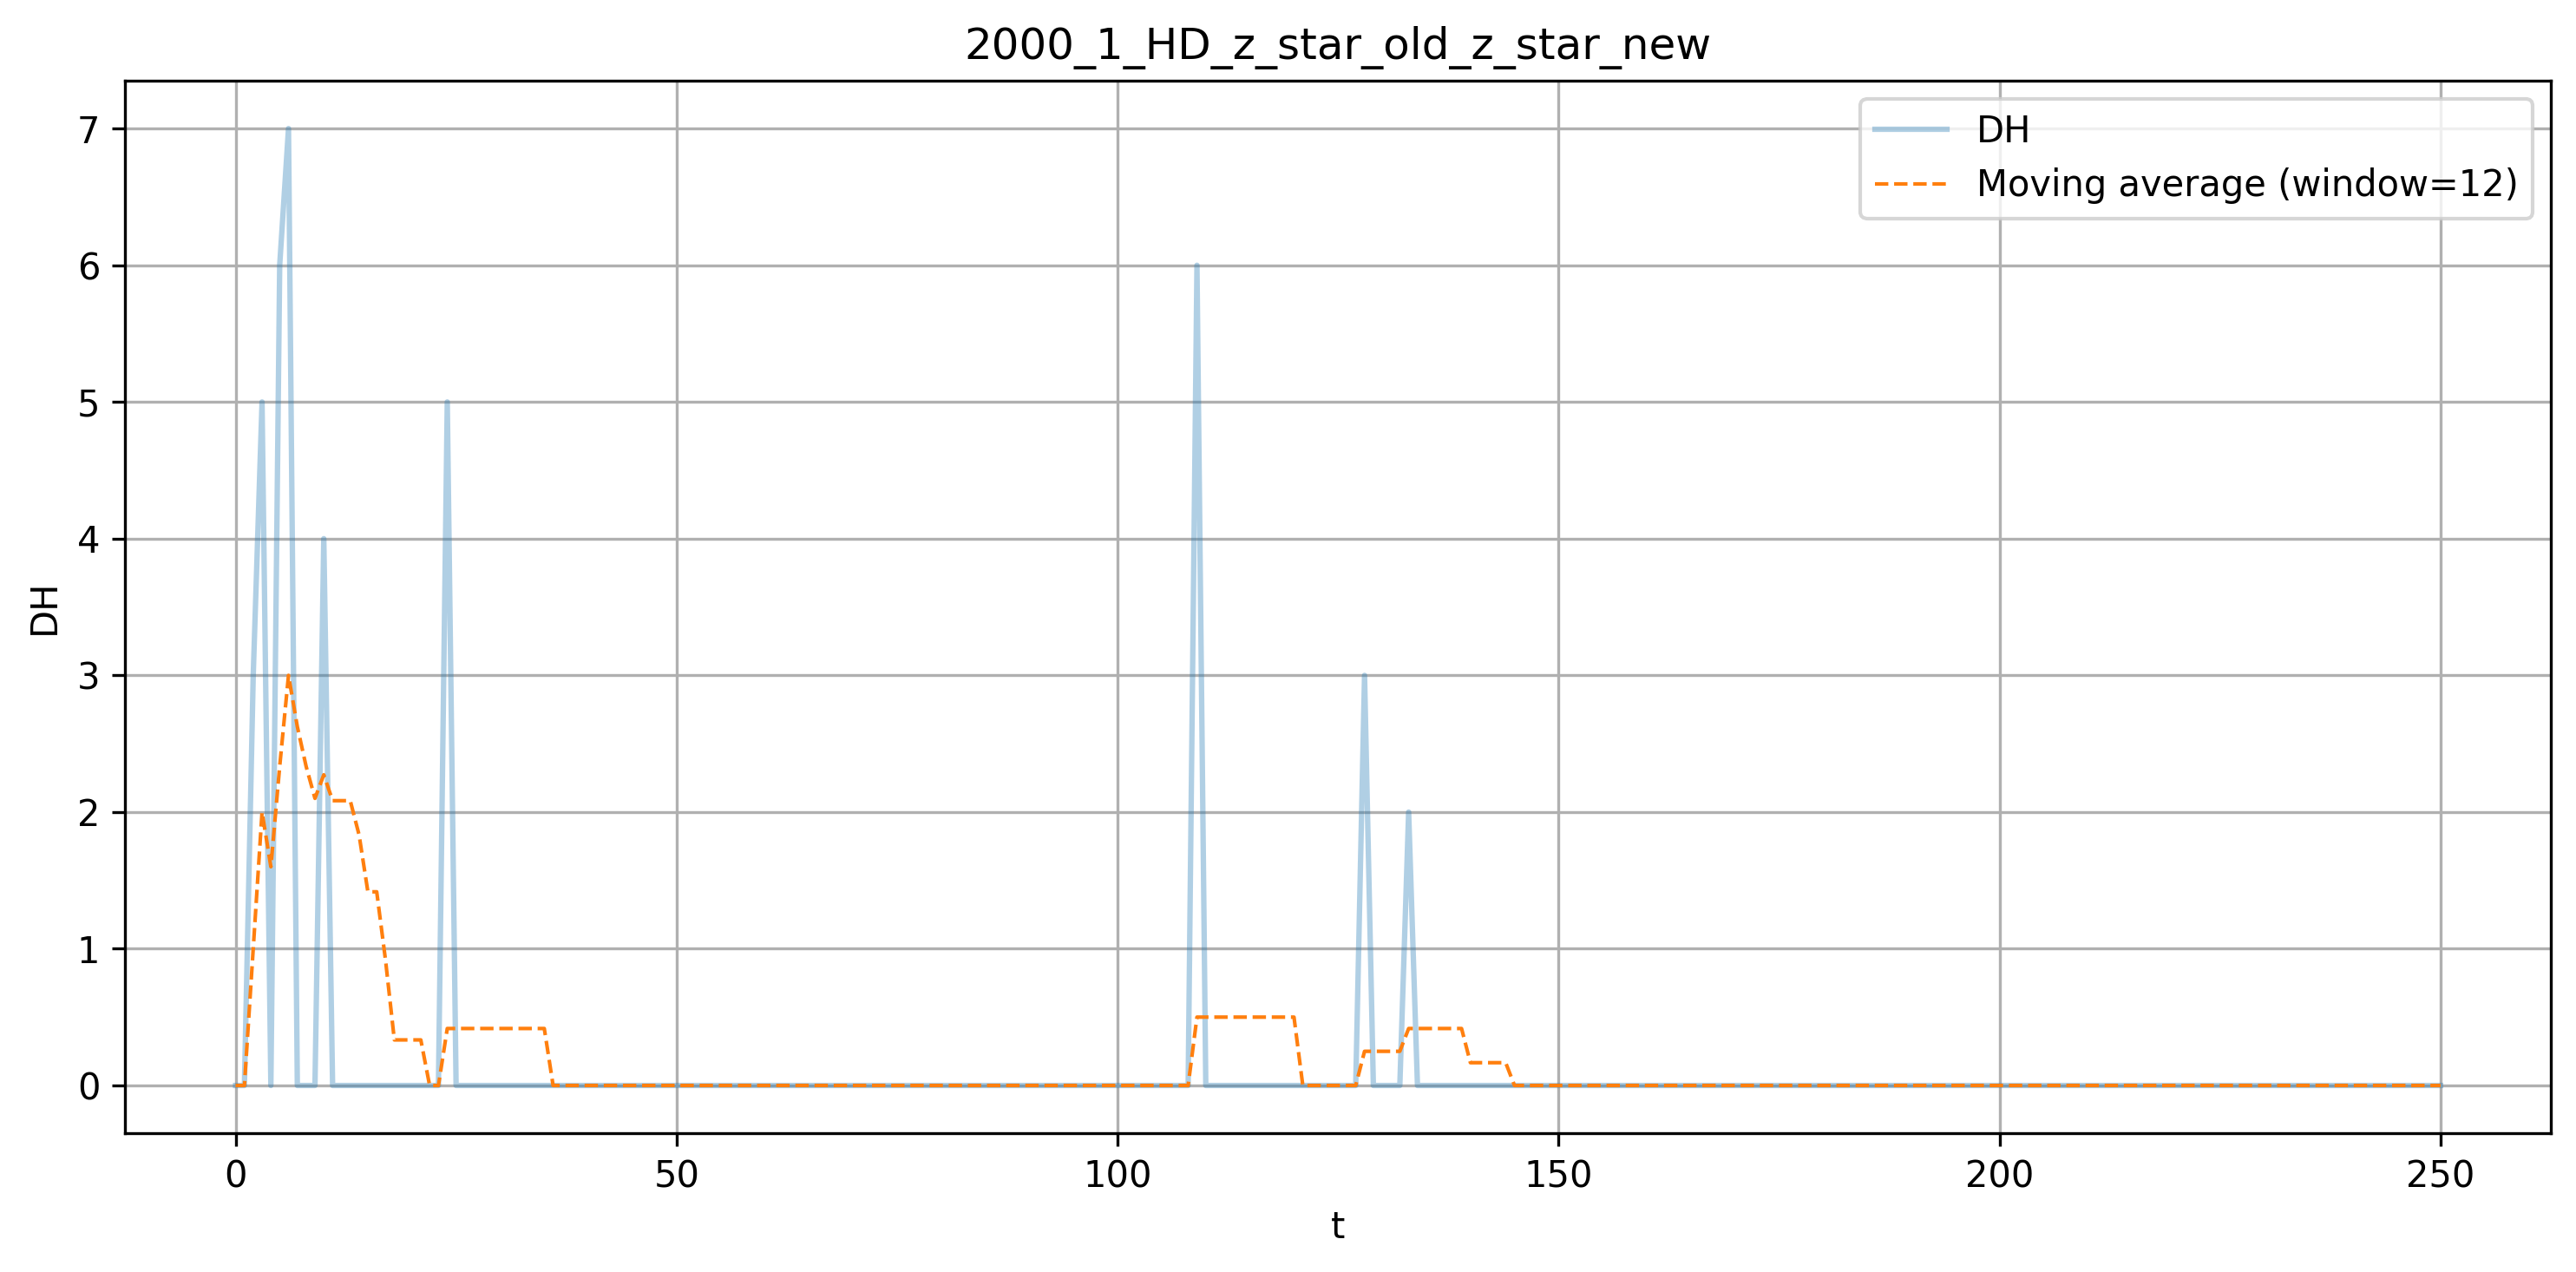
\includegraphics[width=\linewidth]{../Quantum-Annealing-for-solving-QUBO-Problems/test/Lambda_dinamico/ksp_1/lambda_650_dot_C/2000_1_HD_z_star_old_z_star_new.png}
    \caption{\(d_H(z_\star^{old}, z_\star^{new})\) con \(\lambda_1\)}
    \label{fig:hd-zstarold-zstarnew-lambda1}
\end{subfigure}
\hfill
\begin{subfigure}{0.495\textwidth}
    \centering
    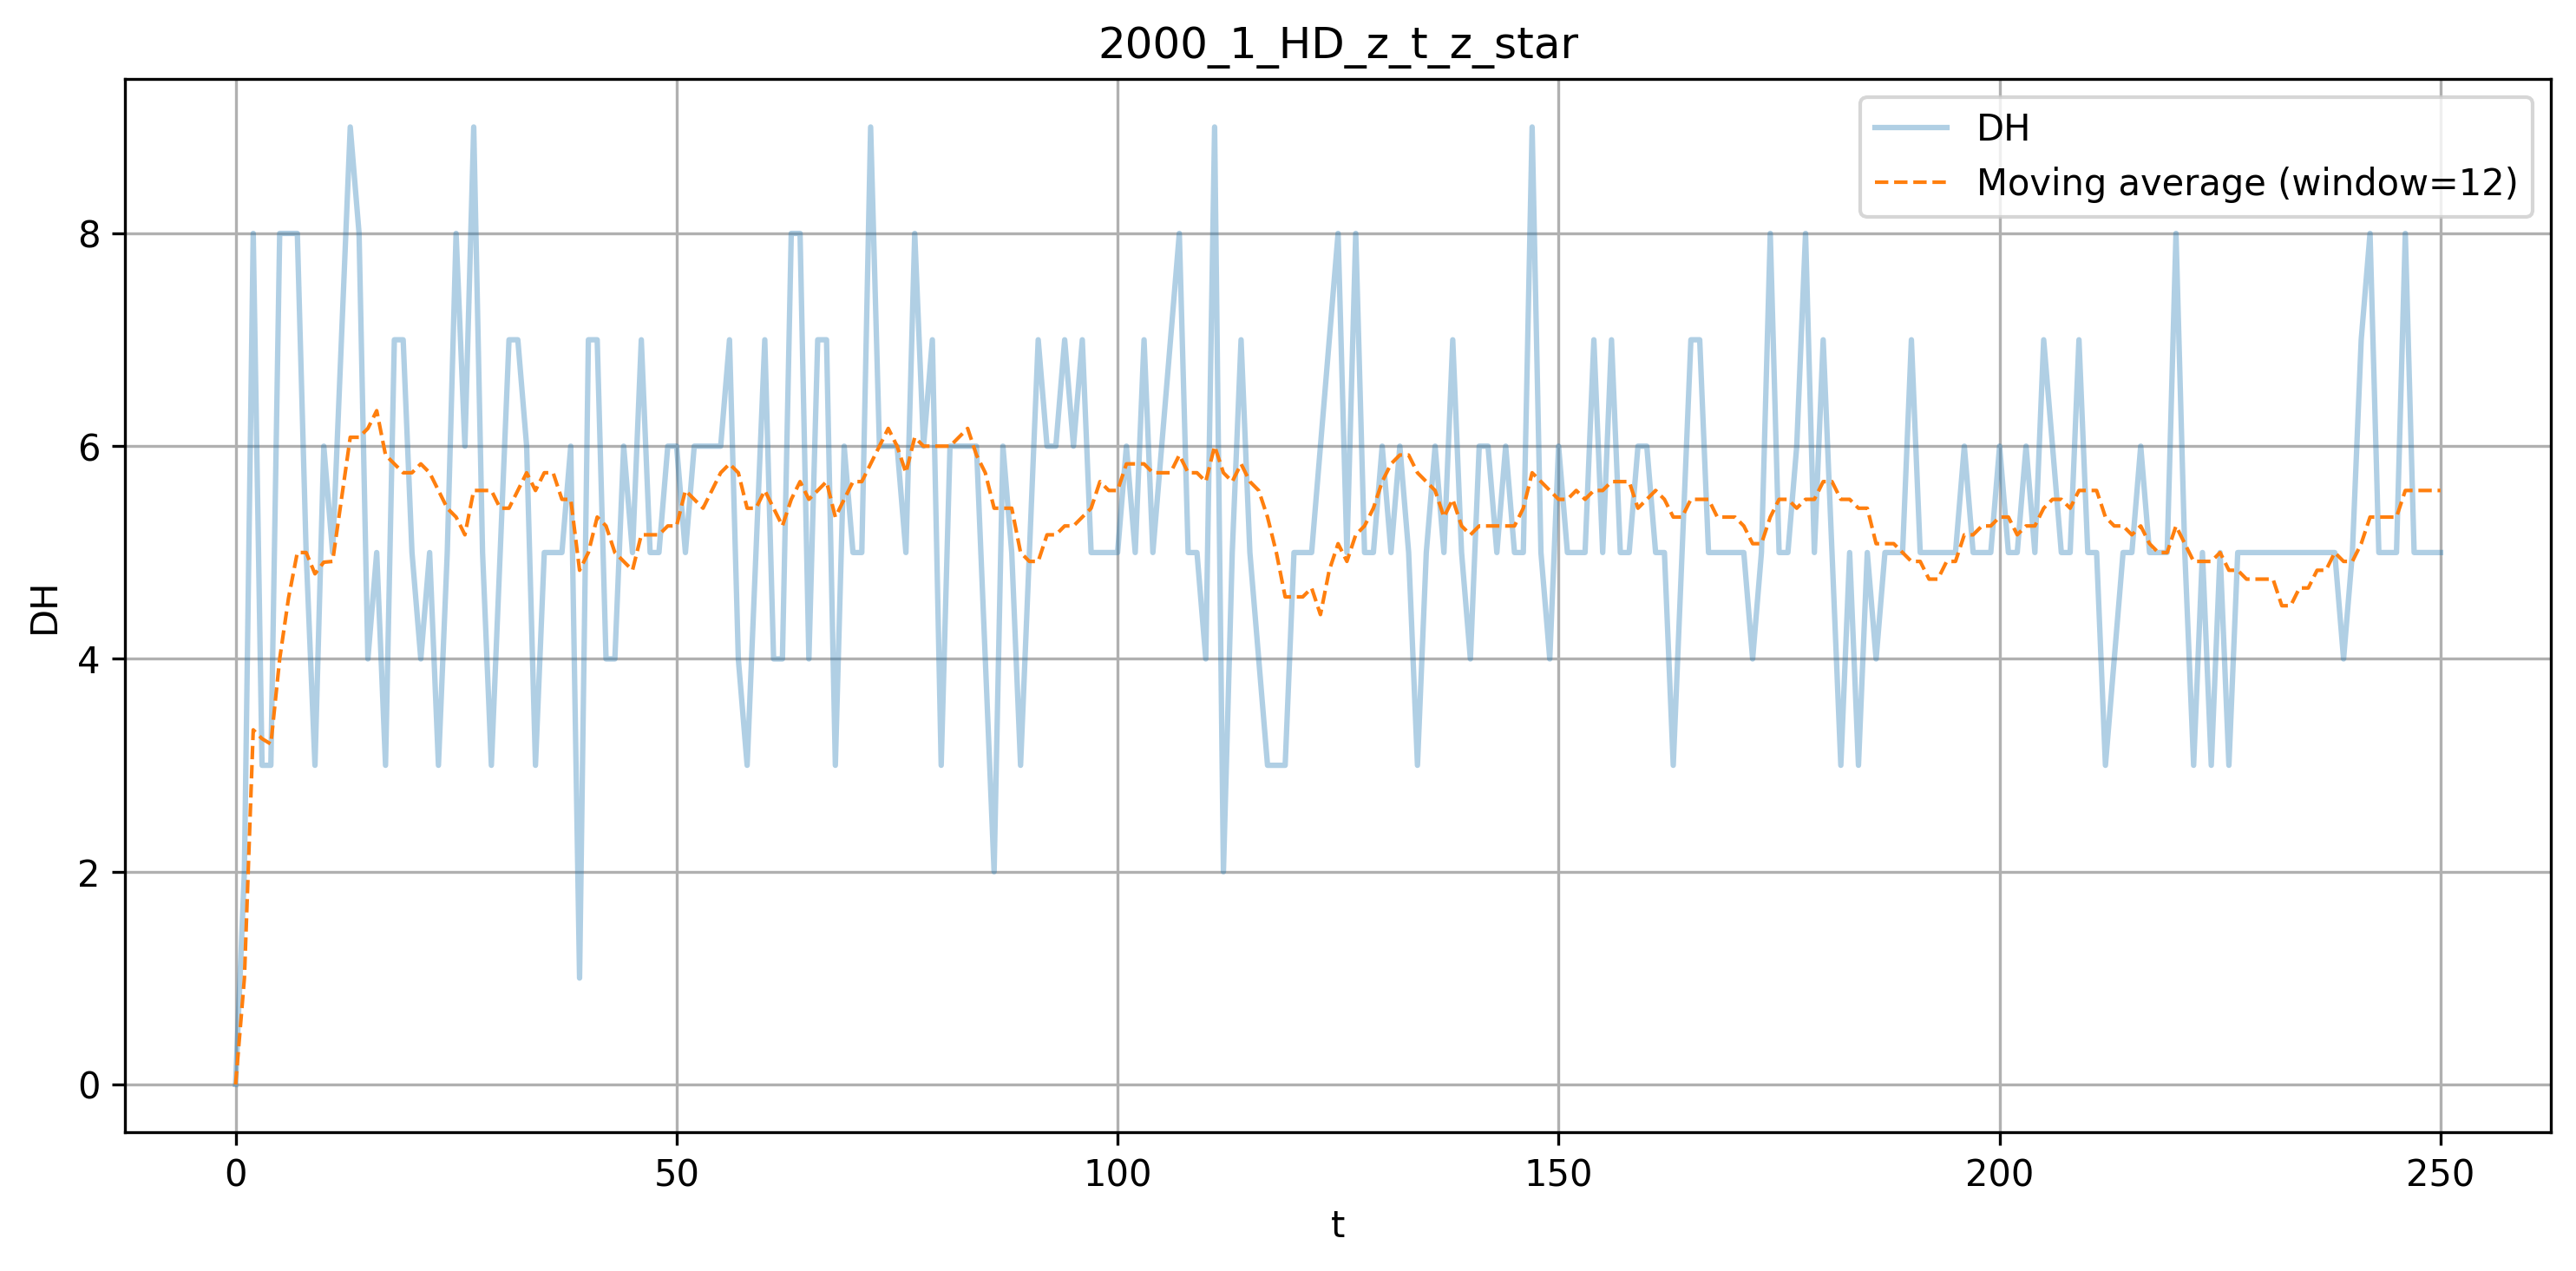
\includegraphics[width=\linewidth]{../Quantum-Annealing-for-solving-QUBO-Problems/test/Lambda_dinamico/ksp_1/lambda_650_dot_C/2000_1_HD_z_t_z_star.png}
    \caption{\(d_H(z_t, z_\star)\) con \(\lambda_1\)}
    \label{fig:hd-zt-zstar-lambda1}
\end{subfigure}

\vspace{0.35cm}

\begin{subfigure}{0.495\textwidth}
    \centering
    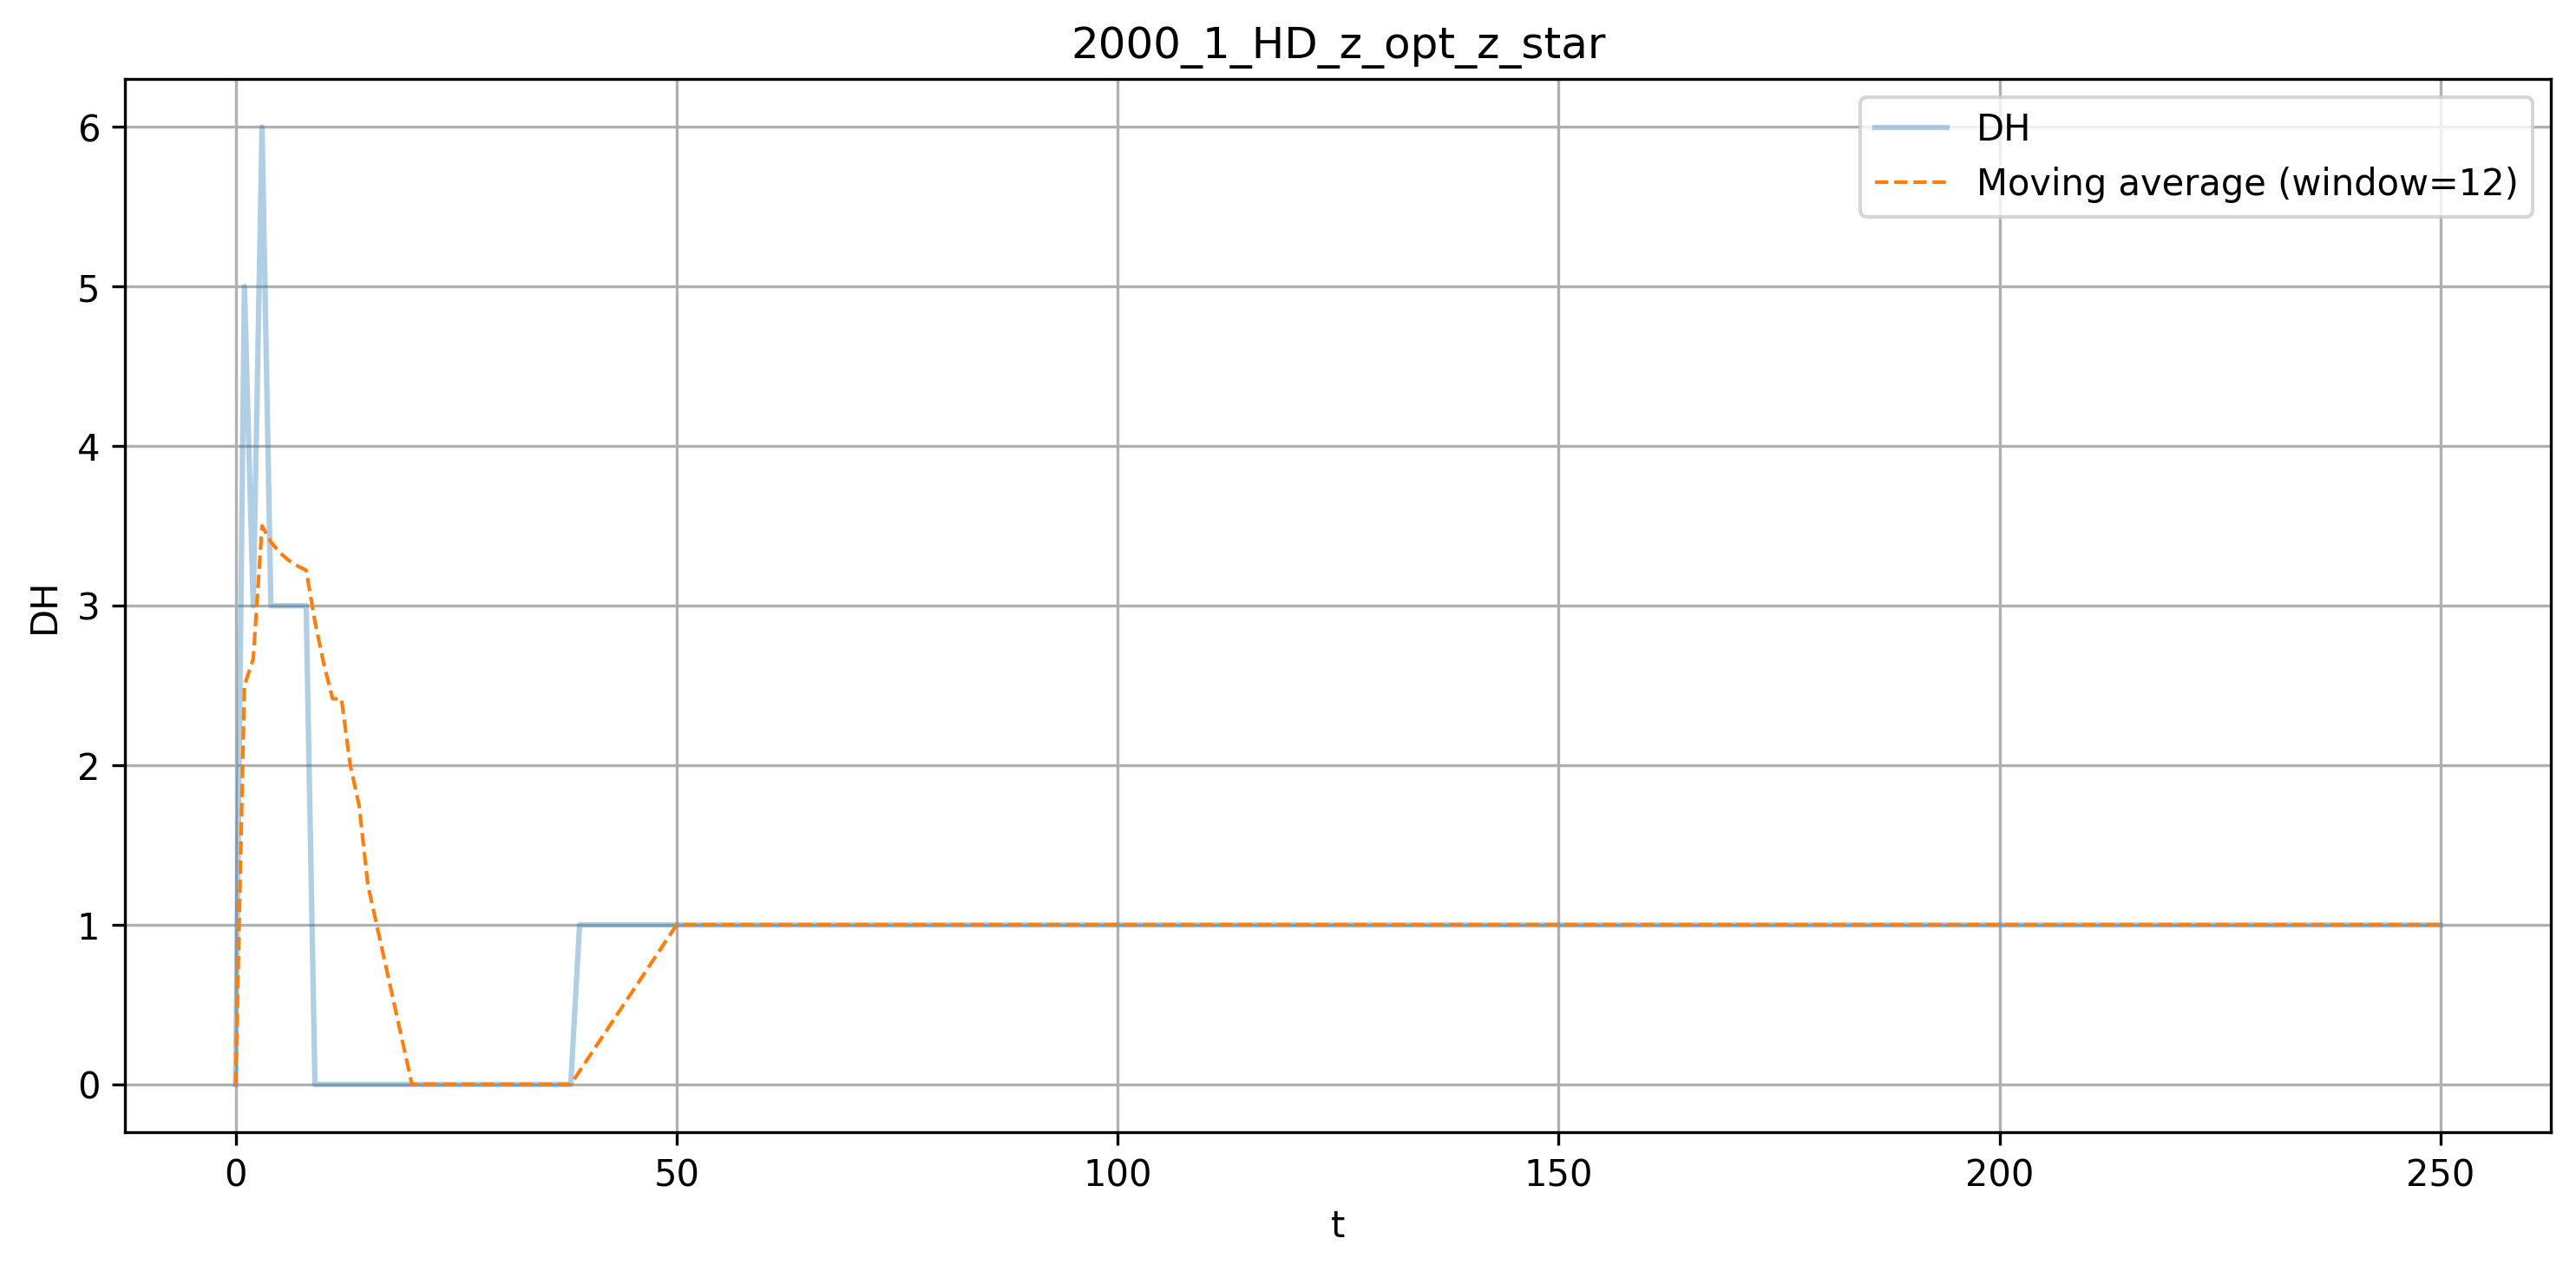
\includegraphics[width=\linewidth]{../Quantum-Annealing-for-solving-QUBO-Problems/test/Lambda_dinamico/ksp_1/lambda_650_dot_C/2000_1_HD_z_opt_z_star.png}
    \caption{\(d_H(z_{opt}, z_\star)\) con \(\lambda_1\)}
    \label{fig:hd-zopt-zstar-lambda1}
\end{subfigure}
\hfill
\begin{subfigure}{0.495\textwidth}
    \centering
    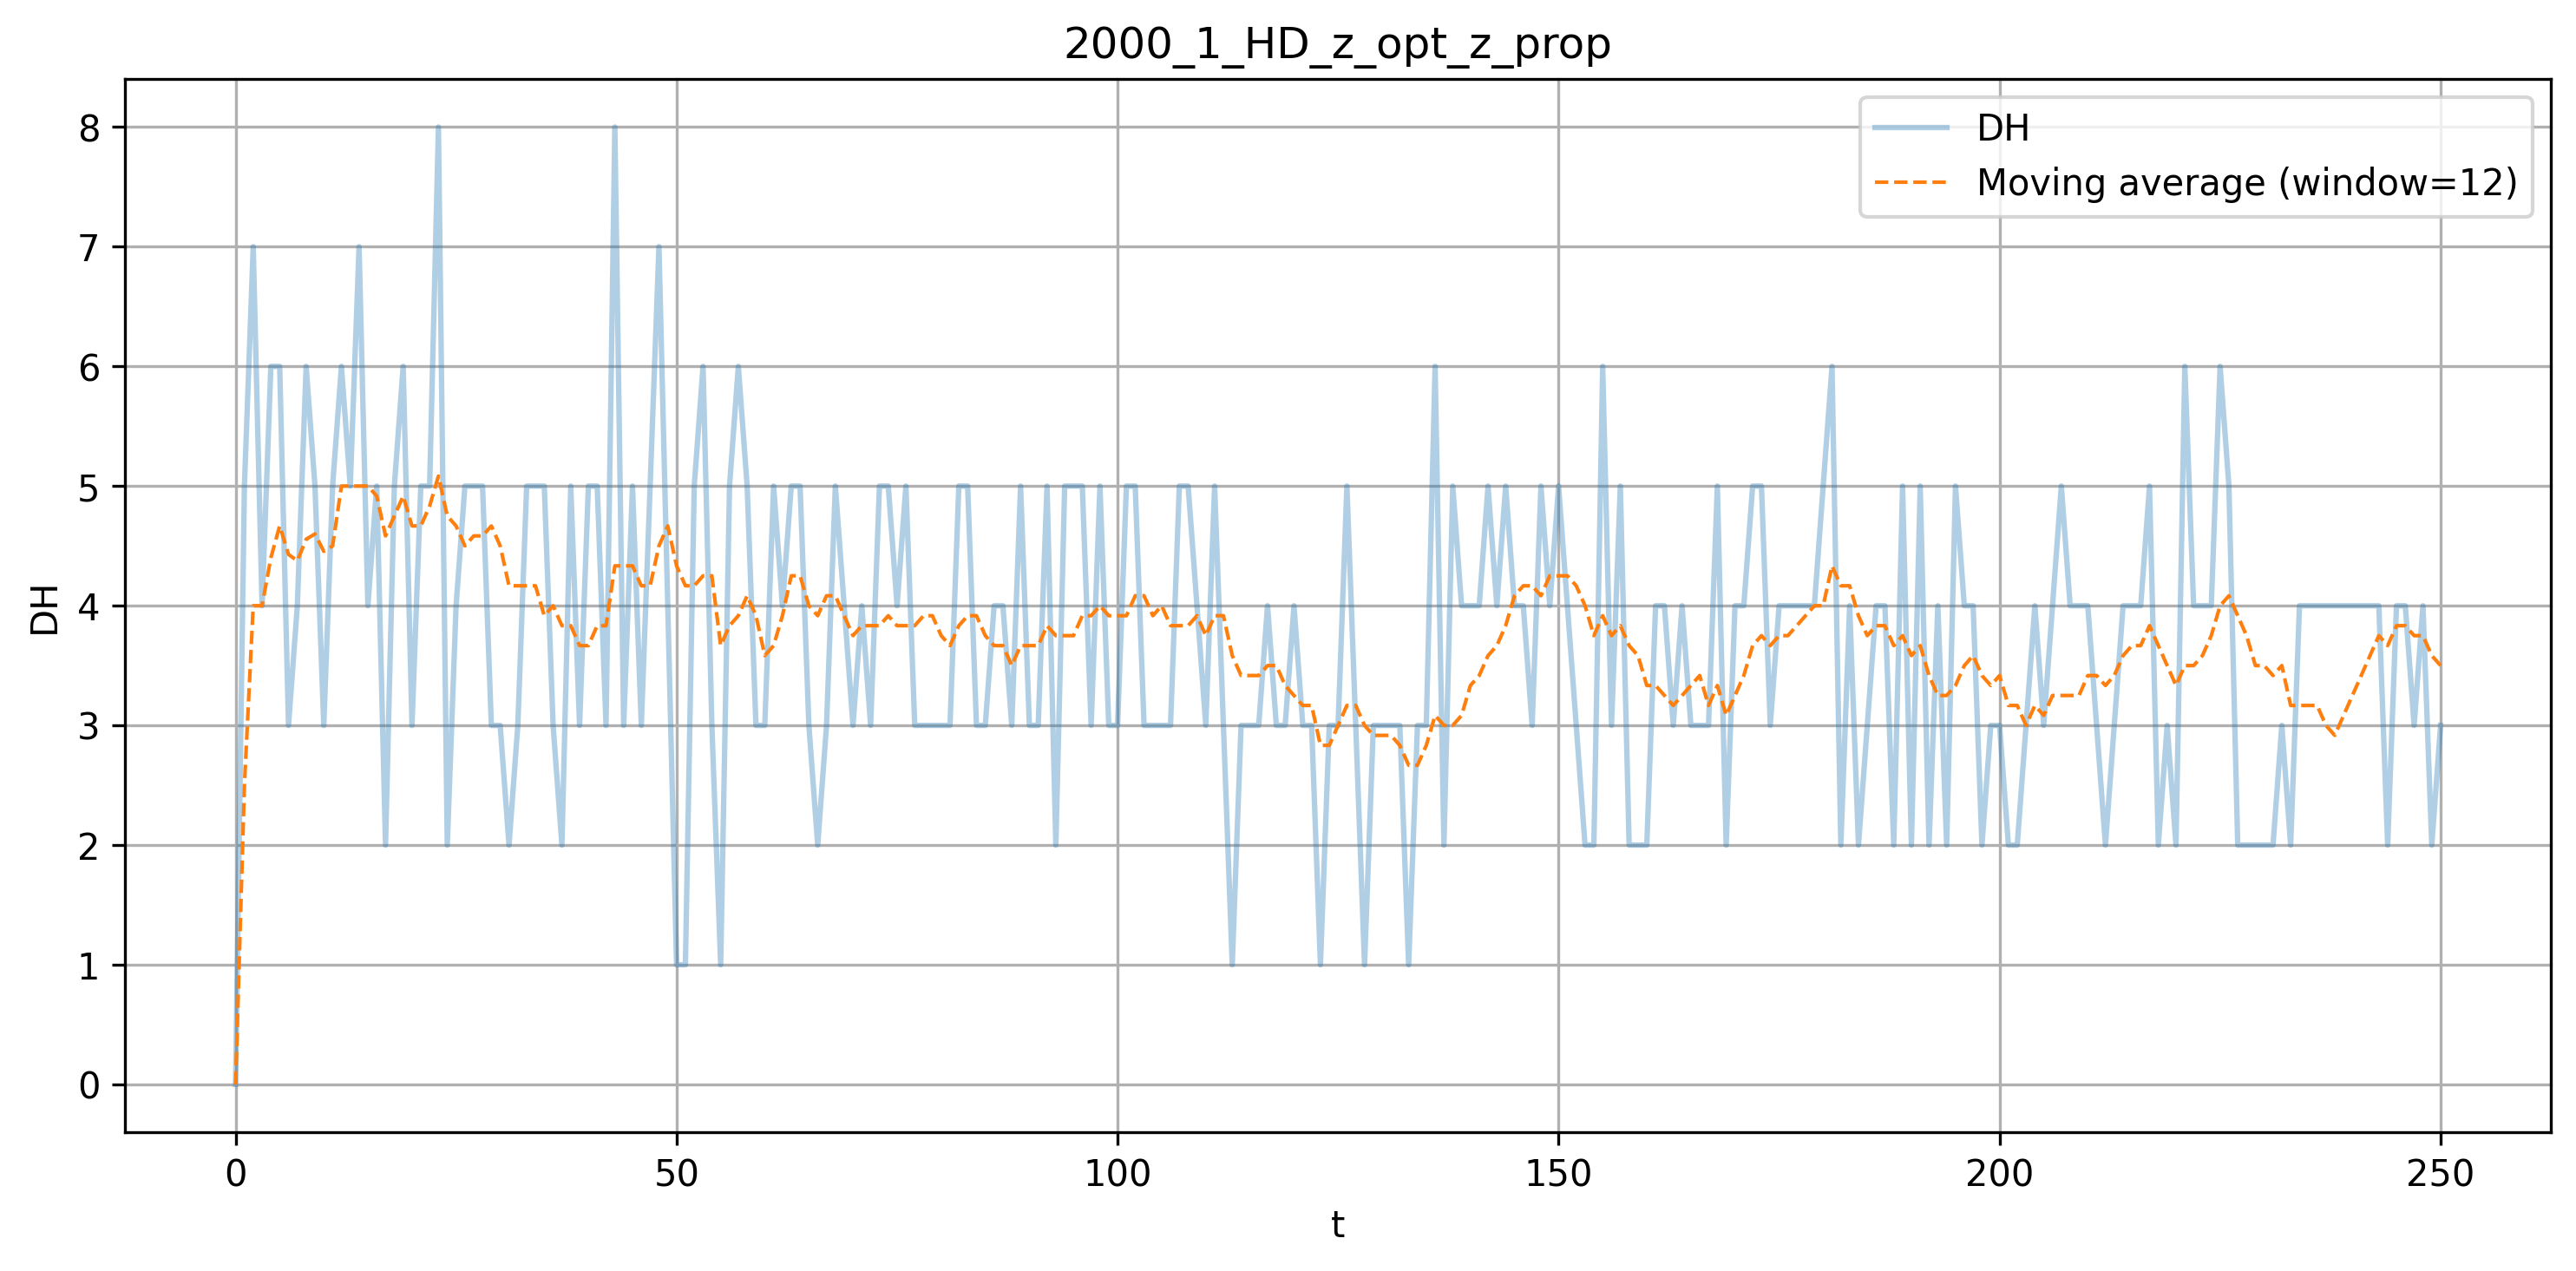
\includegraphics[width=\linewidth]{../Quantum-Annealing-for-solving-QUBO-Problems/test/Lambda_dinamico/ksp_1/lambda_650_dot_C/2000_1_HD_z_opt_z_prop.png}
    \caption{\(d_H(z_{opt}, z_t)\) con \(\lambda_1\)}
    \label{fig:hd-zopt-zprop-lambda1}
\end{subfigure}

\vspace{0.35cm}

\begin{subfigure}{0.495\textwidth}
    \centering
    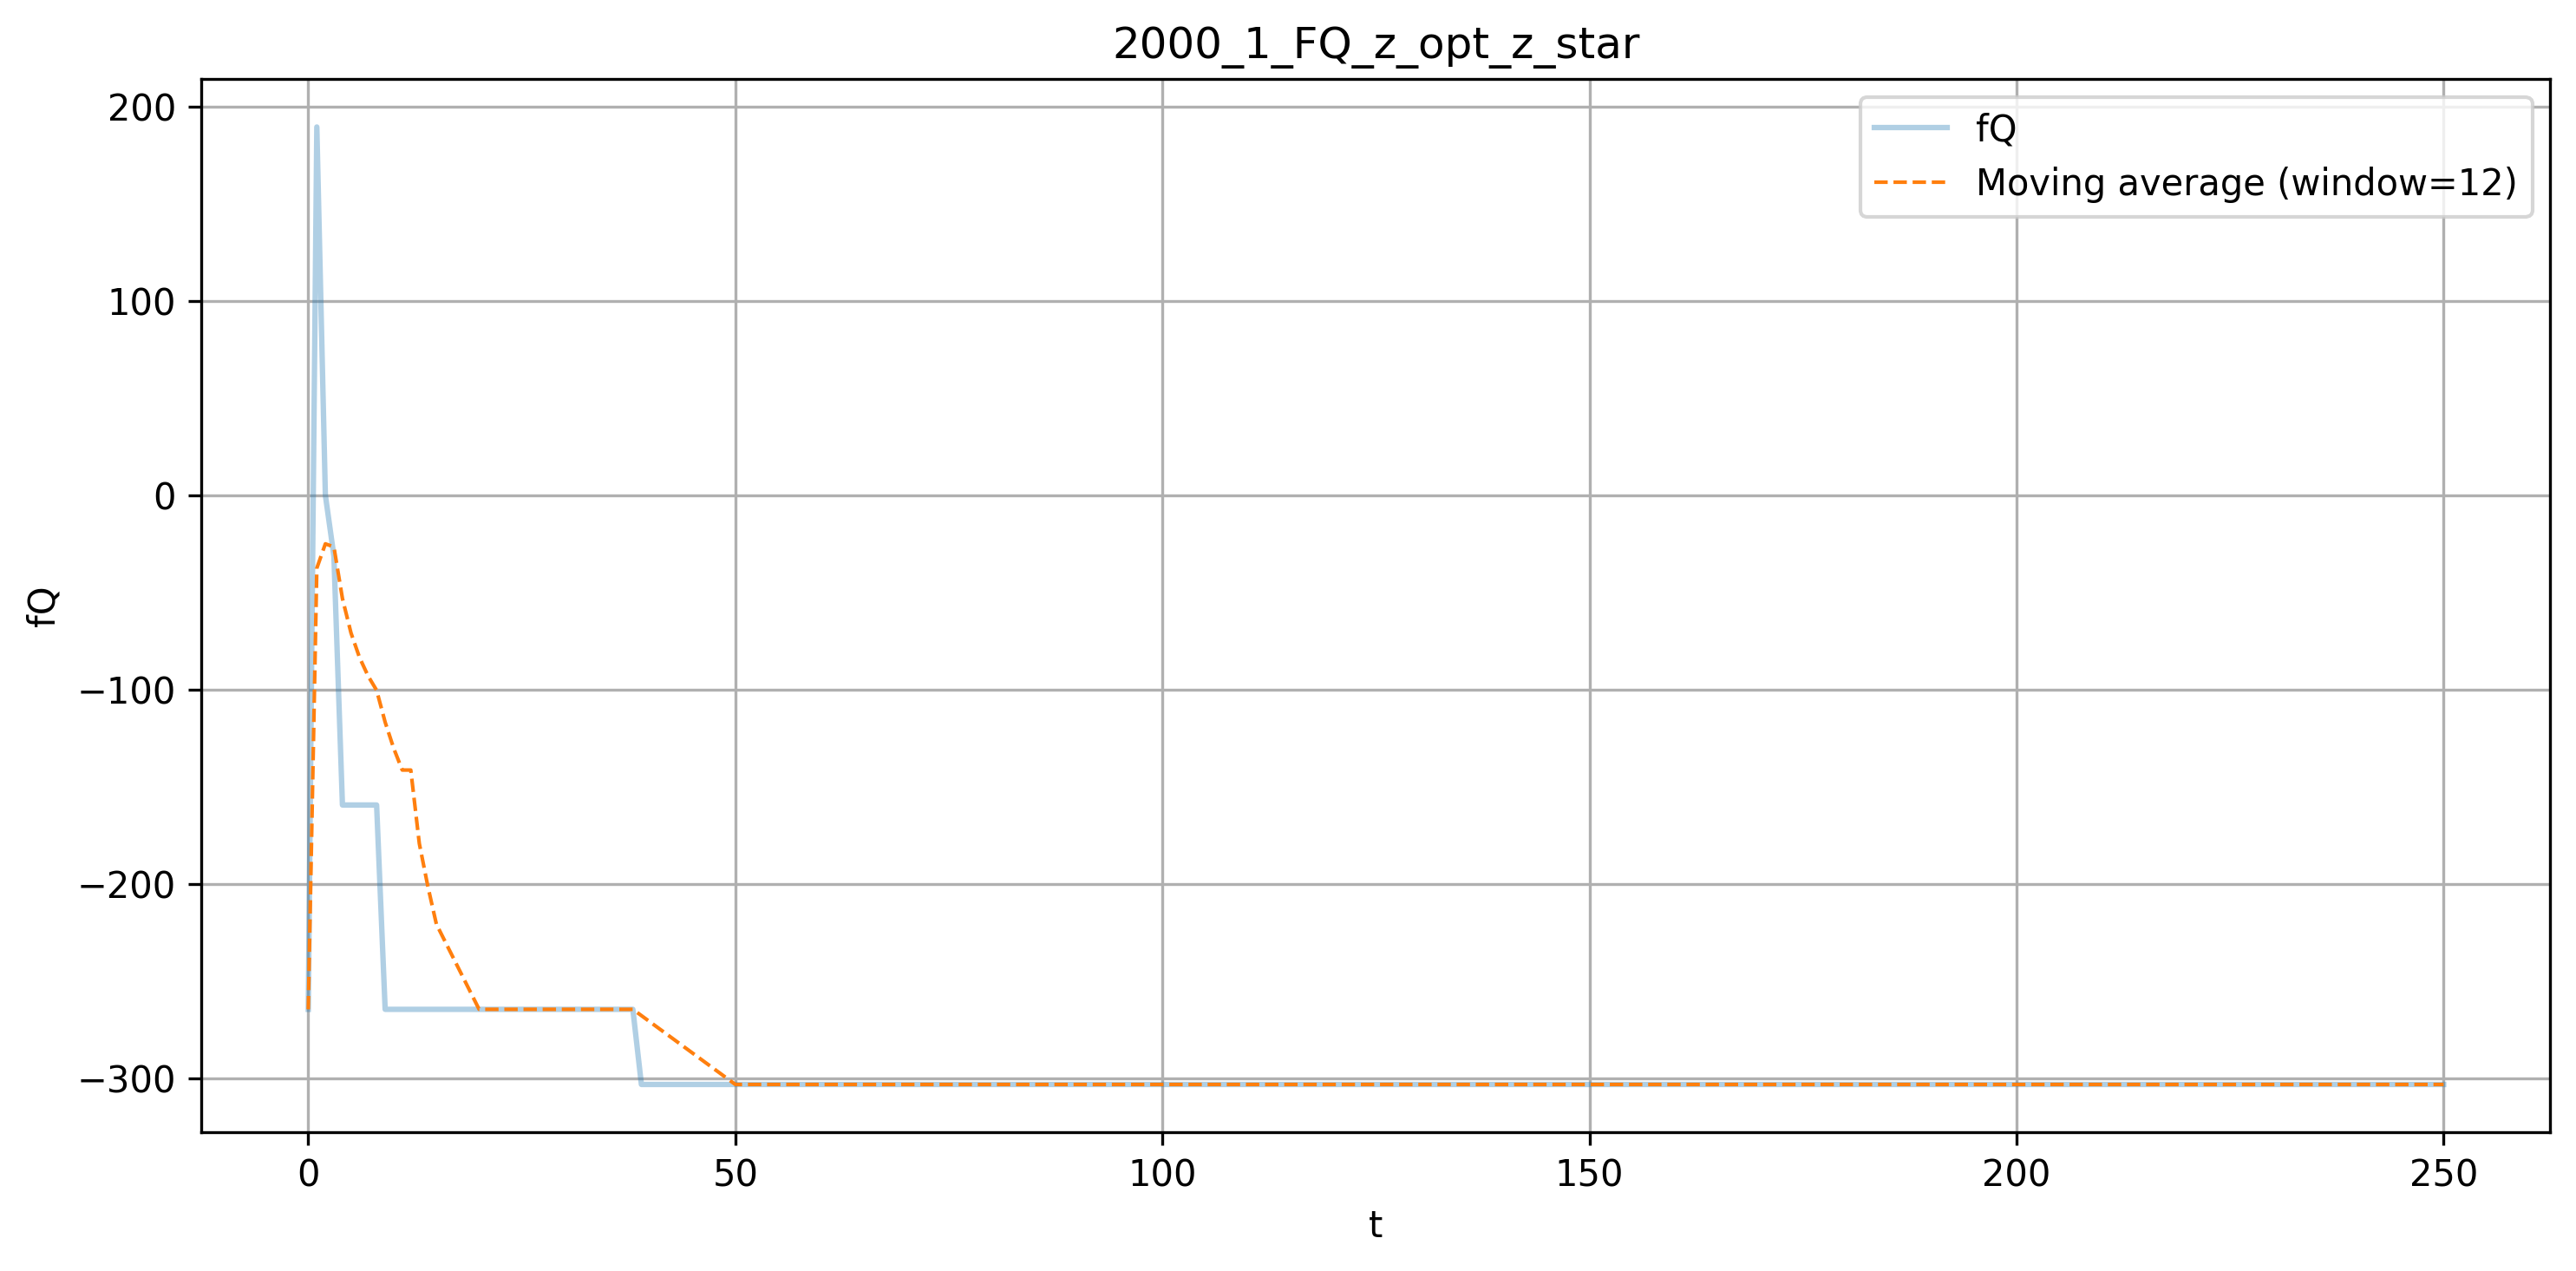
\includegraphics[width=\linewidth]{../Quantum-Annealing-for-solving-QUBO-Problems/test/Lambda_dinamico/ksp_1/lambda_650_dot_C/2000_1_FQ_z_opt_z_star.png}
    \caption{\(f_Q(z_\star)\) con \(\lambda_1\)}
    \label{fig:fQ-zstar-lambda1}
\end{subfigure}
\hfill
\begin{subfigure}{0.495\textwidth}
    \centering
    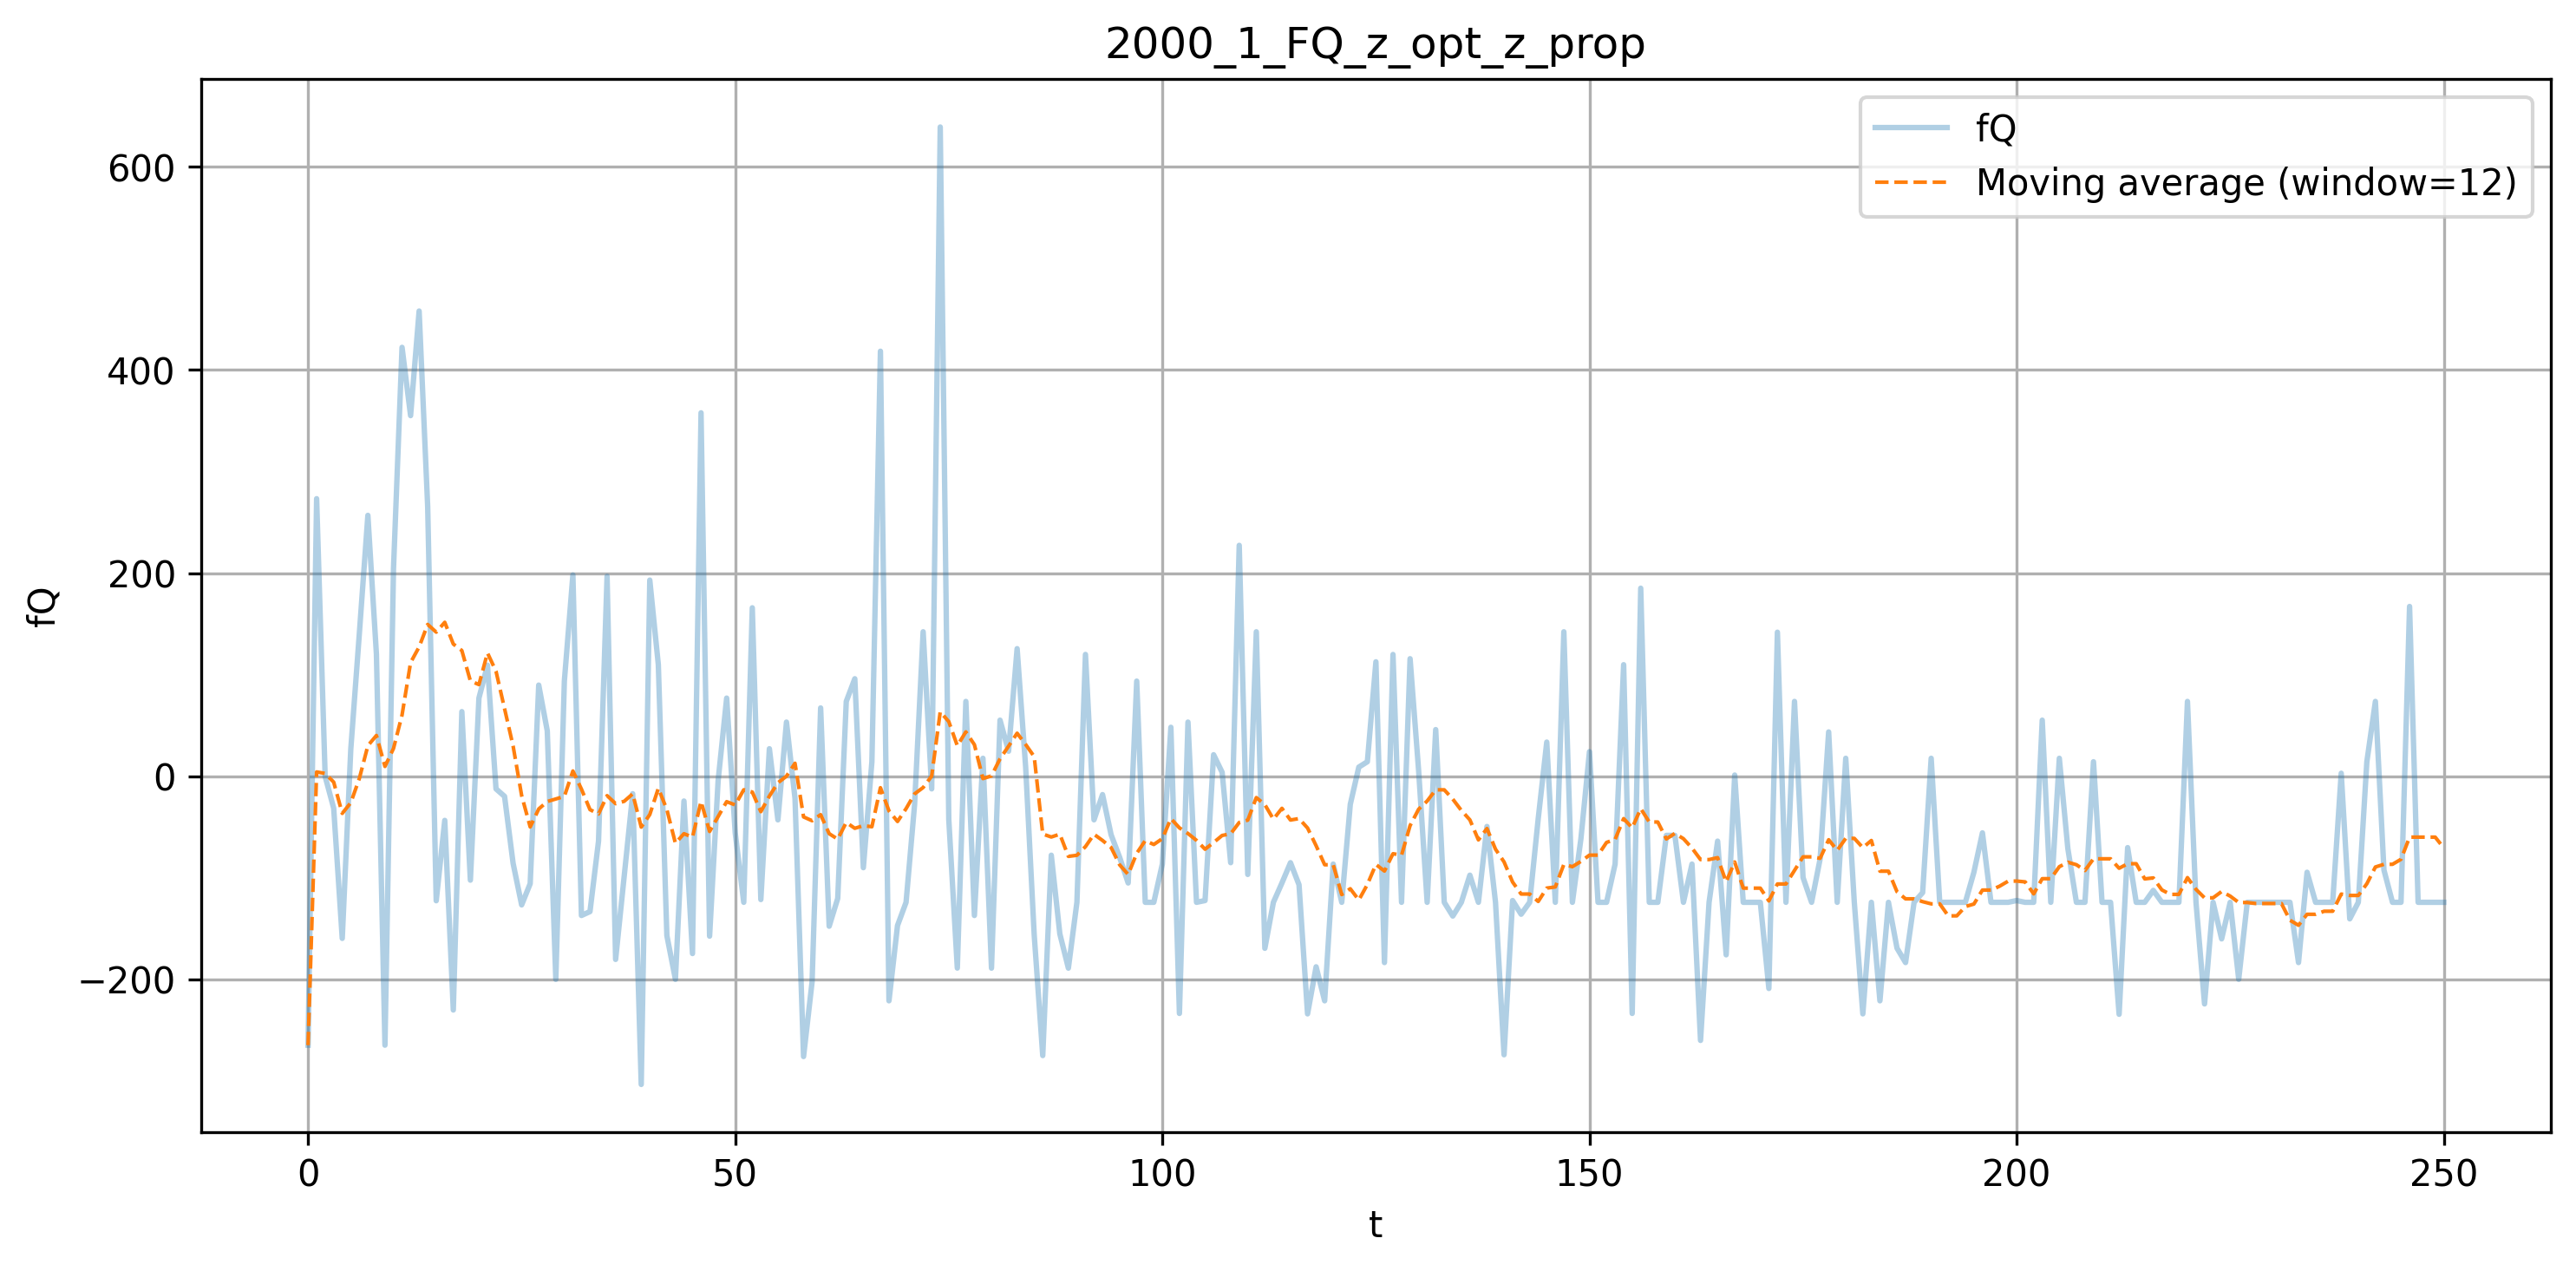
\includegraphics[width=\linewidth]{../Quantum-Annealing-for-solving-QUBO-Problems/test/Lambda_dinamico/ksp_1/lambda_650_dot_C/2000_1_FQ_z_opt_z_prop.png}
    \caption{\(f_Q(z_t)\) con \(\lambda_1\)}
    \label{fig:fQ-zt-lambda1}
\end{subfigure}
\label{fig:confronto-hamming-ksp11}
\end{figure}

\begin{figure}[H]
\centering
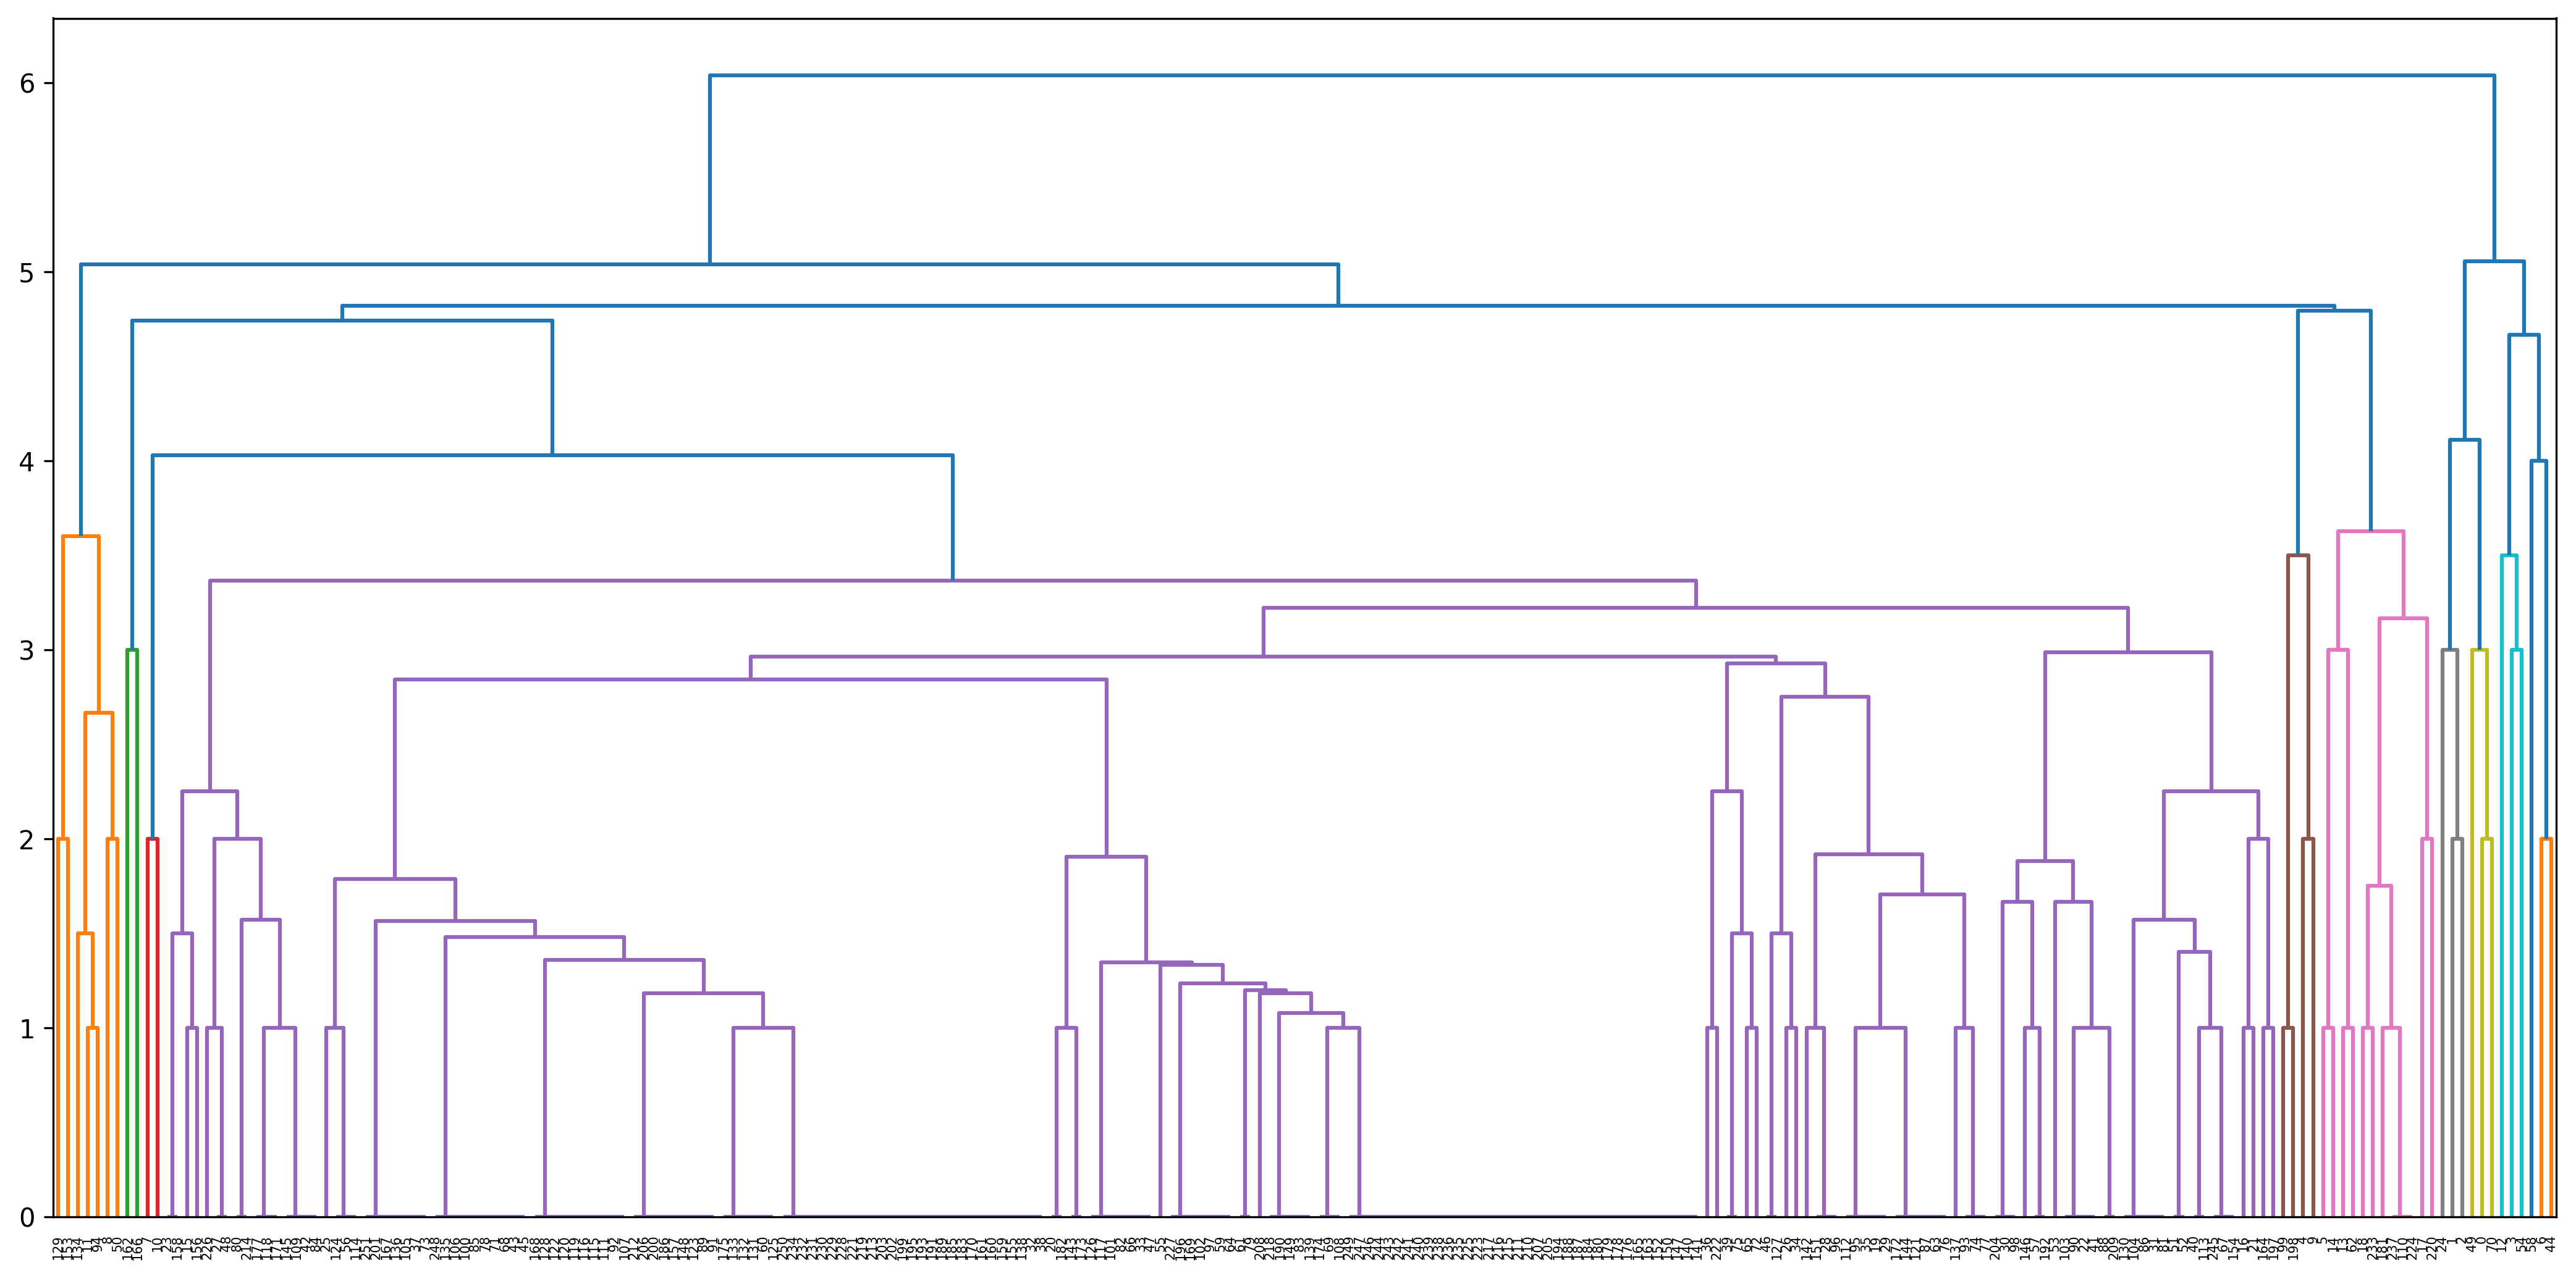
\includegraphics[width=\linewidth]{../Quantum-Annealing-for-solving-QUBO-Problems/test/Lambda_dinamico/ksp_1/lambda_650_dot_C/dendrogram_2000_1.png}
\caption{Agglomerative Clustering Dendogram}
\label{fig:AgglomerativeClustering-ksp1}
\end{figure}
\clearpage

\begin{figure}[H]
\centering
\begin{subfigure}{0.495\textwidth}
    \centering
    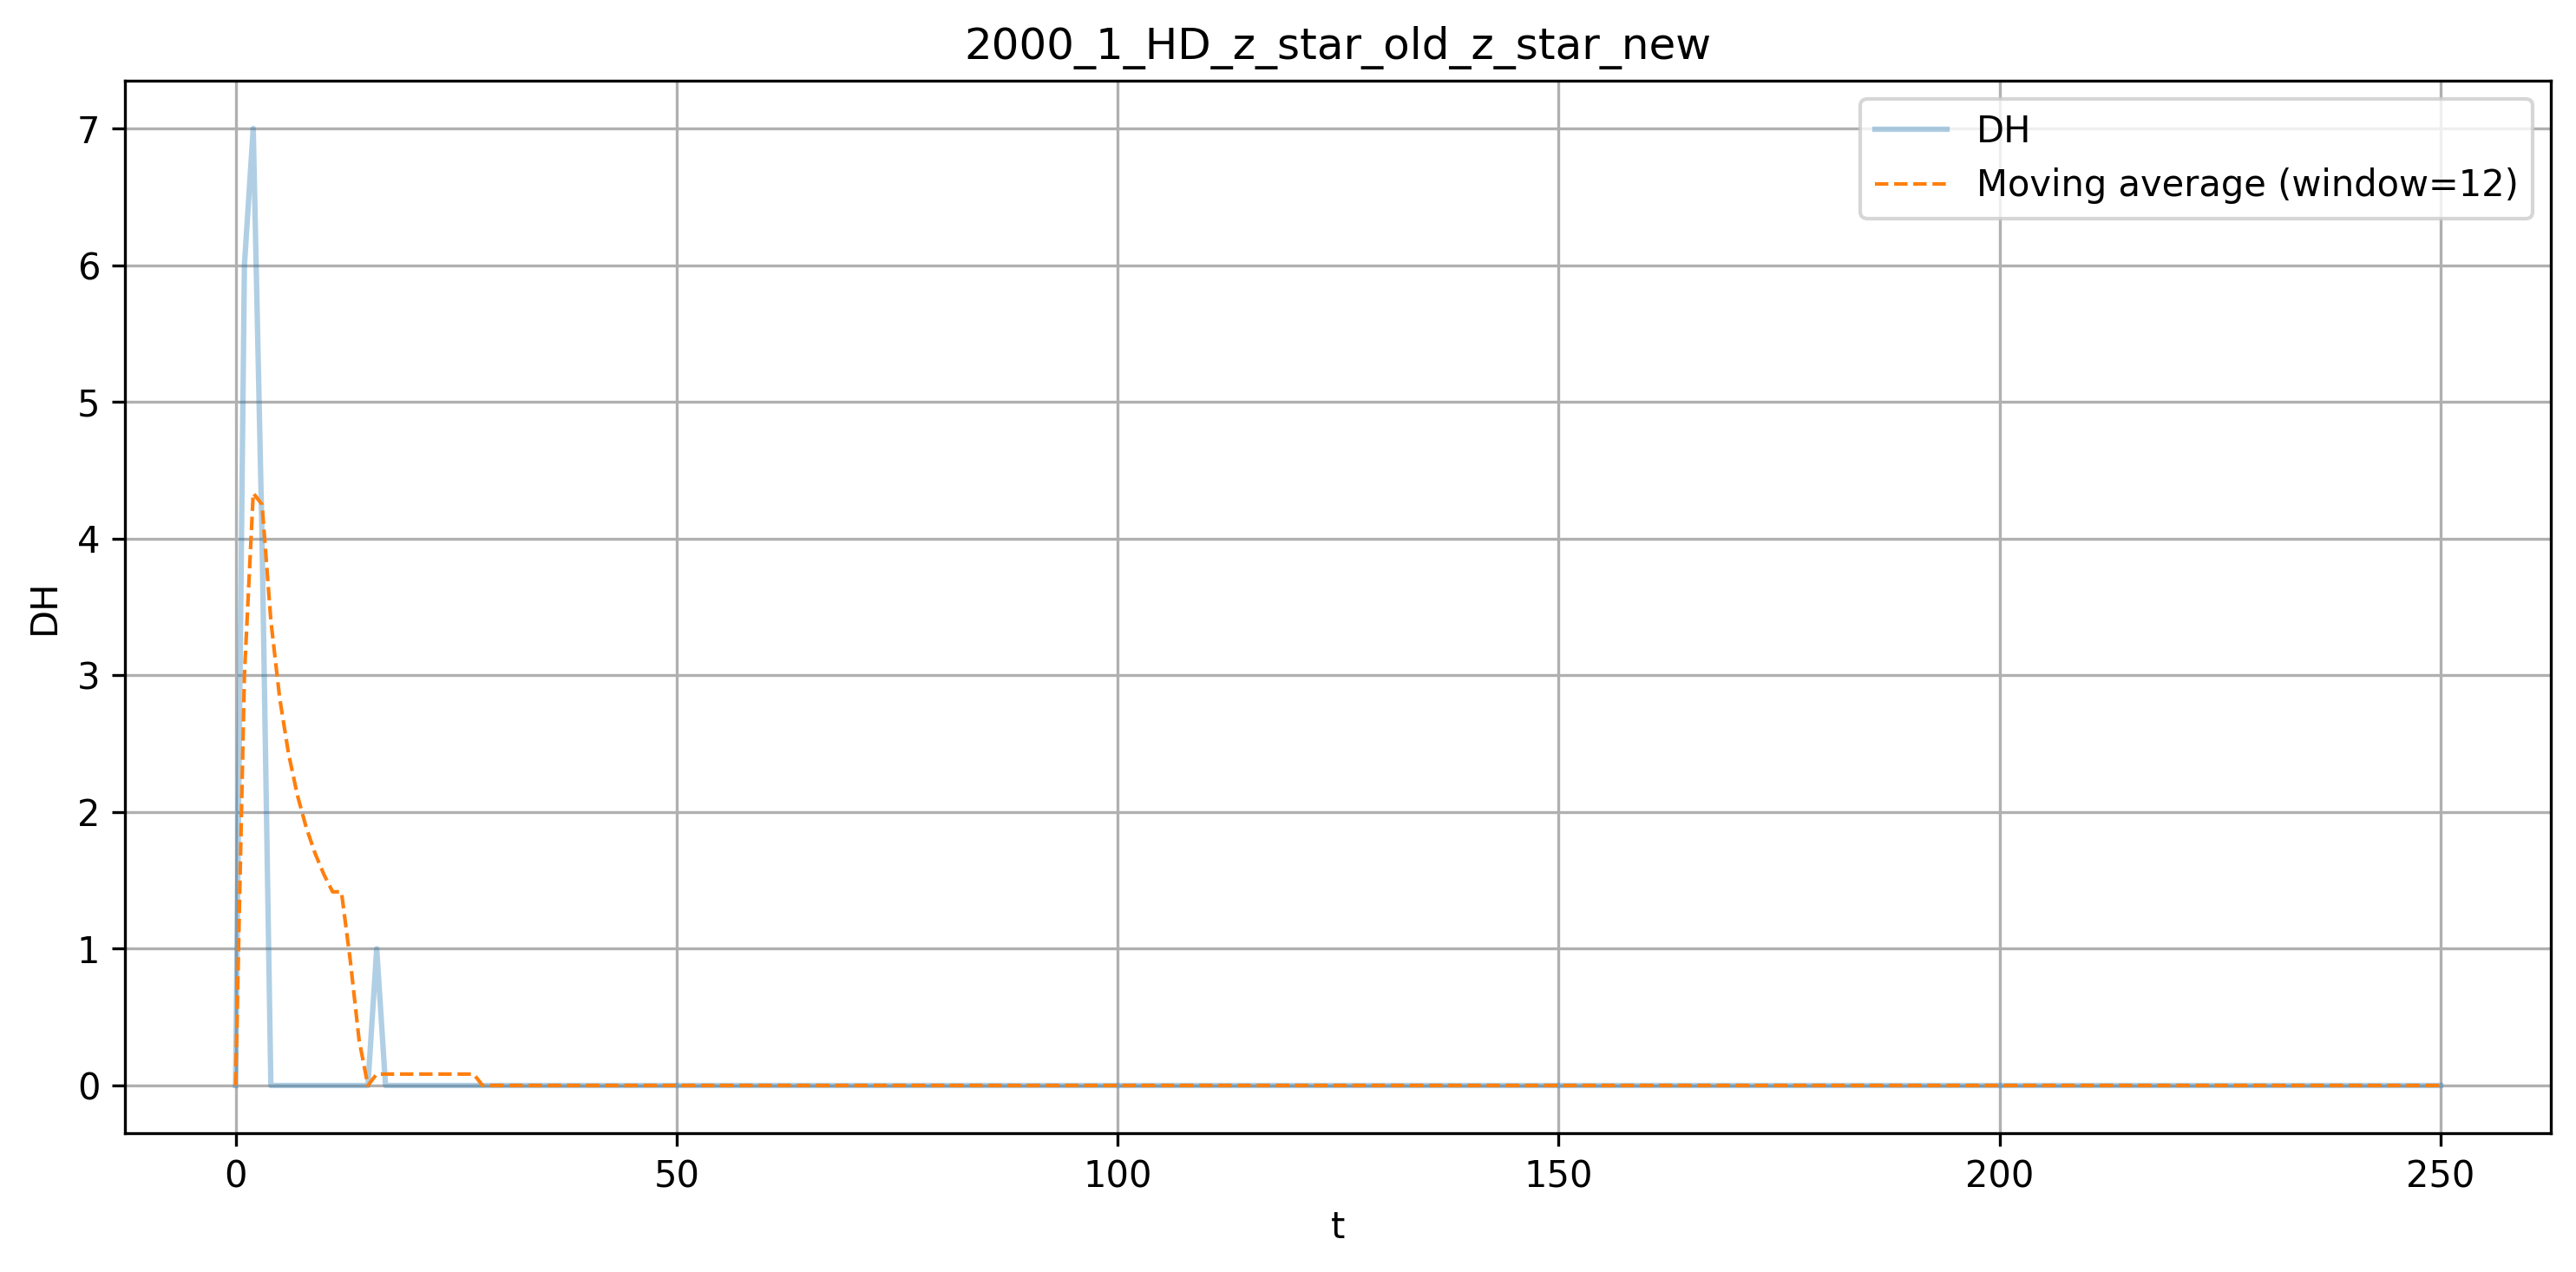
\includegraphics[width=\linewidth]{../Quantum-Annealing-for-solving-QUBO-Problems/test/Lambda_dinamico/ksp_1/lambda_div_3/2000_1_HD_z_star_old_z_star_new.png}
    \caption{\(d_H(z_\star^{old}, z_\star^{new})\) con \(\lambda_2\)}
    \label{fig:hd-zstarold-zstarnew-lambda2}
\end{subfigure}
\hfill
\begin{subfigure}{0.495\textwidth}
    \centering
    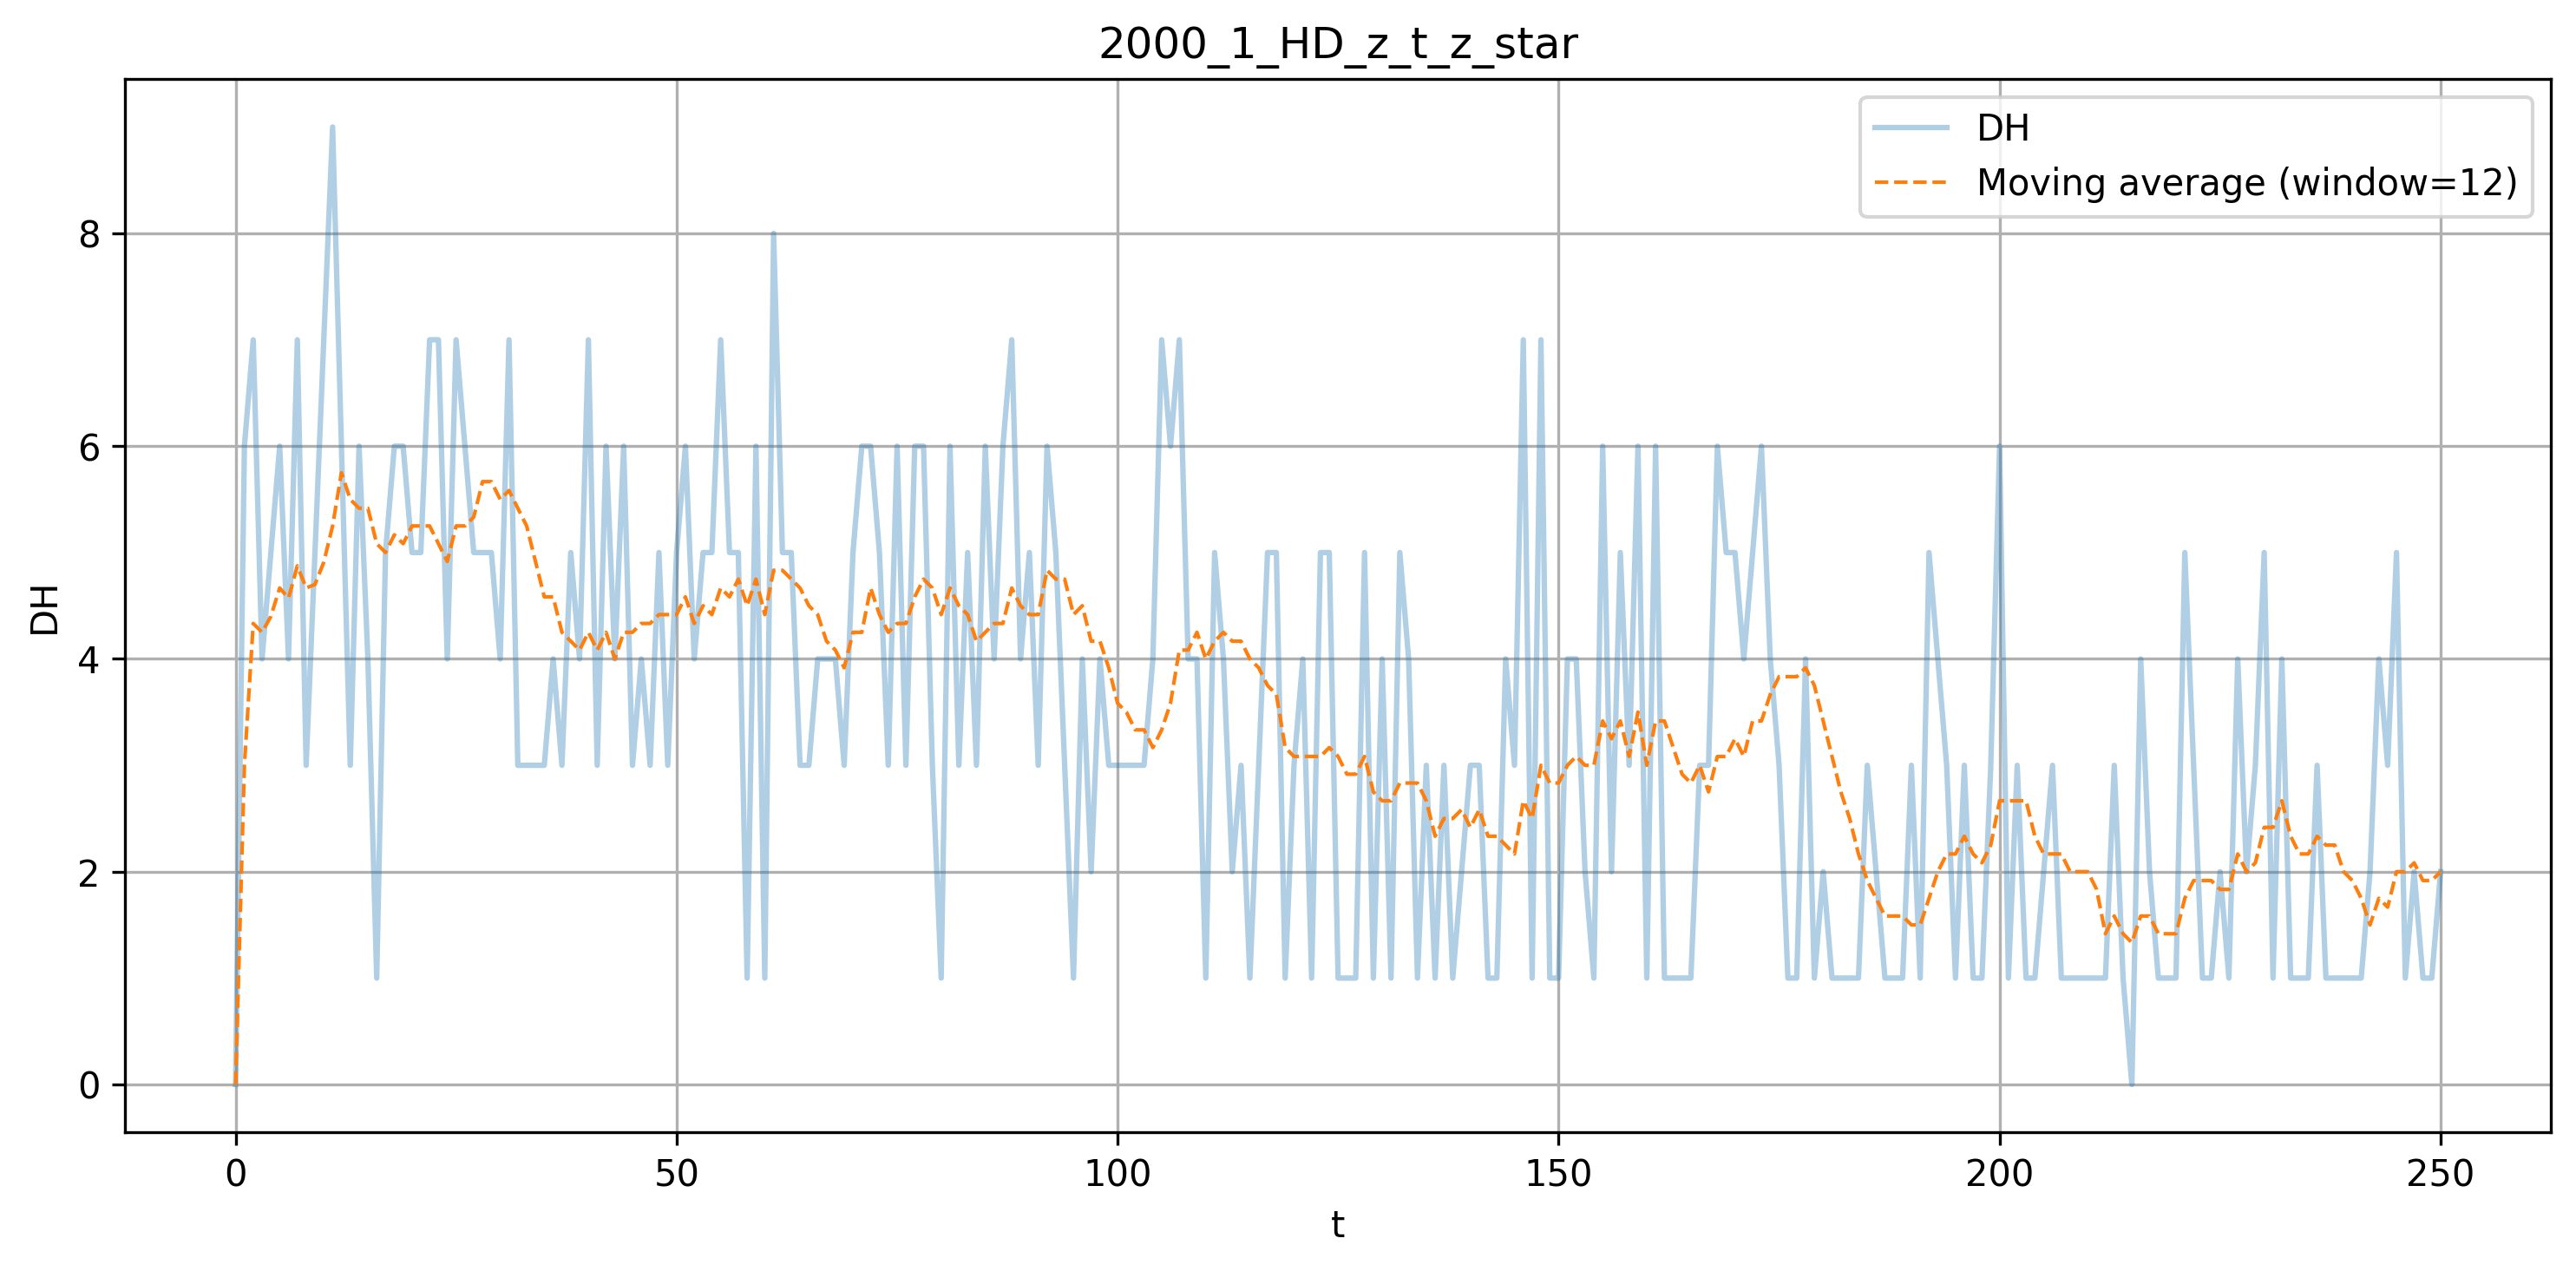
\includegraphics[width=\linewidth]{../Quantum-Annealing-for-solving-QUBO-Problems/test/Lambda_dinamico/ksp_1/lambda_div_3/2000_1_HD_z_t_z_star.png}
    \caption{\(d_H(z_t, z_\star)\) con \(\lambda_2\)}
    \label{fig:hd-zt-zstar-lambda2}
\end{subfigure}

\vspace{0.35cm}

\begin{subfigure}{0.495\textwidth}
    \centering
    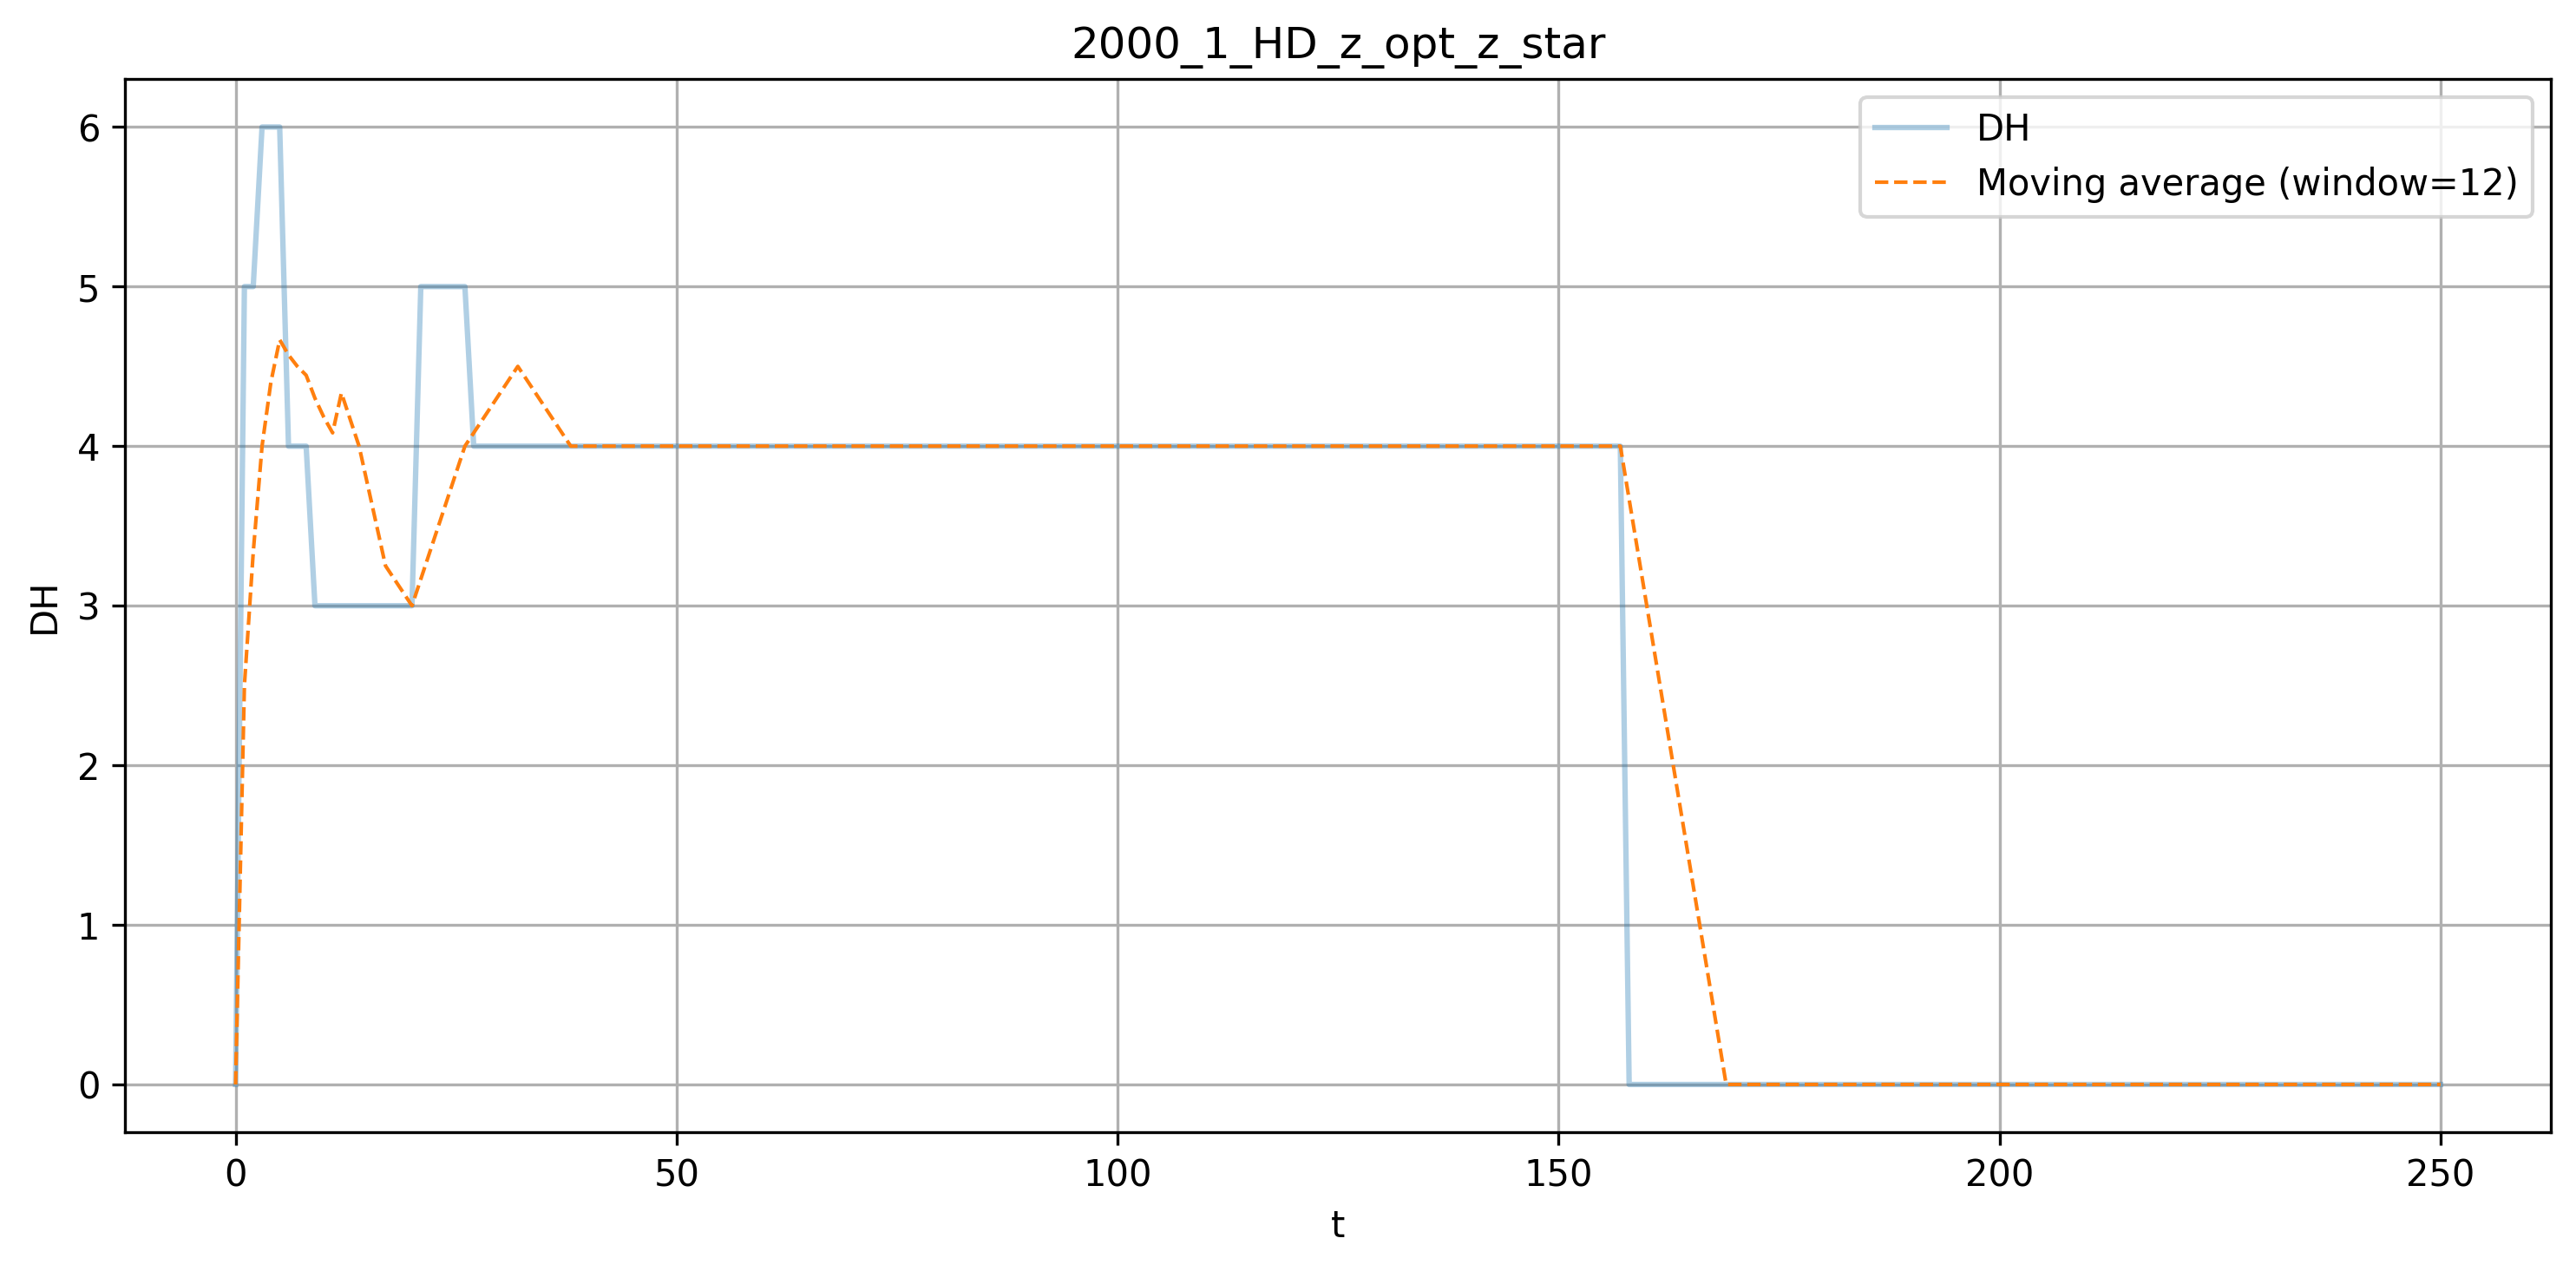
\includegraphics[width=\linewidth]{../Quantum-Annealing-for-solving-QUBO-Problems/test/Lambda_dinamico/ksp_1/lambda_div_3/2000_1_HD_z_opt_z_star.png}
    \caption{\(d_H(z_{opt}, z_\star)\) con \(\lambda_2\)}
    \label{fig:hd-zopt-zstar-lambda2}
\end{subfigure}
\hfill
\begin{subfigure}{0.495\textwidth}
    \centering
    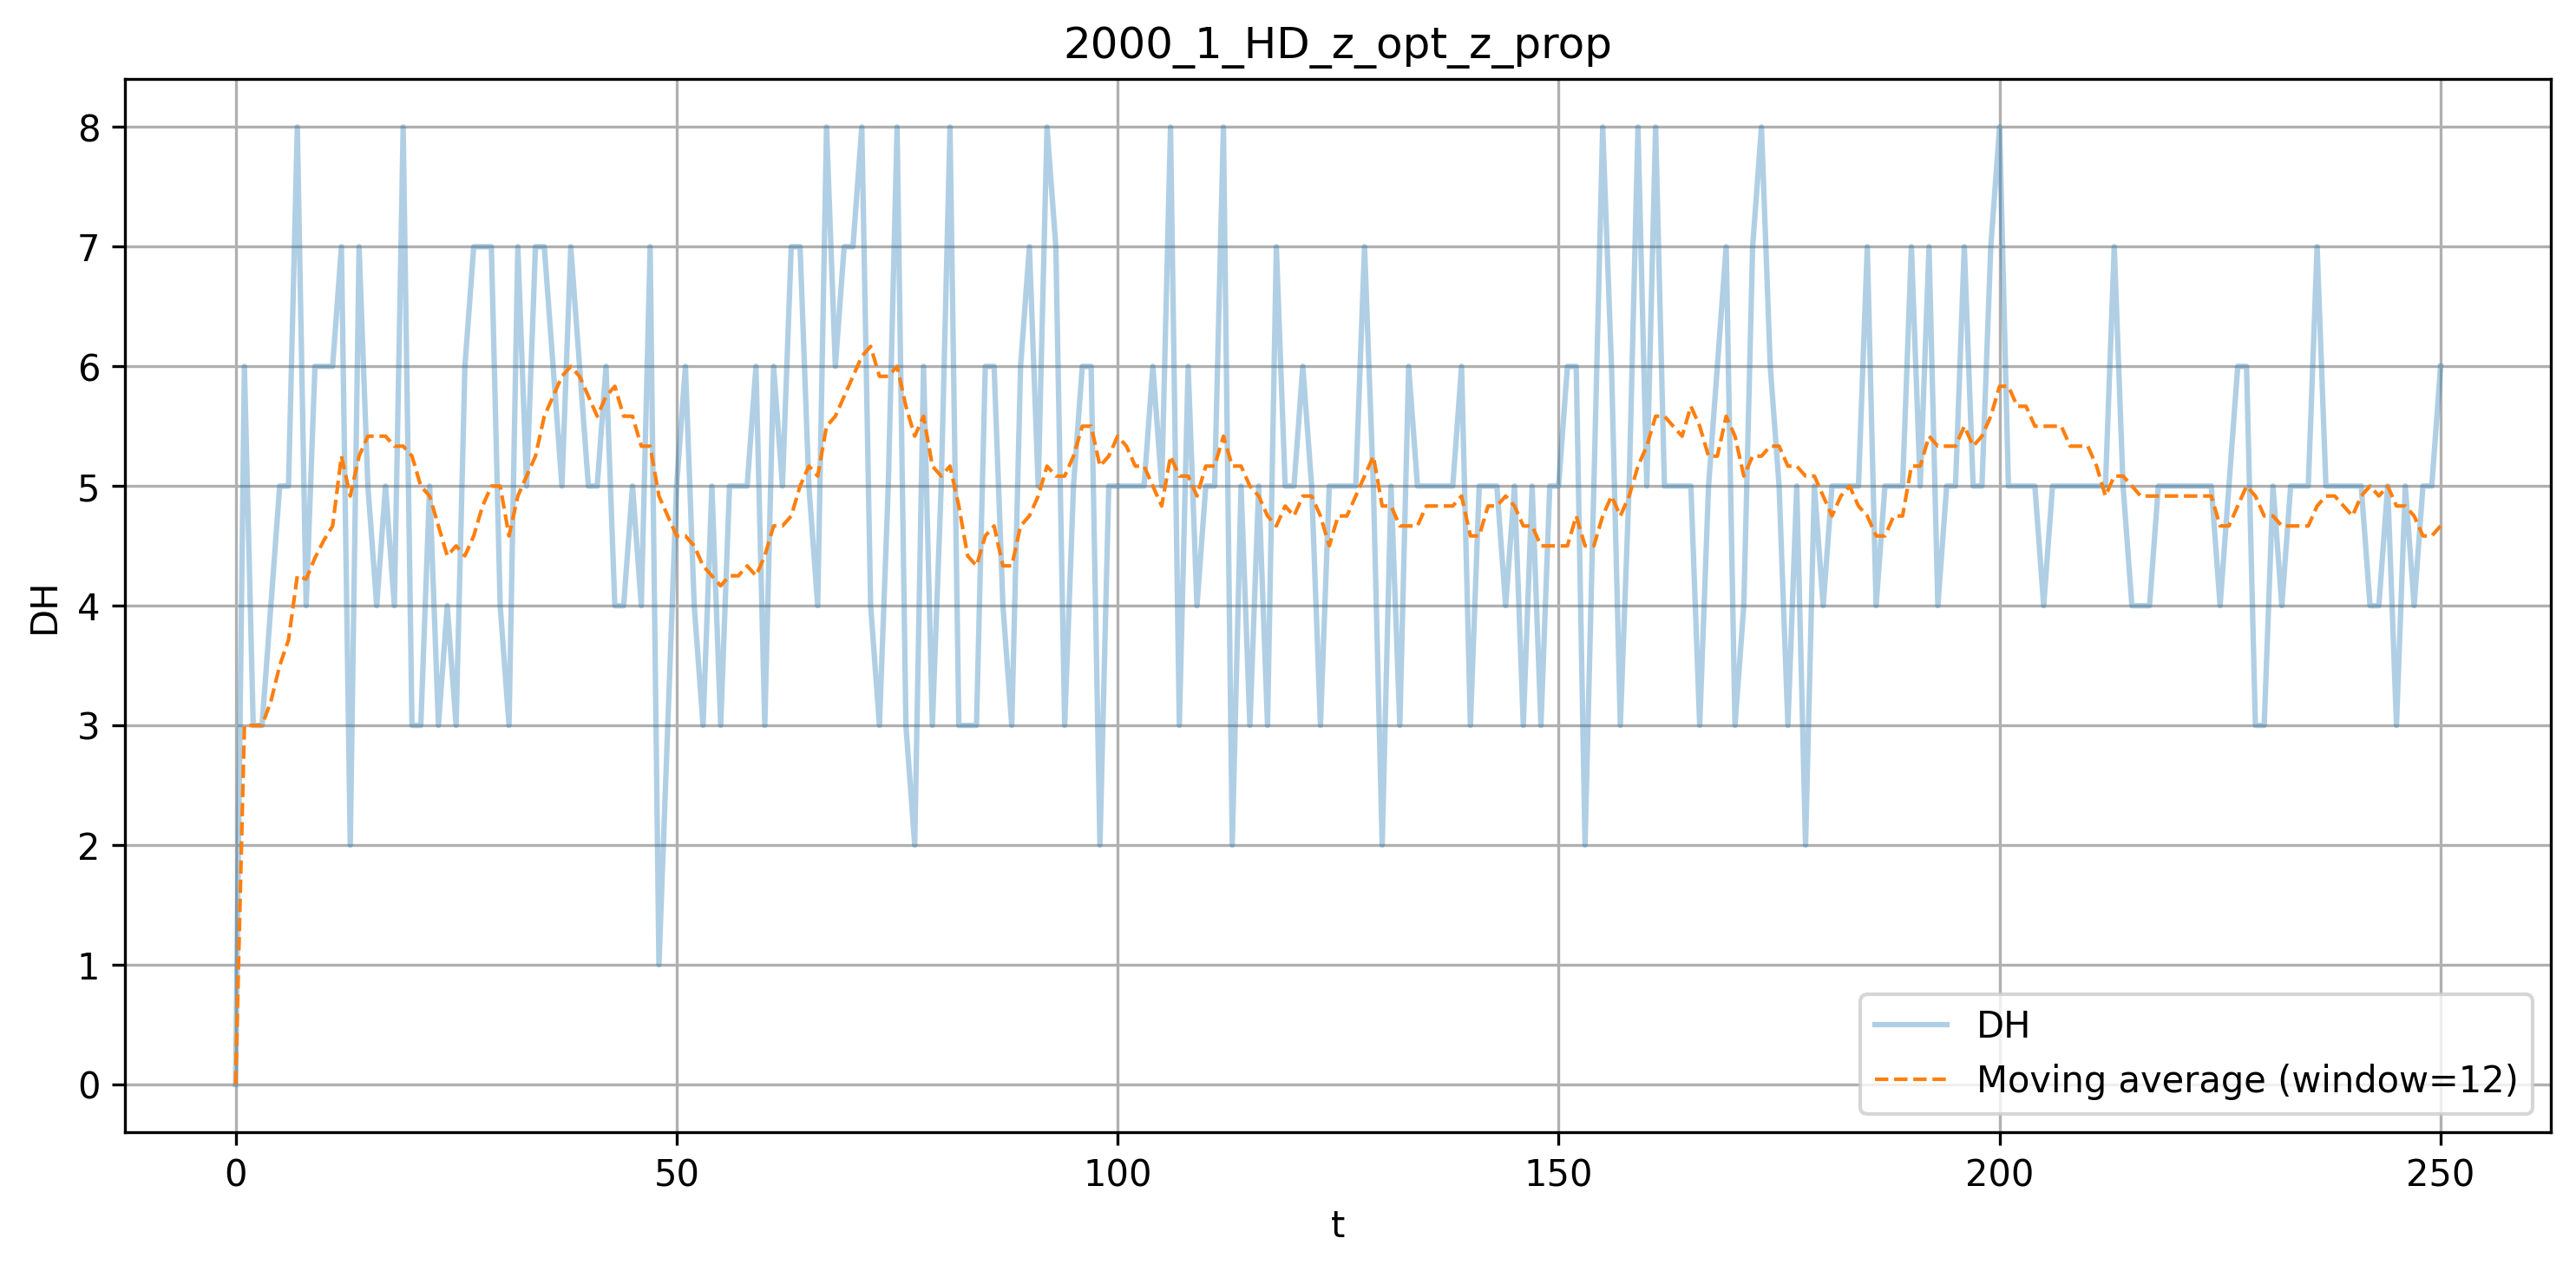
\includegraphics[width=\linewidth]{../Quantum-Annealing-for-solving-QUBO-Problems/test/Lambda_dinamico/ksp_1/lambda_div_3/2000_1_HD_z_opt_z_prop.png}
    \caption{\(d_H(z_{opt}, z_t)\) con \(\lambda_2\)}
    \label{fig:hd-zopt-zprop-lambda2}
\end{subfigure}

\vspace{0.35cm}

\begin{subfigure}{0.495\textwidth}
    \centering
    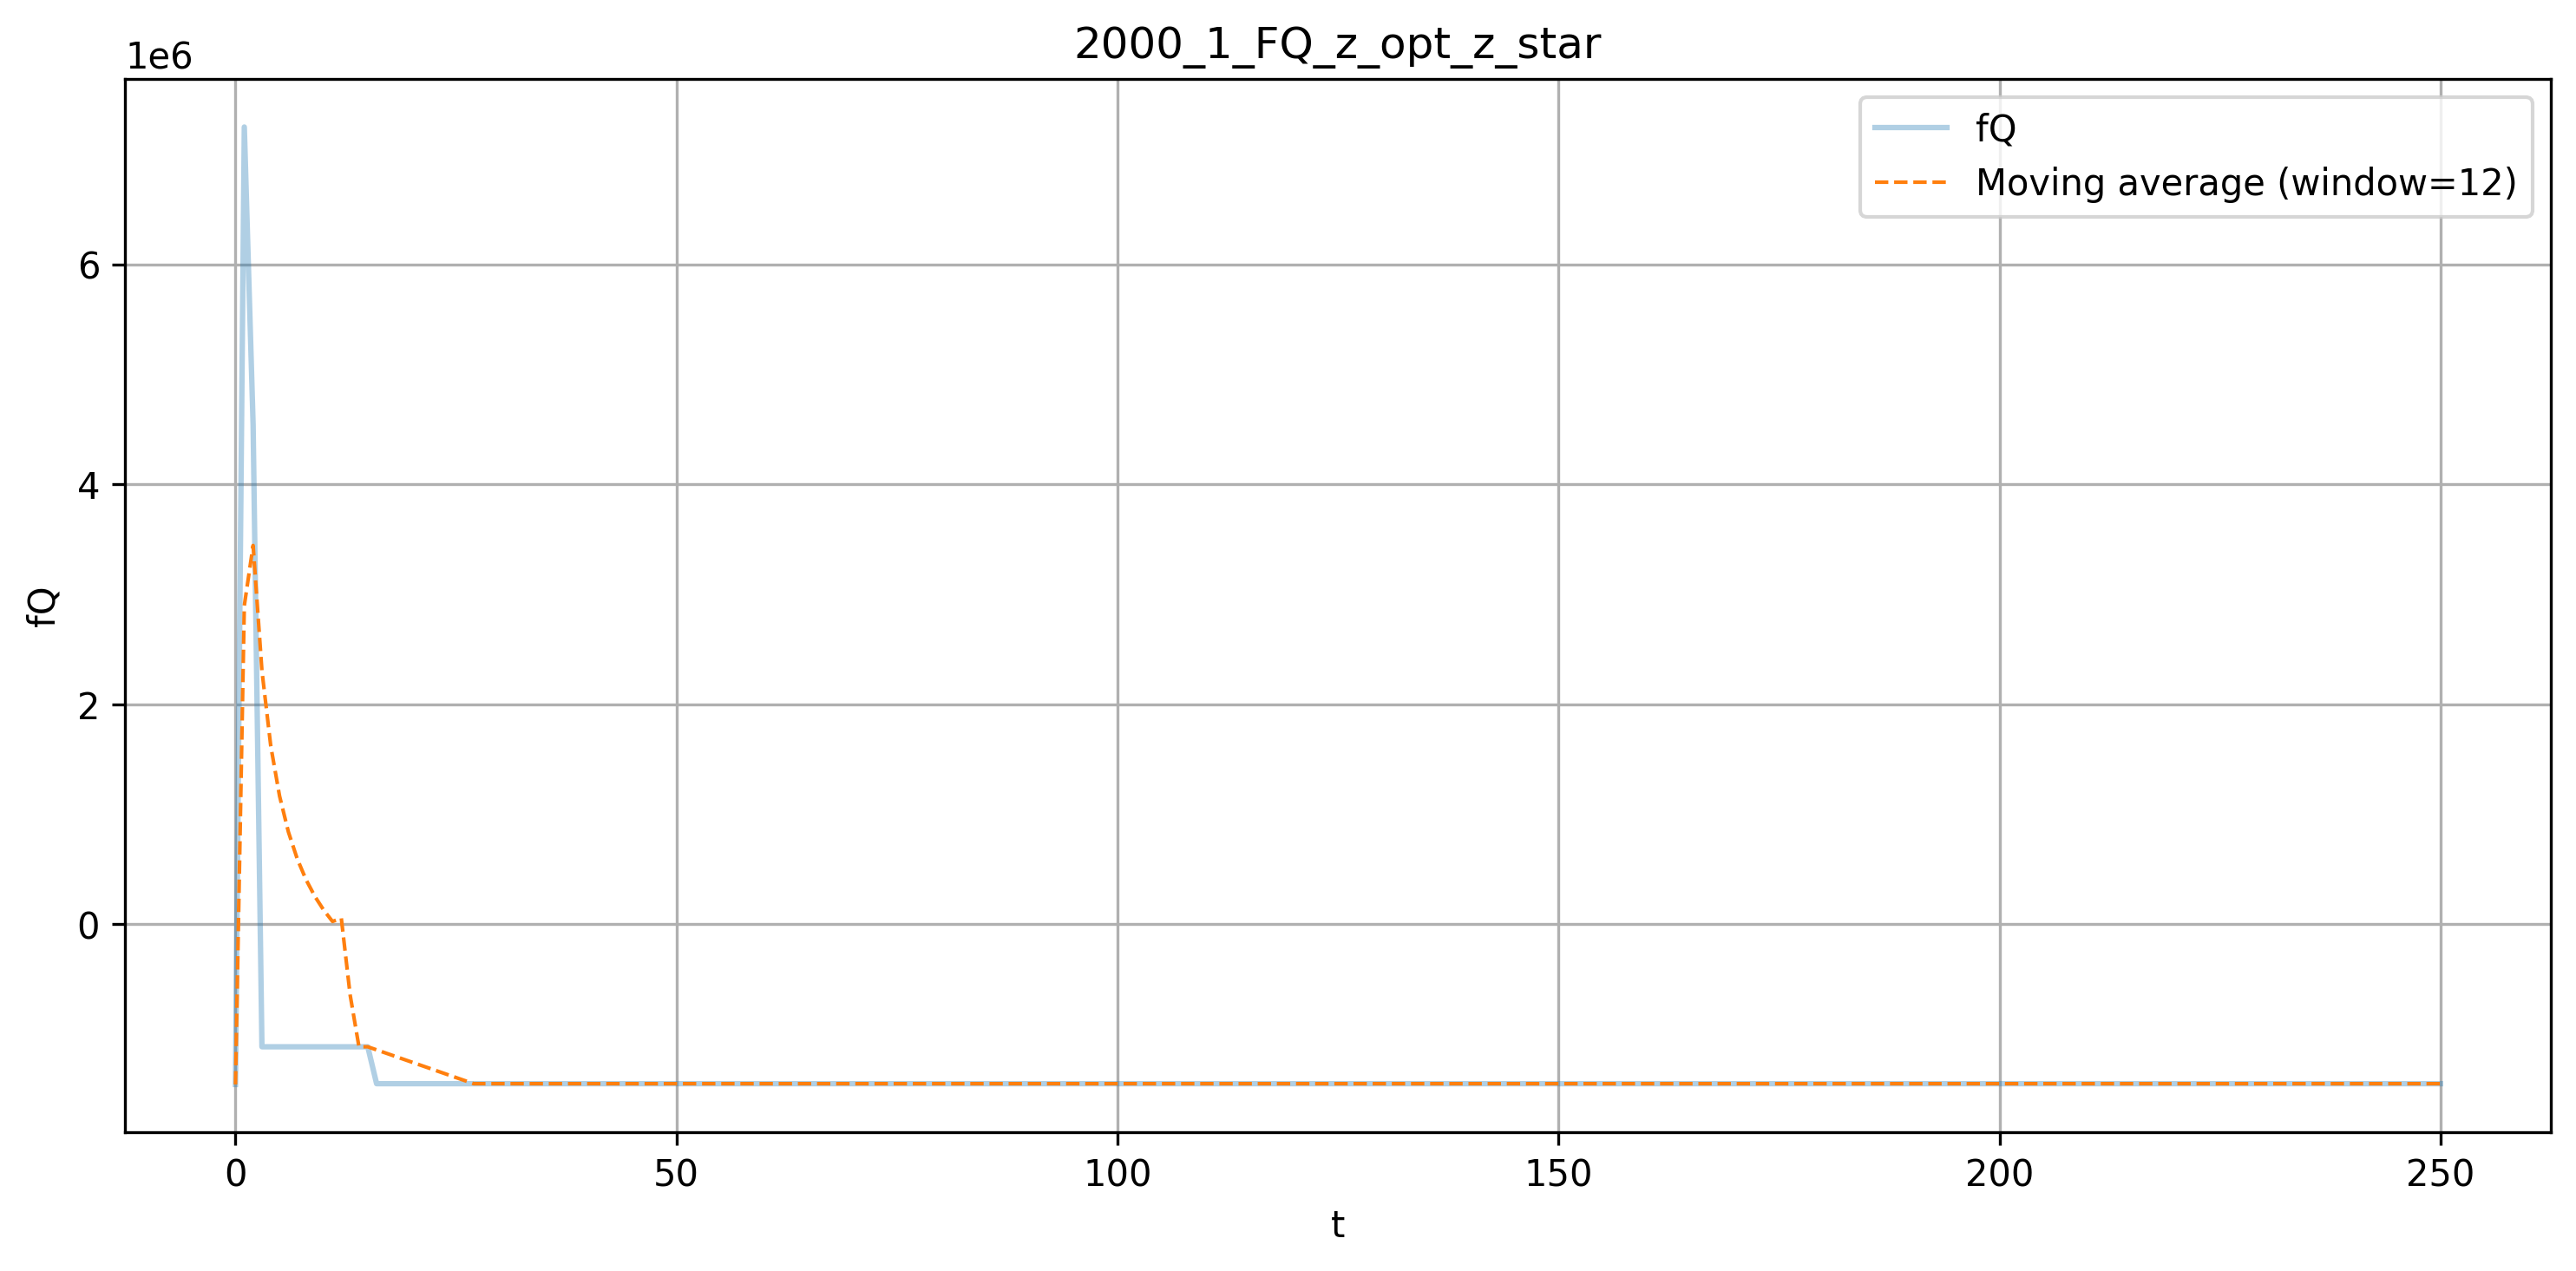
\includegraphics[width=\linewidth]{../Quantum-Annealing-for-solving-QUBO-Problems/test/Lambda_dinamico/ksp_1/lambda_div_3/2000_1_FQ_z_opt_z_star.png}
    \caption{\(f_Q(z_\star)\) con \(\lambda_2\)}
    \label{fig:fQ-zstar-lambda2}
\end{subfigure}
\hfill
\begin{subfigure}{0.495\textwidth}
    \centering
    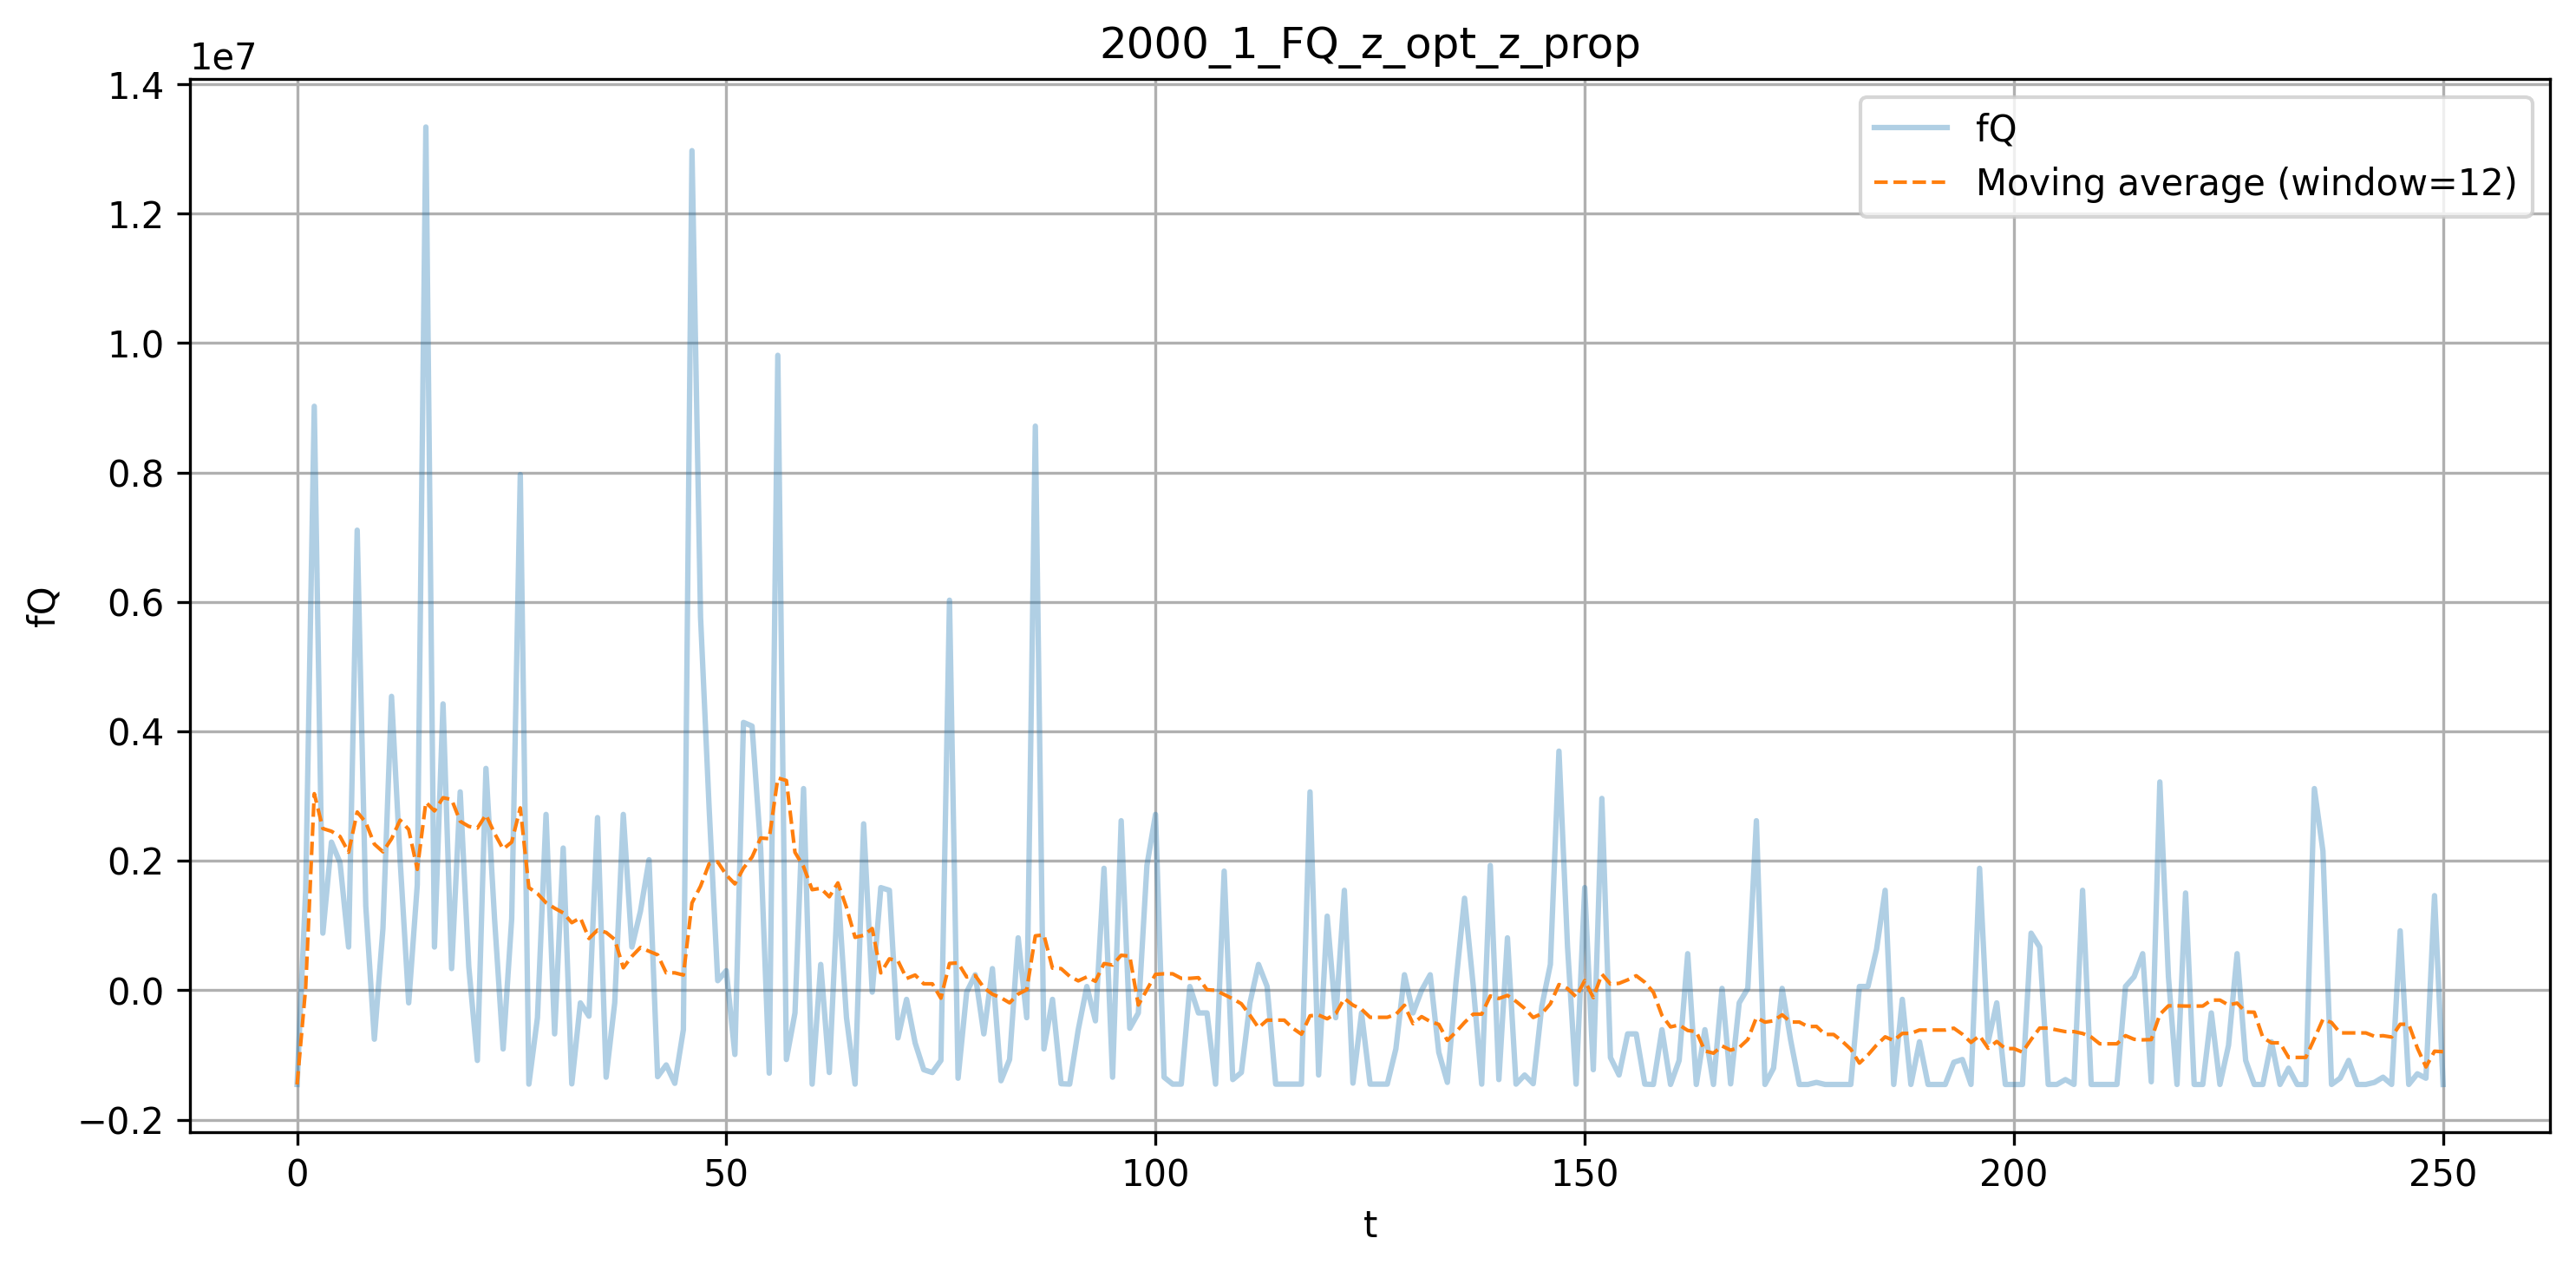
\includegraphics[width=\linewidth]{../Quantum-Annealing-for-solving-QUBO-Problems/test/Lambda_dinamico/ksp_1/lambda_div_3/2000_1_FQ_z_opt_z_prop.png}
    \caption{\(f_Q(z_t)\) con \(\lambda_2\)}
    \label{fig:fQ-zt-lambda2}
\end{subfigure}
\label{fig:confronto-hamming-ksp12}
\end{figure}

\begin{figure}[H]
\centering
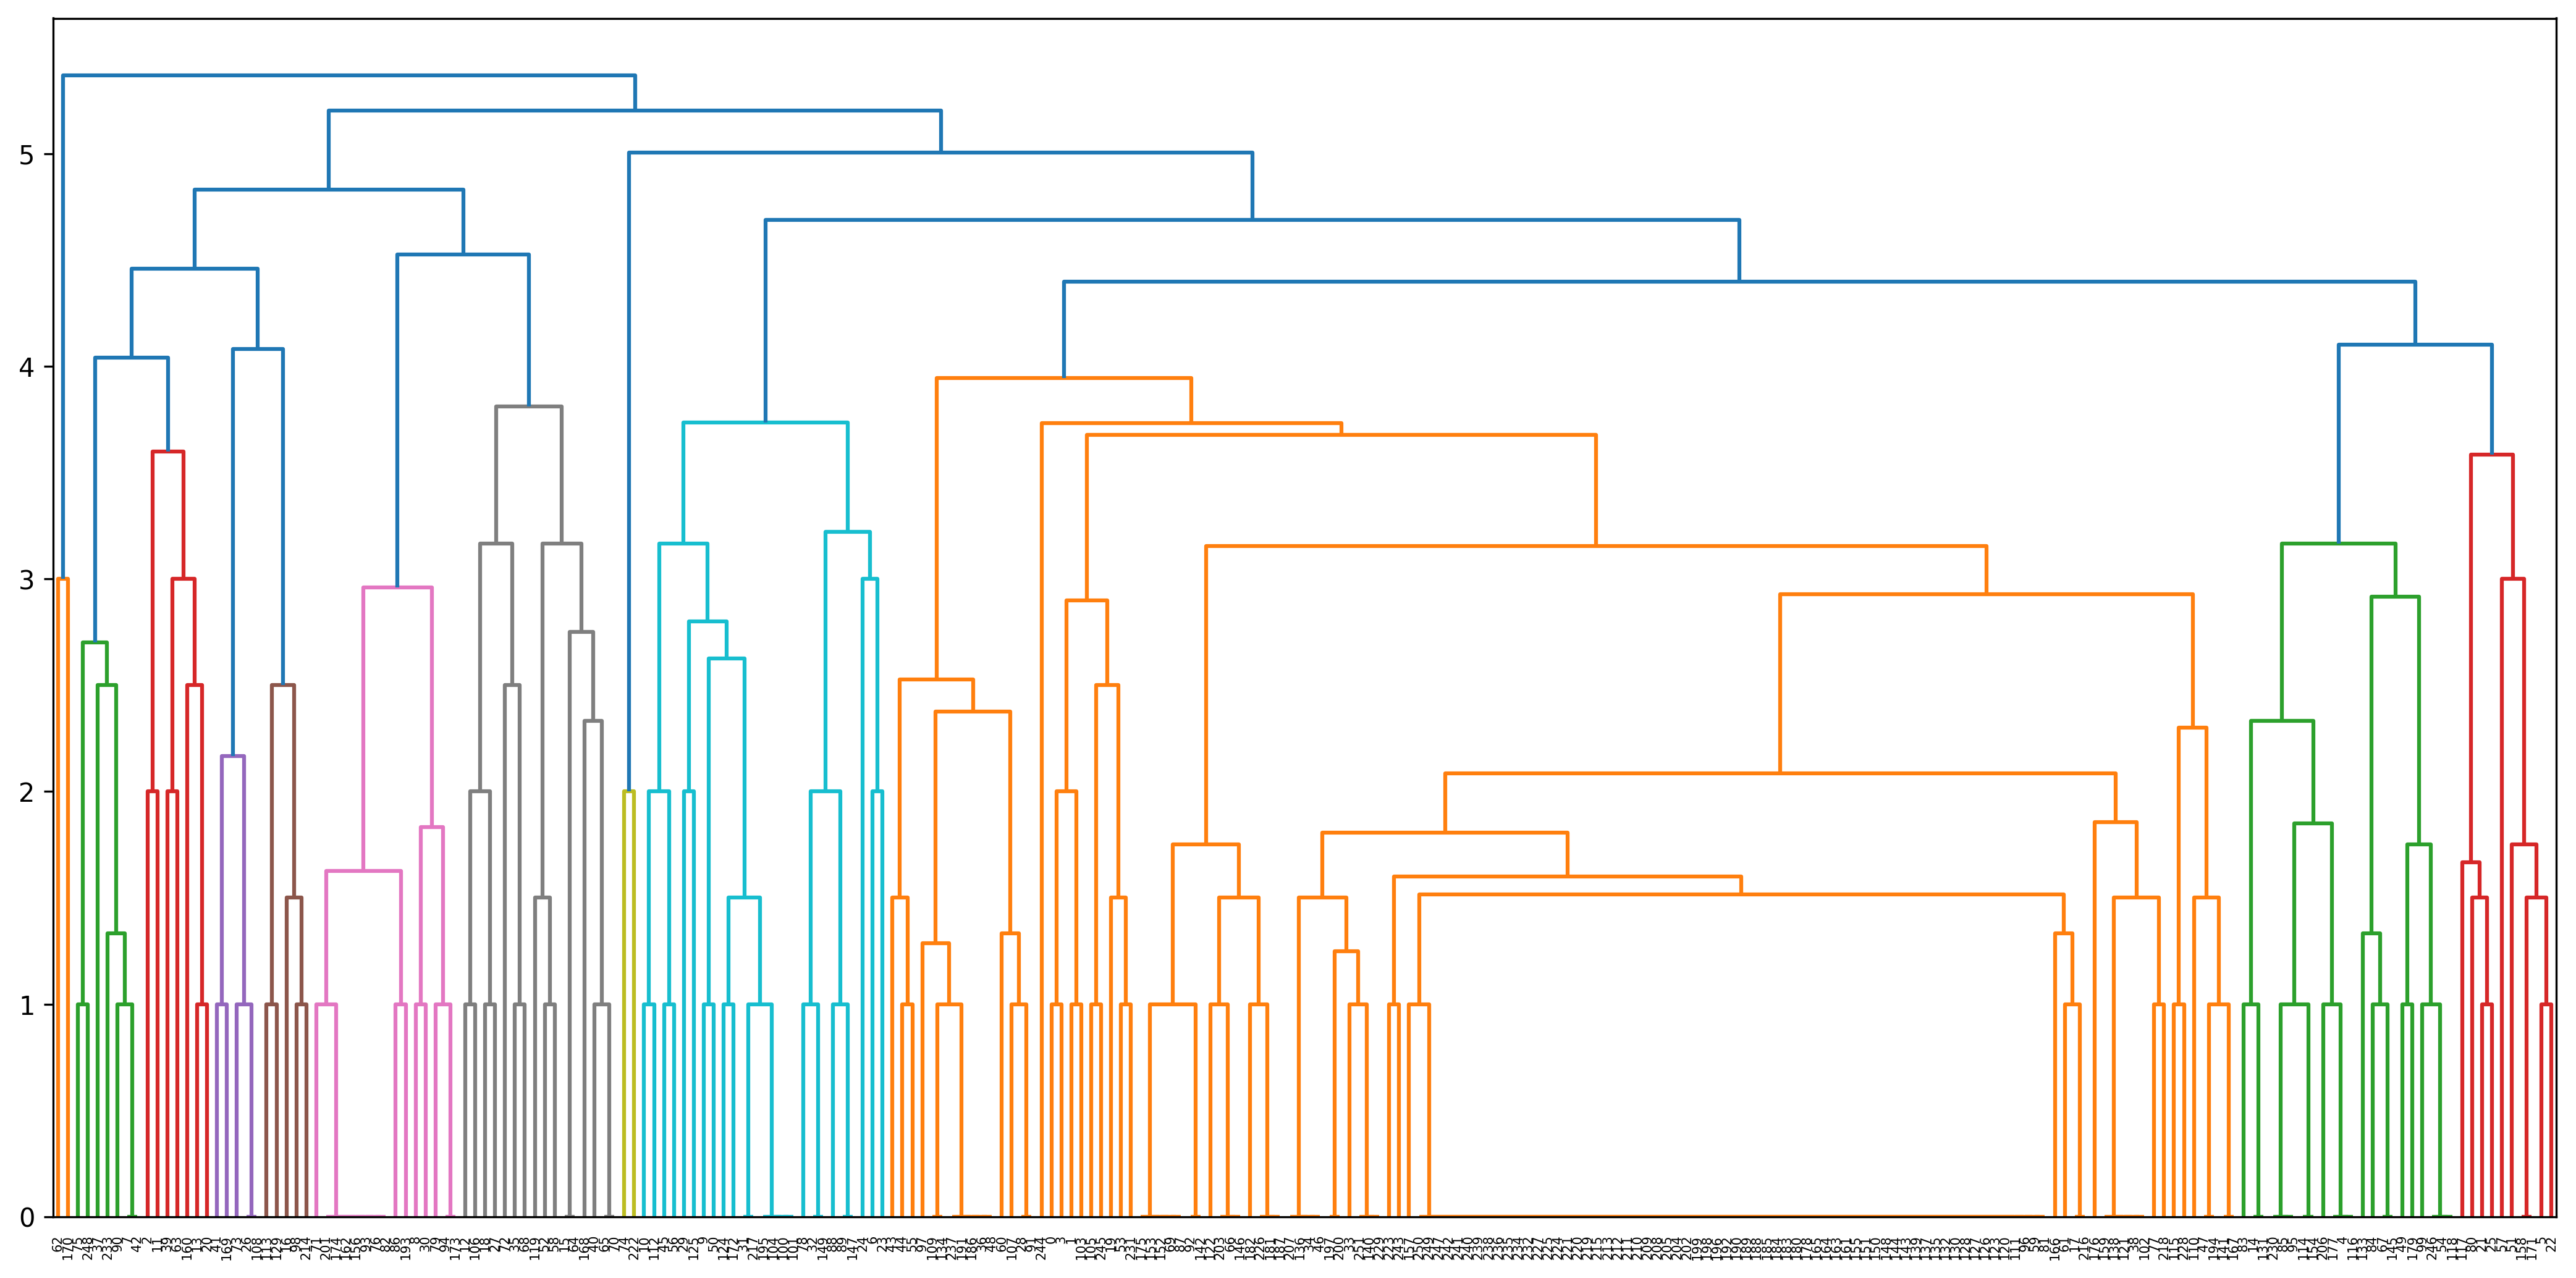
\includegraphics[width=\linewidth]{../Quantum-Annealing-for-solving-QUBO-Problems/test/Lambda_dinamico/ksp_1/lambda_div_3/dendrogram_2000_1.png}
\caption{Agglomerative Clustering Dendogram}
\label{fig:AgglomerativeClustering-ksp1}
\end{figure}

\clearpage
\subsection{ksp\_3}

\begin{table}[h]
\centering
\begin{tabular}{lcc}
\hline
\textbf{Metrica} & \(\lambda_1\) & \(\lambda_2\) \\
\hline
Numero cluster & 37 & 32 \\
Dimensione cluster massimo & 61 & 107 \\
Cluster z best & [2, 43] & [2, 107] \\
Single clusters & 2 & 2 \\
\(f_Q\) medoid & 37513.44 & 777361961.67 \\
Profit medoid & 2628 & 3030 \\
Weight medoid & 1836 & 1225 \\
\hline
\(f_Q\) Min Found QALS & 943.84 & 777361961.67 \\
Profit Found QALS & 3484 & 3030 \\
Weight Found QALS & 1149 & 1225 \\
\hline
\(f_Q\) Min Found NO QALS & -9424.80 & -714267662.00 \\
Profit Found NO QALS & 2936 & 2483 \\
Weight Found NO QALS & 560 & 501 \\
\hline
\end{tabular}
\caption{Confronto dei risultati ottenuti con QALS e senza QALS.}
\label{tab:confronto-qals-noqals-ksp}
\end{table}

\begin{figure}[H]
\centering
\begin{subfigure}{0.495\textwidth}
    \centering
    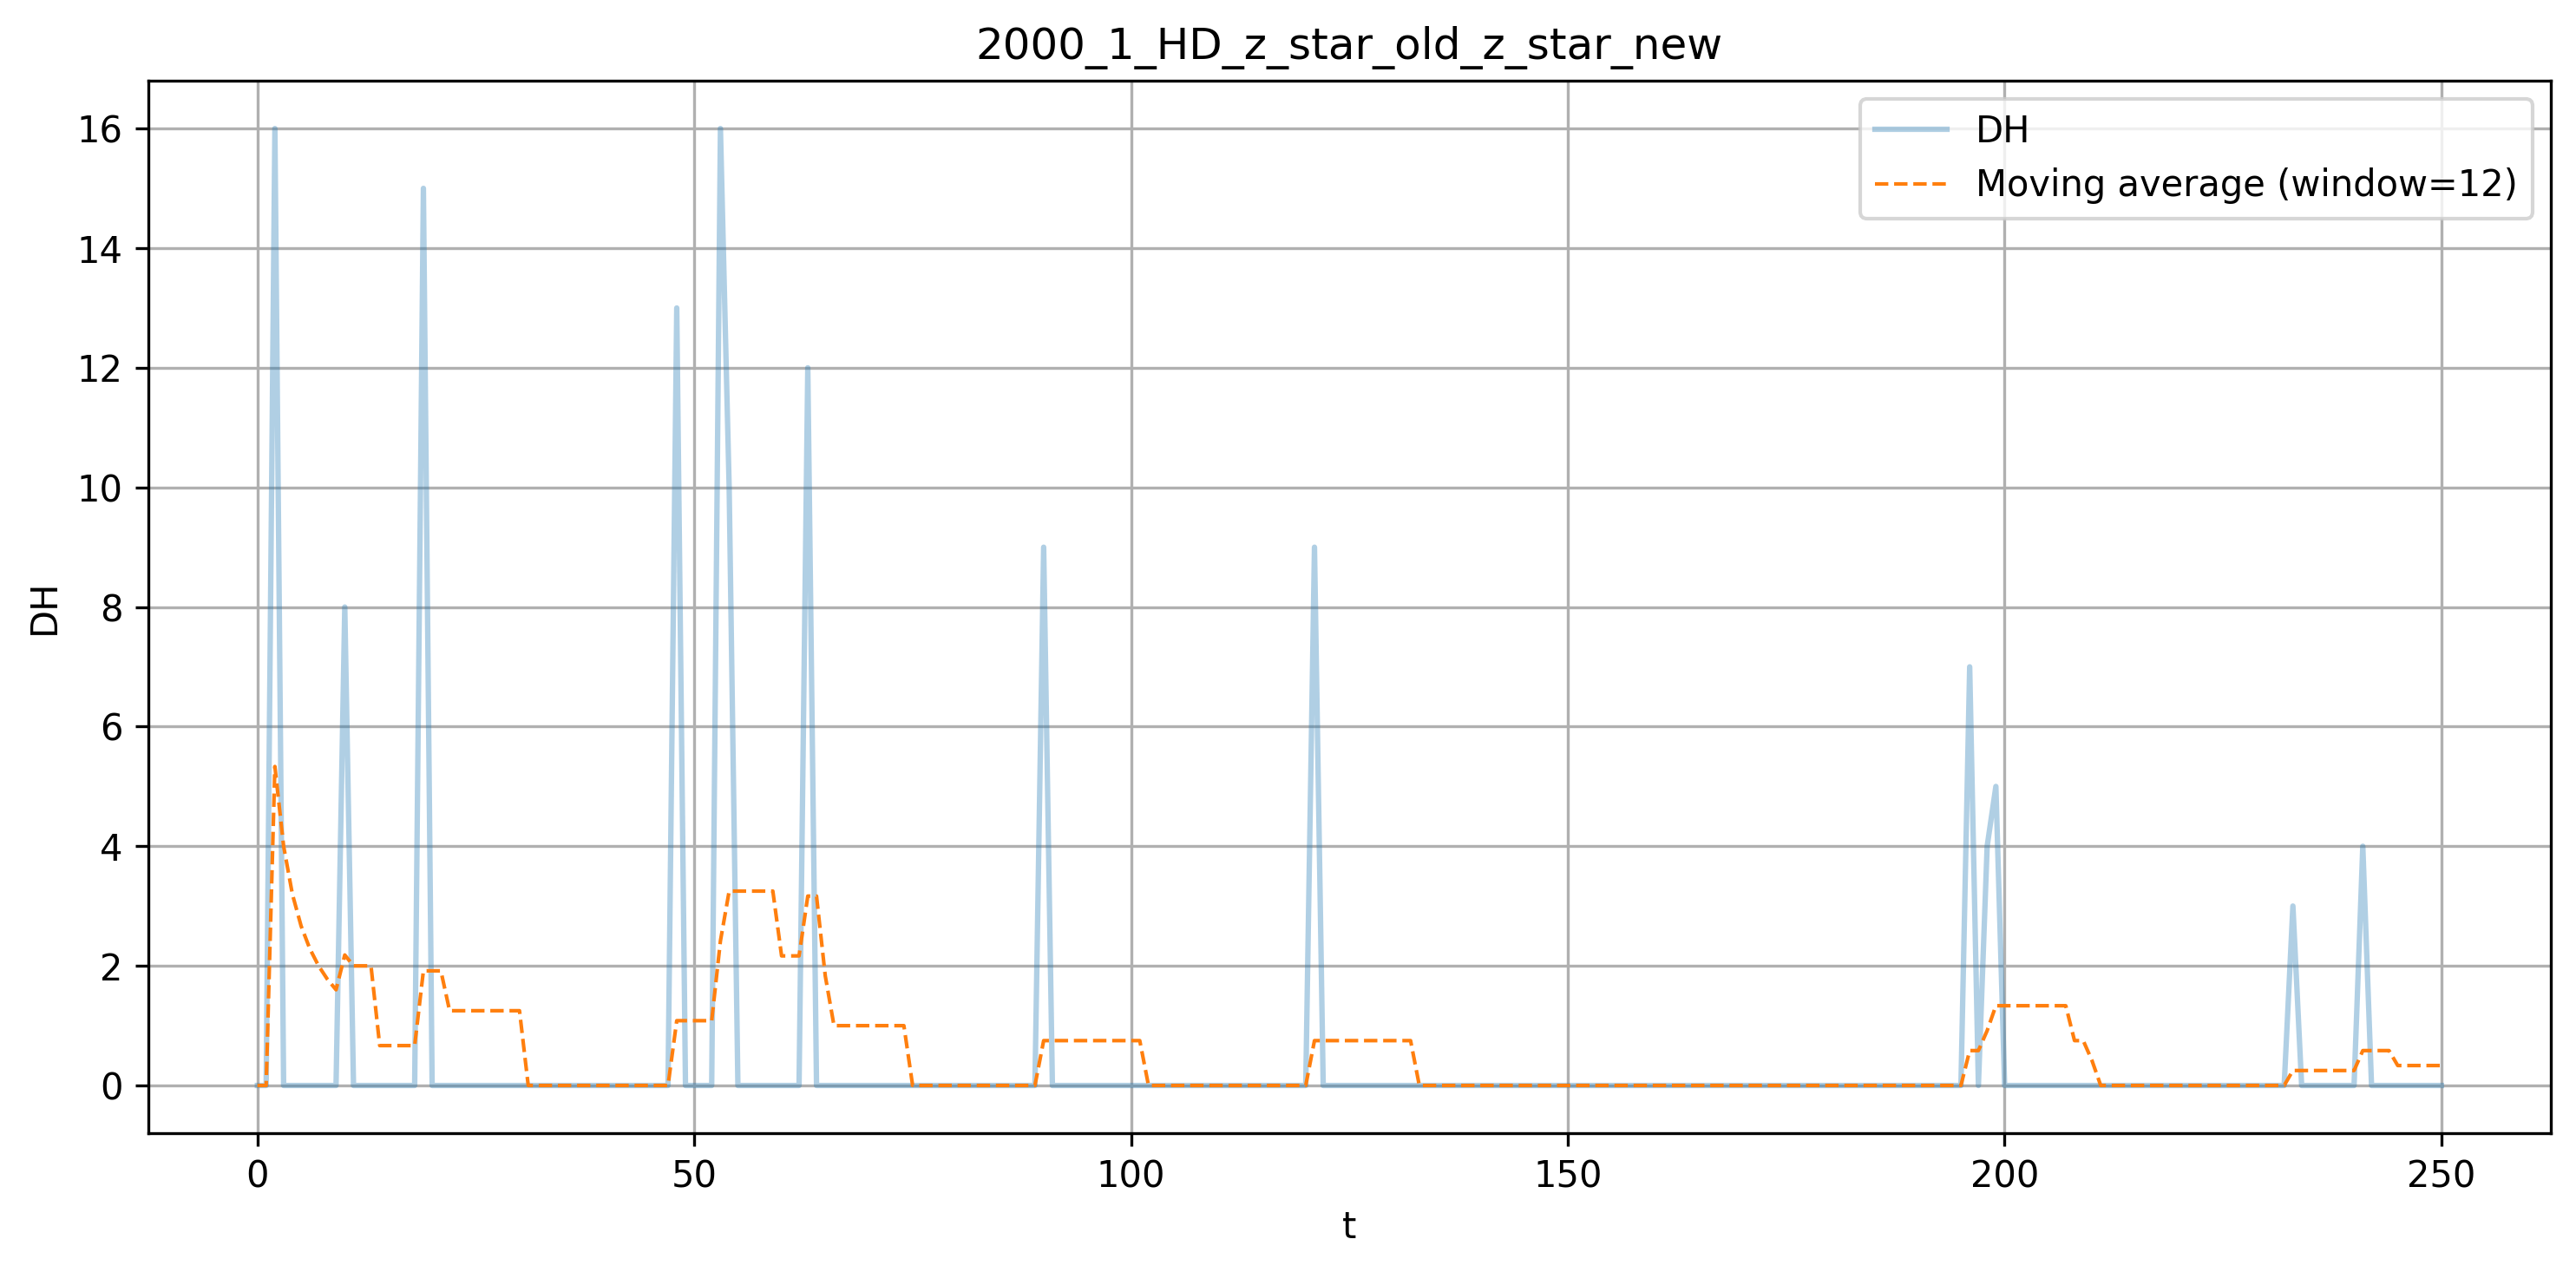
\includegraphics[width=\linewidth]{../Quantum-Annealing-for-solving-QUBO-Problems/test/Lambda_dinamico/ksp_3/lambda_650_dot_C/2000_1_HD_z_star_old_z_star_new.png}
    \caption{\(d_H(z_\star^{old}, z_\star^{new})\) con \(\lambda_1\)}
    \label{fig:hd-zstarold-zstarnew-lambda1}
\end{subfigure}
\hfill
\begin{subfigure}{0.495\textwidth}
    \centering
    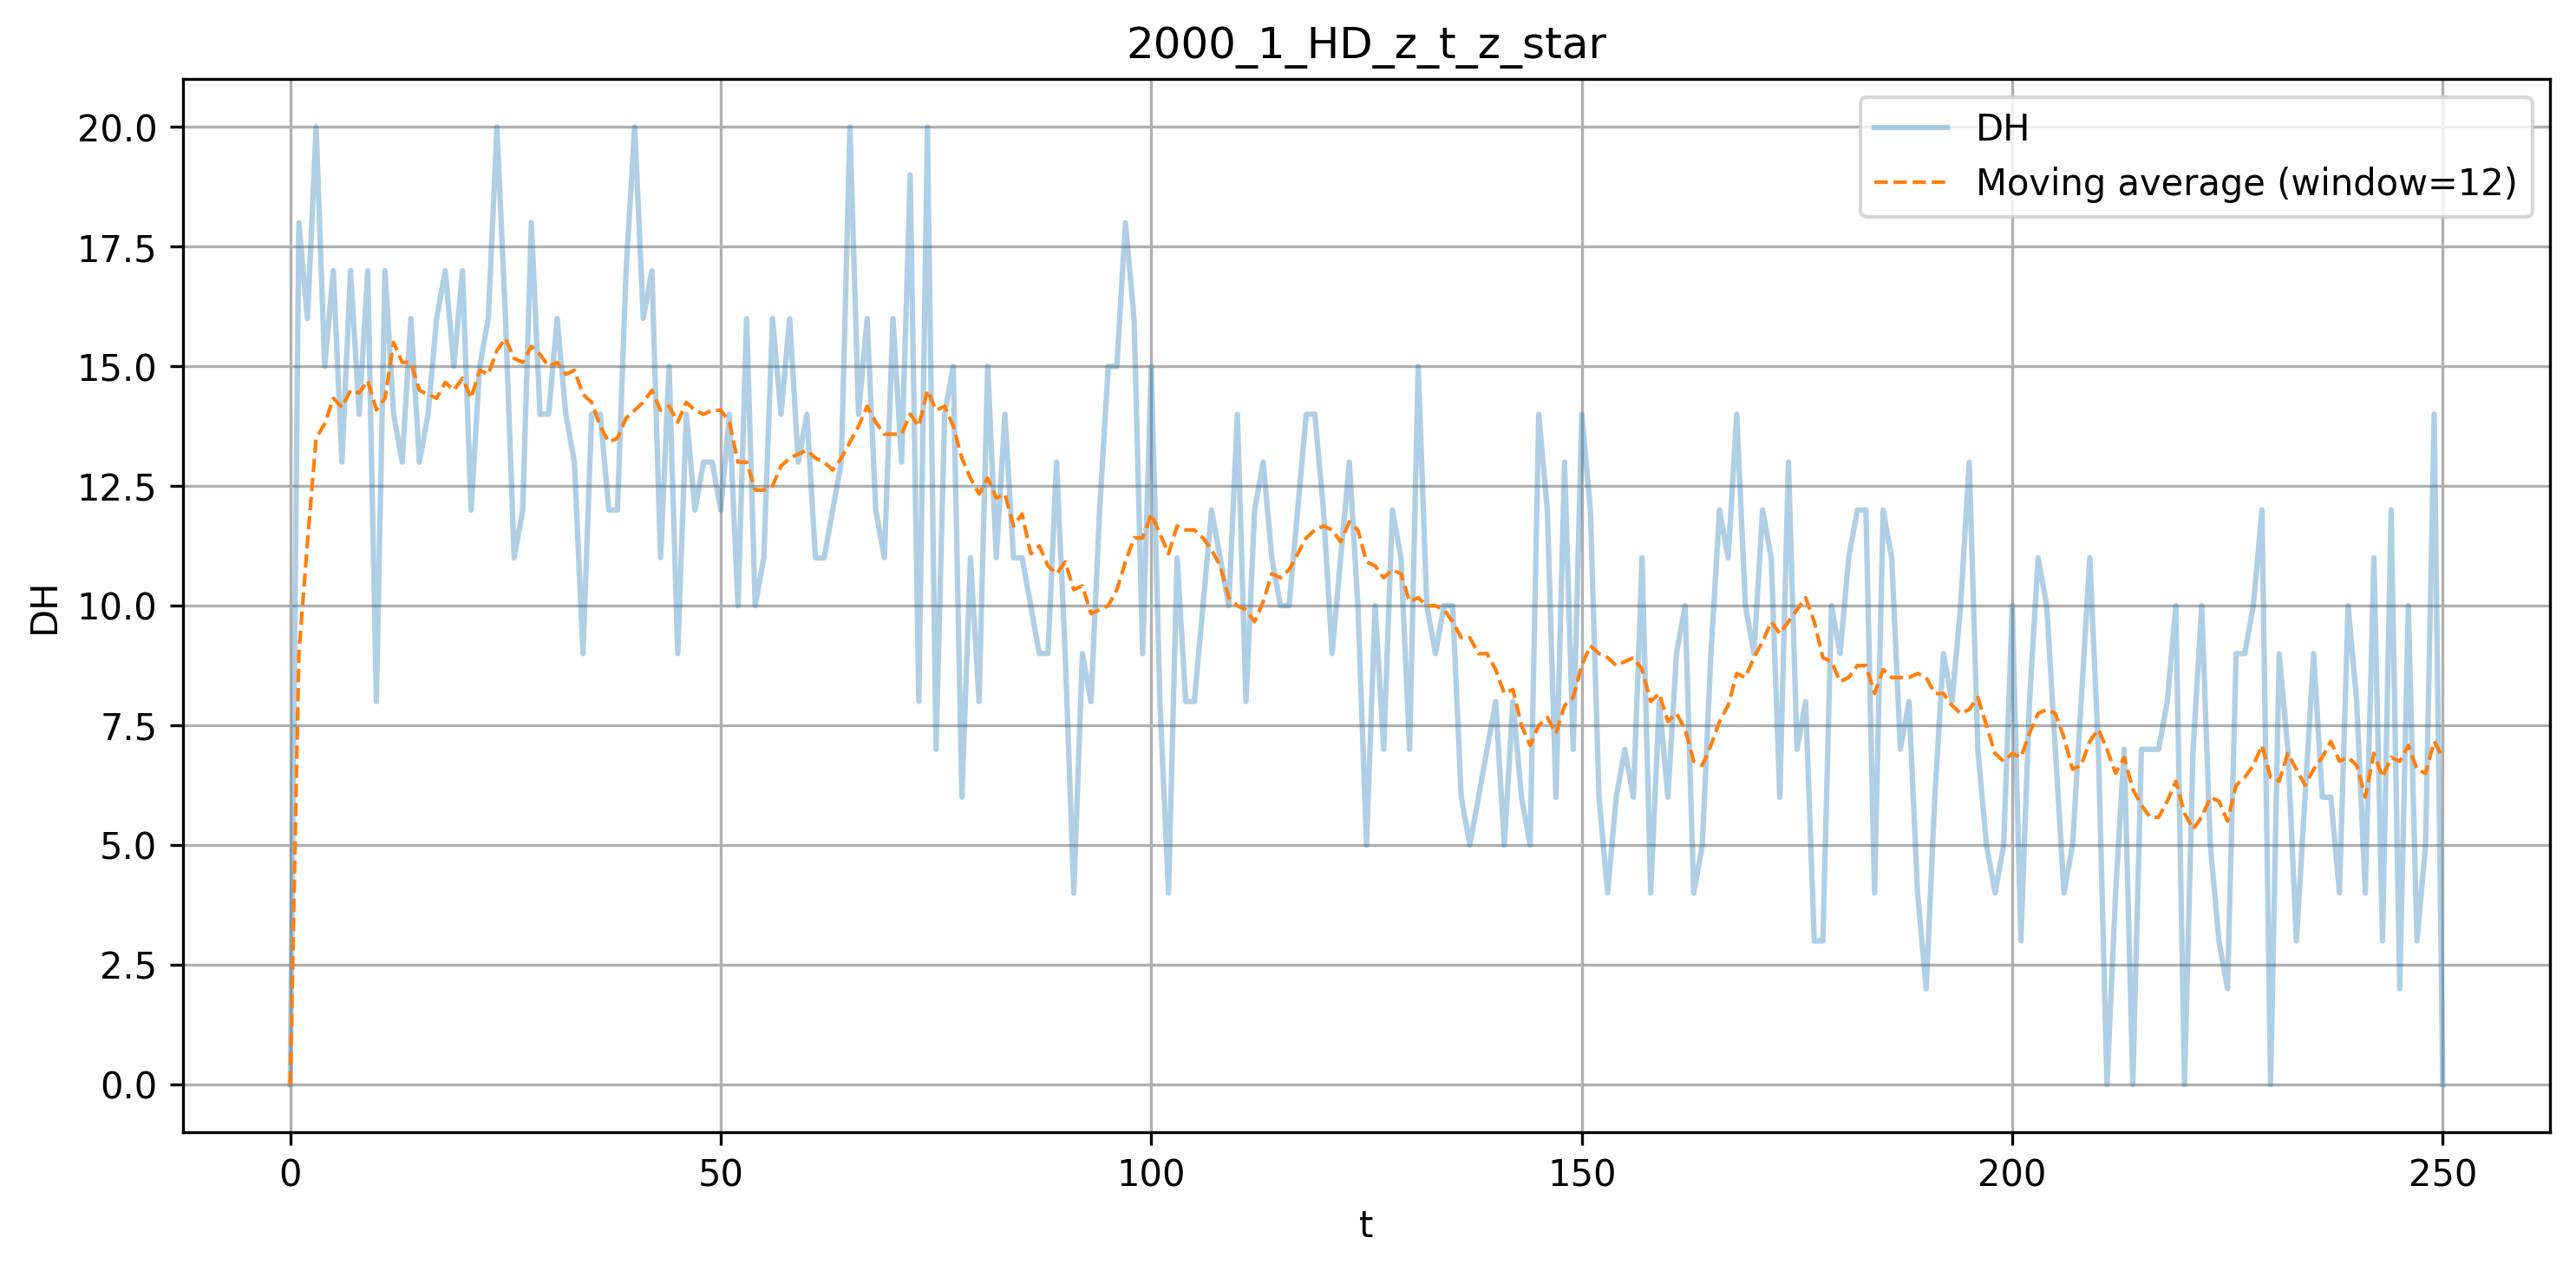
\includegraphics[width=\linewidth]{../Quantum-Annealing-for-solving-QUBO-Problems/test/Lambda_dinamico/ksp_3/lambda_650_dot_C/2000_1_HD_z_t_z_star.png}
    \caption{\(d_H(z_t, z_\star)\) con \(\lambda_1\)}
    \label{fig:hd-zt-zstar-lambda1}
\end{subfigure}

\vspace{0.35cm}

\begin{subfigure}{0.495\textwidth}
    \centering
    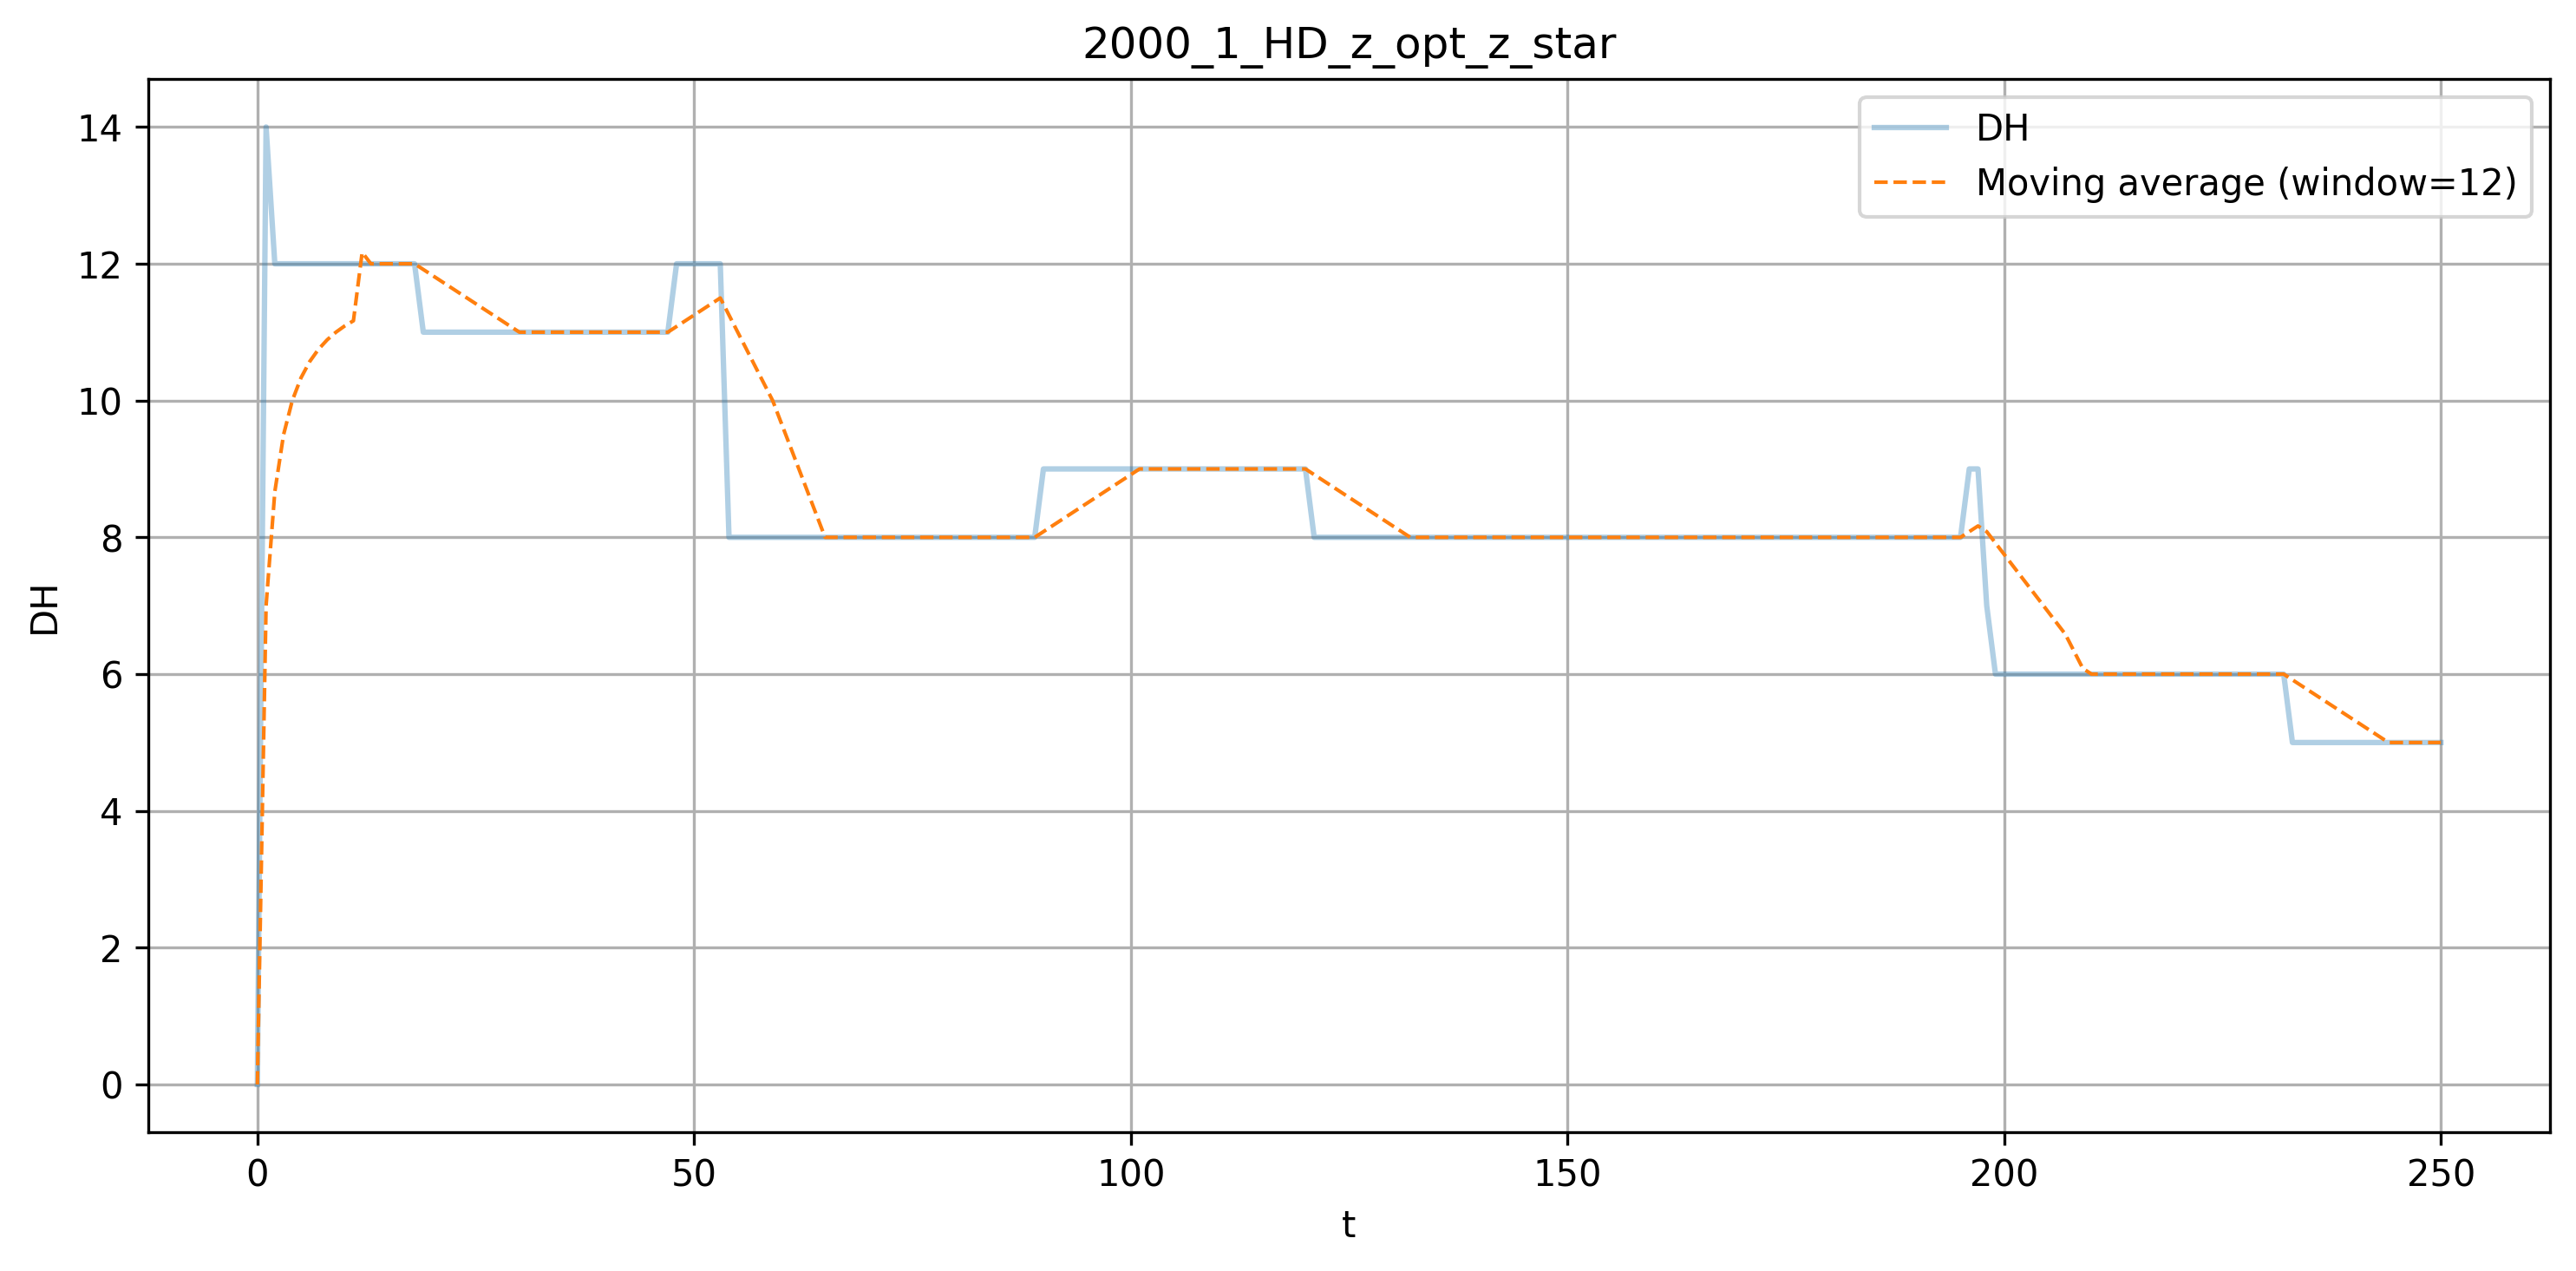
\includegraphics[width=\linewidth]{../Quantum-Annealing-for-solving-QUBO-Problems/test/Lambda_dinamico/ksp_3/lambda_650_dot_C/2000_1_HD_z_opt_z_star.png}
    \caption{\(d_H(z_{opt}, z_\star)\) con \(\lambda_1\)}
    \label{fig:hd-zopt-zstar-lambda1}
\end{subfigure}
\hfill
\begin{subfigure}{0.495\textwidth}
    \centering
    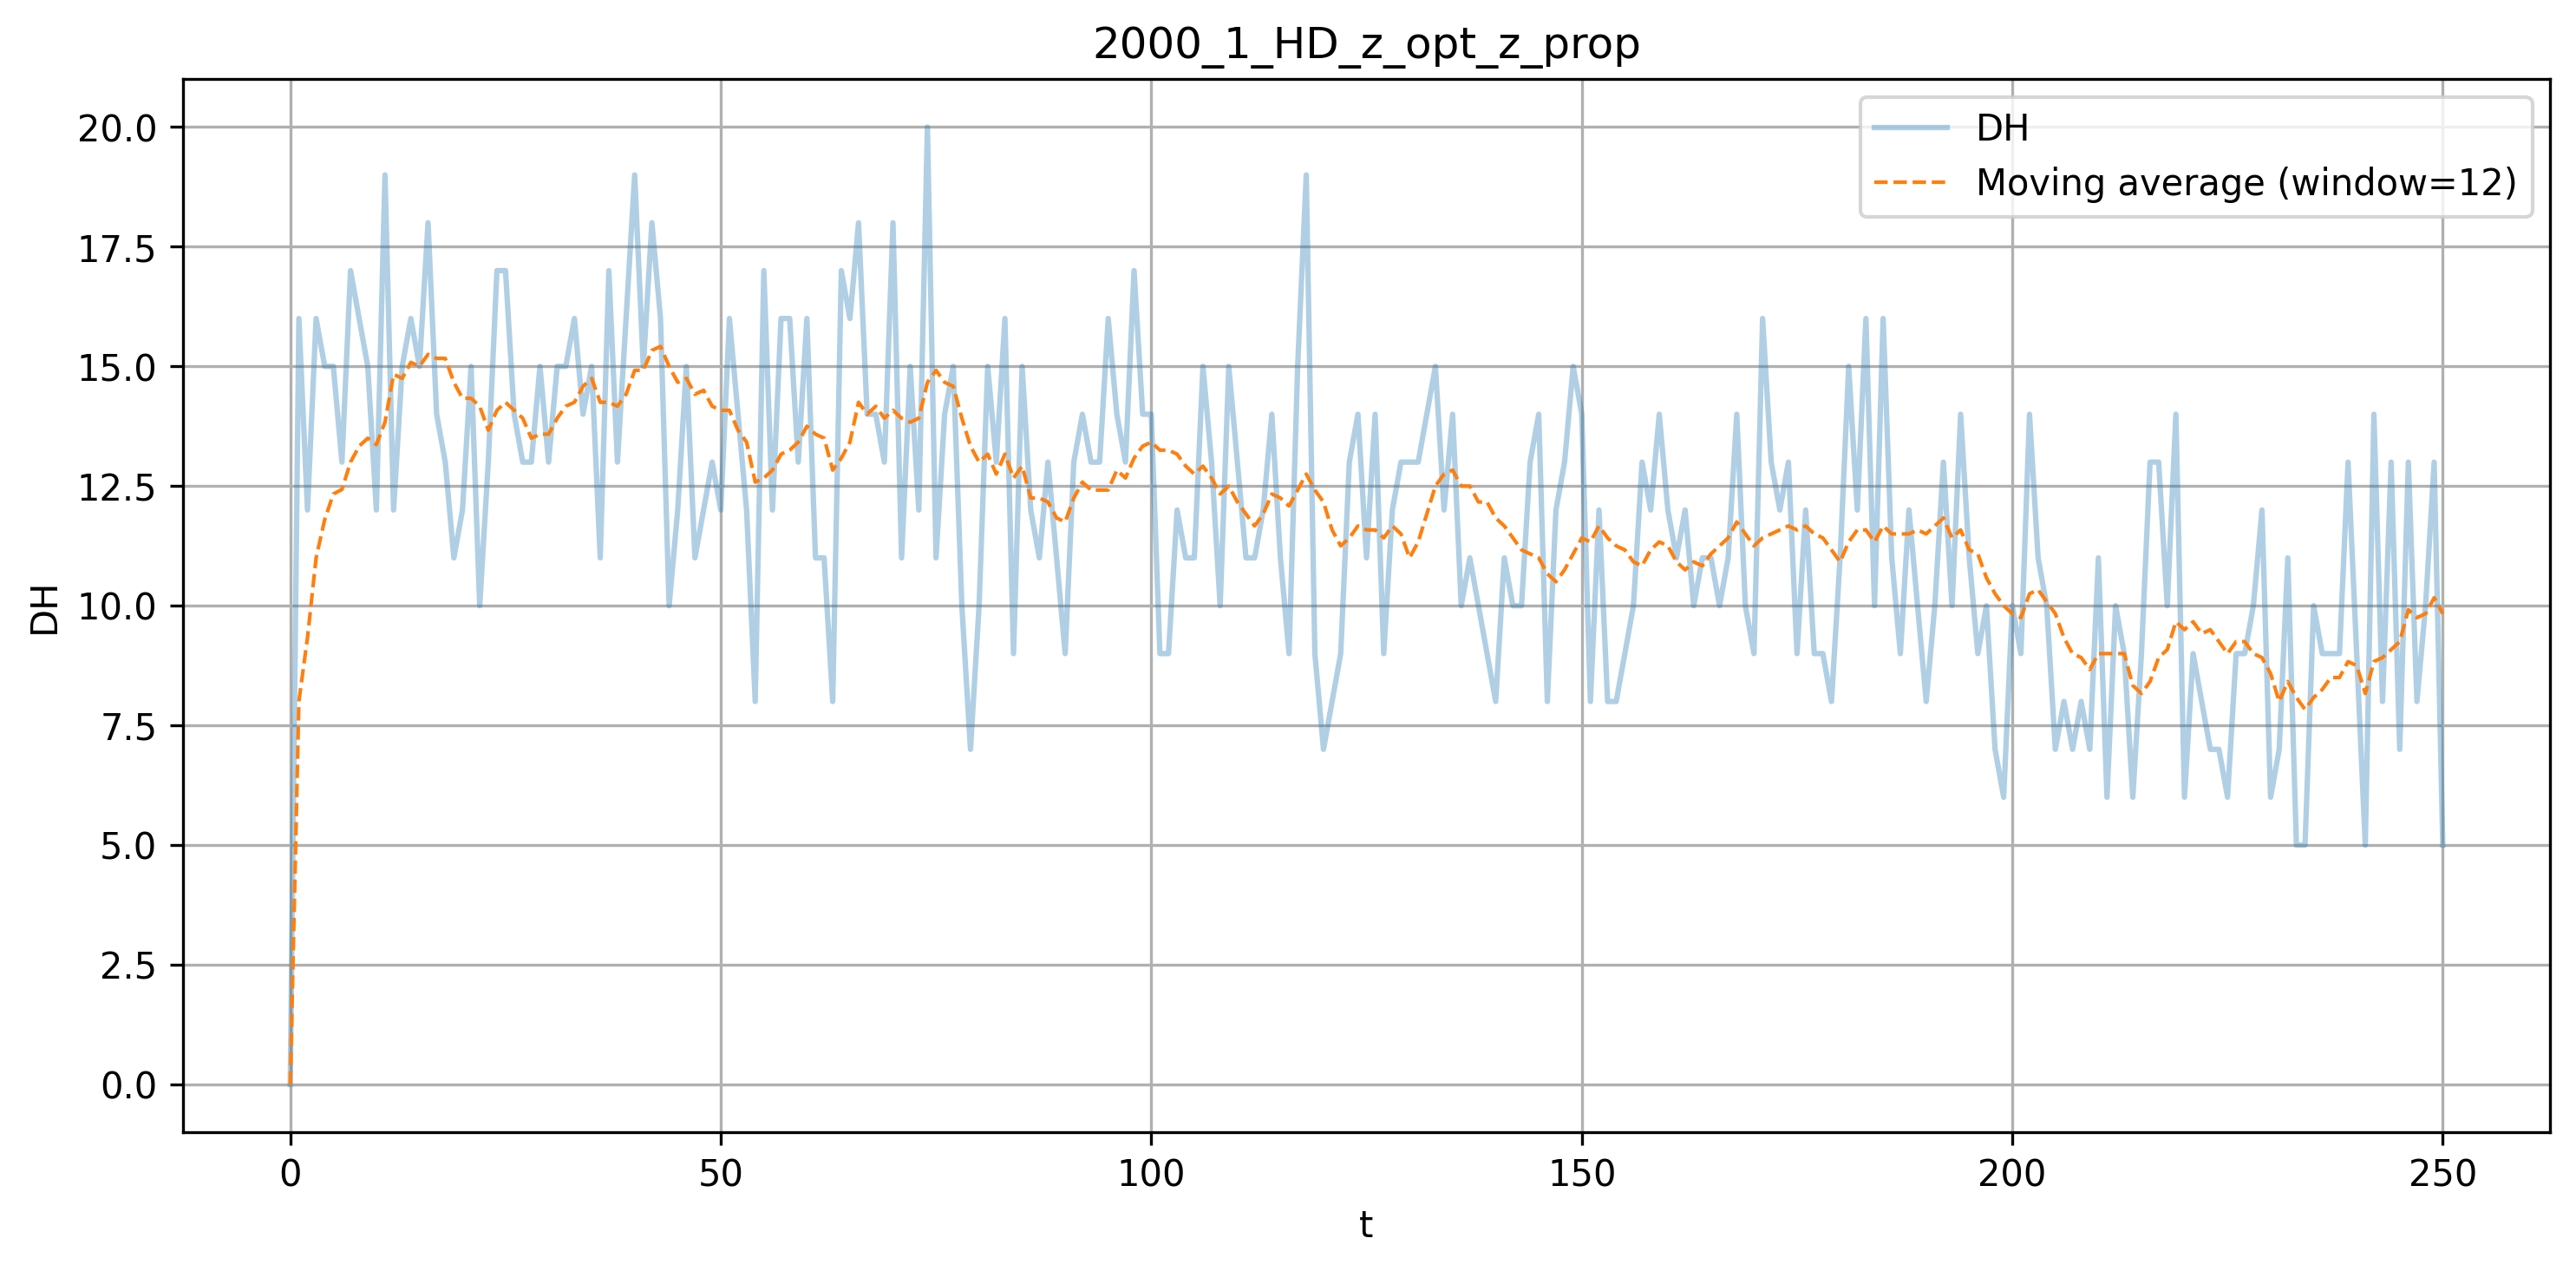
\includegraphics[width=\linewidth]{../Quantum-Annealing-for-solving-QUBO-Problems/test/Lambda_dinamico/ksp_3/lambda_650_dot_C/2000_1_HD_z_opt_z_prop.png}
    \caption{\(d_H(z_{opt}, z_t)\) con \(\lambda_1\)}
    \label{fig:hd-zopt-zt-lambda1}
\end{subfigure}

\vspace{0.35cm}

\begin{subfigure}{0.495\textwidth}
    \centering
    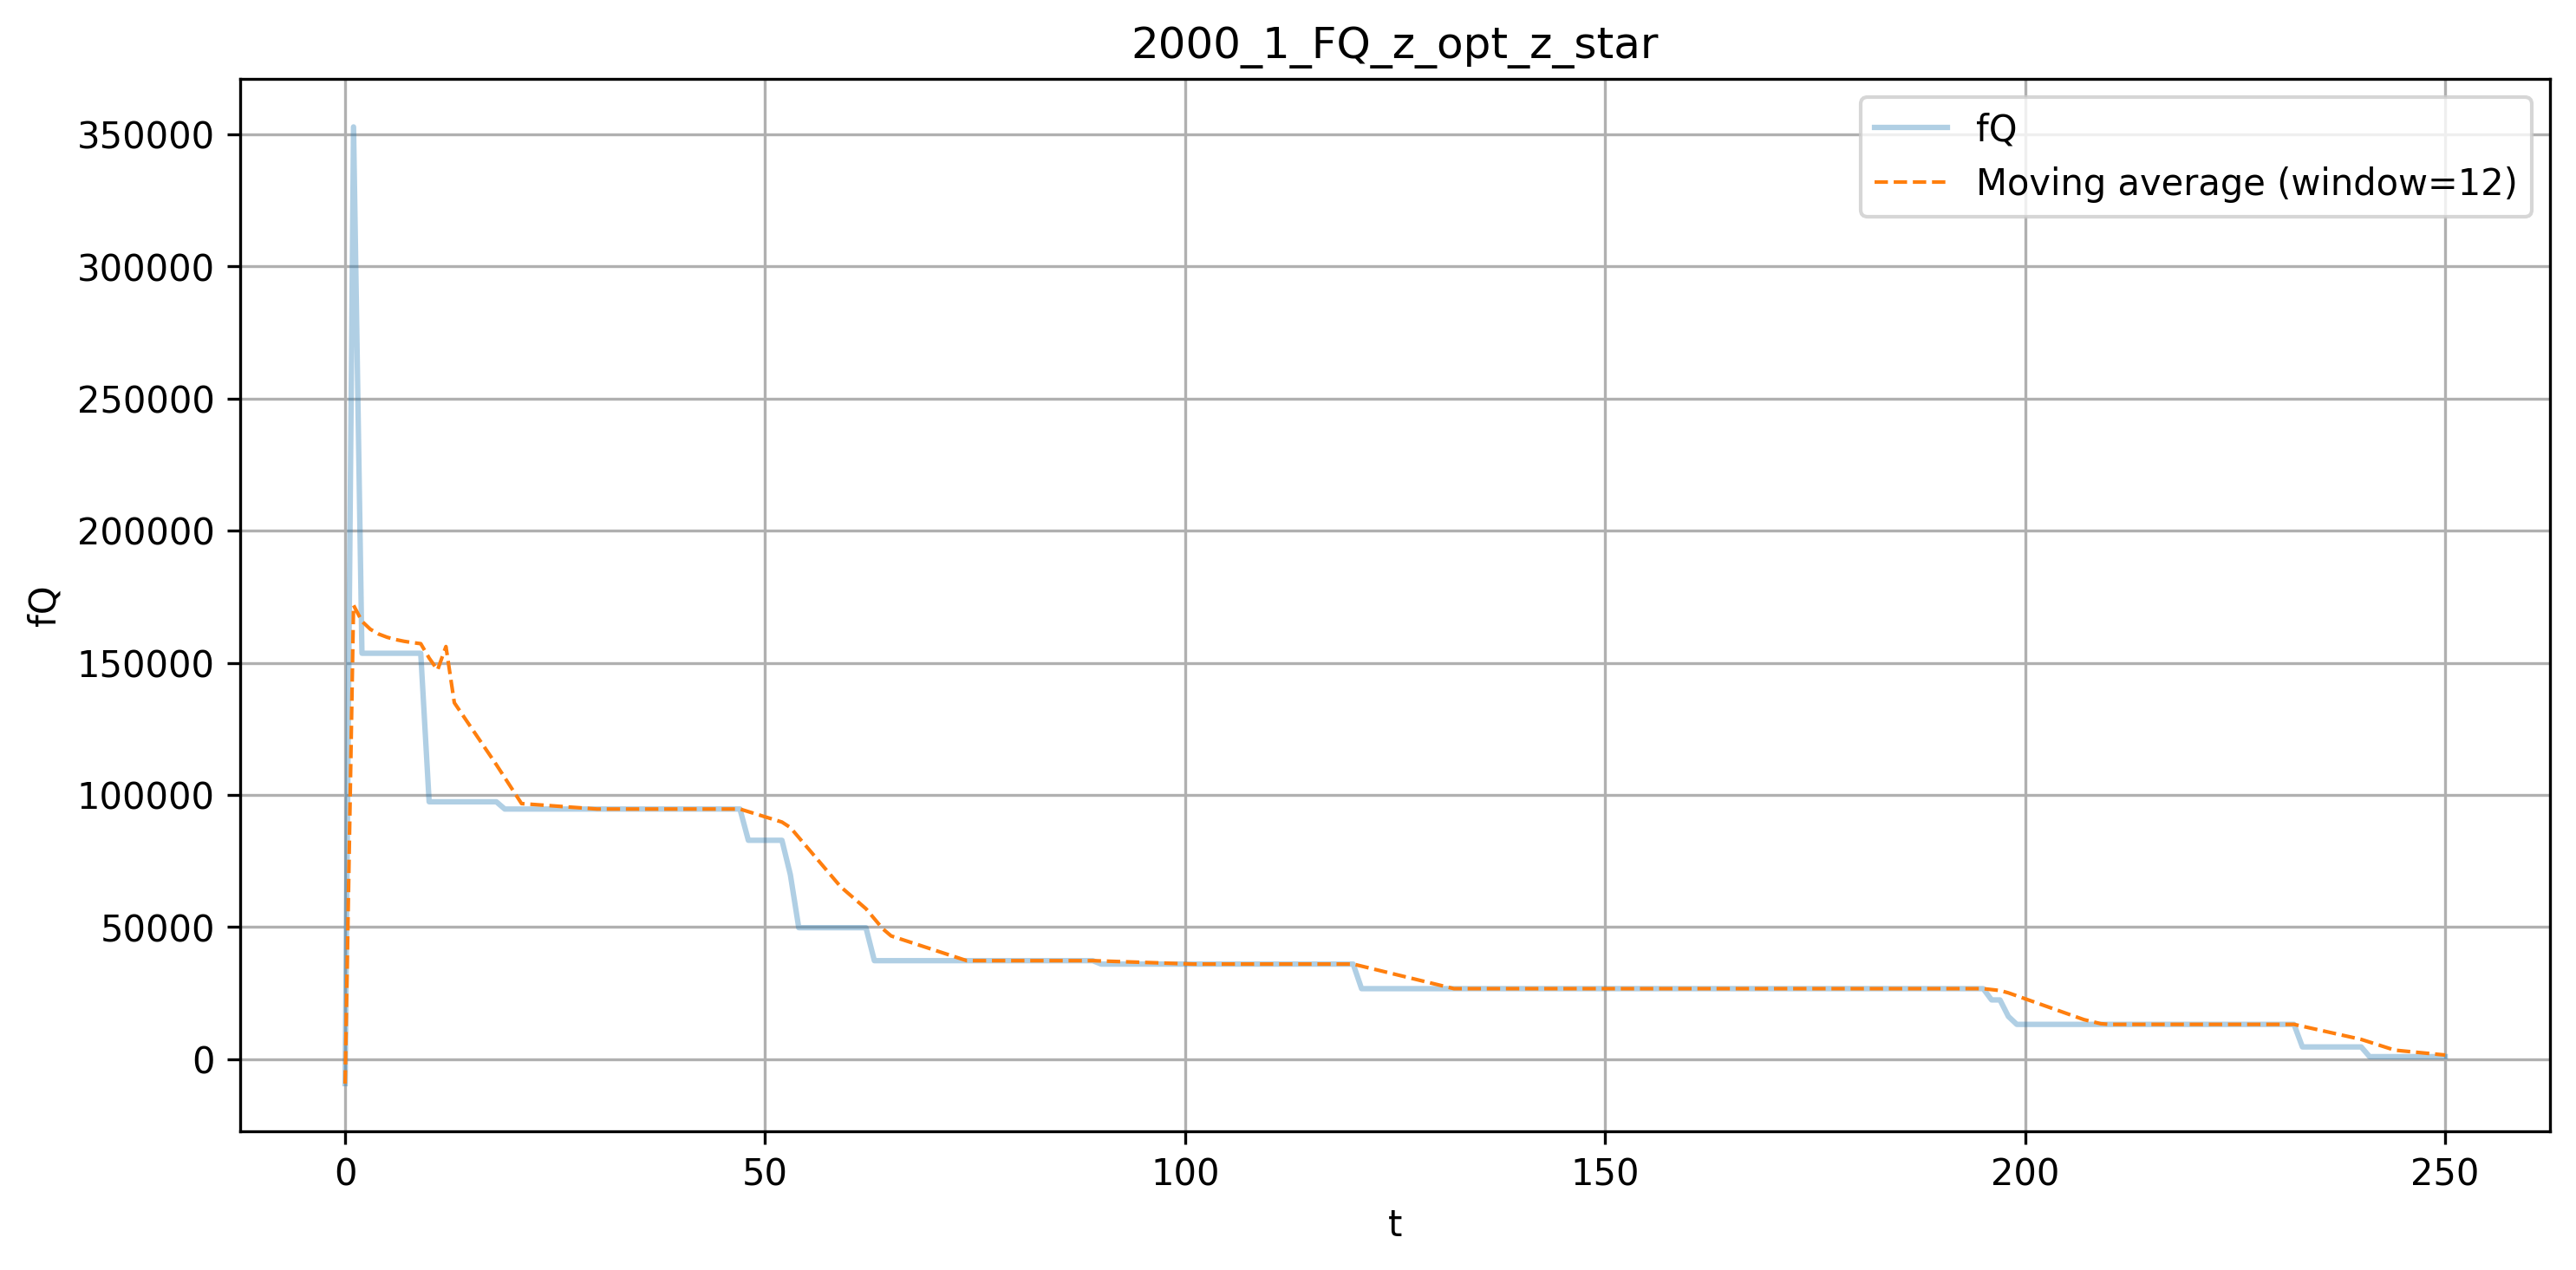
\includegraphics[width=\linewidth]{../Quantum-Annealing-for-solving-QUBO-Problems/test/Lambda_dinamico/ksp_3/lambda_650_dot_C/2000_1_FQ_z_opt_z_star.png}
    \caption{\(f_Q(z_\star)\) con \(\lambda_1\)}
    \label{fig:fQ-zstar-lambda1}
\end{subfigure}
\hfill
\begin{subfigure}{0.495\textwidth}
    \centering
    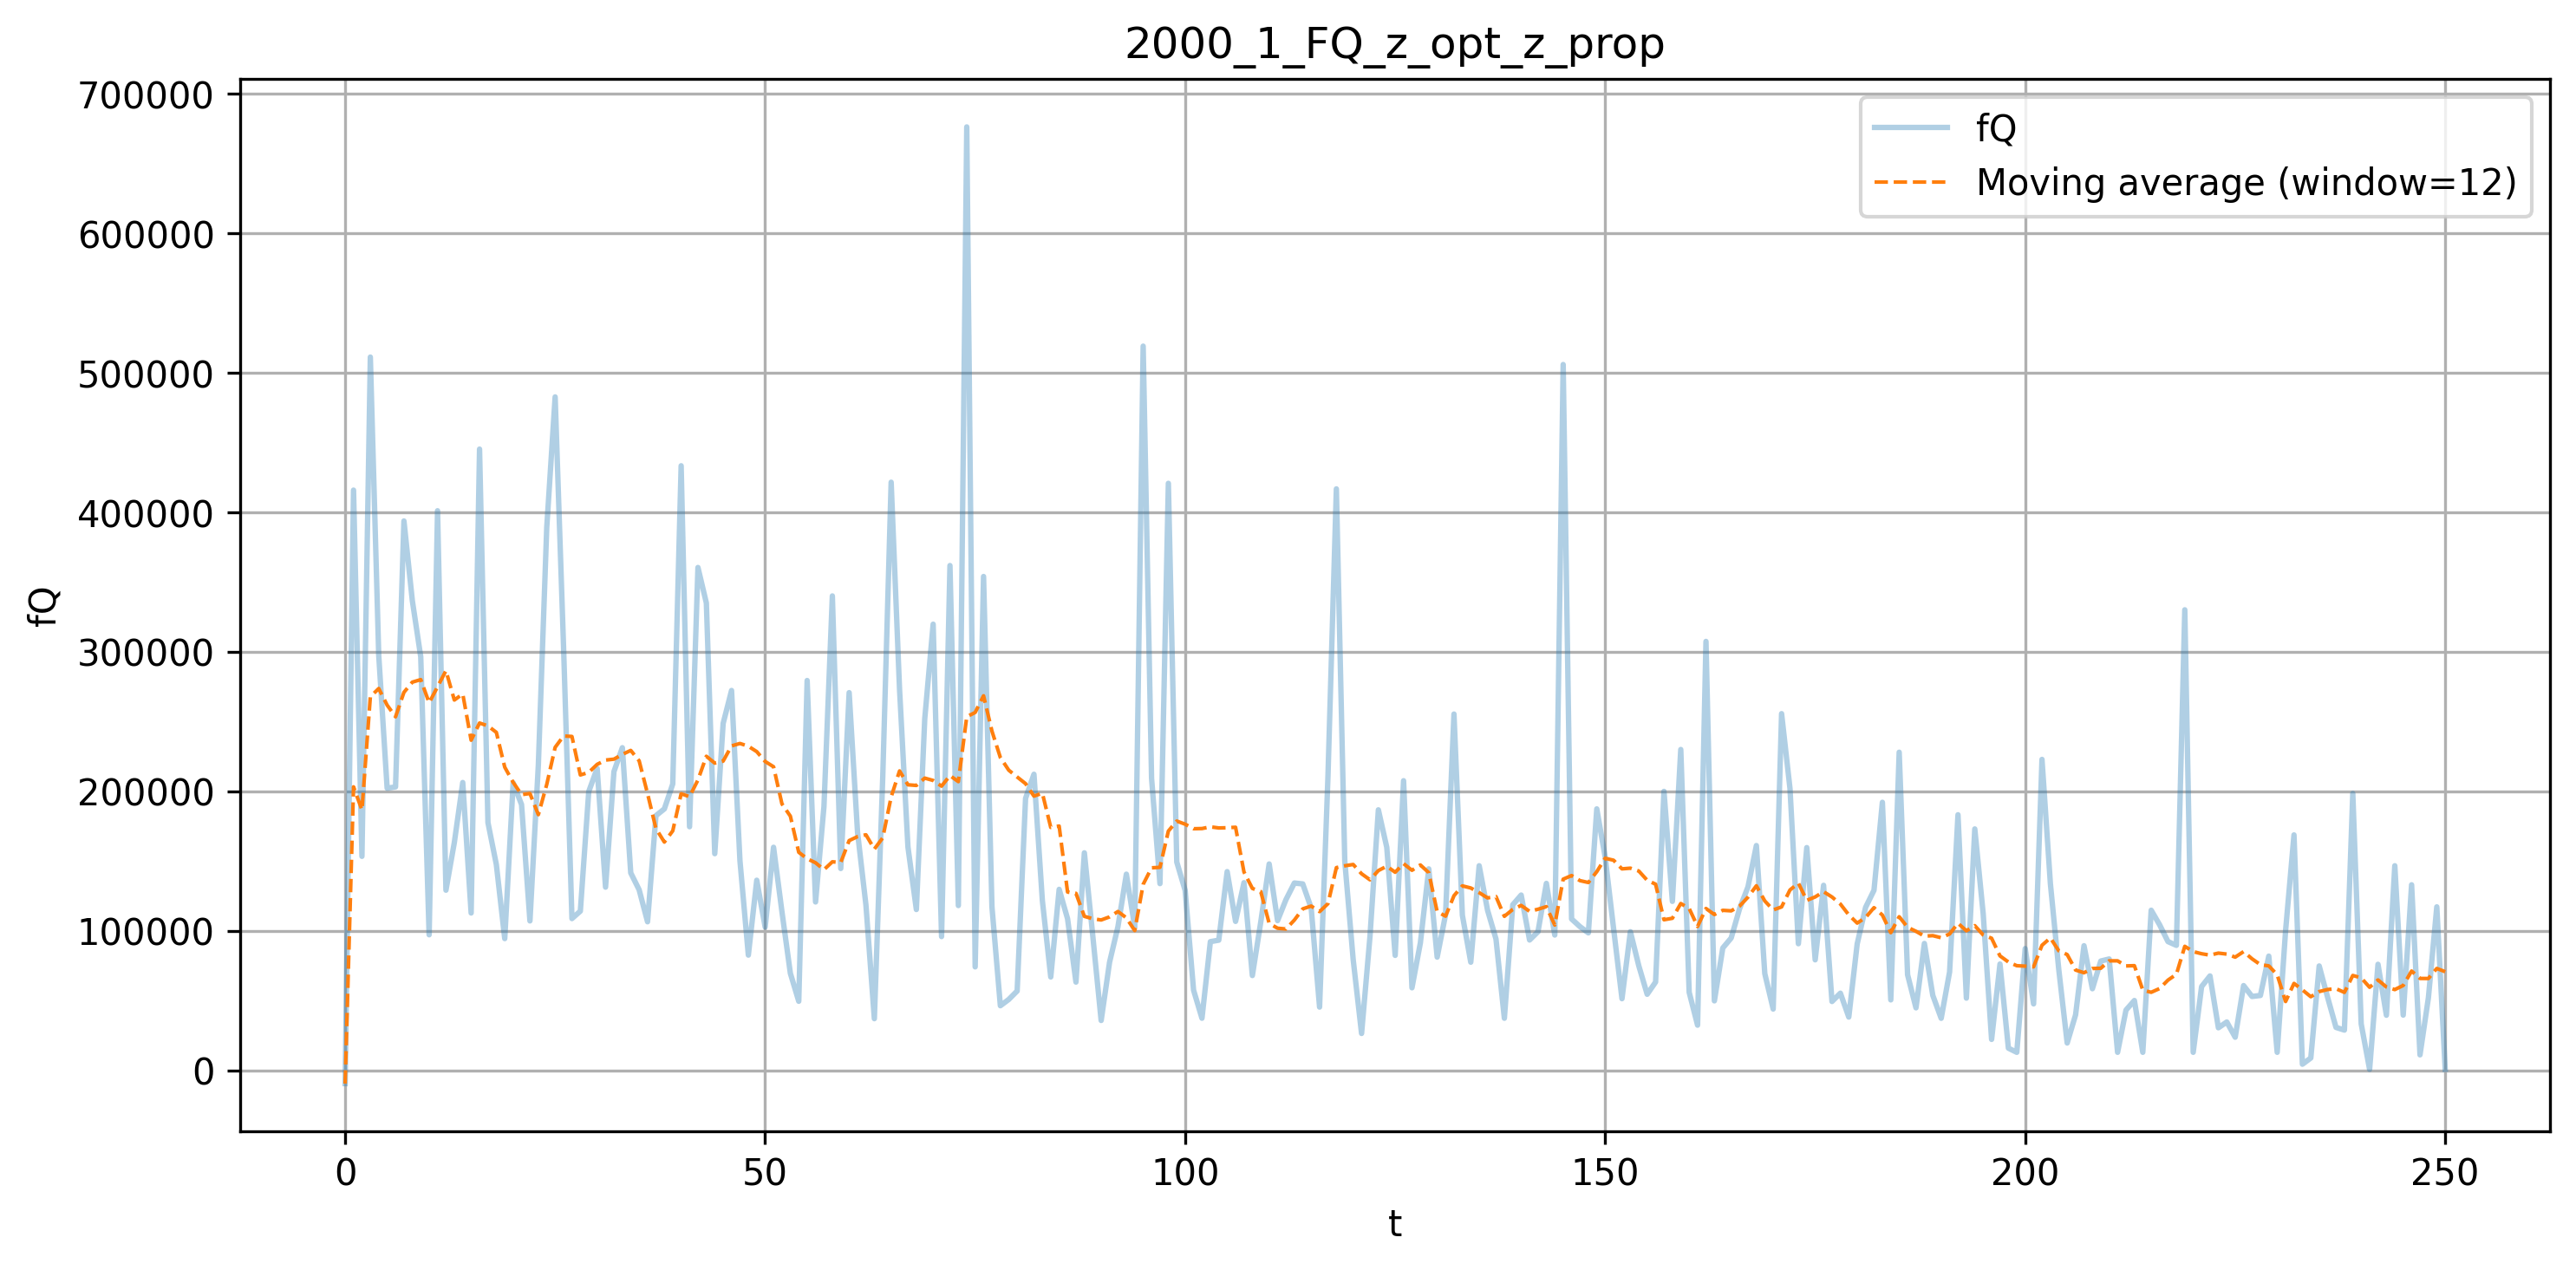
\includegraphics[width=\linewidth]{../Quantum-Annealing-for-solving-QUBO-Problems/test/Lambda_dinamico/ksp_3/lambda_650_dot_C/2000_1_FQ_z_opt_z_prop.png}
    \caption{\(f_Q(z_t)\) con \(\lambda_1\)}
    \label{fig:fQ-zt-lambda1}
\end{subfigure}
\label{fig:confronto-hamming-ksp31}
\end{figure}

\begin{figure}[H]
\centering
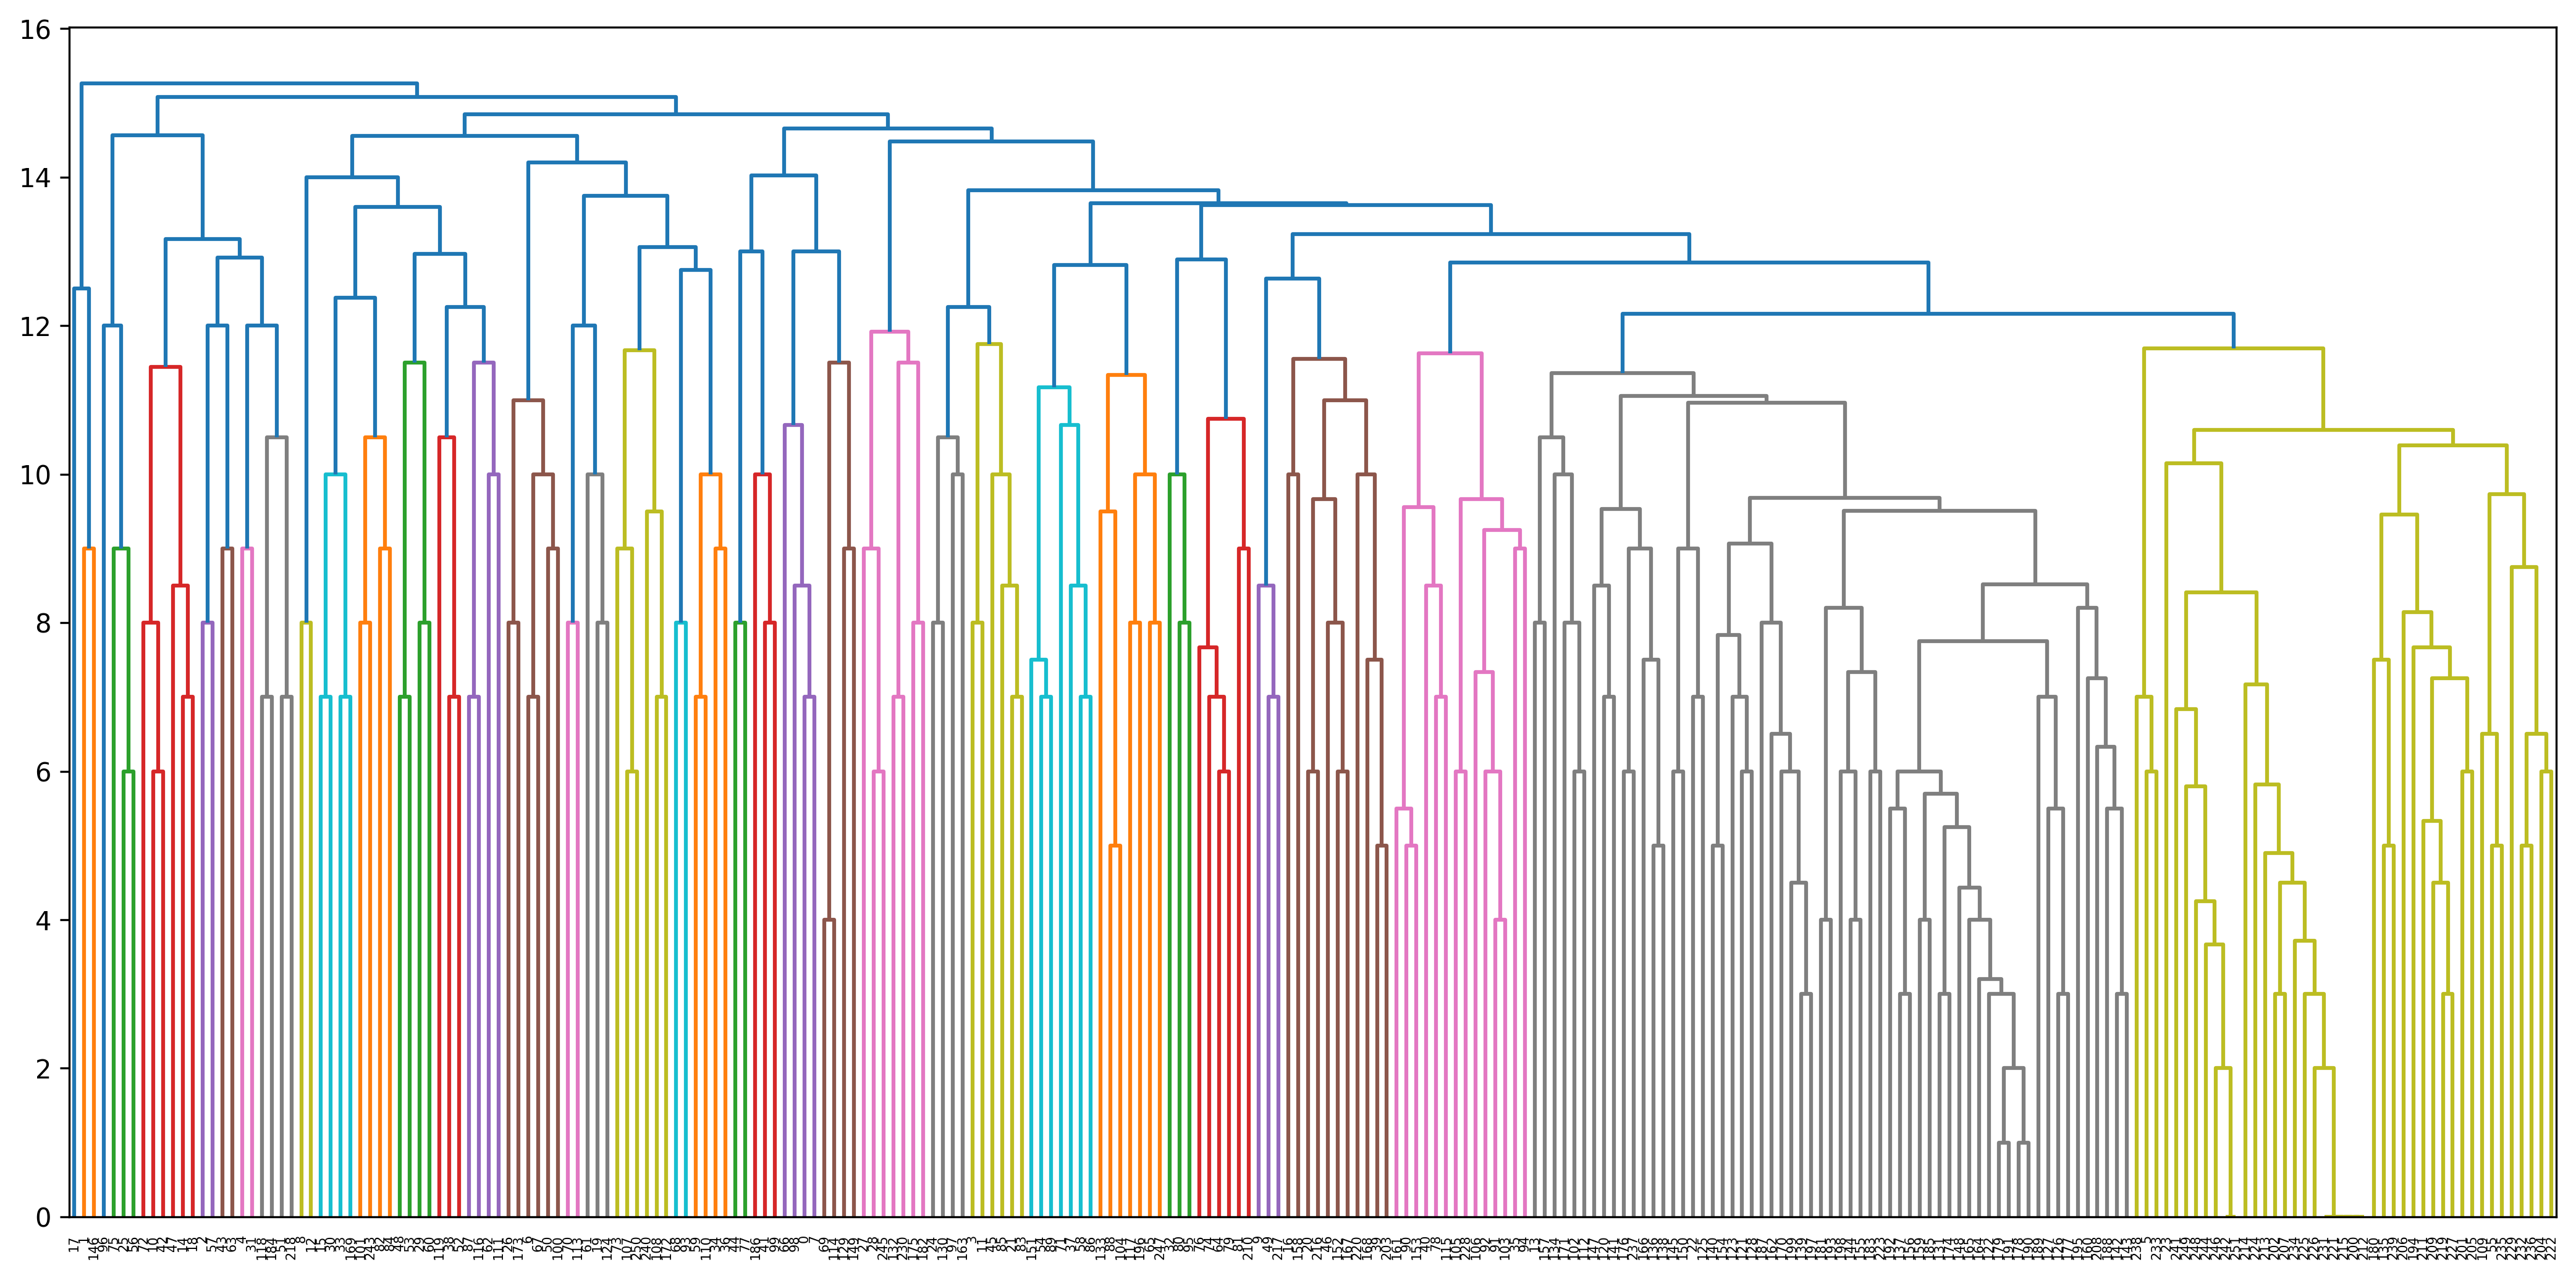
\includegraphics[width=\linewidth]{../Quantum-Annealing-for-solving-QUBO-Problems/test/Lambda_dinamico/ksp_3/lambda_650_dot_C/dendrogram_2000_1.png}
\caption{Agglomerative Clustering Dendogram}
\label{fig:AgglomerativeClustering-ksp3}
\end{figure}

\clearpage
\begin{figure}[H]
\centering
\begin{subfigure}{0.495\textwidth}
    \centering
    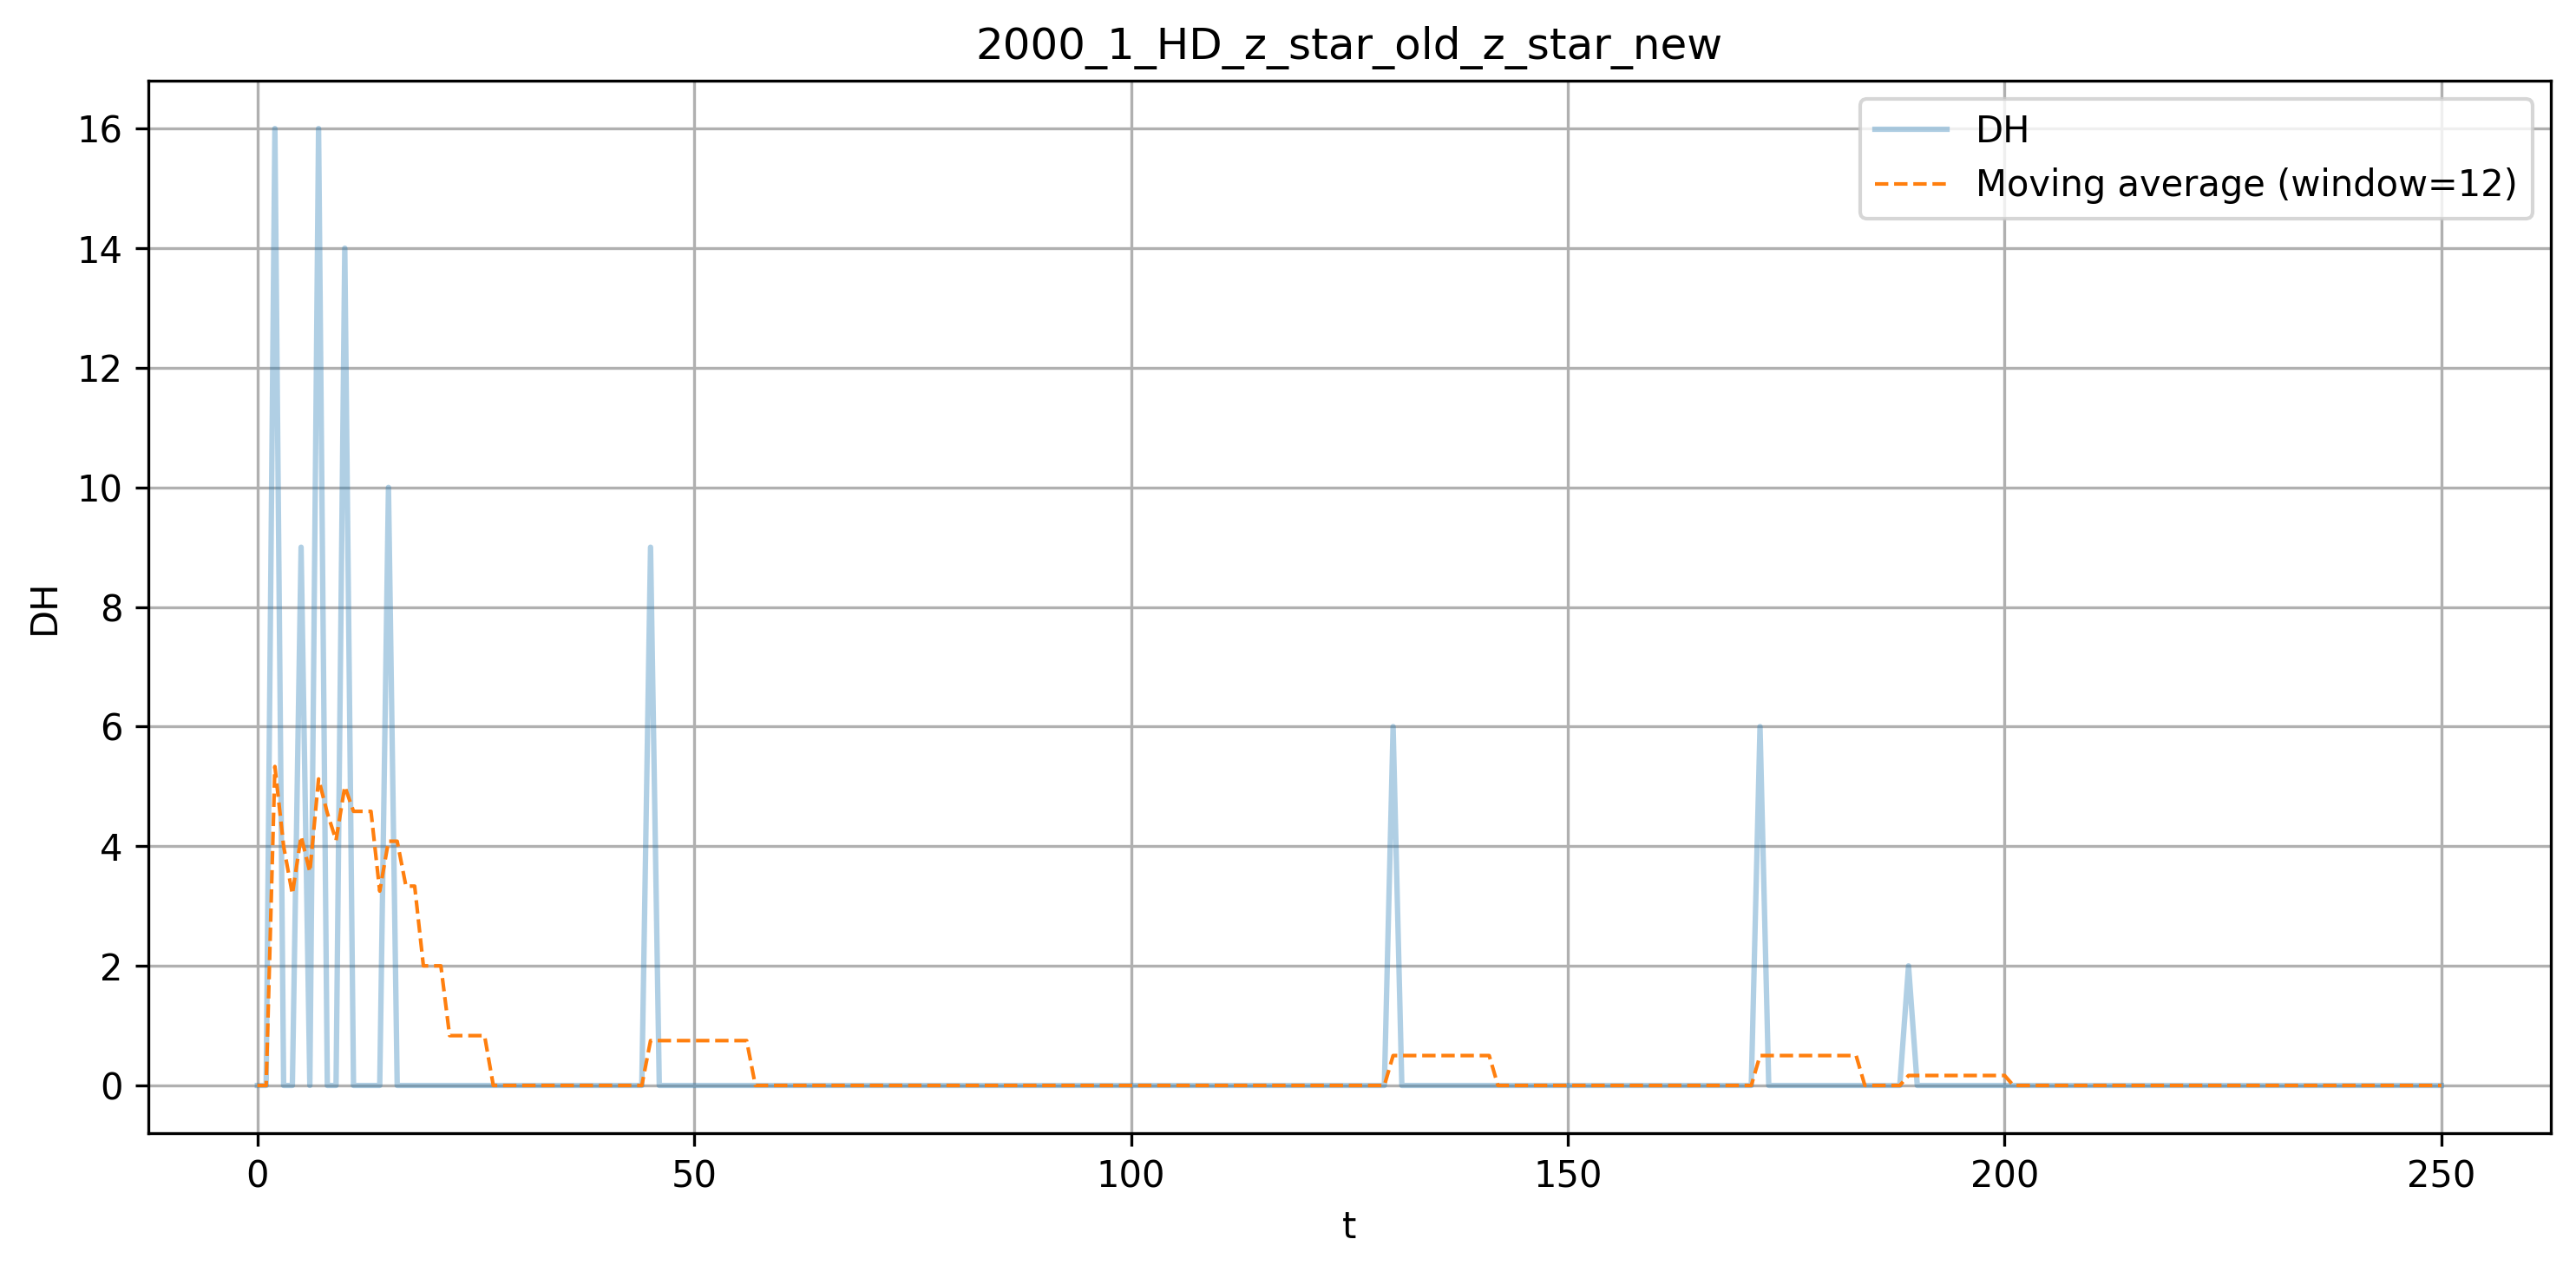
\includegraphics[width=\linewidth]{../Quantum-Annealing-for-solving-QUBO-Problems/test/Lambda_dinamico/ksp_3/lambda_div_3/2000_1_HD_z_star_old_z_star_new.png}
    \caption{\(d_H(z_\star^{old}, z_\star^{new})\) con \(\lambda_2\)}
    \label{fig:hd-zstarold-zstarnew-lambda2}
\end{subfigure}
\hfill
\begin{subfigure}{0.495\textwidth}
    \centering
    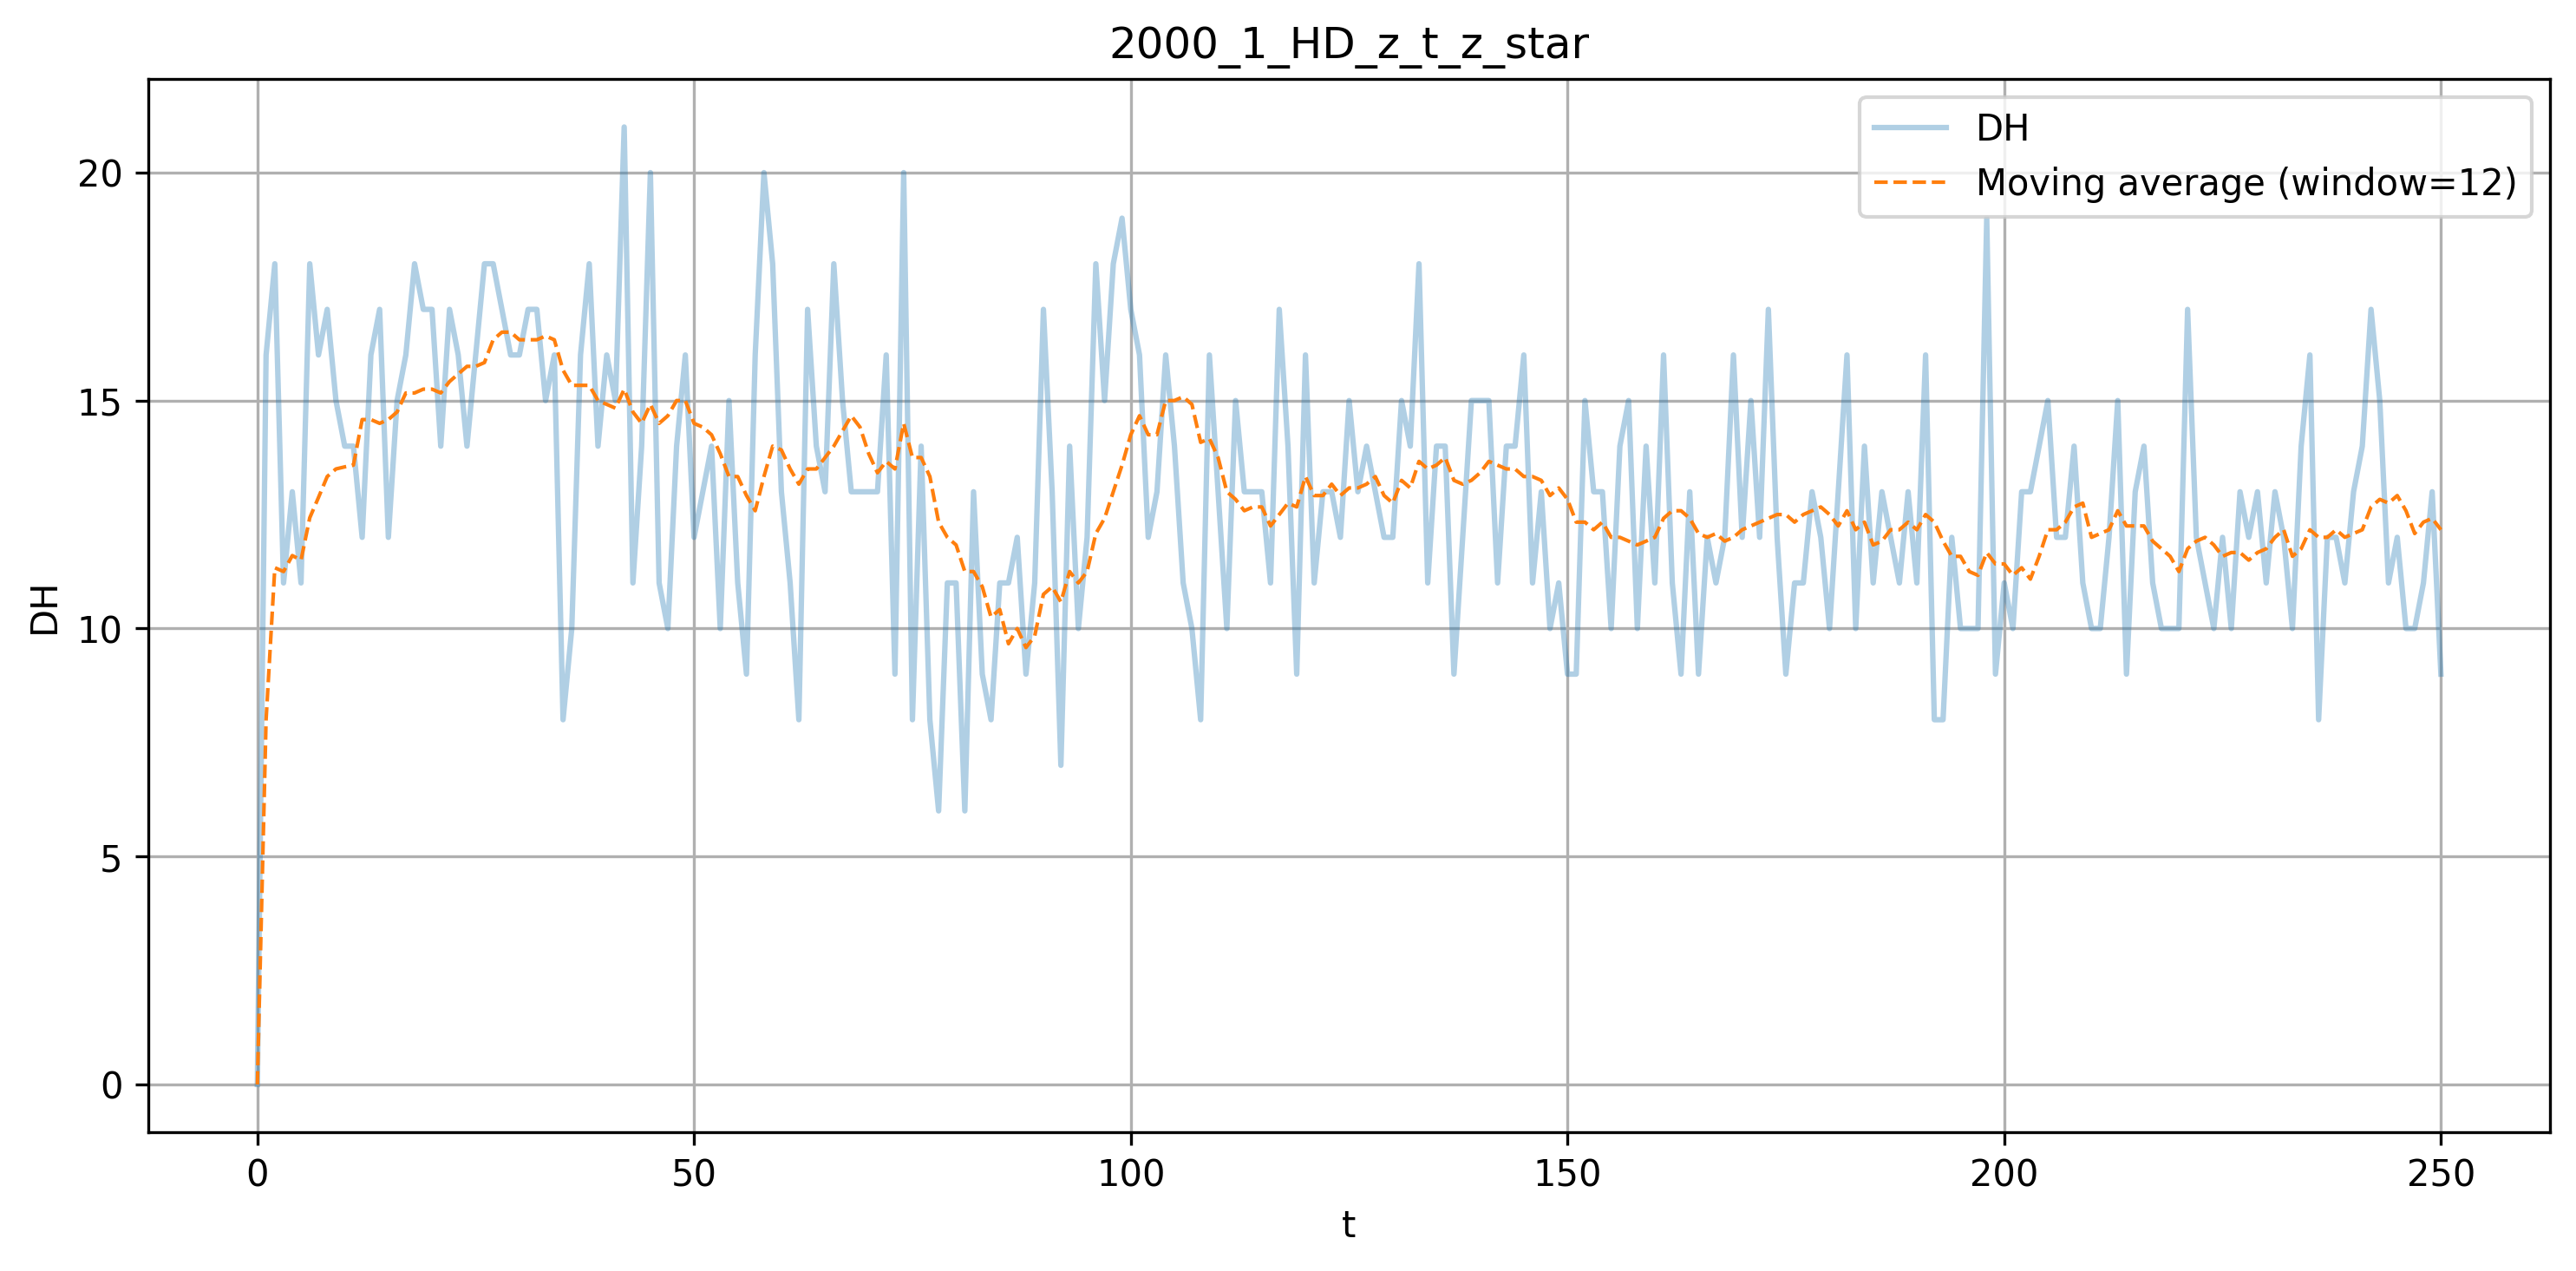
\includegraphics[width=\linewidth]{../Quantum-Annealing-for-solving-QUBO-Problems/test/Lambda_dinamico/ksp_3/lambda_div_3/2000_1_HD_z_t_z_star.png}
    \caption{\(d_H(z_t, z_\star)\) con \(\lambda_2\)}
    \label{fig:hd-zt-zstar-lambda2}
\end{subfigure}

\vspace{0.35cm}

\begin{subfigure}{0.495\textwidth}
    \centering
    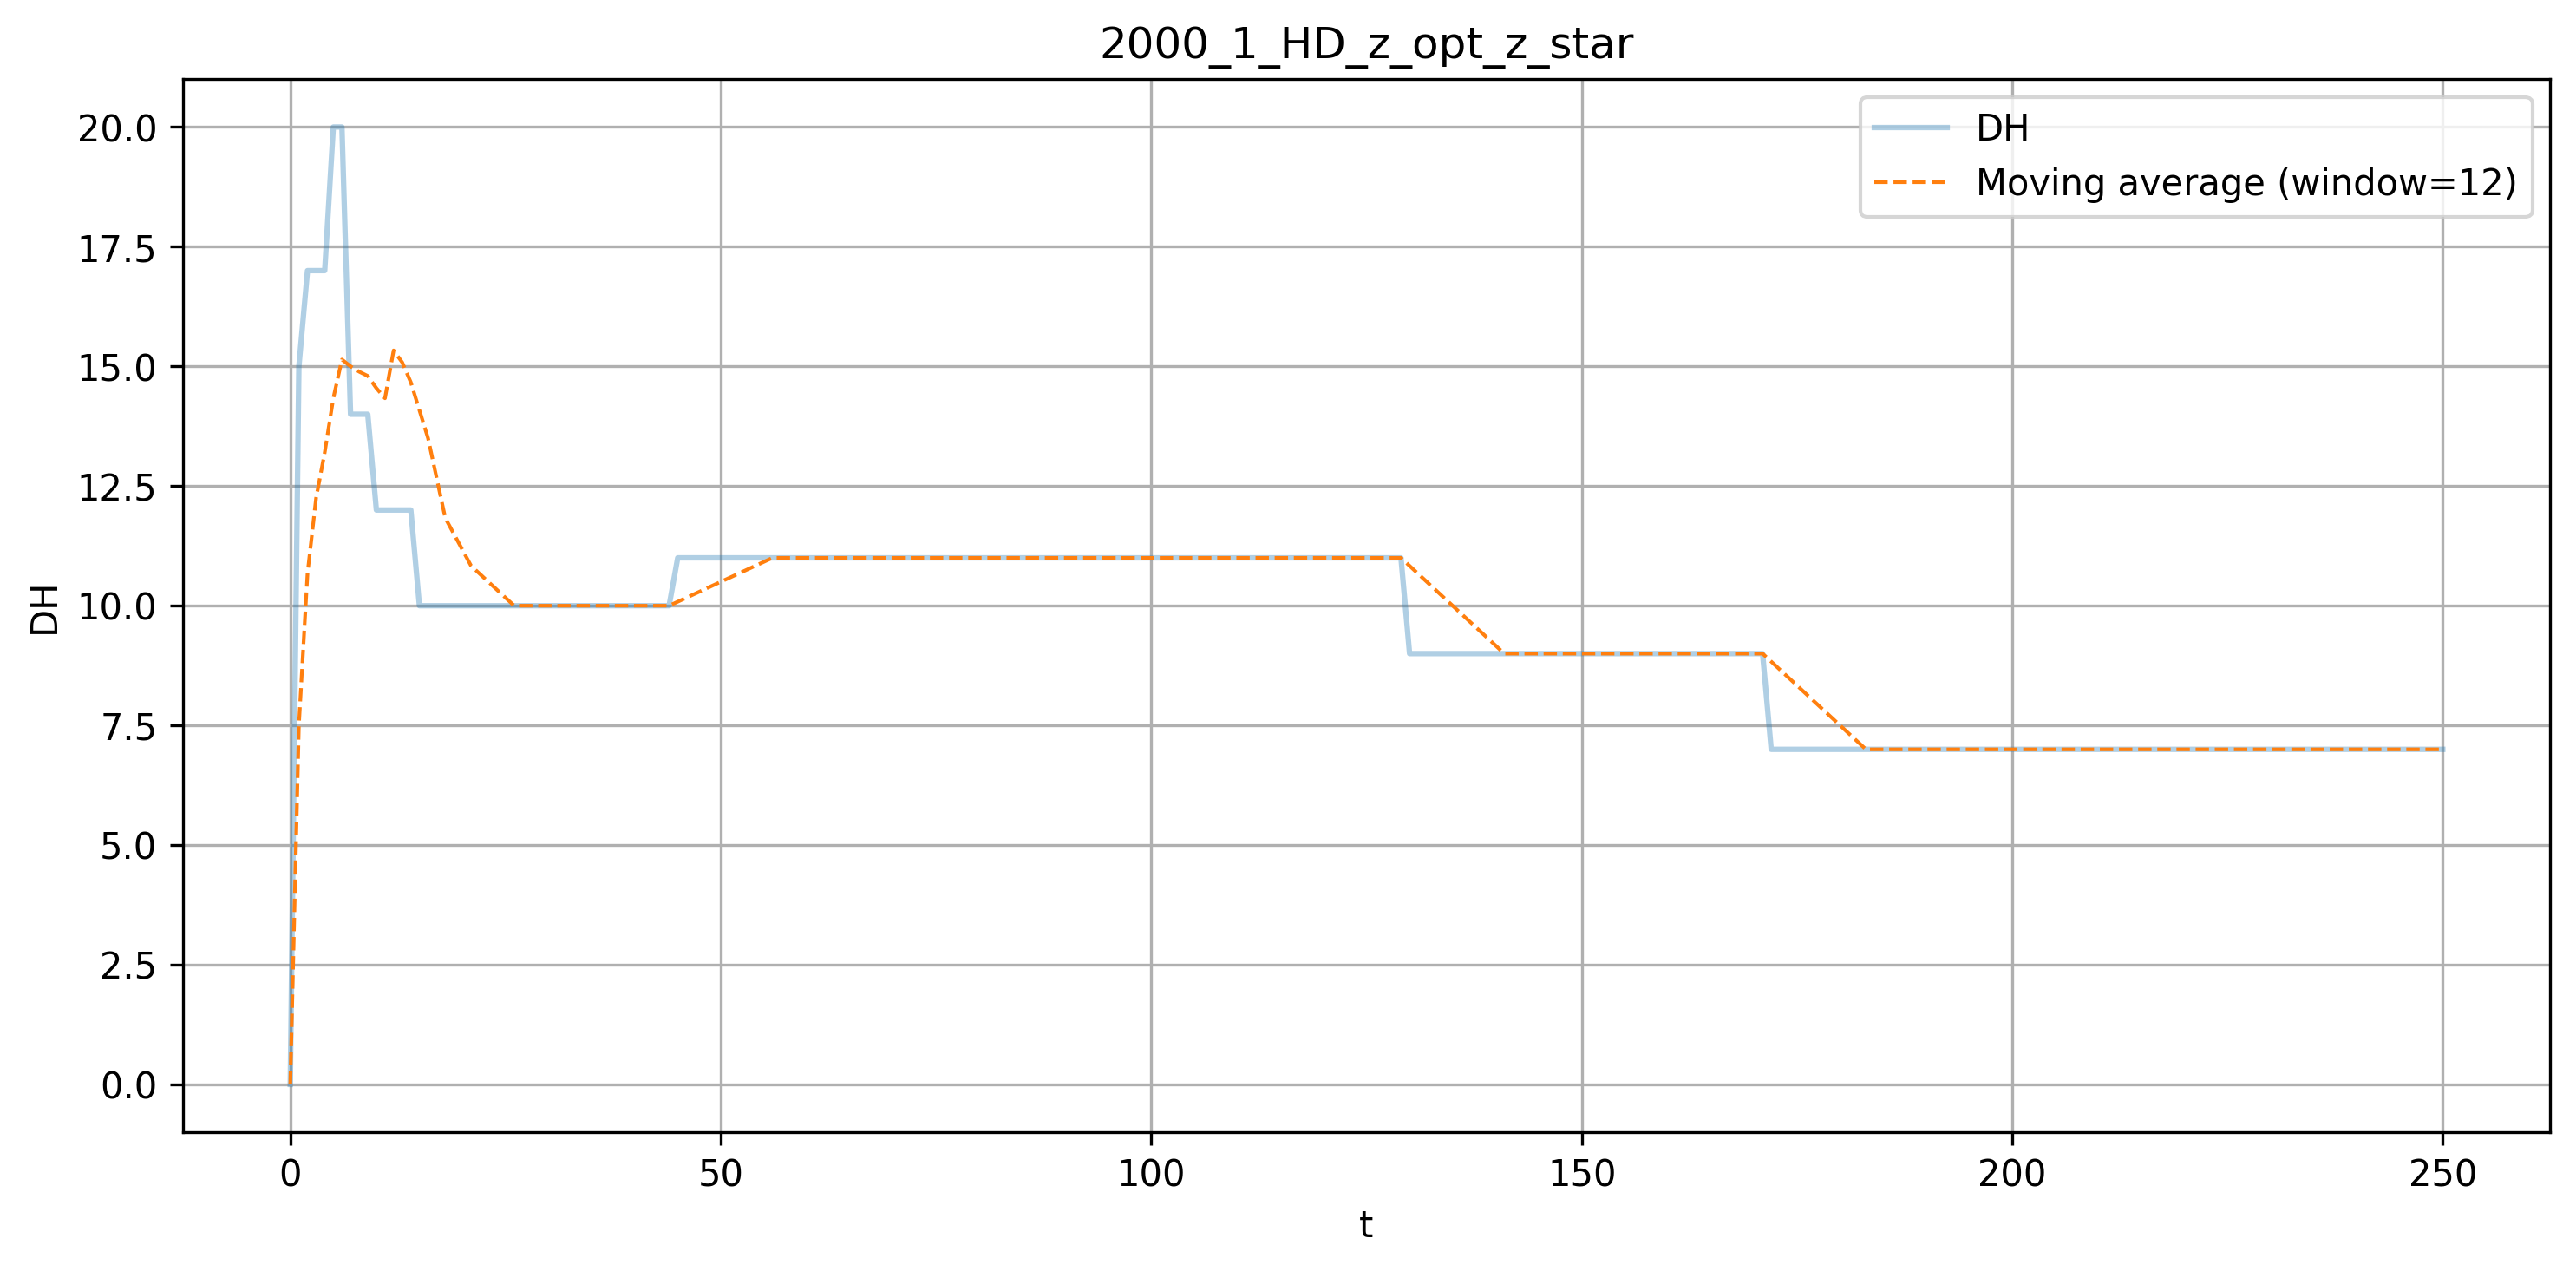
\includegraphics[width=\linewidth]{../Quantum-Annealing-for-solving-QUBO-Problems/test/Lambda_dinamico/ksp_3/lambda_div_3/2000_1_HD_z_opt_z_star.png}
    \caption{\(d_H(z_{opt}, z_\star)\) con \(\lambda_2\)}
    \label{fig:hd-zopt-zstar-lambda2}
\end{subfigure}
\hfill
\begin{subfigure}{0.495\textwidth}
    \centering
    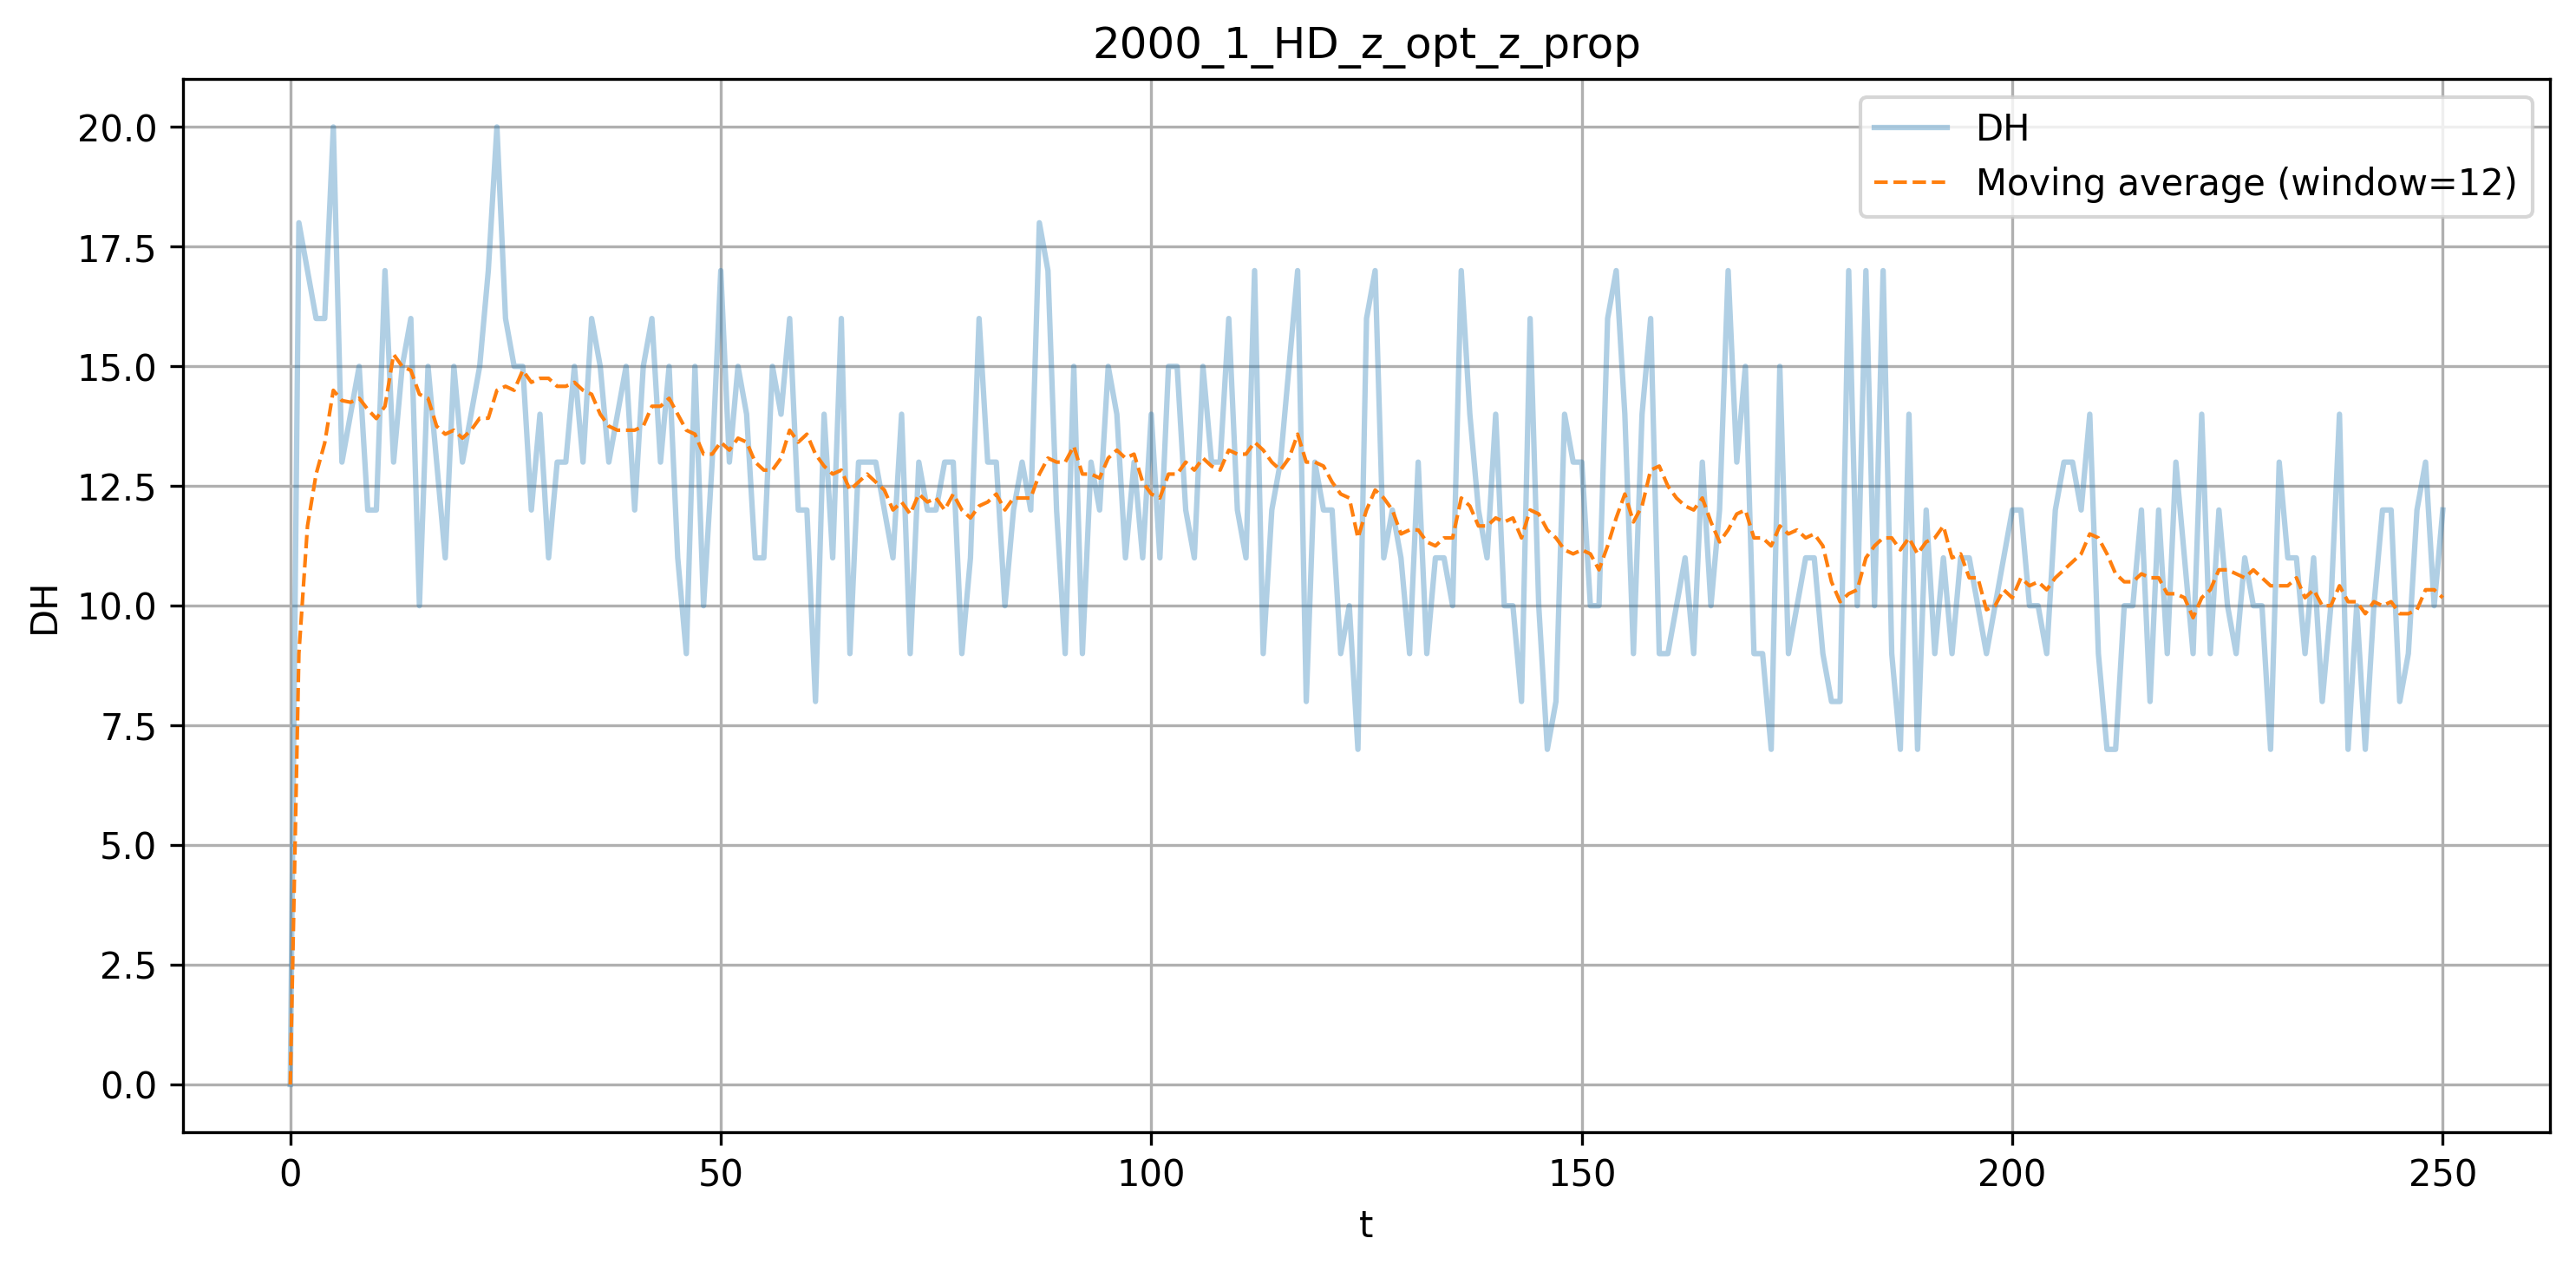
\includegraphics[width=\linewidth]{../Quantum-Annealing-for-solving-QUBO-Problems/test/Lambda_dinamico/ksp_3/lambda_div_3/2000_1_HD_z_opt_z_prop.png}
    \caption{\(d_H(z_{opt}, z_t)\) con \(\lambda_2\)}
    \label{fig:hd-zopt-zt-lambda2}
\end{subfigure}

\vspace{0.35cm}

\begin{subfigure}{0.495\textwidth}
    \centering
    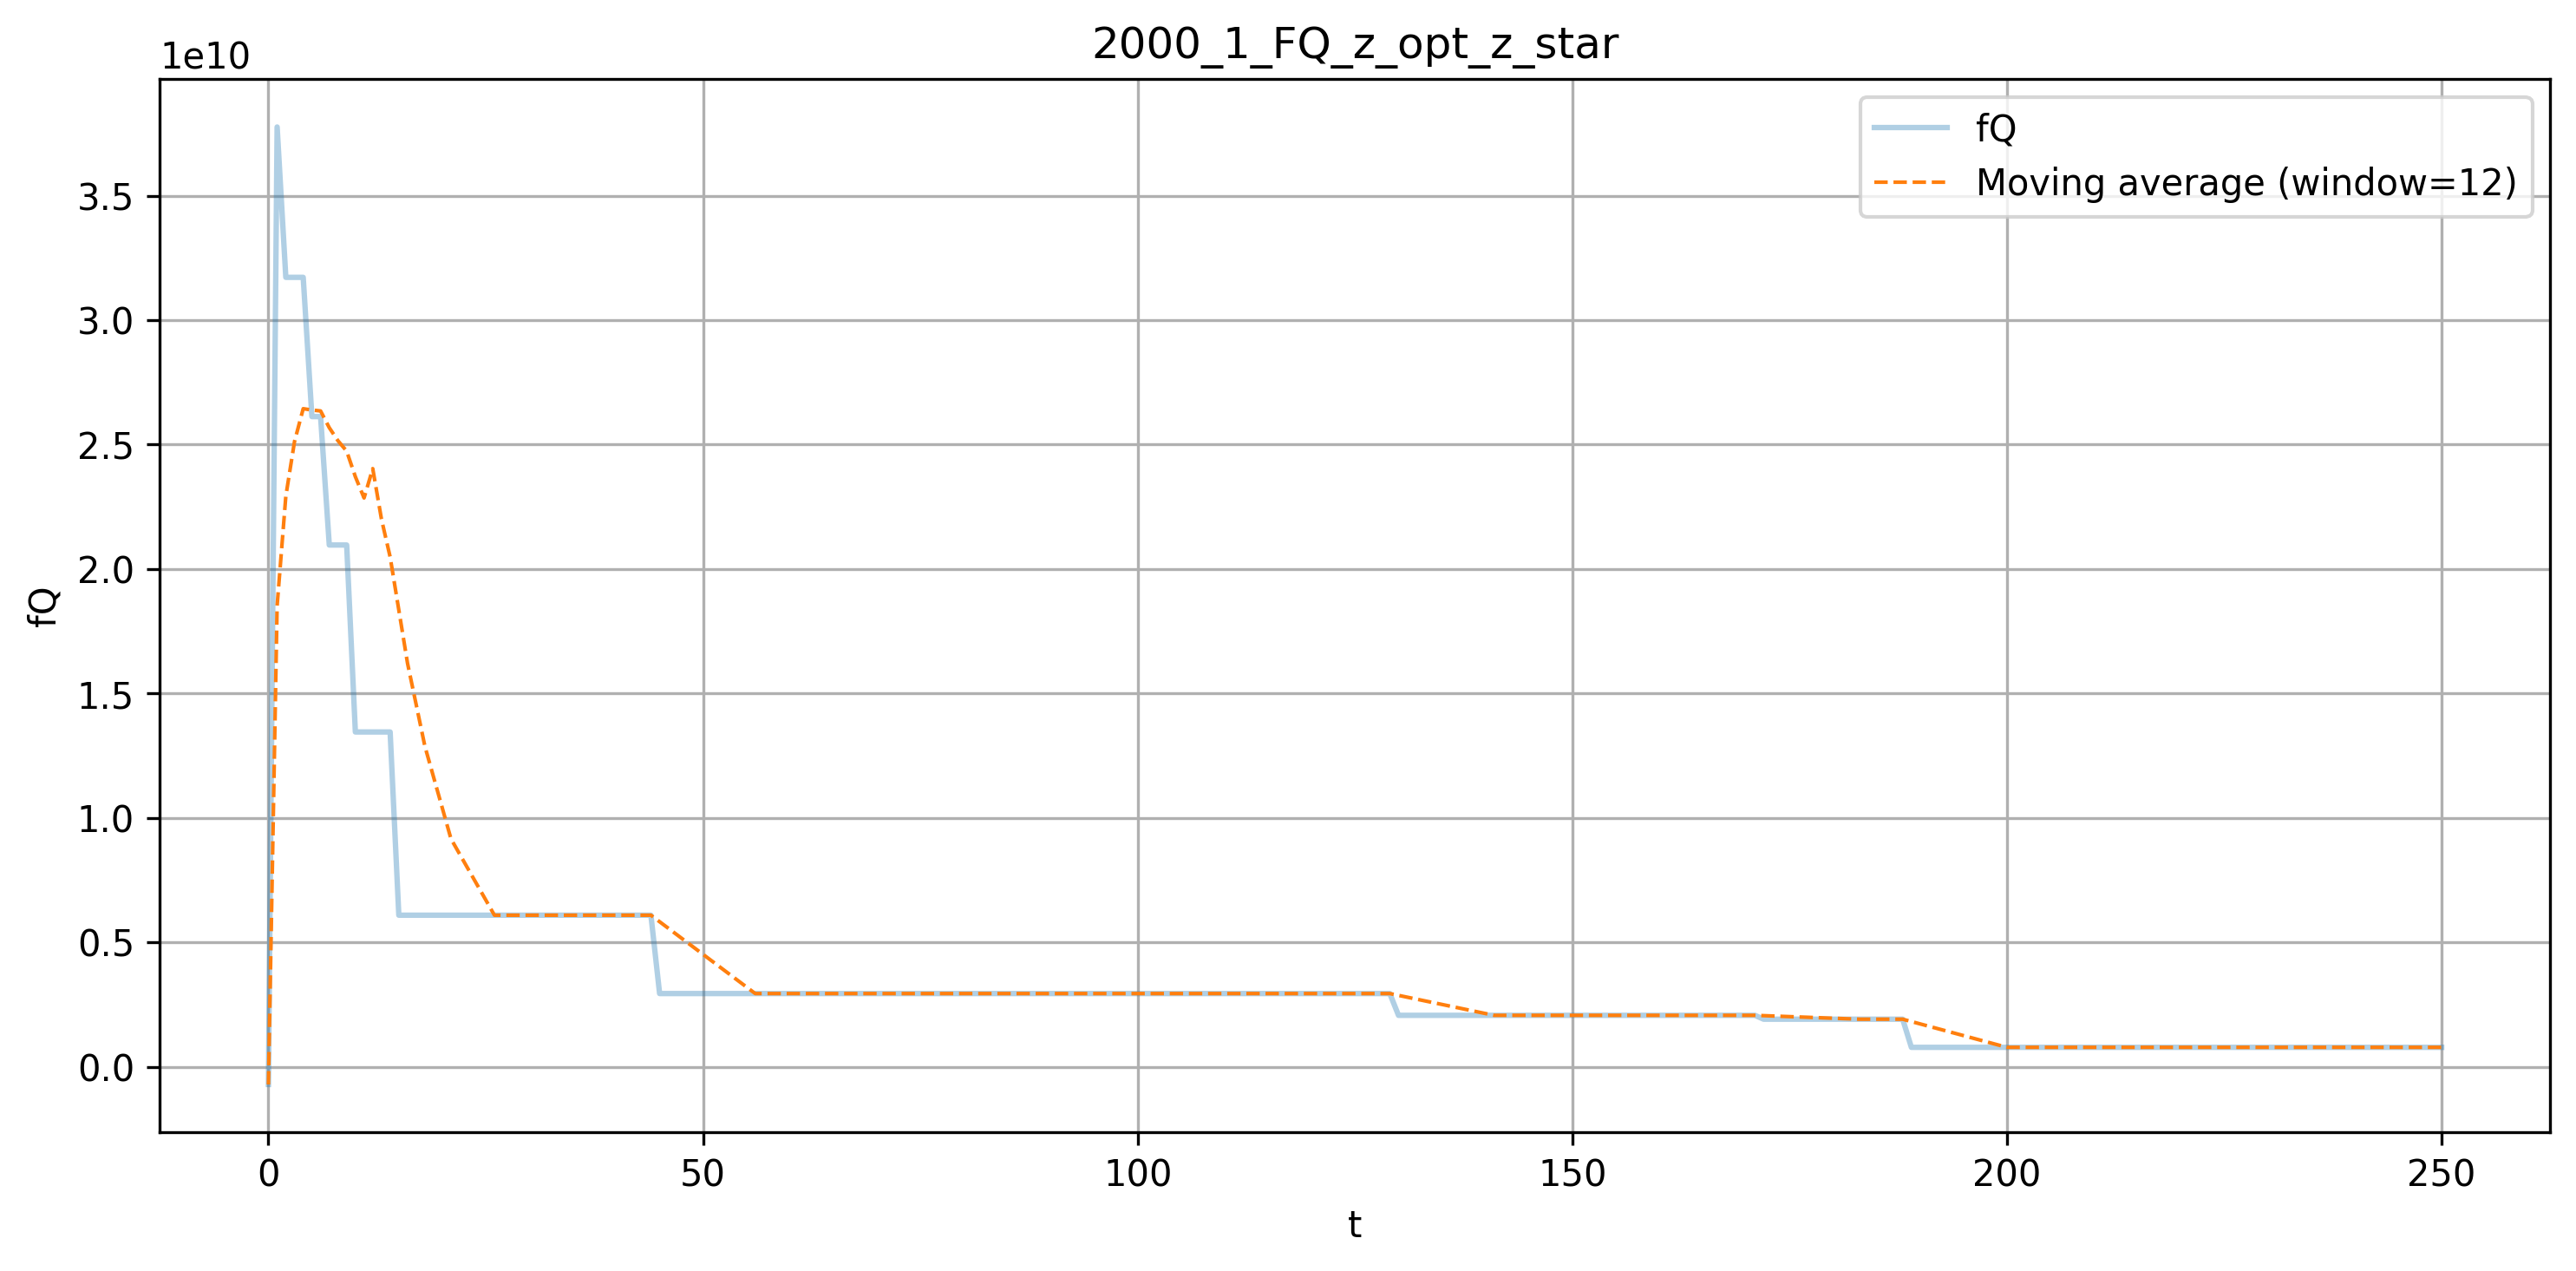
\includegraphics[width=\linewidth]{../Quantum-Annealing-for-solving-QUBO-Problems/test/Lambda_dinamico/ksp_3/lambda_div_3/2000_1_FQ_z_opt_z_star.png}
    \caption{\(f_Q(z_\star)\) con \(\lambda_2\)}
    \label{fig:fQ-zstar-lambda2}
\end{subfigure}
\hfill
\begin{subfigure}{0.495\textwidth}
    \centering
    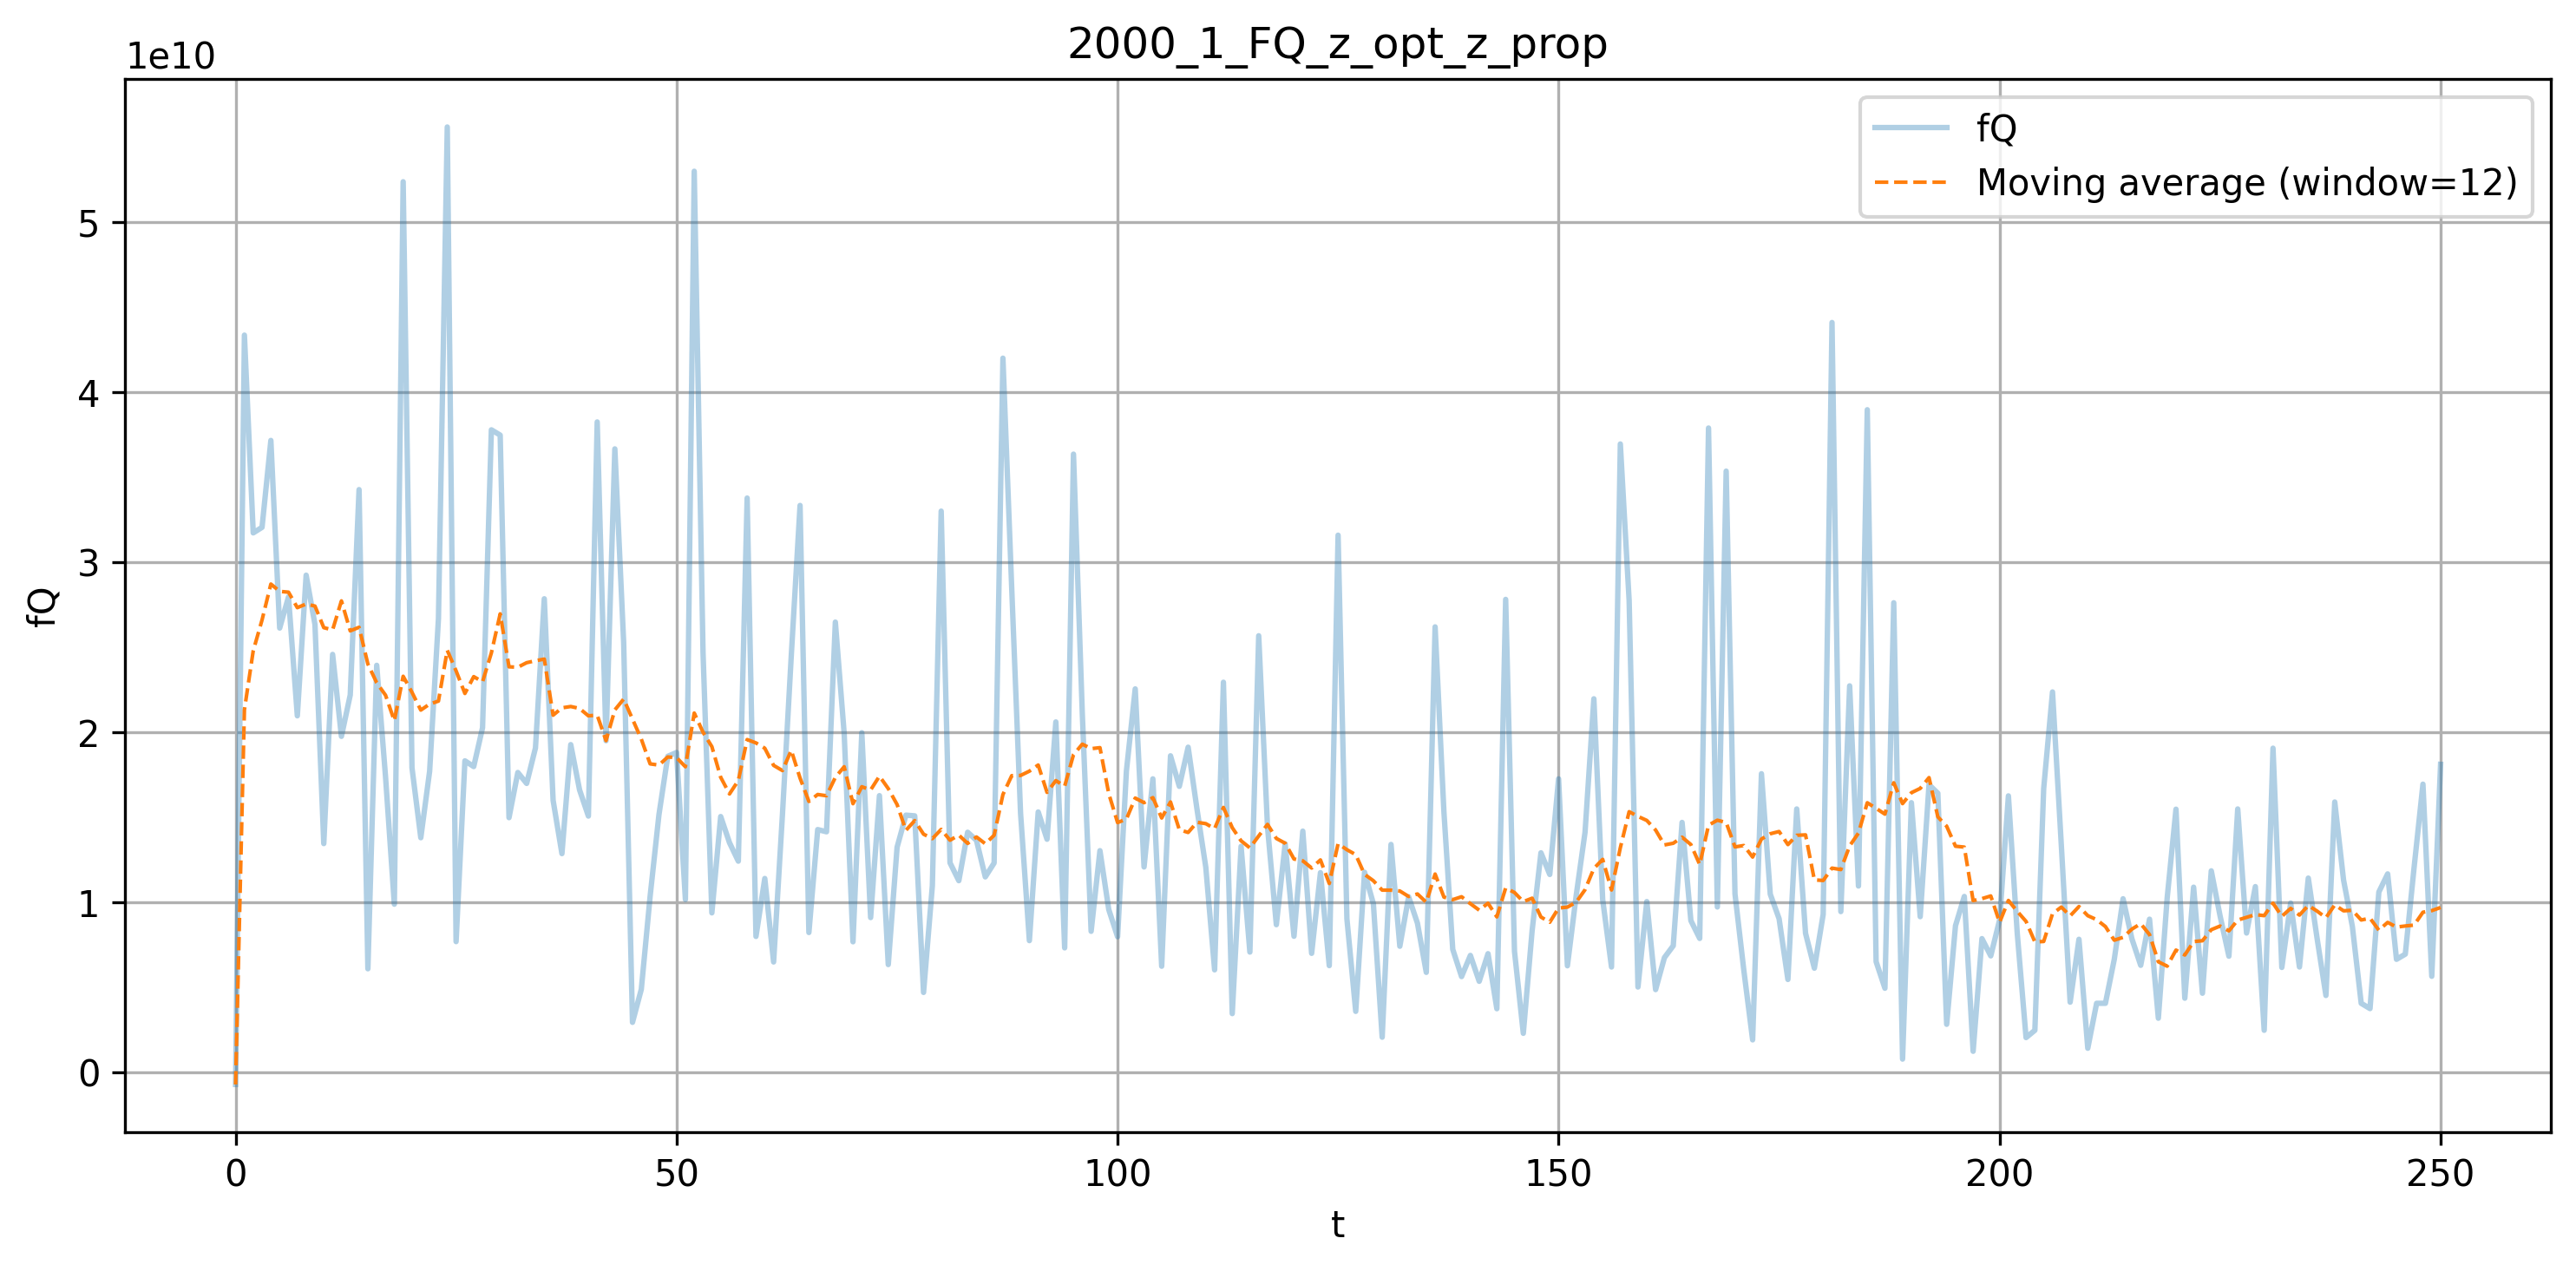
\includegraphics[width=\linewidth]{../Quantum-Annealing-for-solving-QUBO-Problems/test/Lambda_dinamico/ksp_3/lambda_div_3/2000_1_FQ_z_opt_z_prop.png}
    \caption{\(f_Q(z_t)\) con \(\lambda_2\)}
    \label{fig:fQ-zt-lambda2}
\end{subfigure}
\label{fig:confronto-hamming-ksp32}
\end{figure}

\begin{figure}[H]
\centering
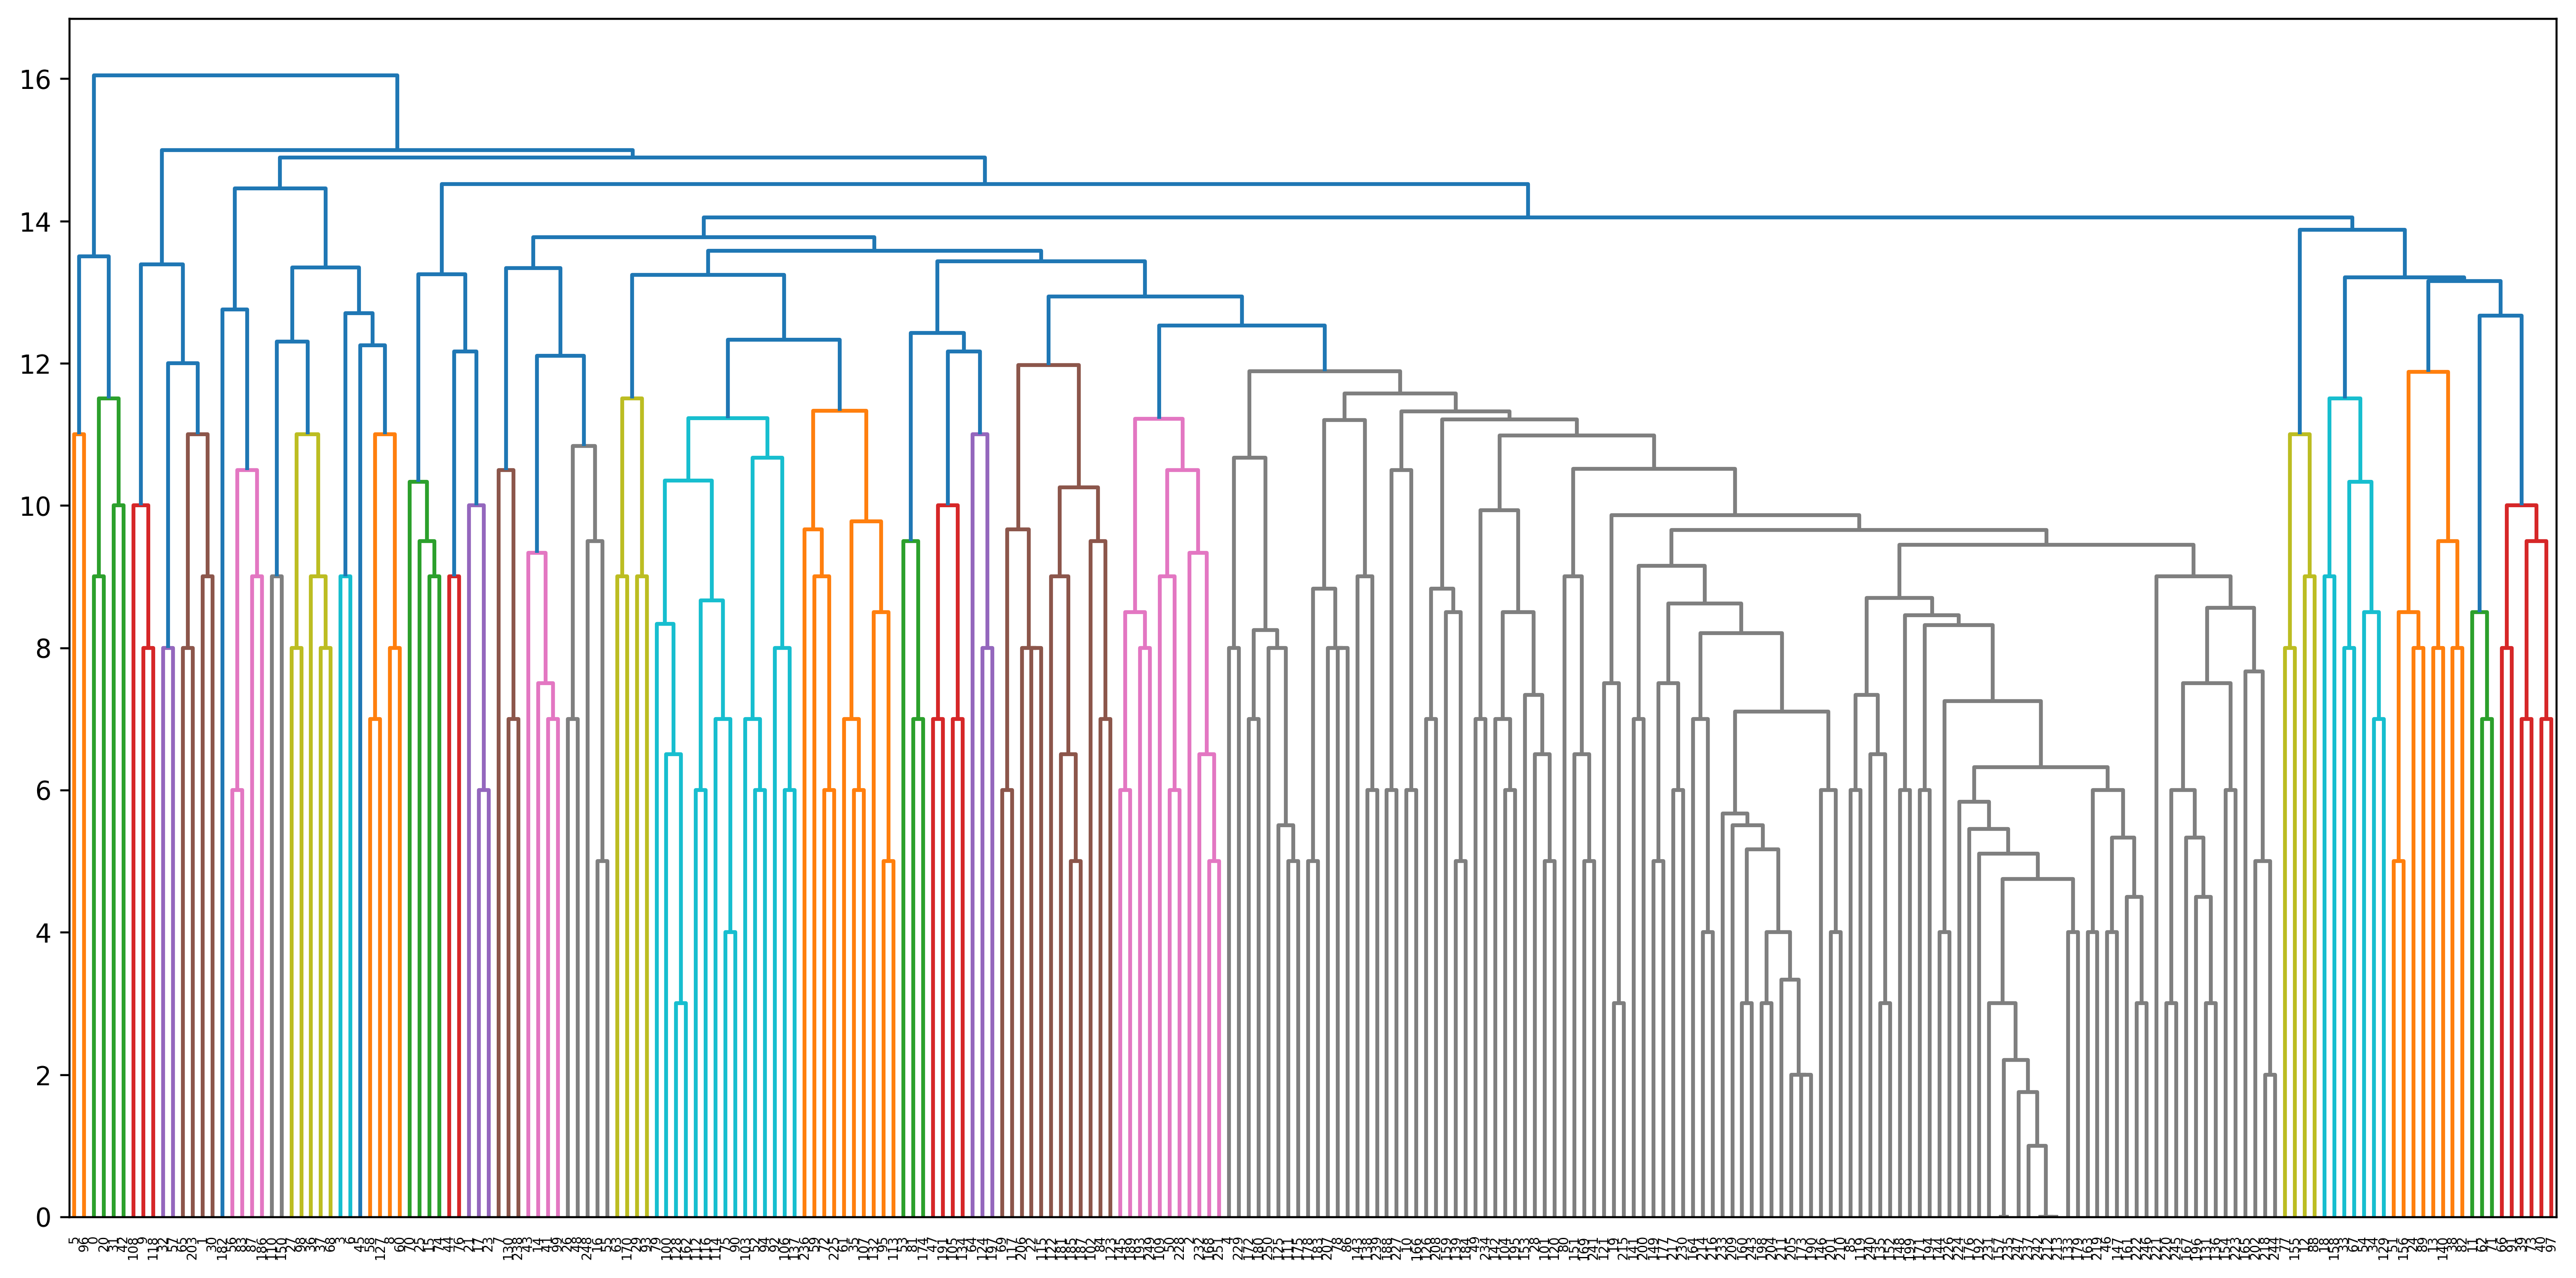
\includegraphics[width=\linewidth]{../Quantum-Annealing-for-solving-QUBO-Problems/test/Lambda_dinamico/ksp_3/lambda_div_3/dendrogram_2000_1.png}
\caption{Agglomerative Clustering Dendogram}
\label{fig:AgglomerativeClustering-ksp3}
\end{figure}

\clearpage
\subsection{ksp\_2}

\begin{table}[h]
\centering
\begin{tabular}{lcc}
\hline
\textbf{Metrica} & \(\lambda_1\) & \(\lambda_2\) \\
\hline
Numero cluster & 45 & 50 \\
Dimensione cluster massimo & 108 & 86 \\
Cluster z best & [1, 108] & [8, 86] \\
Single clusters & 7 & 3 \\
\(f_Q\) medoid & 594217.38 & 494496241717.67 \\
Profit medoid & 10760 & 11909 \\
Weight medoid & 4728 & 8042 \\
\hline
\(f_Q\) Min Found QALS & 546064.29 & 218237506978.67 \\
Profit Found QALS & 11186 & 8984 \\
Weight Found QALS & 4589 & 5738 \\
\hline
\(f_Q\) Min Found NO QALS & -54748.31 & -10200709849.33 \\
Profit Found NO QALS & 7740 & 5669 \\
Weight Found NO QALS & 978 & 1001 \\
\hline
\end{tabular}

\caption{Confronto dei risultati ottenuti con QALS e senza QALS.}
\label{tab:confronto-qals-noqals}
\end{table}

\begin{figure}[H]
\centering
\begin{subfigure}{0.495\textwidth}
    \centering
    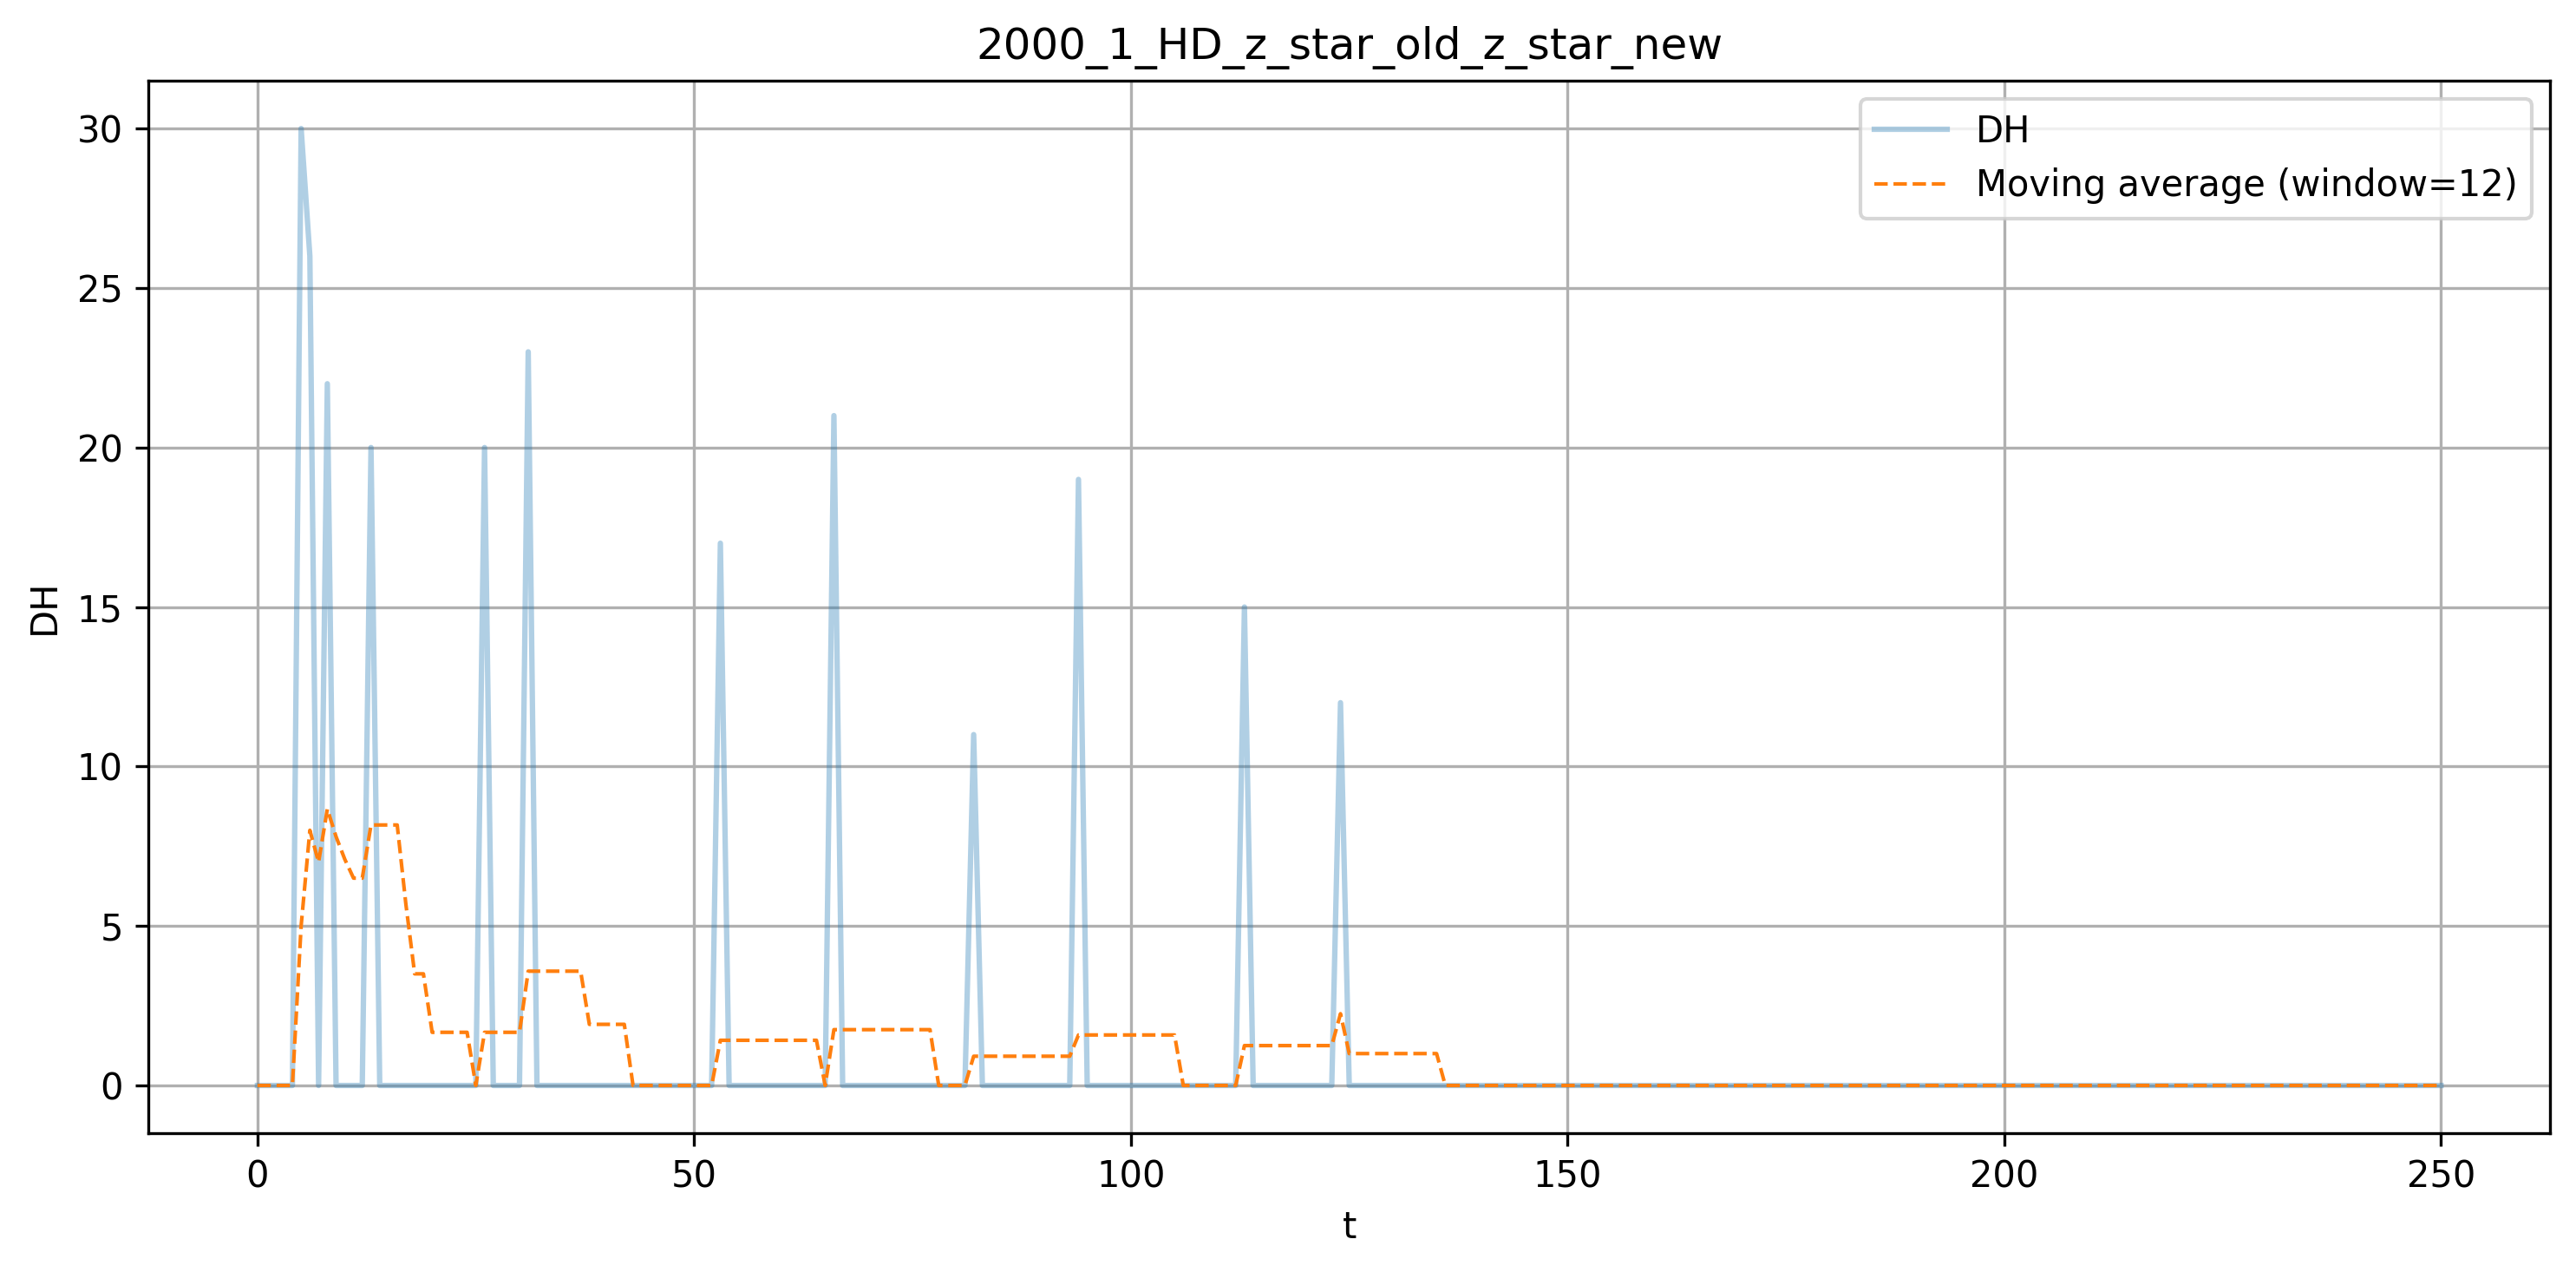
\includegraphics[width=\linewidth]{../Quantum-Annealing-for-solving-QUBO-Problems/test/Lambda_dinamico/ksp_2/lambda_650_dot_C/2000_1_HD_z_star_old_z_star_new.png}
    \caption{\(d_H(z_\star^{old}, z_\star^{new})\) con \(\lambda_1\)}
    \label{fig:hd-zstarold-zstarnew-lambda1}
\end{subfigure}
\hfill
\begin{subfigure}{0.495\textwidth}
    \centering
    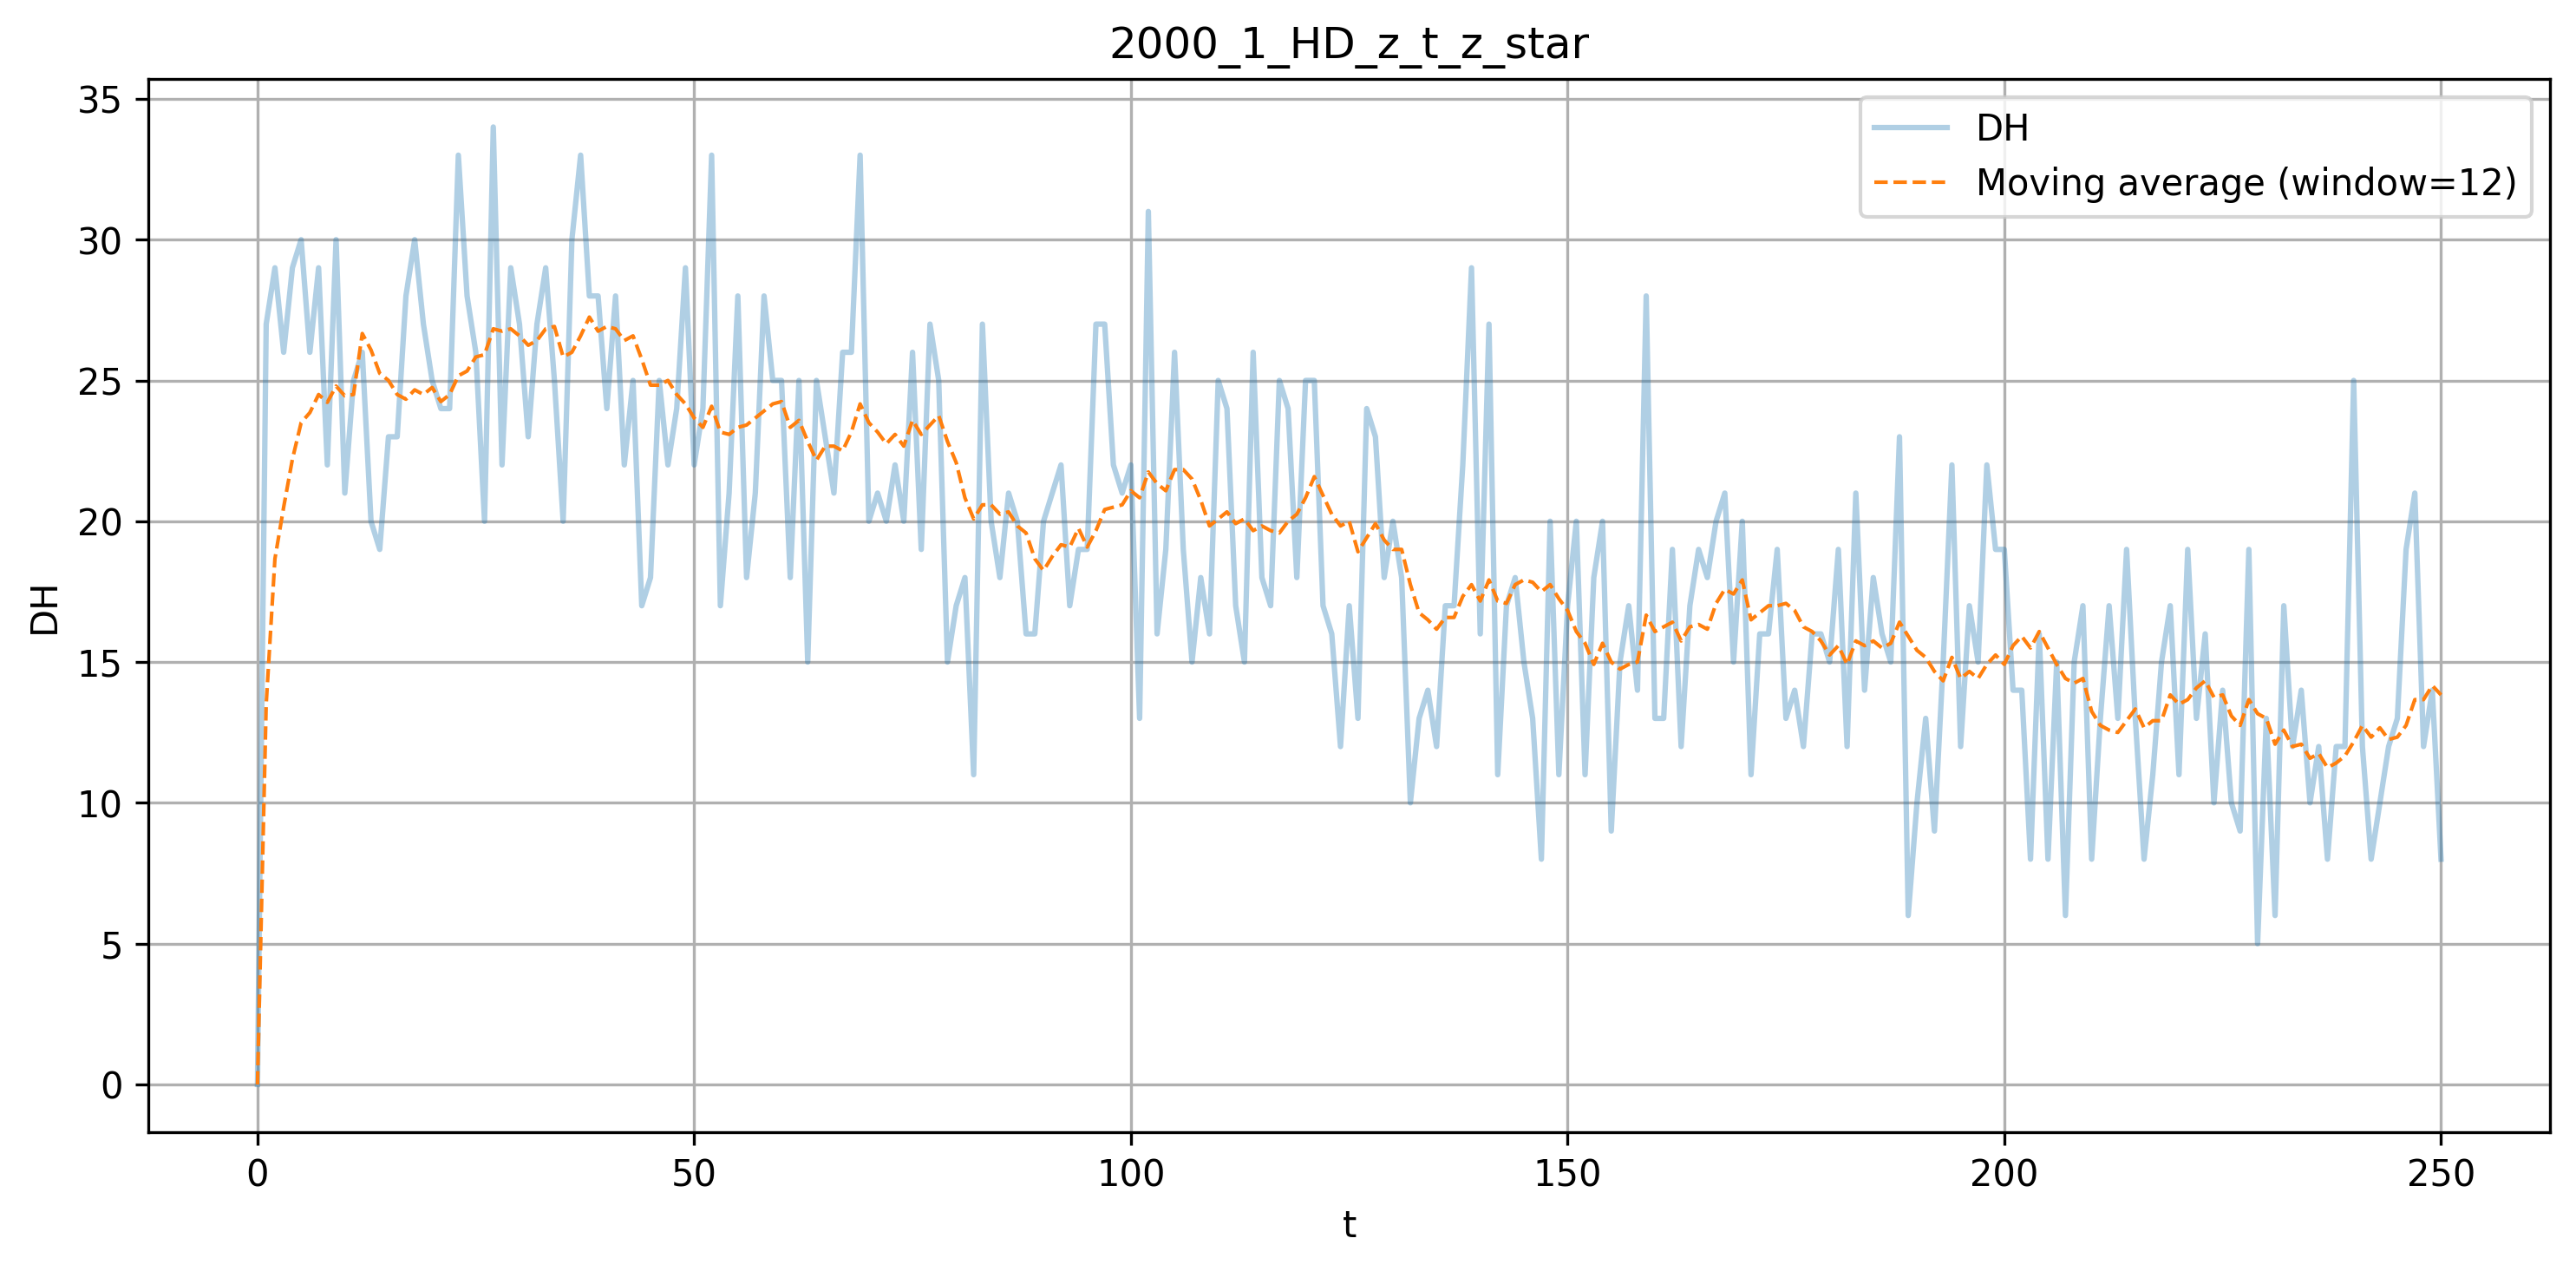
\includegraphics[width=\linewidth]{../Quantum-Annealing-for-solving-QUBO-Problems/test/Lambda_dinamico/ksp_2/lambda_650_dot_C/2000_1_HD_z_t_z_star.png}
    \caption{\(d_H(z_t, z_\star)\) con \(\lambda_1\)}
    \label{fig:hd-zt-zstar-lambda1}
\end{subfigure}

\vspace{0.35cm}

\begin{subfigure}{0.495\textwidth}
    \centering
    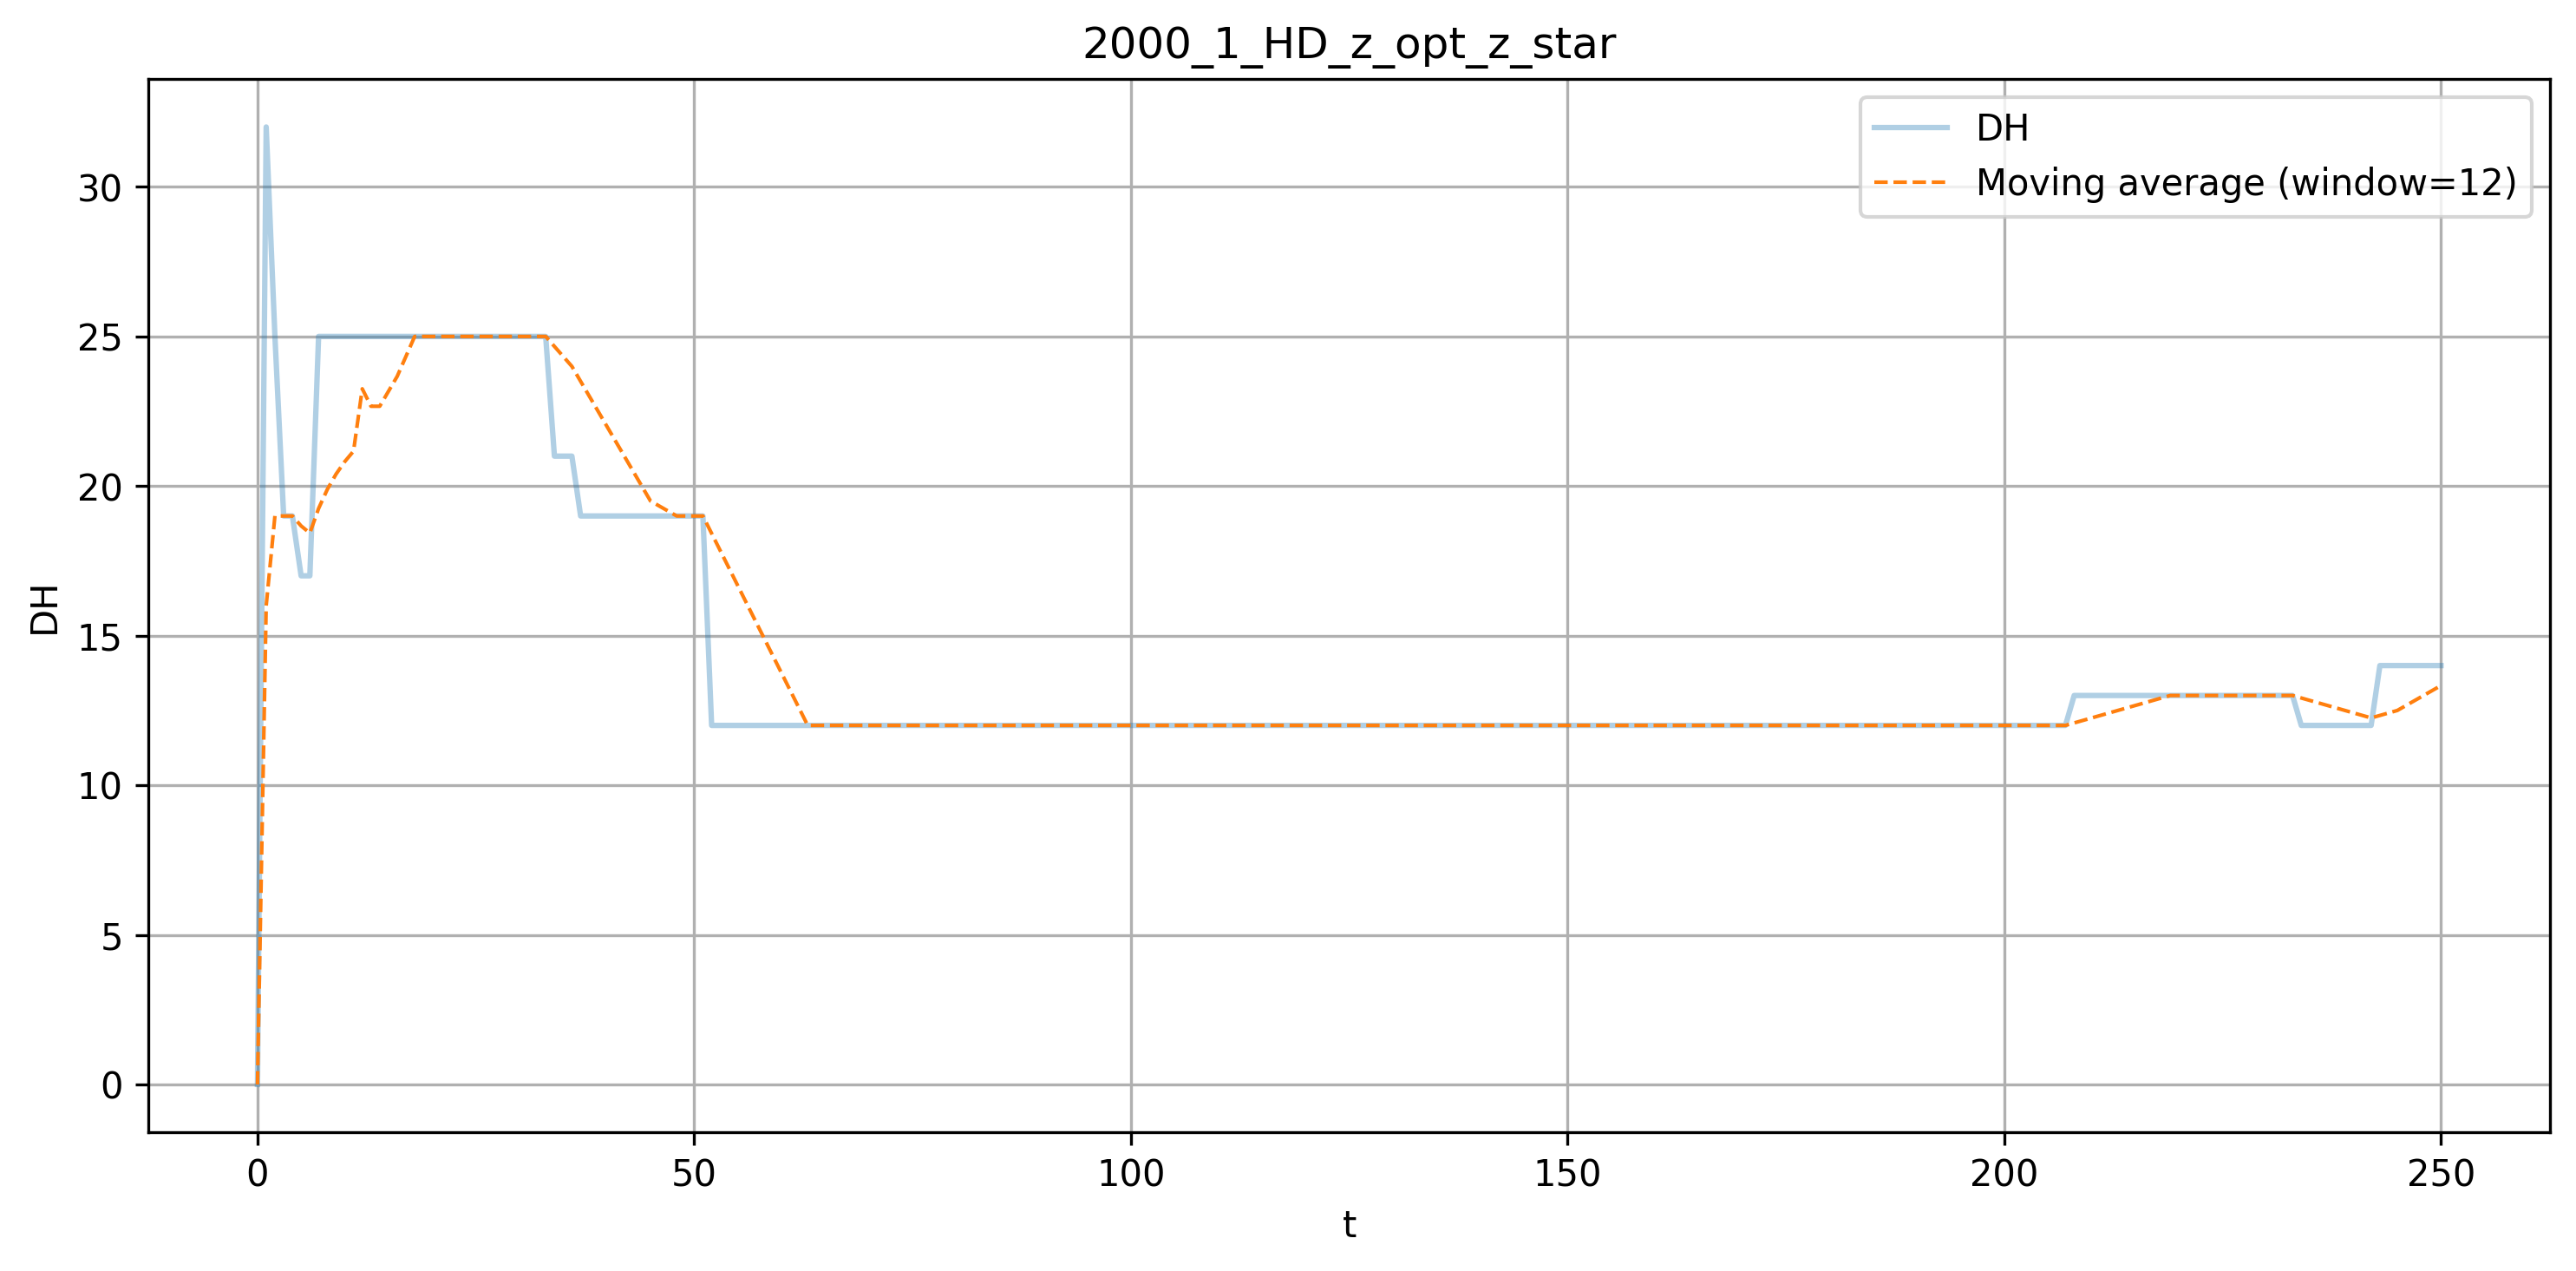
\includegraphics[width=\linewidth]{../Quantum-Annealing-for-solving-QUBO-Problems/test/Lambda_dinamico/ksp_2/lambda_650_dot_C/2000_1_HD_z_opt_z_star.png}
    \caption{\(d_H(z_{opt}, z_\star)\) con \(\lambda_1\)}
    \label{fig:hd-zopt-zstar-lambda1}
\end{subfigure}
\hfill
\begin{subfigure}{0.495\textwidth}
    \centering
    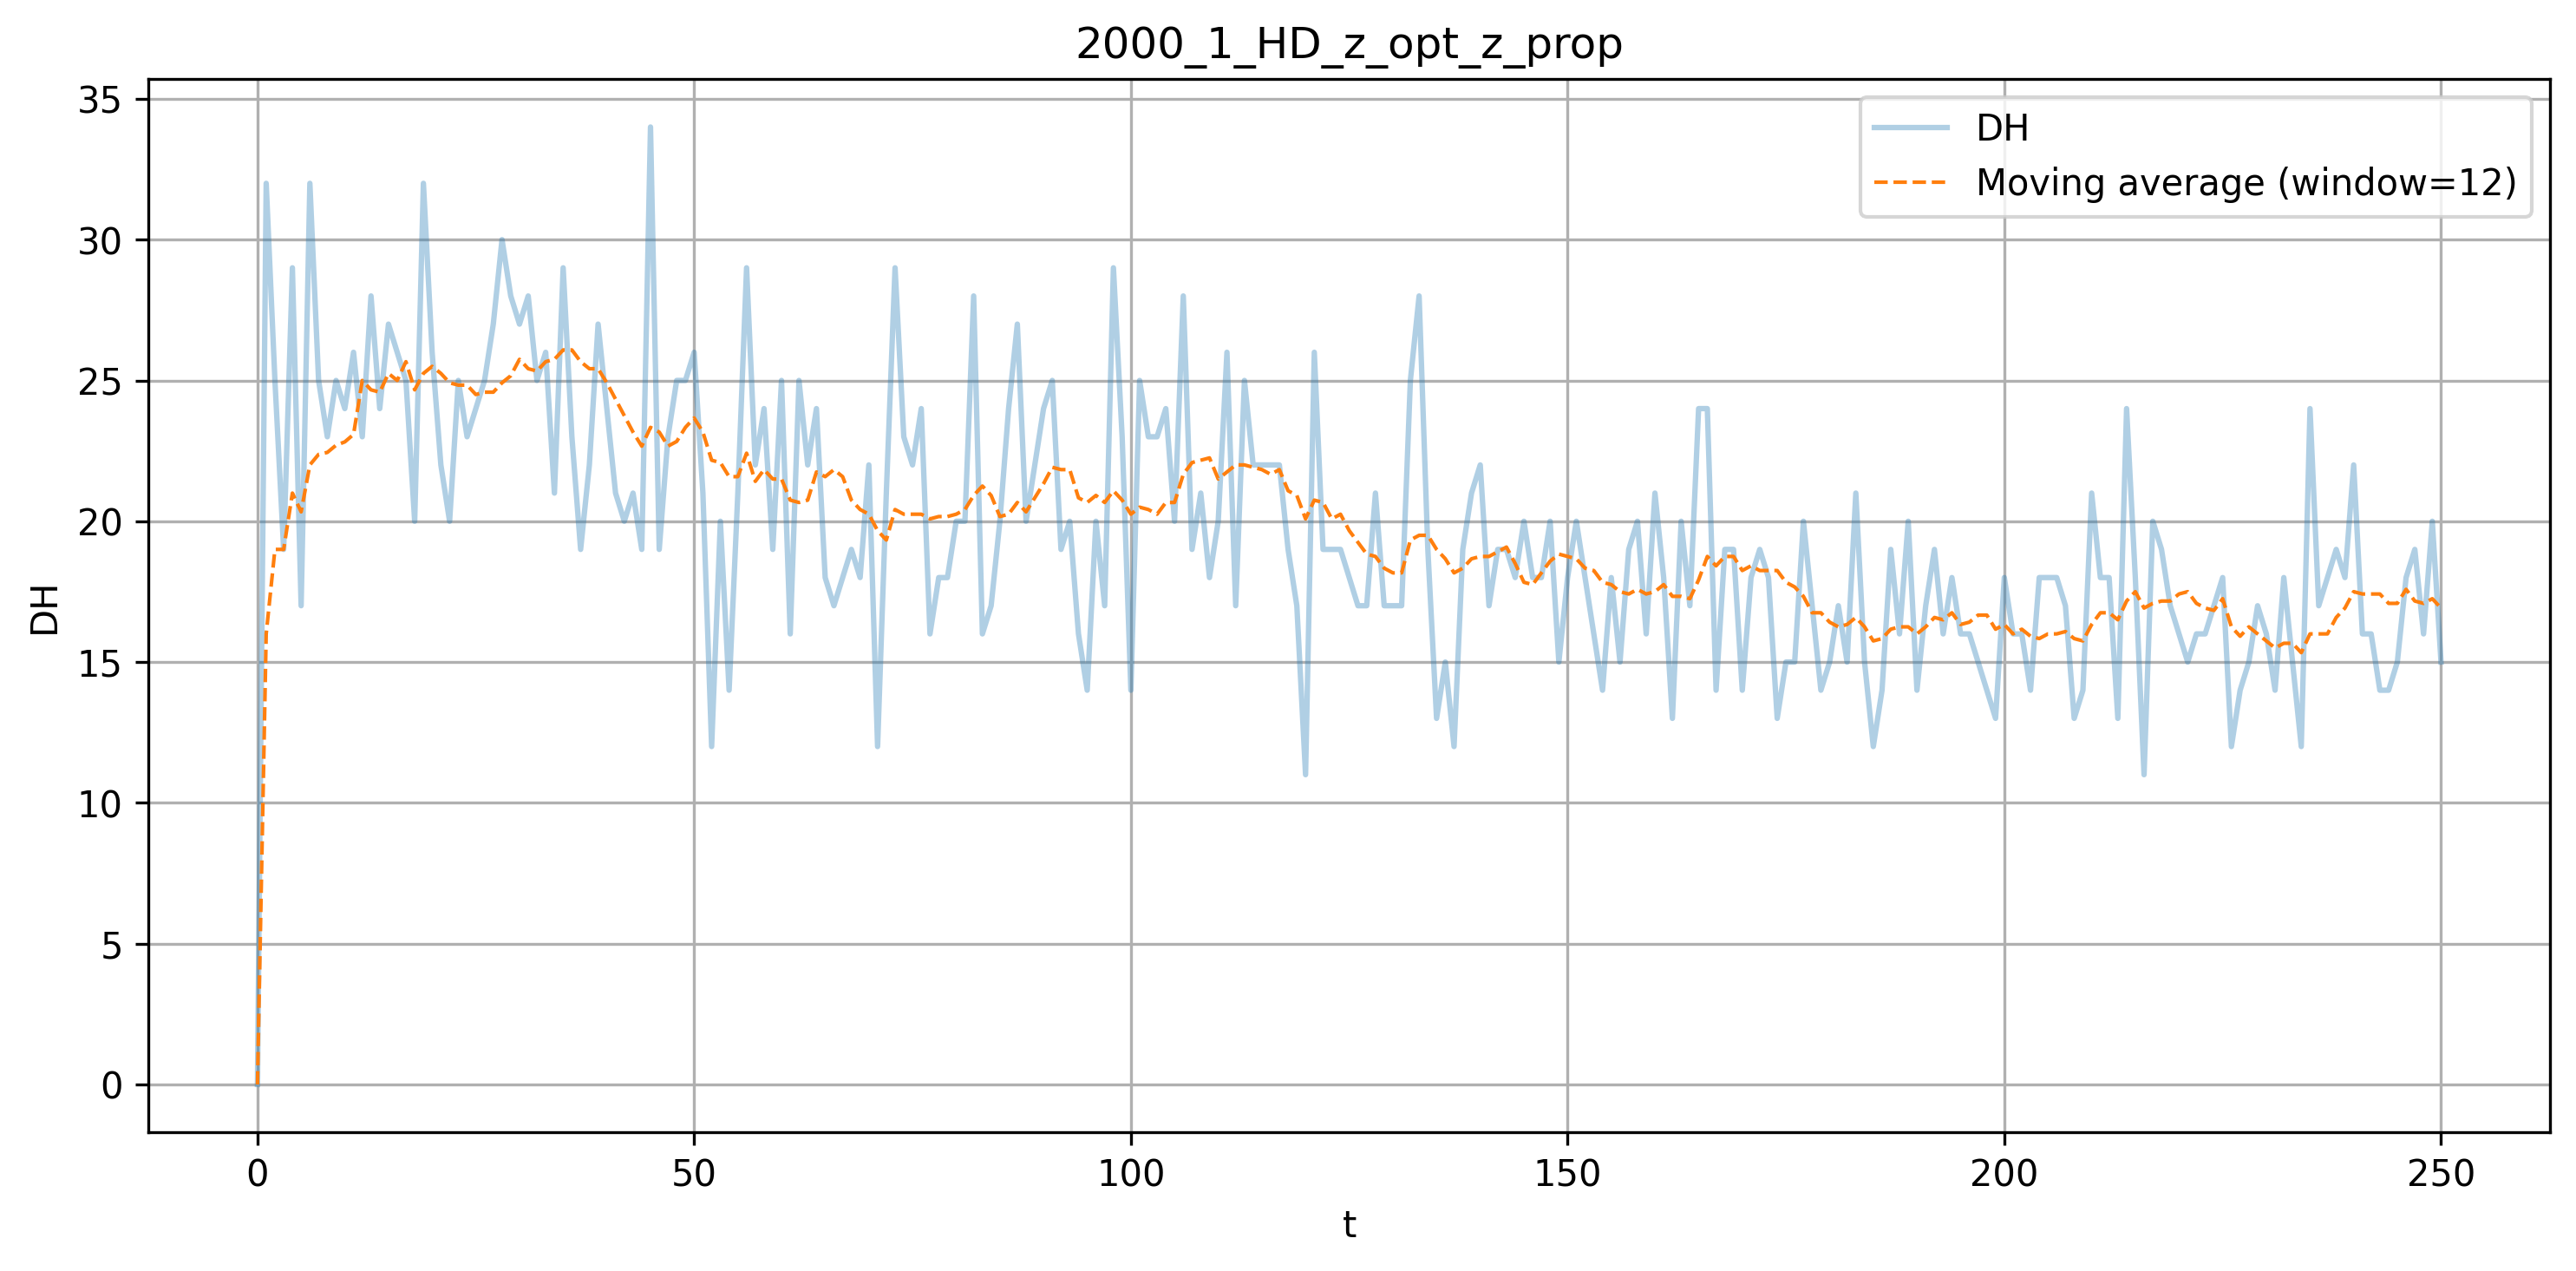
\includegraphics[width=\linewidth]{../Quantum-Annealing-for-solving-QUBO-Problems/test/Lambda_dinamico/ksp_2/lambda_650_dot_C/2000_1_HD_z_opt_z_prop.png}
    \caption{\(d_H(z_{opt}, z_t)\) con \(\lambda_1\)}
    \label{fig:hd-zopt-zt-lambda1}
\end{subfigure}

\vspace{0.35cm}

\begin{subfigure}{0.495\textwidth}
    \centering
    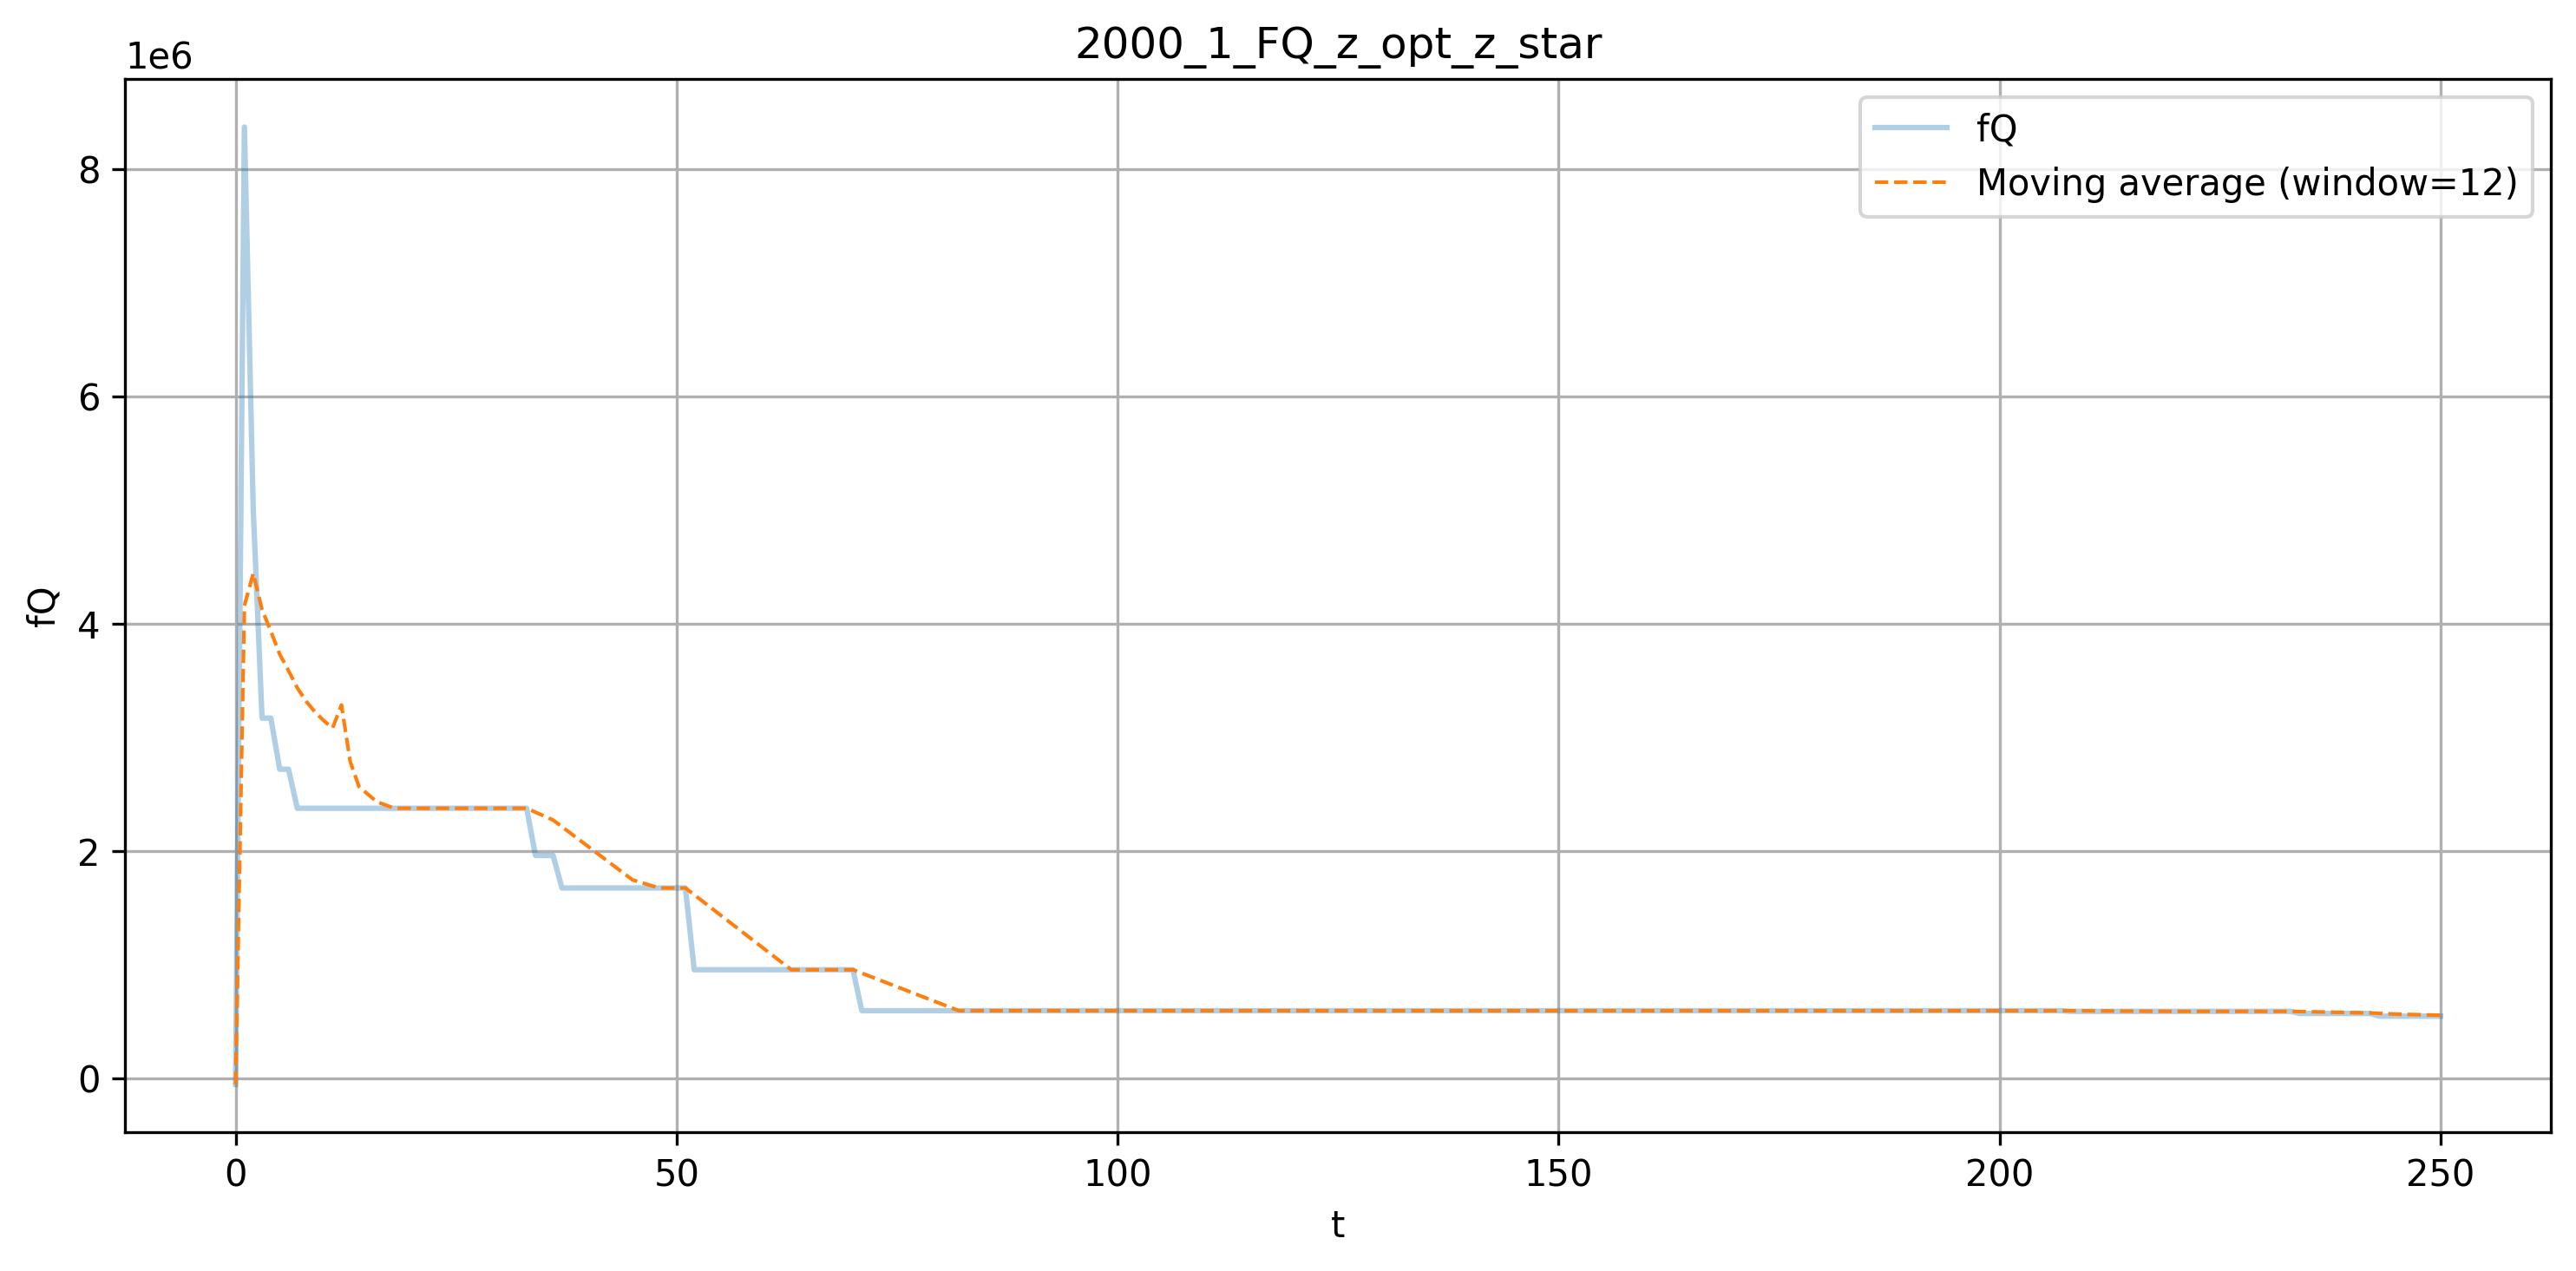
\includegraphics[width=\linewidth]{../Quantum-Annealing-for-solving-QUBO-Problems/test/Lambda_dinamico/ksp_2/lambda_650_dot_C/2000_1_FQ_z_opt_z_star.png}
    \caption{\(f_Q(z_\star)\) con \(\lambda_1\)}
    \label{fig:fQ-zstar-lambda1}
\end{subfigure}
\hfill
\begin{subfigure}{0.495\textwidth}
    \centering
    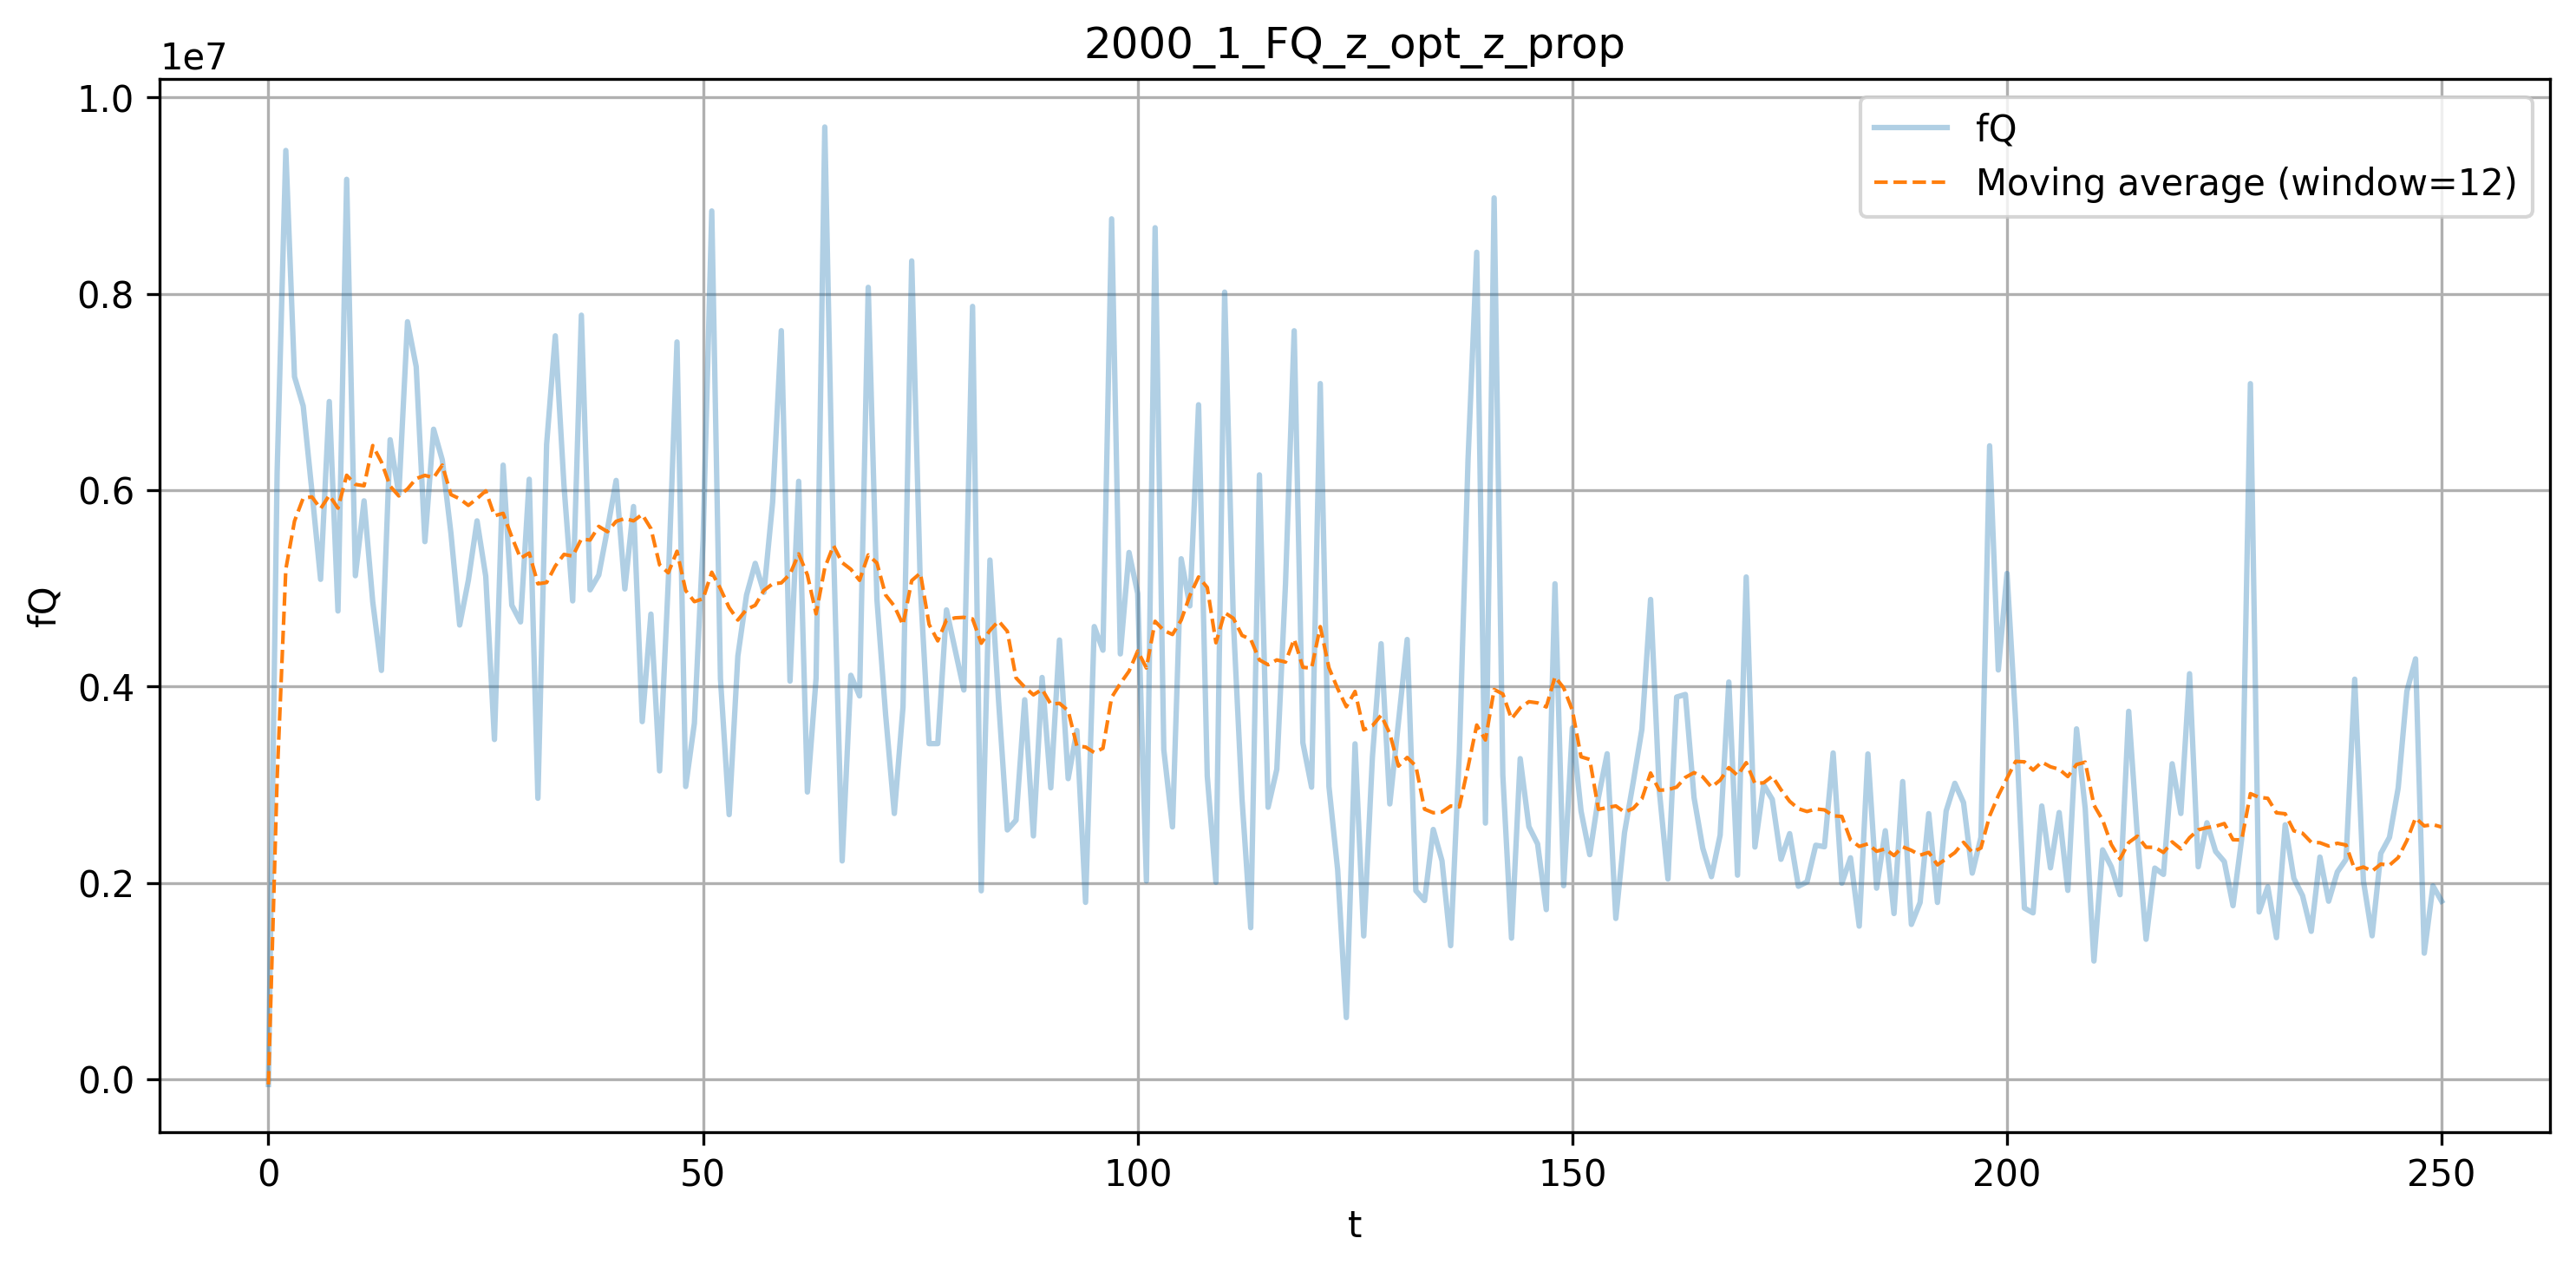
\includegraphics[width=\linewidth]{../Quantum-Annealing-for-solving-QUBO-Problems/test/Lambda_dinamico/ksp_2/lambda_650_dot_C/2000_1_FQ_z_opt_z_prop.png}
    \caption{\(f_Q(z_t)\) con \(\lambda_1\)}
    \label{fig:fQ-zt-lambda1}
\end{subfigure}
\label{fig:confronto-hamming-ksp21}
\end{figure}

\begin{figure}[H]
\centering
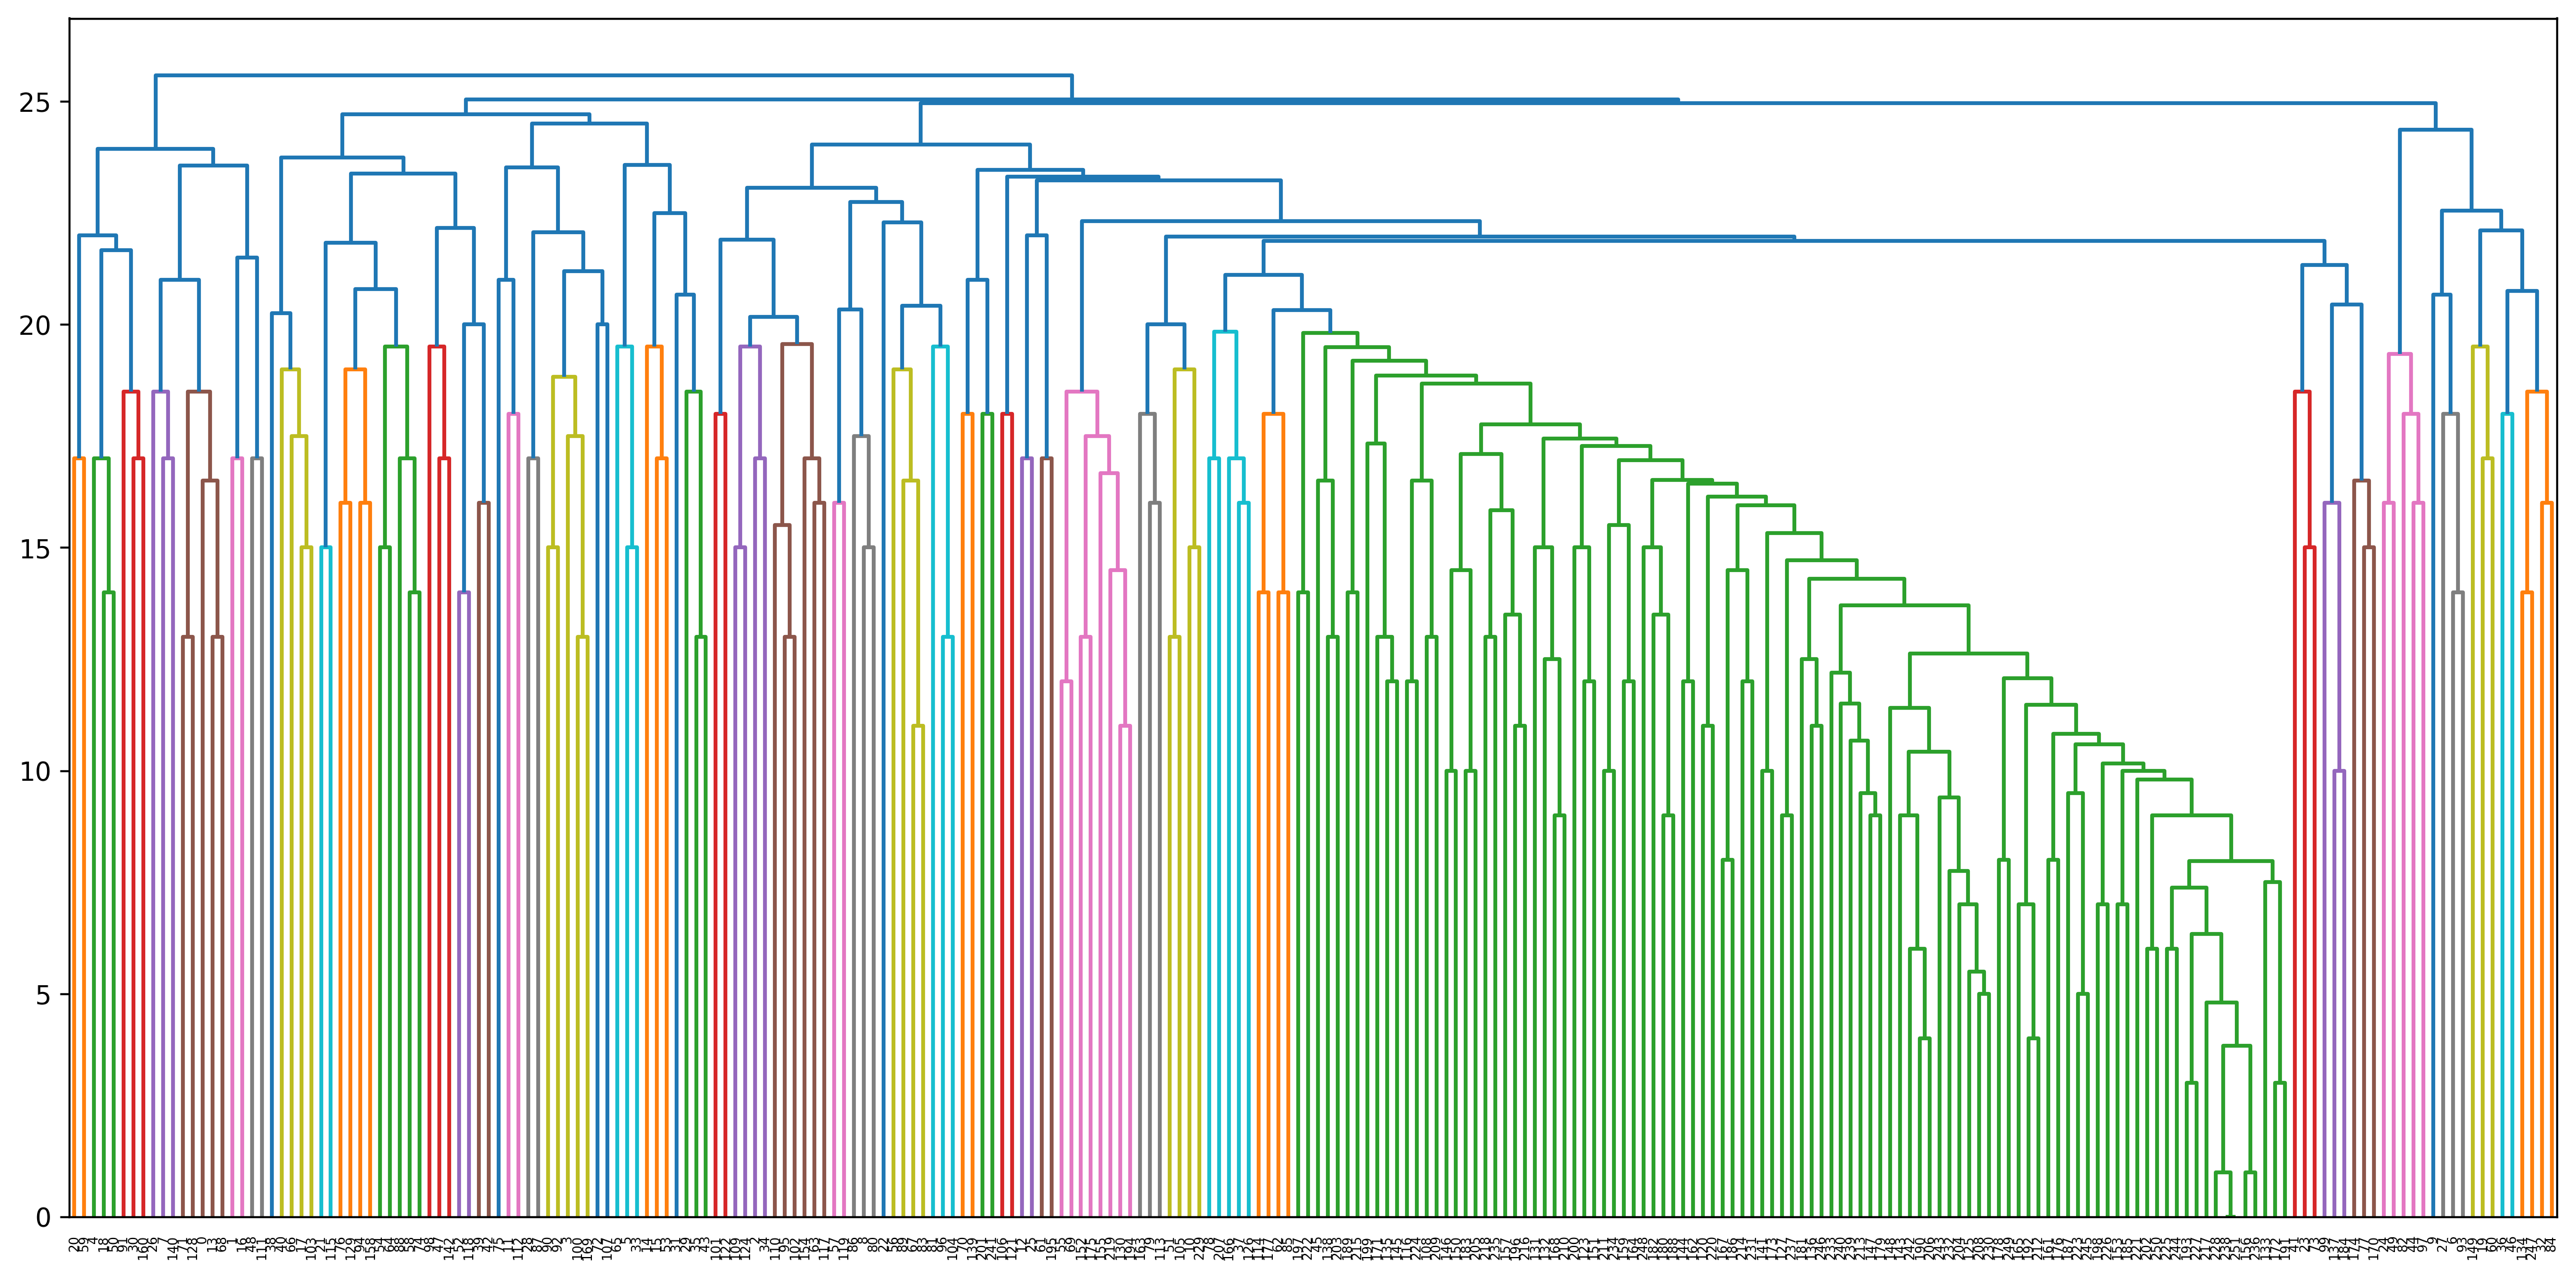
\includegraphics[width=\linewidth]{../Quantum-Annealing-for-solving-QUBO-Problems/test/Lambda_dinamico/ksp_2/lambda_650_dot_C/dendrogram_2000_1.png}
\caption{Agglomerative Clustering Dendogram}
\label{fig:AgglomerativeClustering-ksp2}
\end{figure}

\clearpage
\begin{figure}[H]
\centering
\begin{subfigure}{0.495\textwidth}
    \centering
    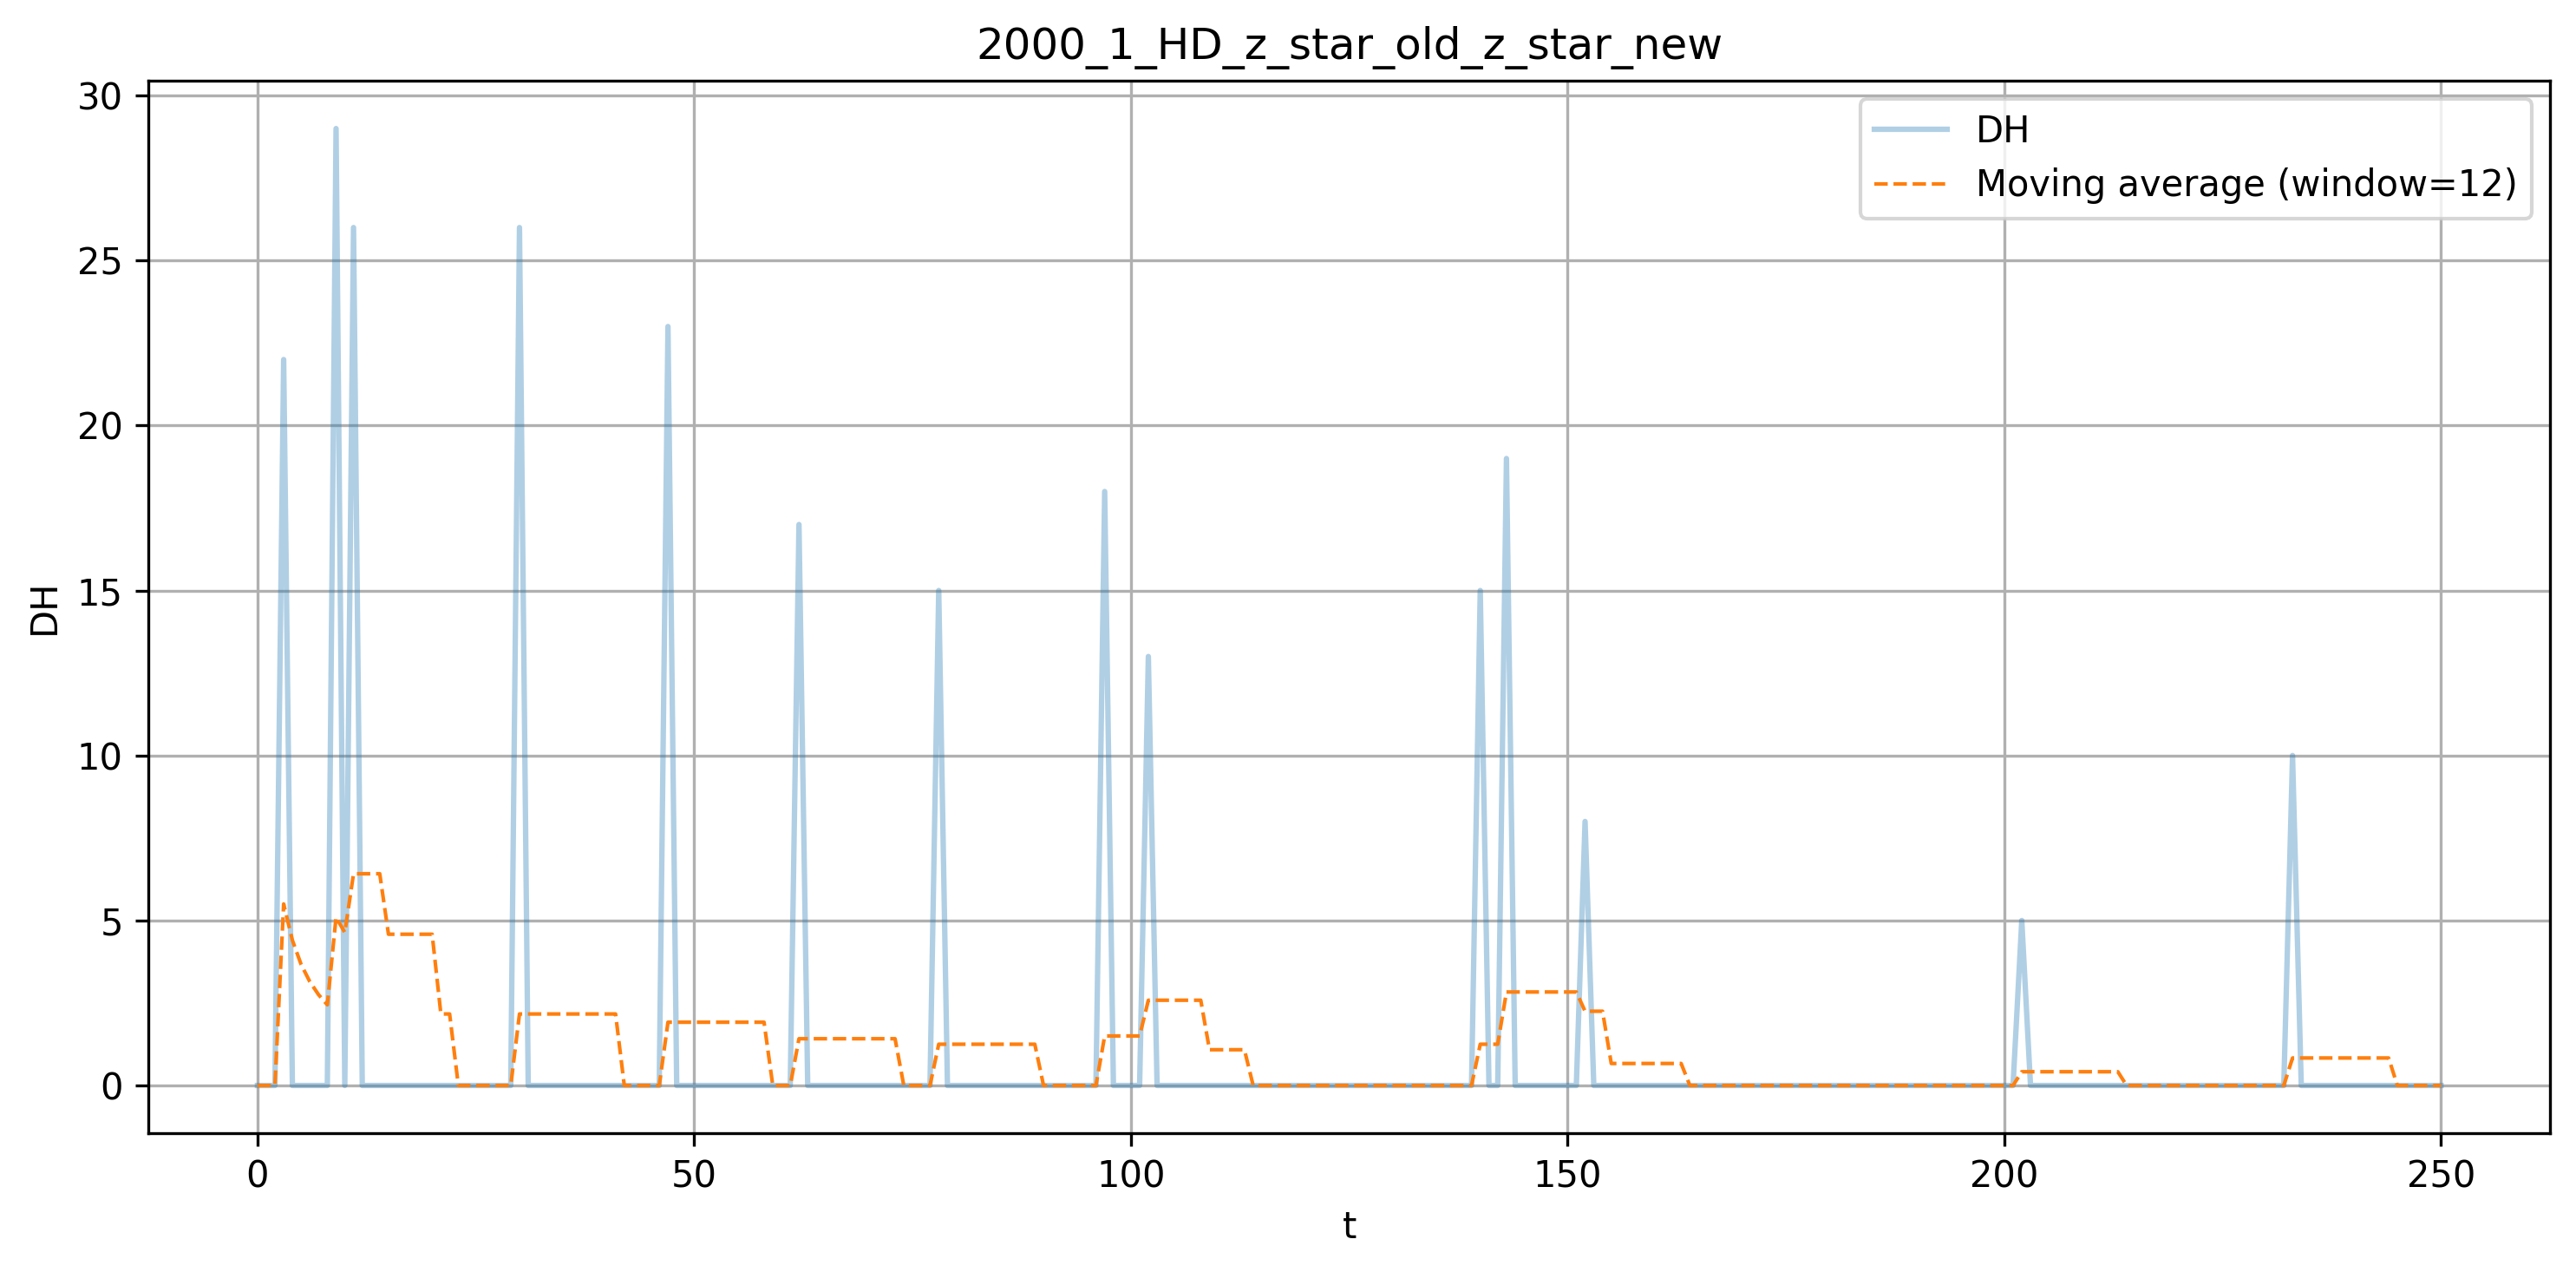
\includegraphics[width=\linewidth]{../Quantum-Annealing-for-solving-QUBO-Problems/test/Lambda_dinamico/ksp_2/lambda_div_3/2000_1_HD_z_star_old_z_star_new.png}
    \caption{\(d_H(z_\star^{old}, z_\star^{new})\) con \(\lambda_2\)}
    \label{fig:hd-zstarold-zstarnew-lambda2}
\end{subfigure}
\hfill
\begin{subfigure}{0.495\textwidth}
    \centering
    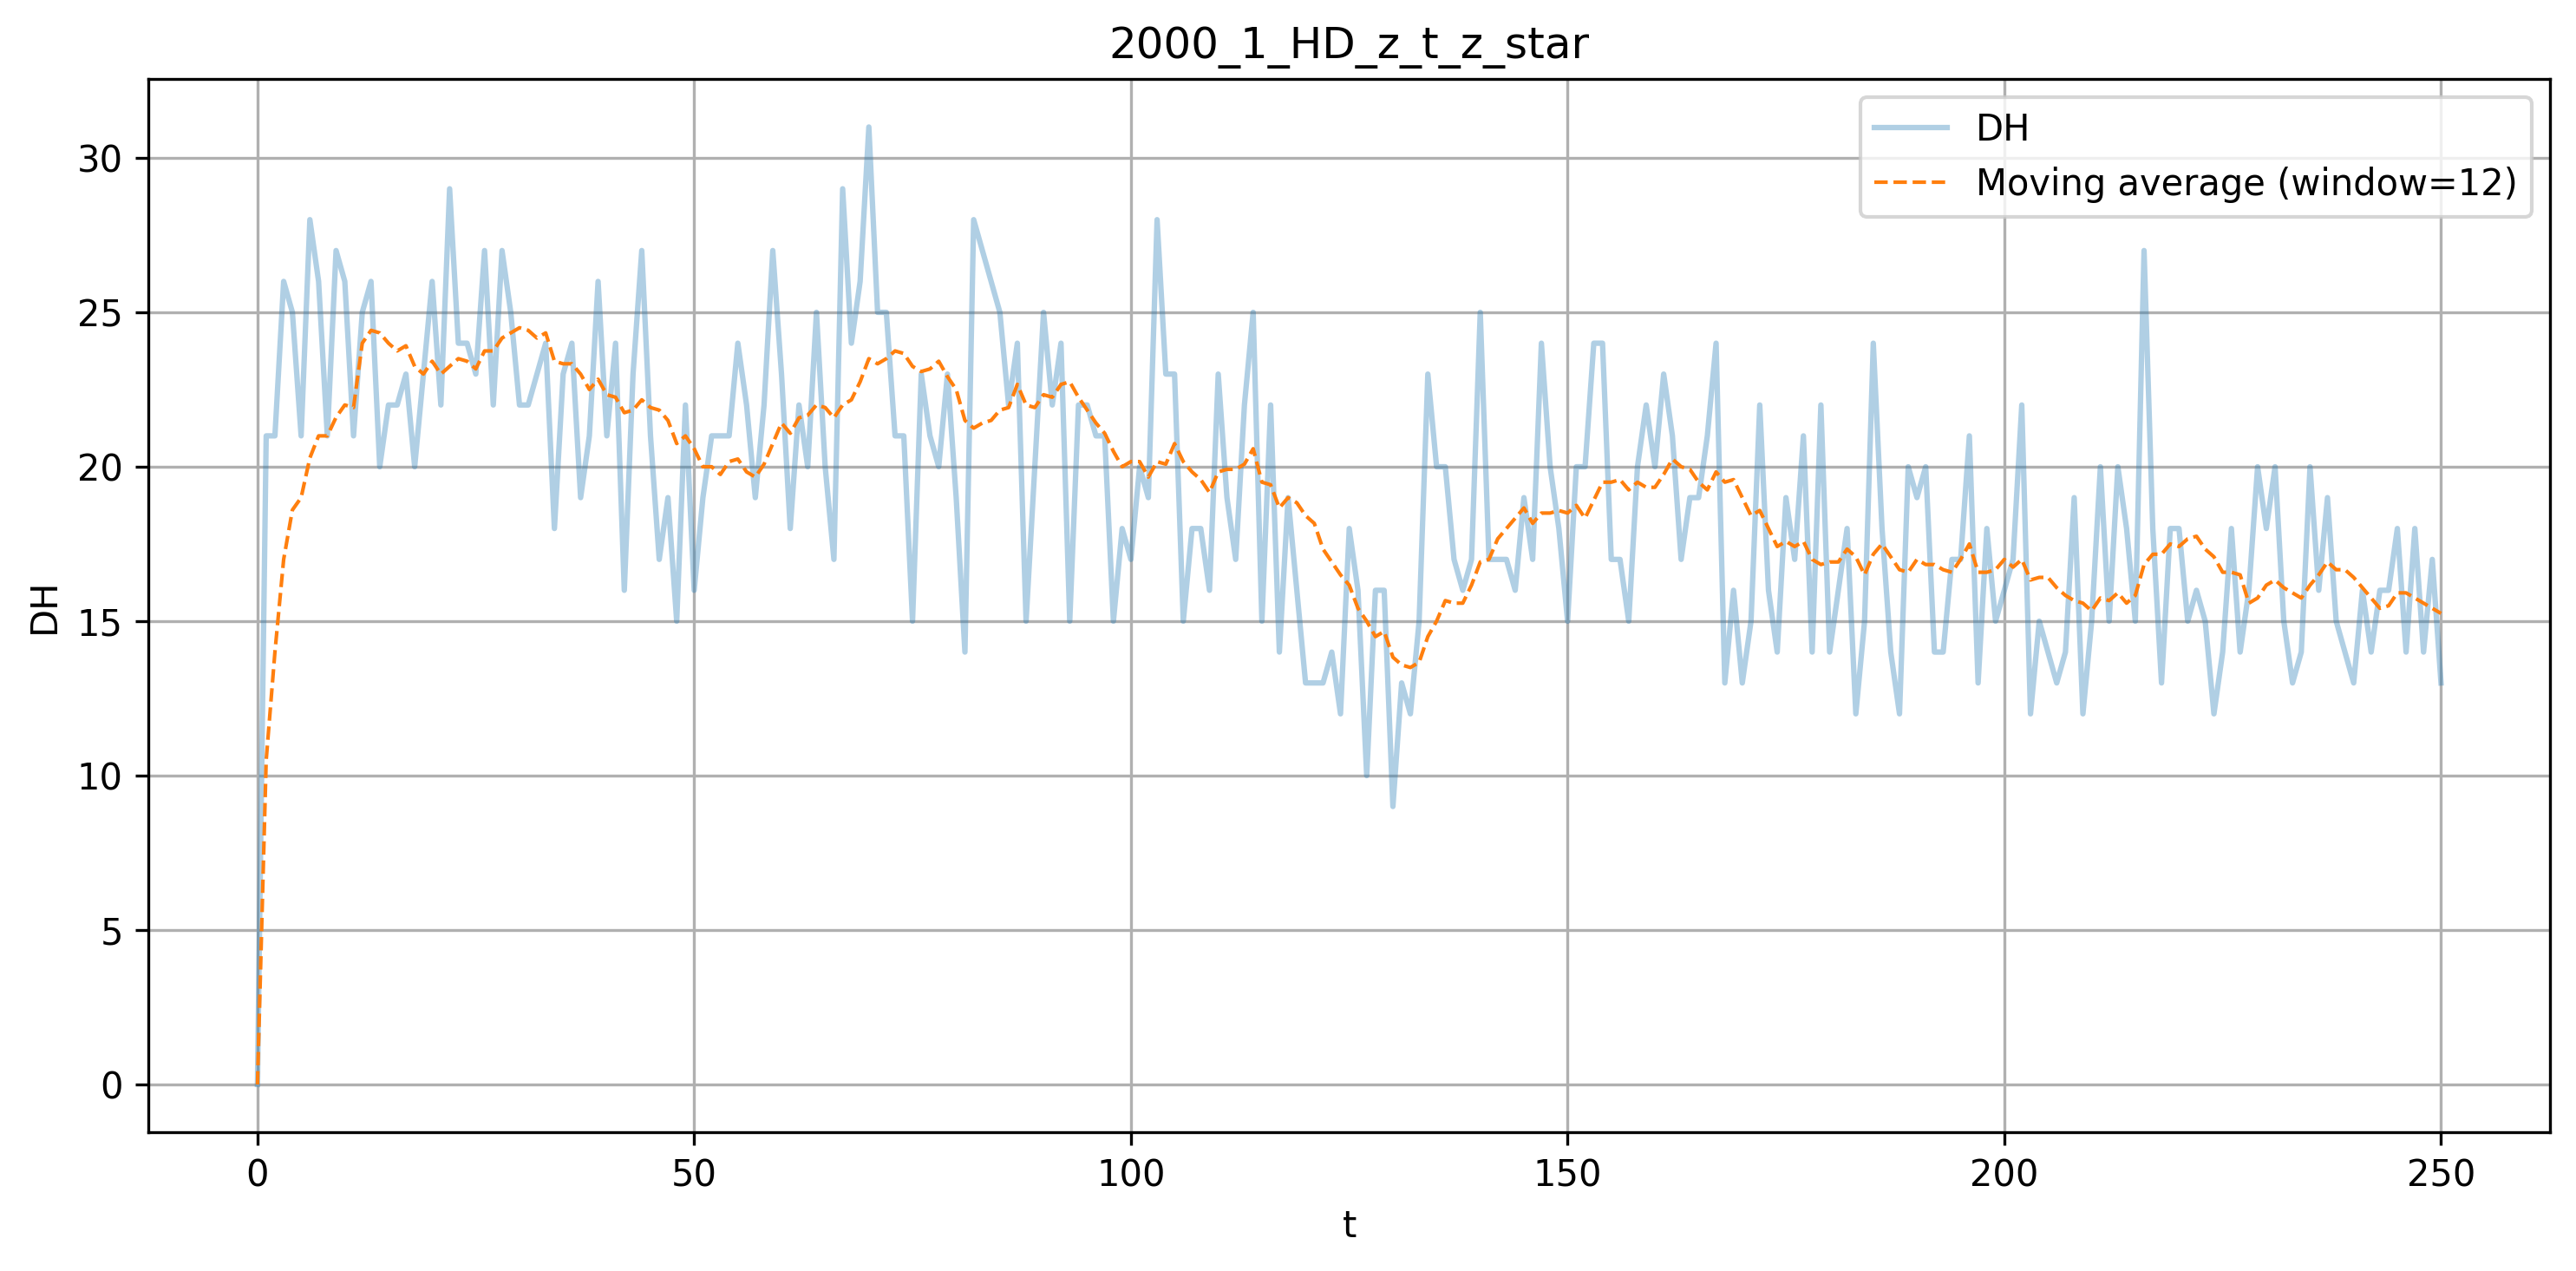
\includegraphics[width=\linewidth]{../Quantum-Annealing-for-solving-QUBO-Problems/test/Lambda_dinamico/ksp_2/lambda_div_3/2000_1_HD_z_t_z_star.png}
    \caption{\(d_H(z_t, z_\star)\) con \(\lambda_2\)}
    \label{fig:hd-zt-zstar-lambda2}
\end{subfigure}

\vspace{0.35cm}

\begin{subfigure}{0.495\textwidth}
    \centering
    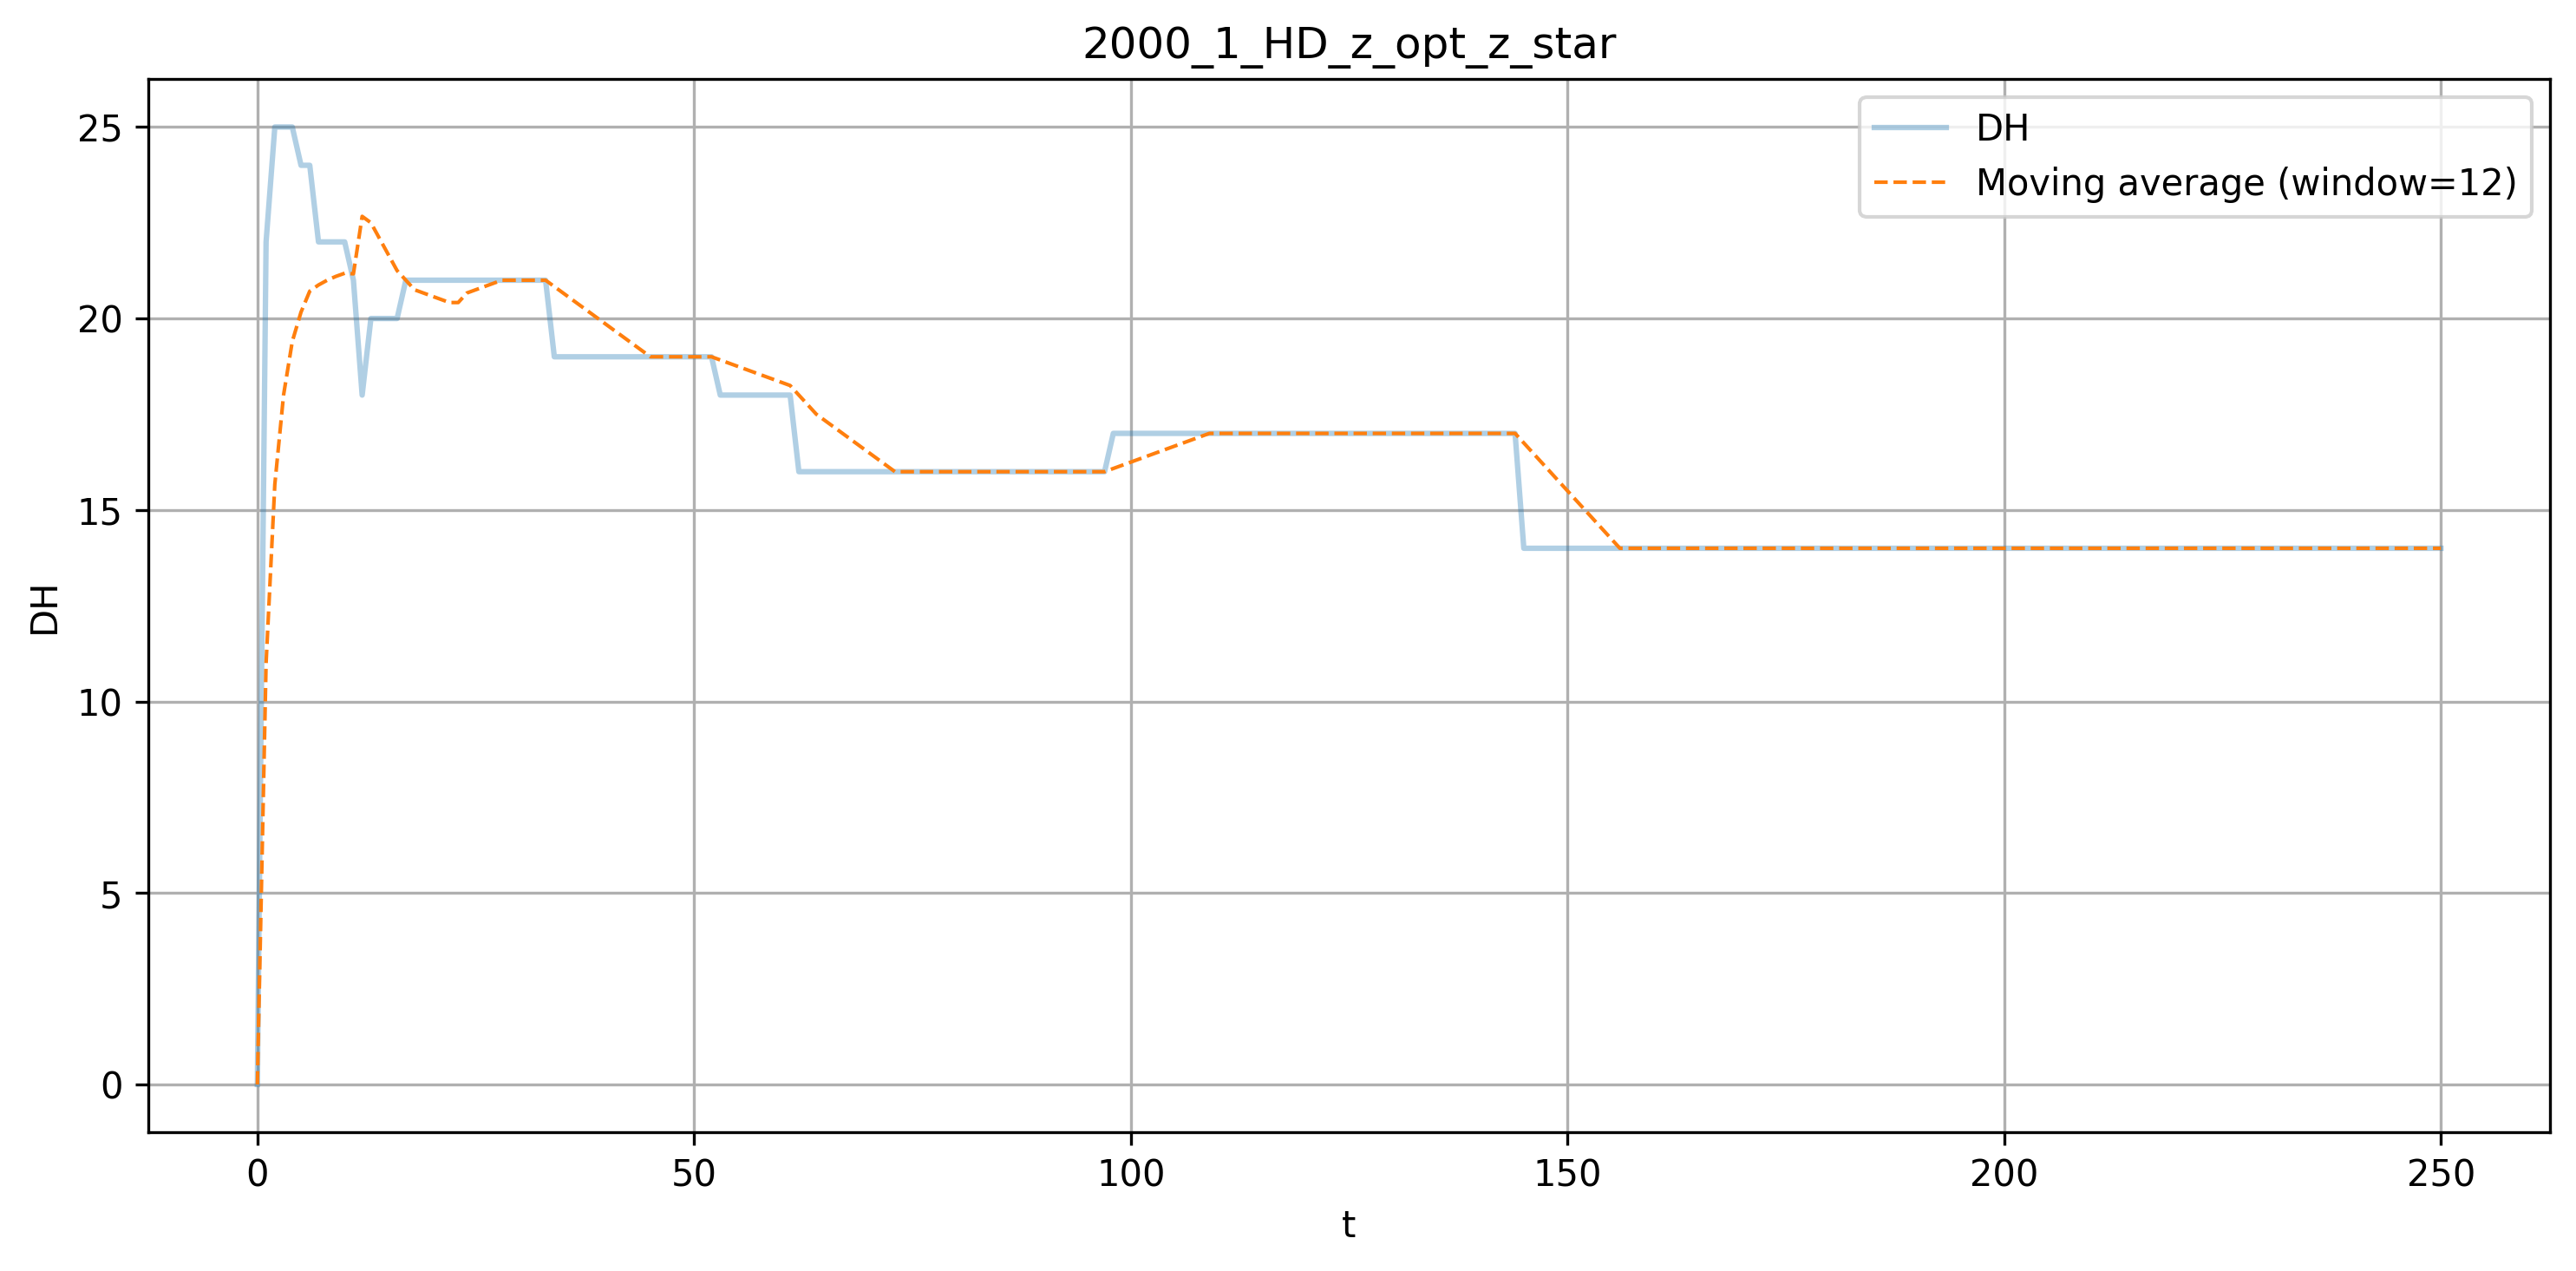
\includegraphics[width=\linewidth]{../Quantum-Annealing-for-solving-QUBO-Problems/test/Lambda_dinamico/ksp_2/lambda_div_3/2000_1_HD_z_opt_z_star.png}
    \caption{\(d_H(z_{opt}, z_\star)\) con \(\lambda_2\)}
    \label{fig:hd-zopt-zstar-lambda2}
\end{subfigure}
\hfill
\begin{subfigure}{0.495\textwidth}
    \centering
    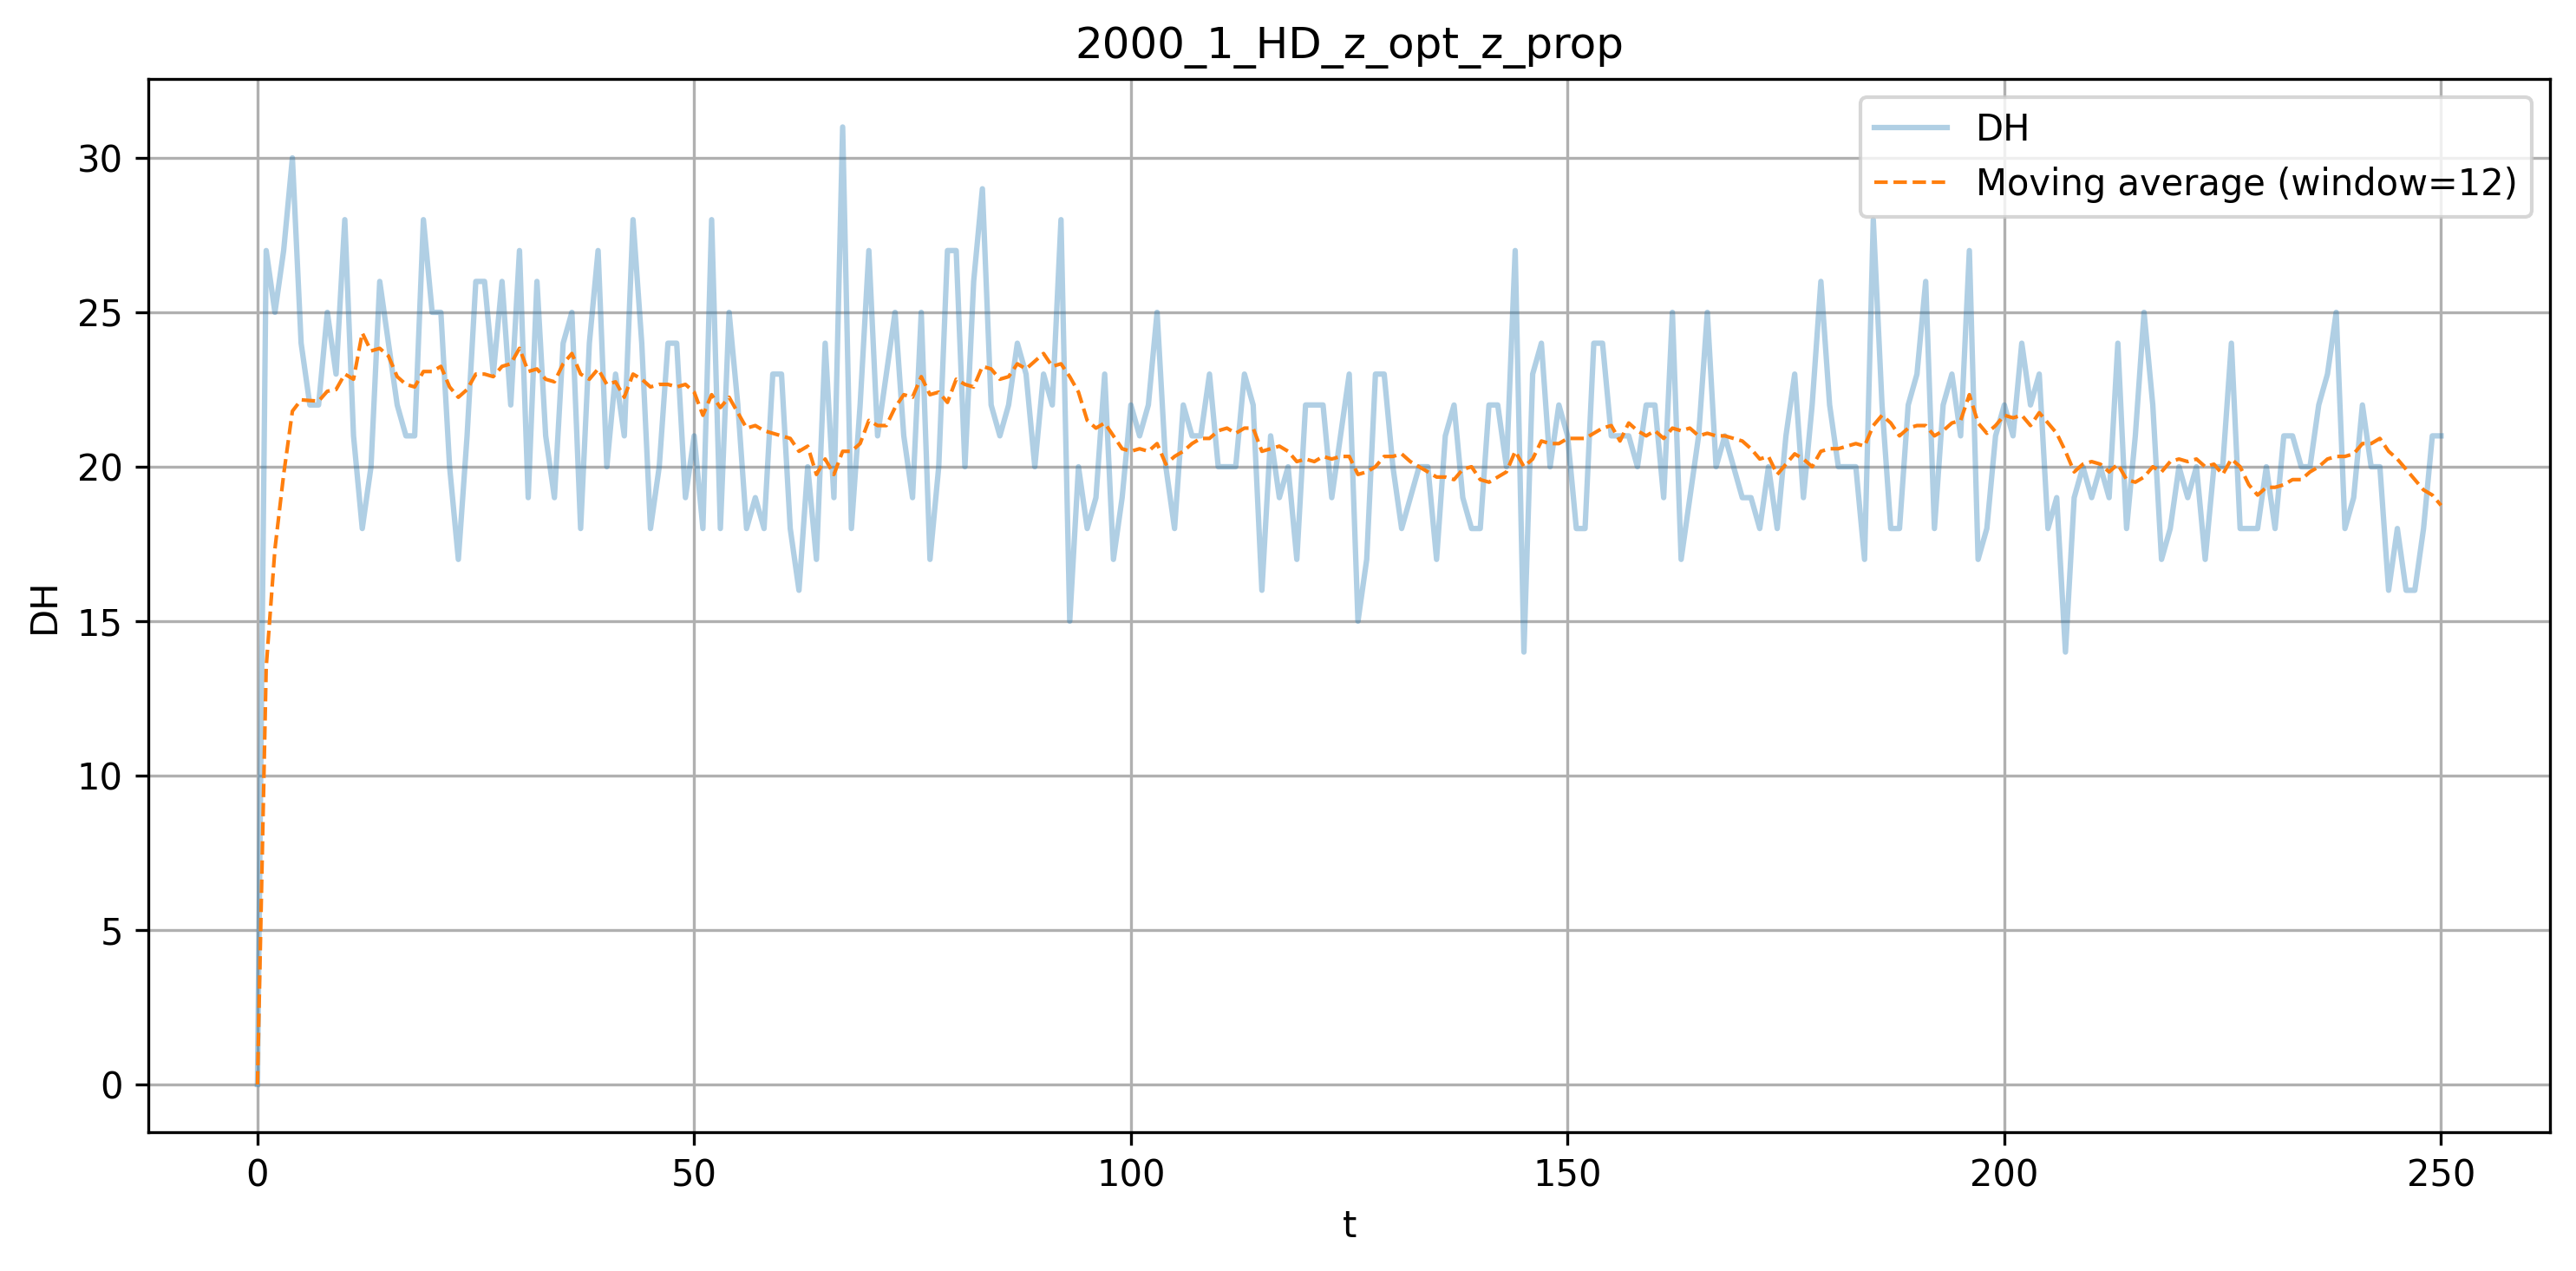
\includegraphics[width=\linewidth]{../Quantum-Annealing-for-solving-QUBO-Problems/test/Lambda_dinamico/ksp_2/lambda_div_3/2000_1_HD_z_opt_z_prop.png}
    \caption{\(d_H(z_{opt}, z_t)\) con \(\lambda_2\)}
    \label{fig:hd-zopt-zt-lambda2}
\end{subfigure}

\vspace{0.35cm}

\begin{subfigure}{0.495\textwidth}
    \centering
    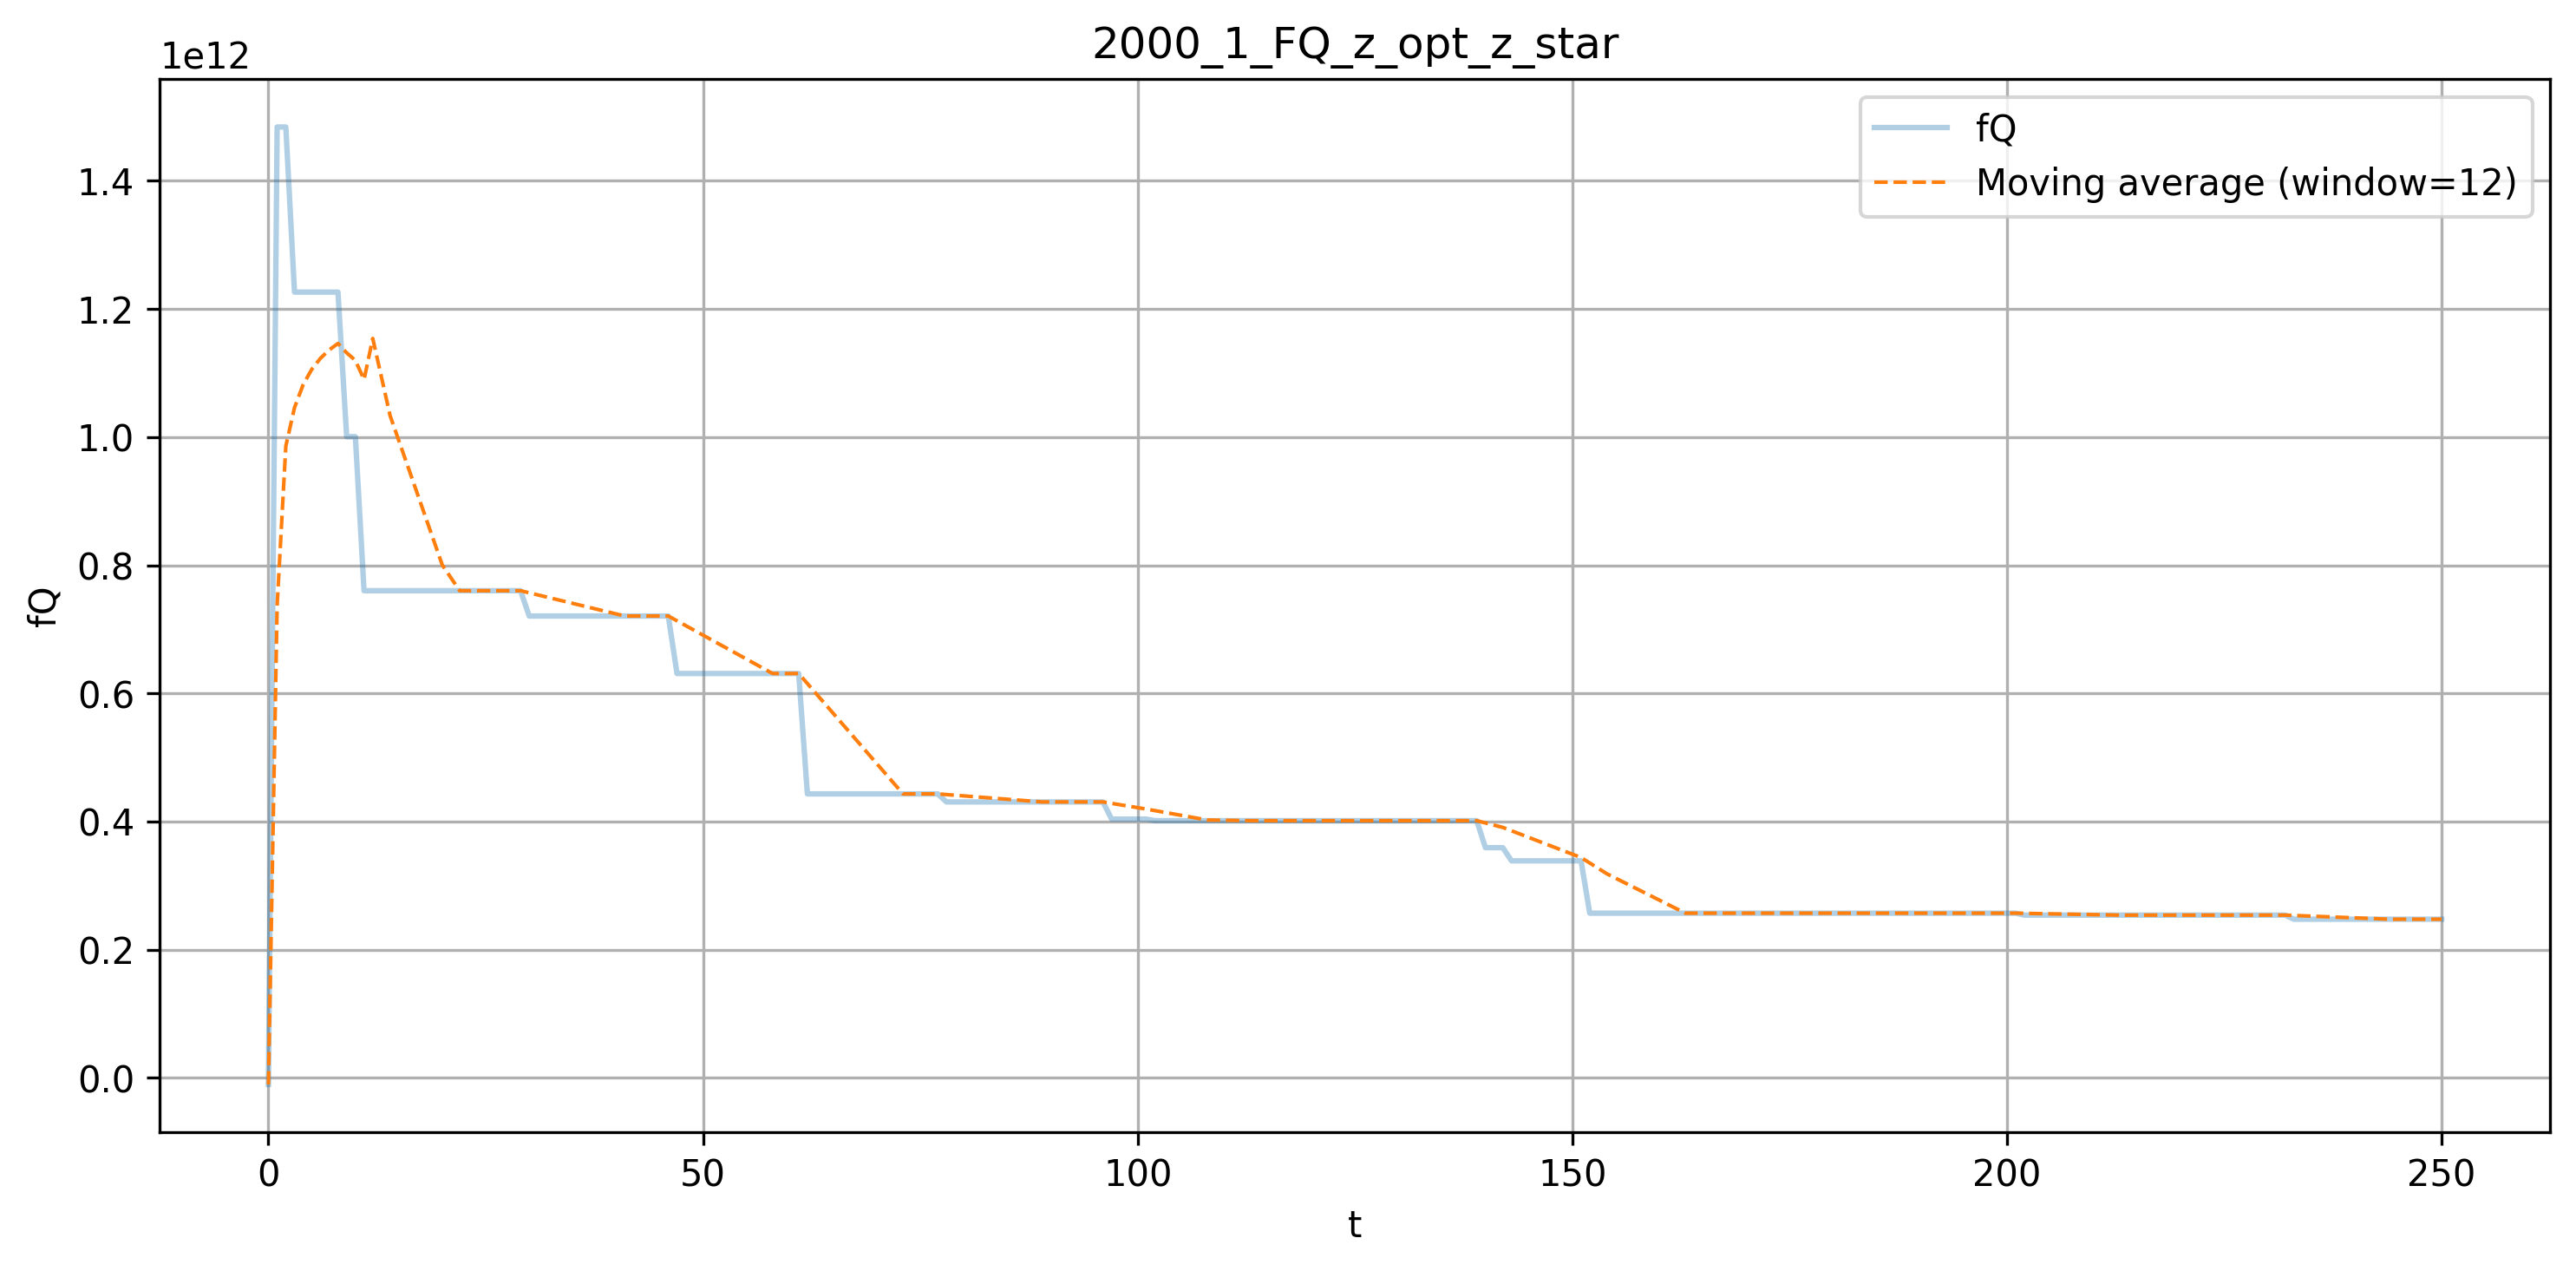
\includegraphics[width=\linewidth]{../Quantum-Annealing-for-solving-QUBO-Problems/test/Lambda_dinamico/ksp_2/lambda_div_3/2000_1_FQ_z_opt_z_star.png}
    \caption{\(f_Q(z_\star)\) con \(\lambda_2\)}
    \label{fig:fQ-zstar-lambda2}
\end{subfigure}
\hfill
\begin{subfigure}{0.495\textwidth}
    \centering
    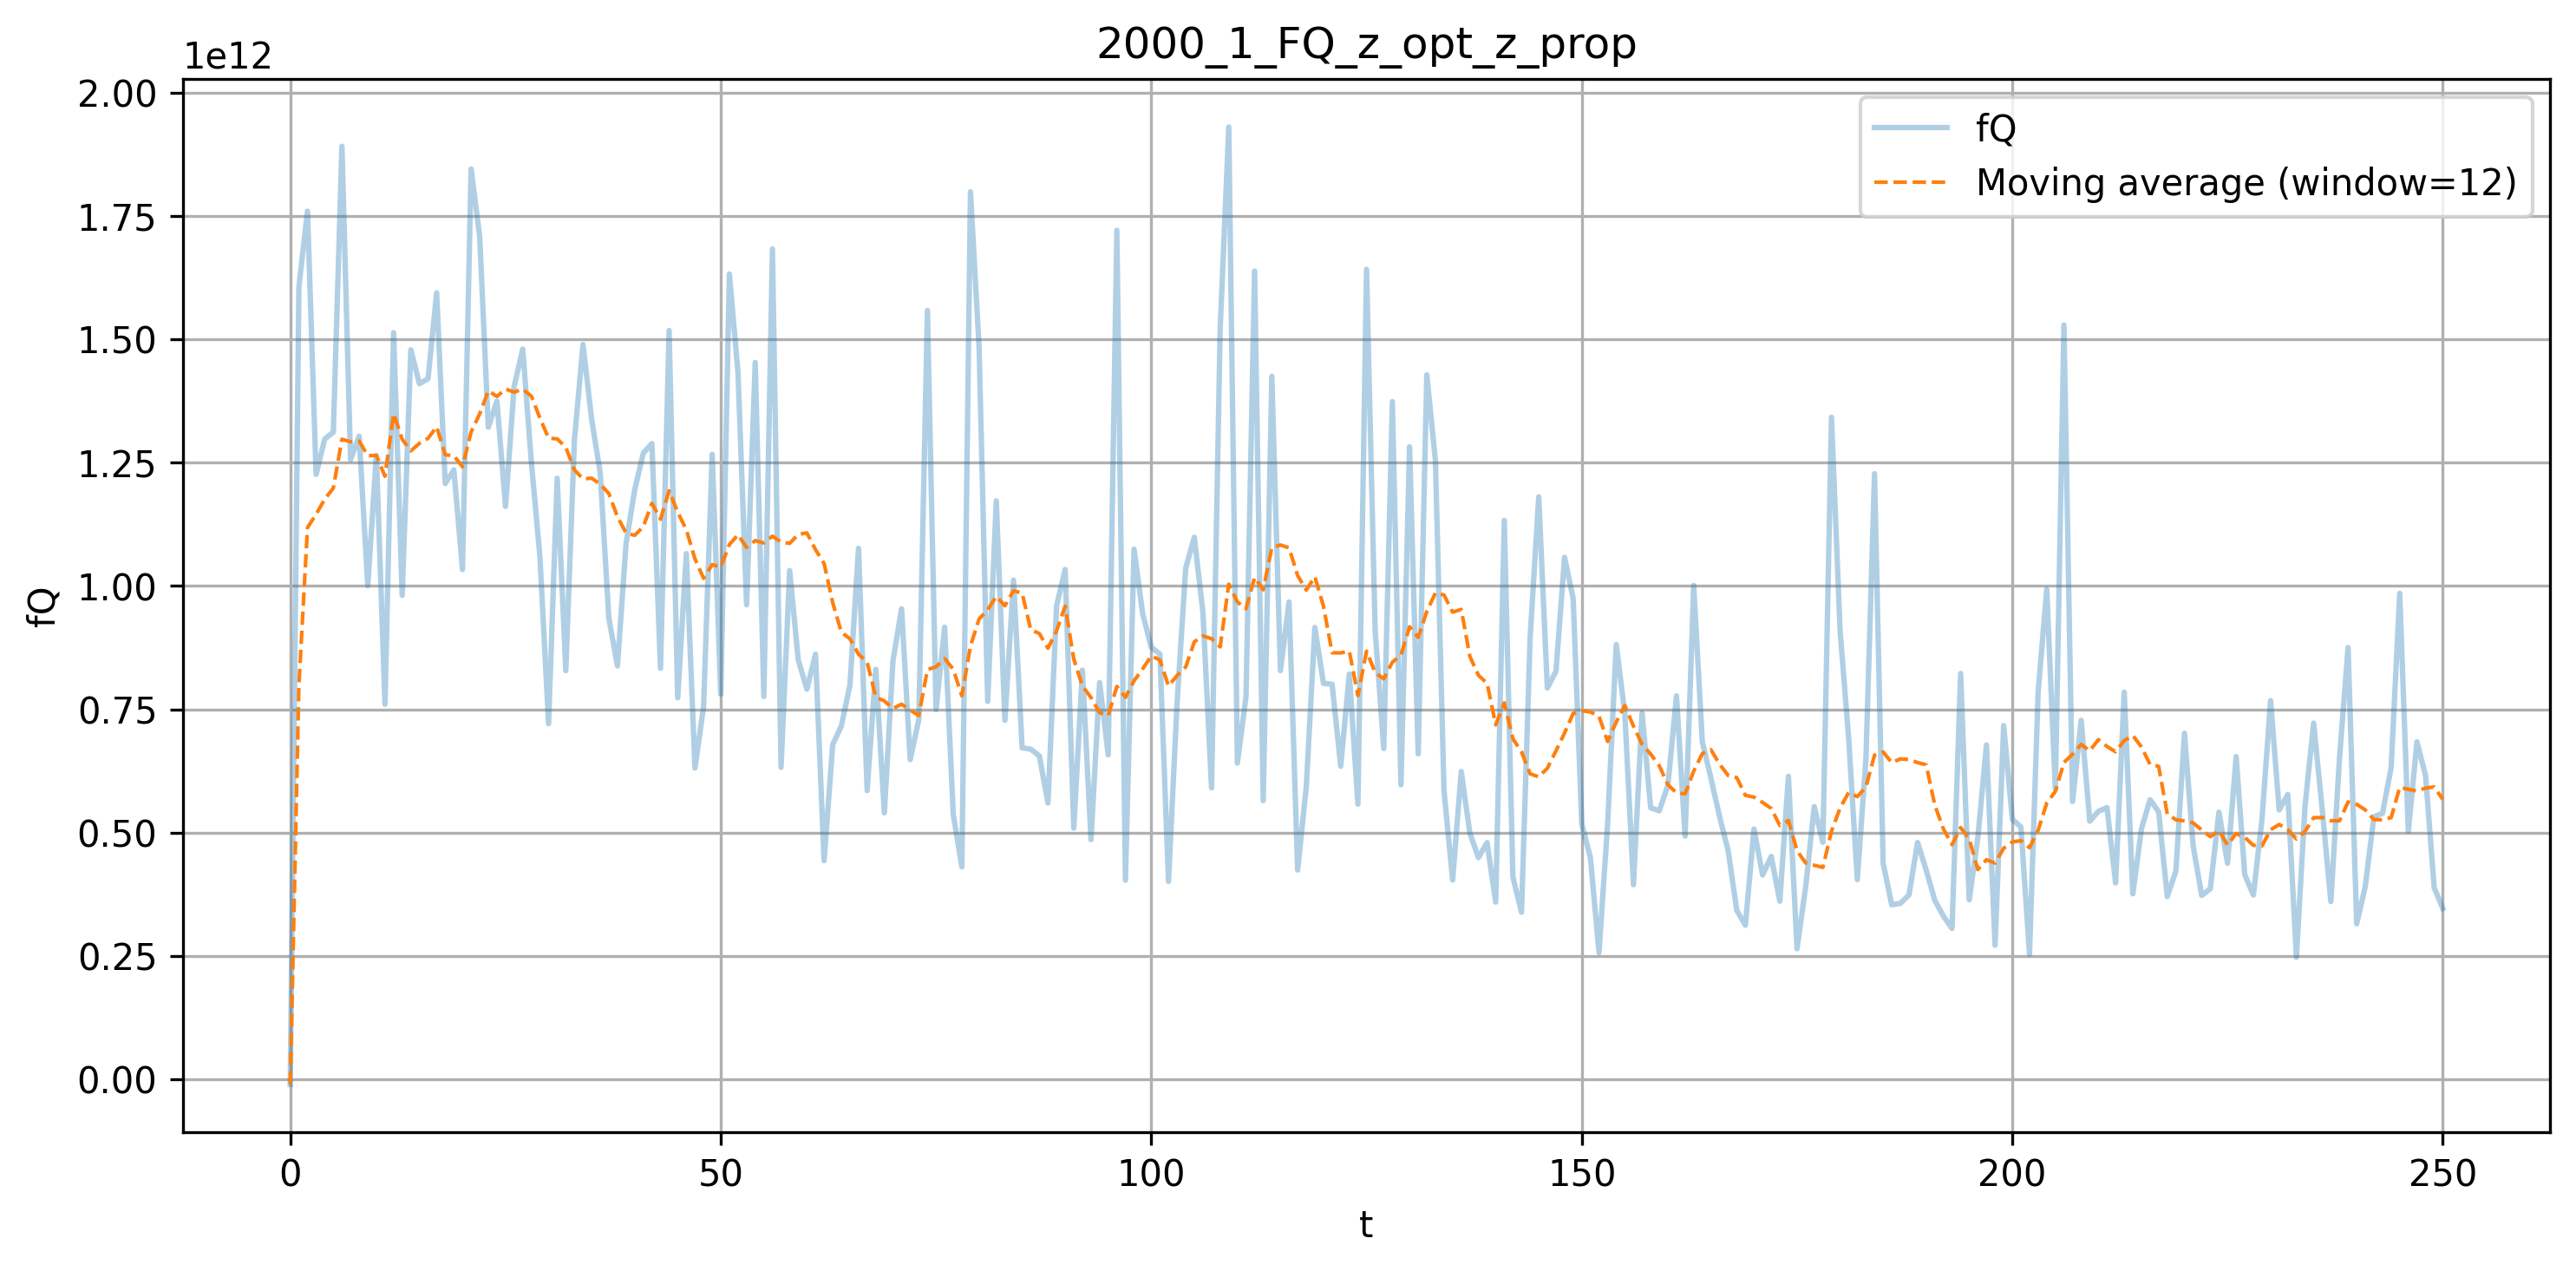
\includegraphics[width=\linewidth]{../Quantum-Annealing-for-solving-QUBO-Problems/test/Lambda_dinamico/ksp_2/lambda_div_3/2000_1_FQ_z_opt_z_prop.png}
    \caption{\(f_Q(z_t)\) con \(\lambda_2\)}
    \label{fig:fQ-zt-lambda2}
\end{subfigure}
\label{fig:confronto-hamming-ksp22}
\end{figure}

\begin{figure}[H]
\centering
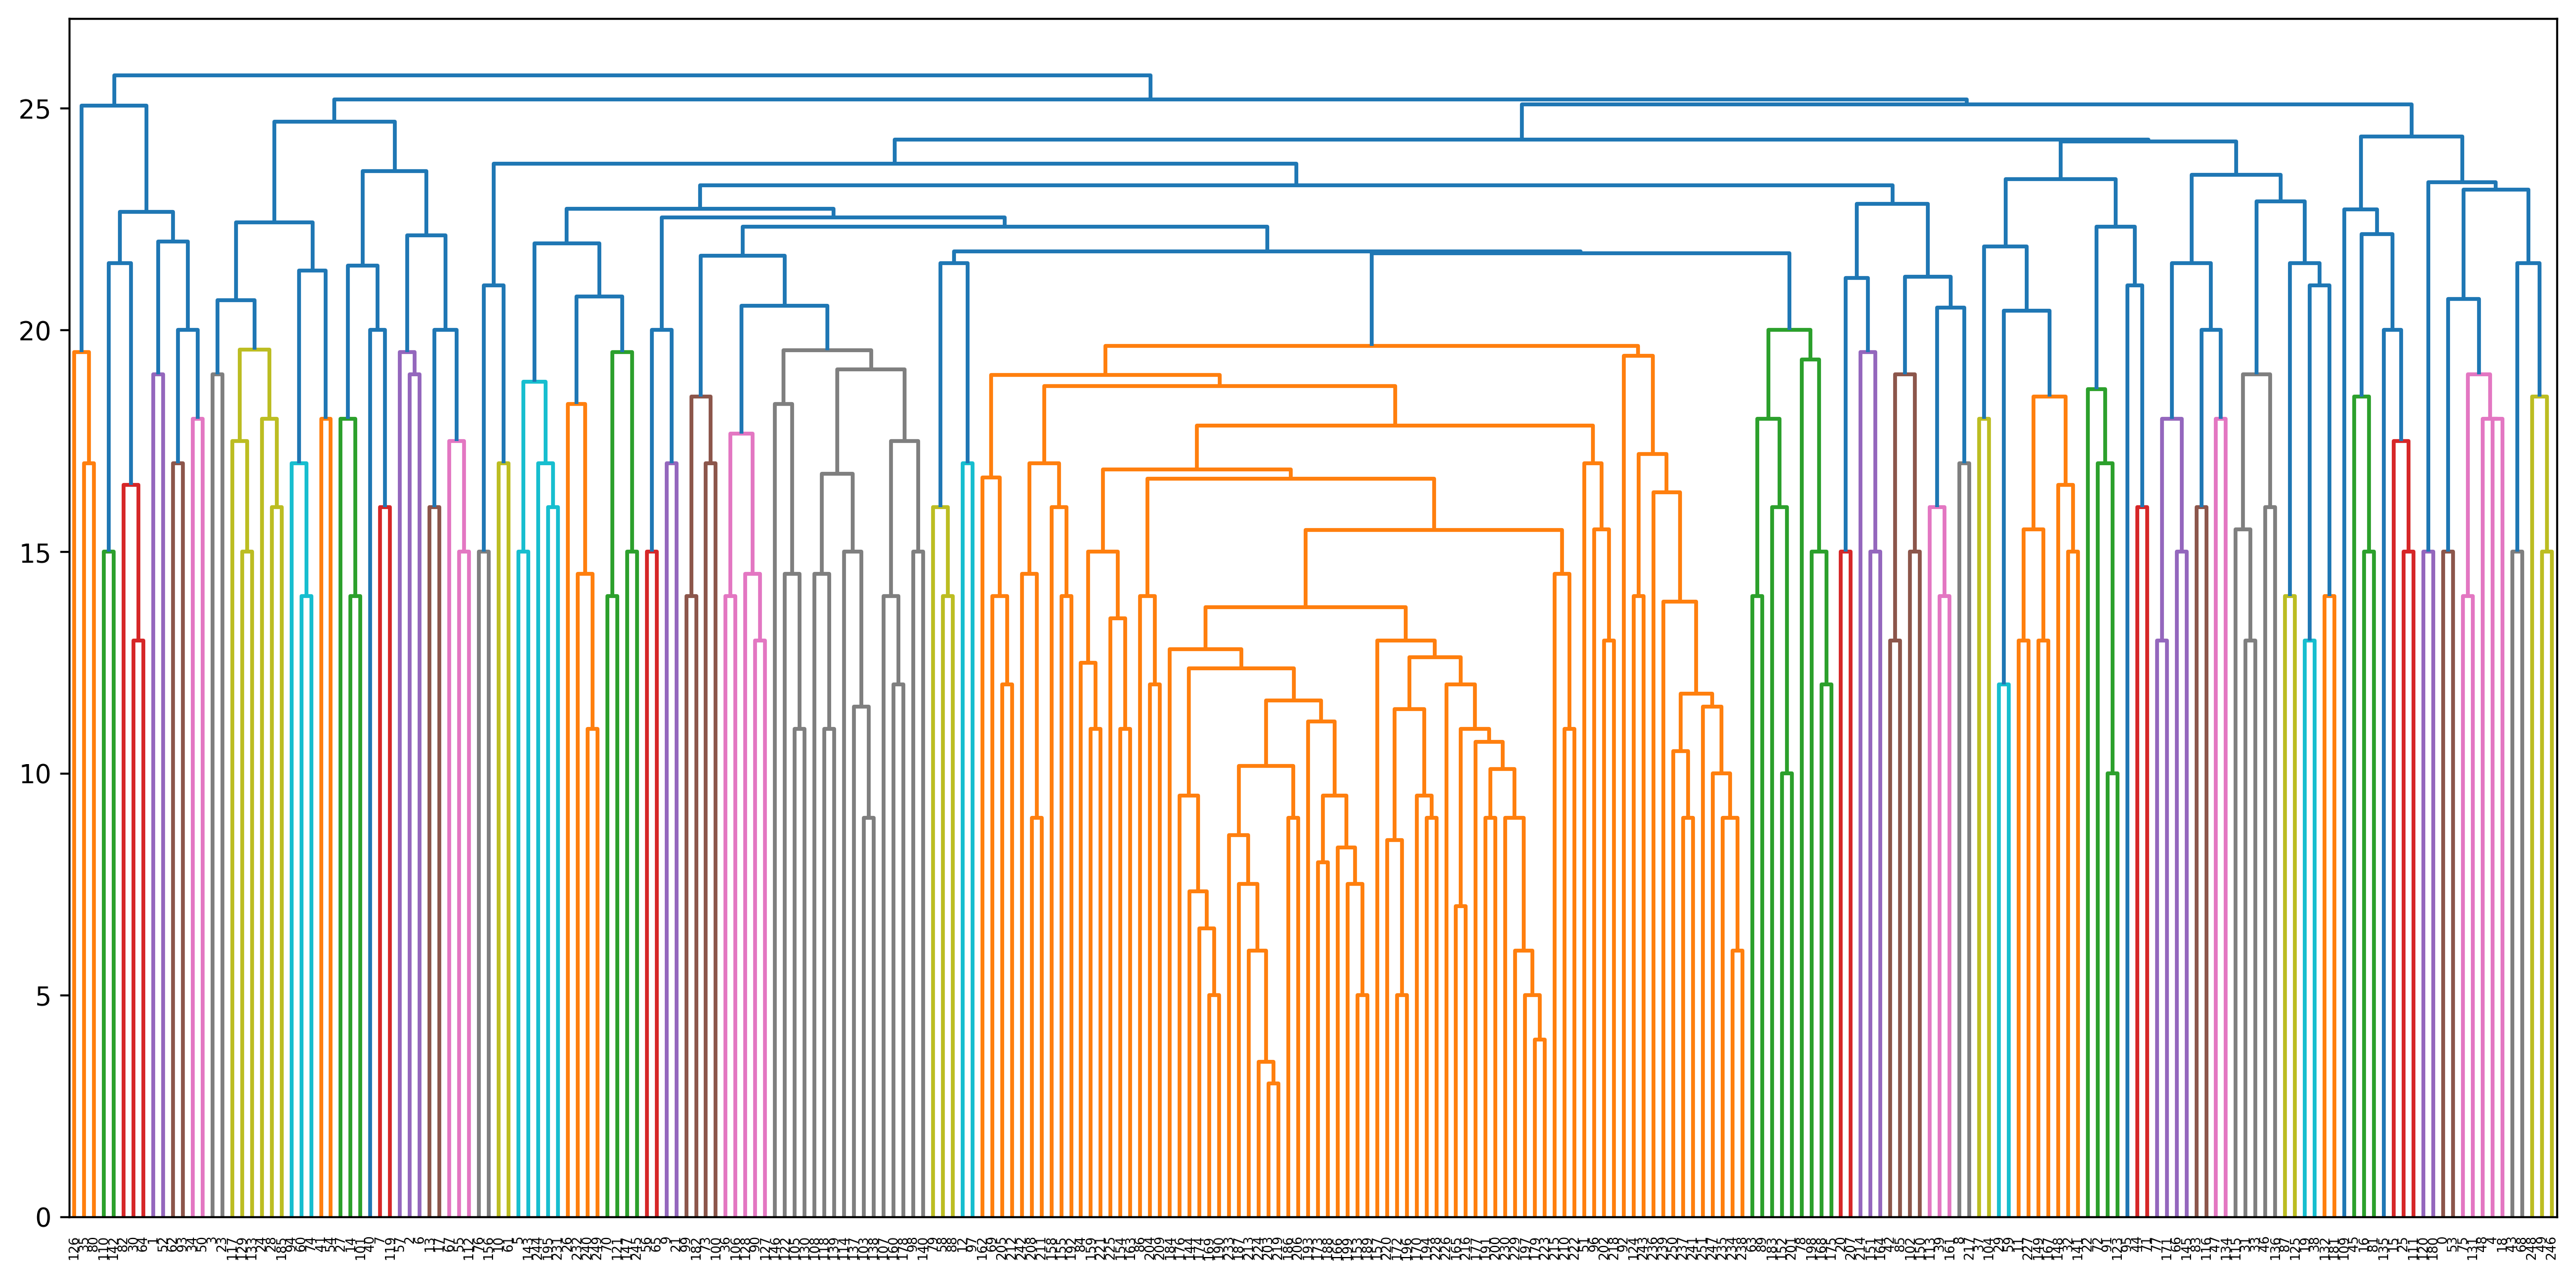
\includegraphics[width=\linewidth]{../Quantum-Annealing-for-solving-QUBO-Problems/test/Lambda_dinamico/ksp_2/lambda_div_3/dendrogram_2000_1.png}
\caption{Agglomerative Clustering Dendogram}
\label{fig:AgglomerativeClustering-ksp2}
\end{figure}

\subsection{Riassunto dati}

\begin{table}[h]
\centering
\begin{tabular}{lccc|ccc}
\hline
& \multicolumn{3}{c|}{\(\boldsymbol{\lambda_1}\)}
& \multicolumn{3}{c}{\(\boldsymbol{\lambda_2}\)} \\
\cline{2-7}

\textbf{Istanza}
& \(\boldsymbol{f_Q}\)
& \(\boldsymbol{N_{\mathrm{cluster}}}\)
& \(\boldsymbol{|C_{\max}|}\)
& \(\boldsymbol{f_Q}\)
& \(\boldsymbol{N_{\mathrm{cluster}}}\)
& \(\boldsymbol{|C_{\max}|}\) \\
\hline

\texttt{ksp\_1}
& -306.32
& 11
& 213
& -1455540.67
& 10
& 114 \\

\texttt{ksp\_3}
& 943.84
& 37
& 61
& 777361961.67
& 32
& 107 \\

\texttt{ksp\_2}
& 546064.29
& 45
& 108
& 218237506978.67
& 50
& 86 \\

\hline
\end{tabular}
\caption{Lambda modificato}
\label{tab:lambda_modificato}
\end{table}

\begin{table}[h]
\centering
\begin{tabular}{lccc|ccc}
\hline
& \multicolumn{3}{c|}{\(\boldsymbol{\lambda_1}\)}
& \multicolumn{3}{c}{\(\boldsymbol{\lambda_2}\)} \\
\cline{2-7}

\textbf{Istanza}
& \(\boldsymbol{f_Q}\)
& \(\boldsymbol{N_{\mathrm{cluster}}}\)
& \(\boldsymbol{|C_{\max}|}\)
& \(\boldsymbol{f_Q}\)
& \(\boldsymbol{N_{\mathrm{cluster}}}\)
& \(\boldsymbol{|C_{\max}|}\) \\
\hline

\texttt{ksp\_1}
& -279.97
& 6
& 225
& -1455540.67
& 12
& 126 \\

\texttt{ksp\_3}
& 18568.9
& 32
& 85
& 6552437129.67
& 30
& 87 \\

\texttt{ksp\_2}
& 663754.58
& 46
& 93
& 318472609310.67
& 50
& 95 \\

\hline
\end{tabular}
\caption{Originale con Decay factor}
\label{tab:originale}
\end{table}

\section{Interpretazione dei risultati}
Si noti come i grafici siano molti simili, l' unica sostanziale differenza che si può notare è che
nei test cases con la logica dell'aggiornamento di lambda cambiata i dati è come se fossero in media
più ''bassi'' il che spiega anche il motivo del perché si riesca a trovare un valore minore di \(f_Q\)
nonostante la ricerca sia simile.

\end{document}